\section{Experimental Results}
\subsection{Synthetic datasets}
%\begin{figure*}[htb]
%    \centering
%    \subfloat[ TwoCube]{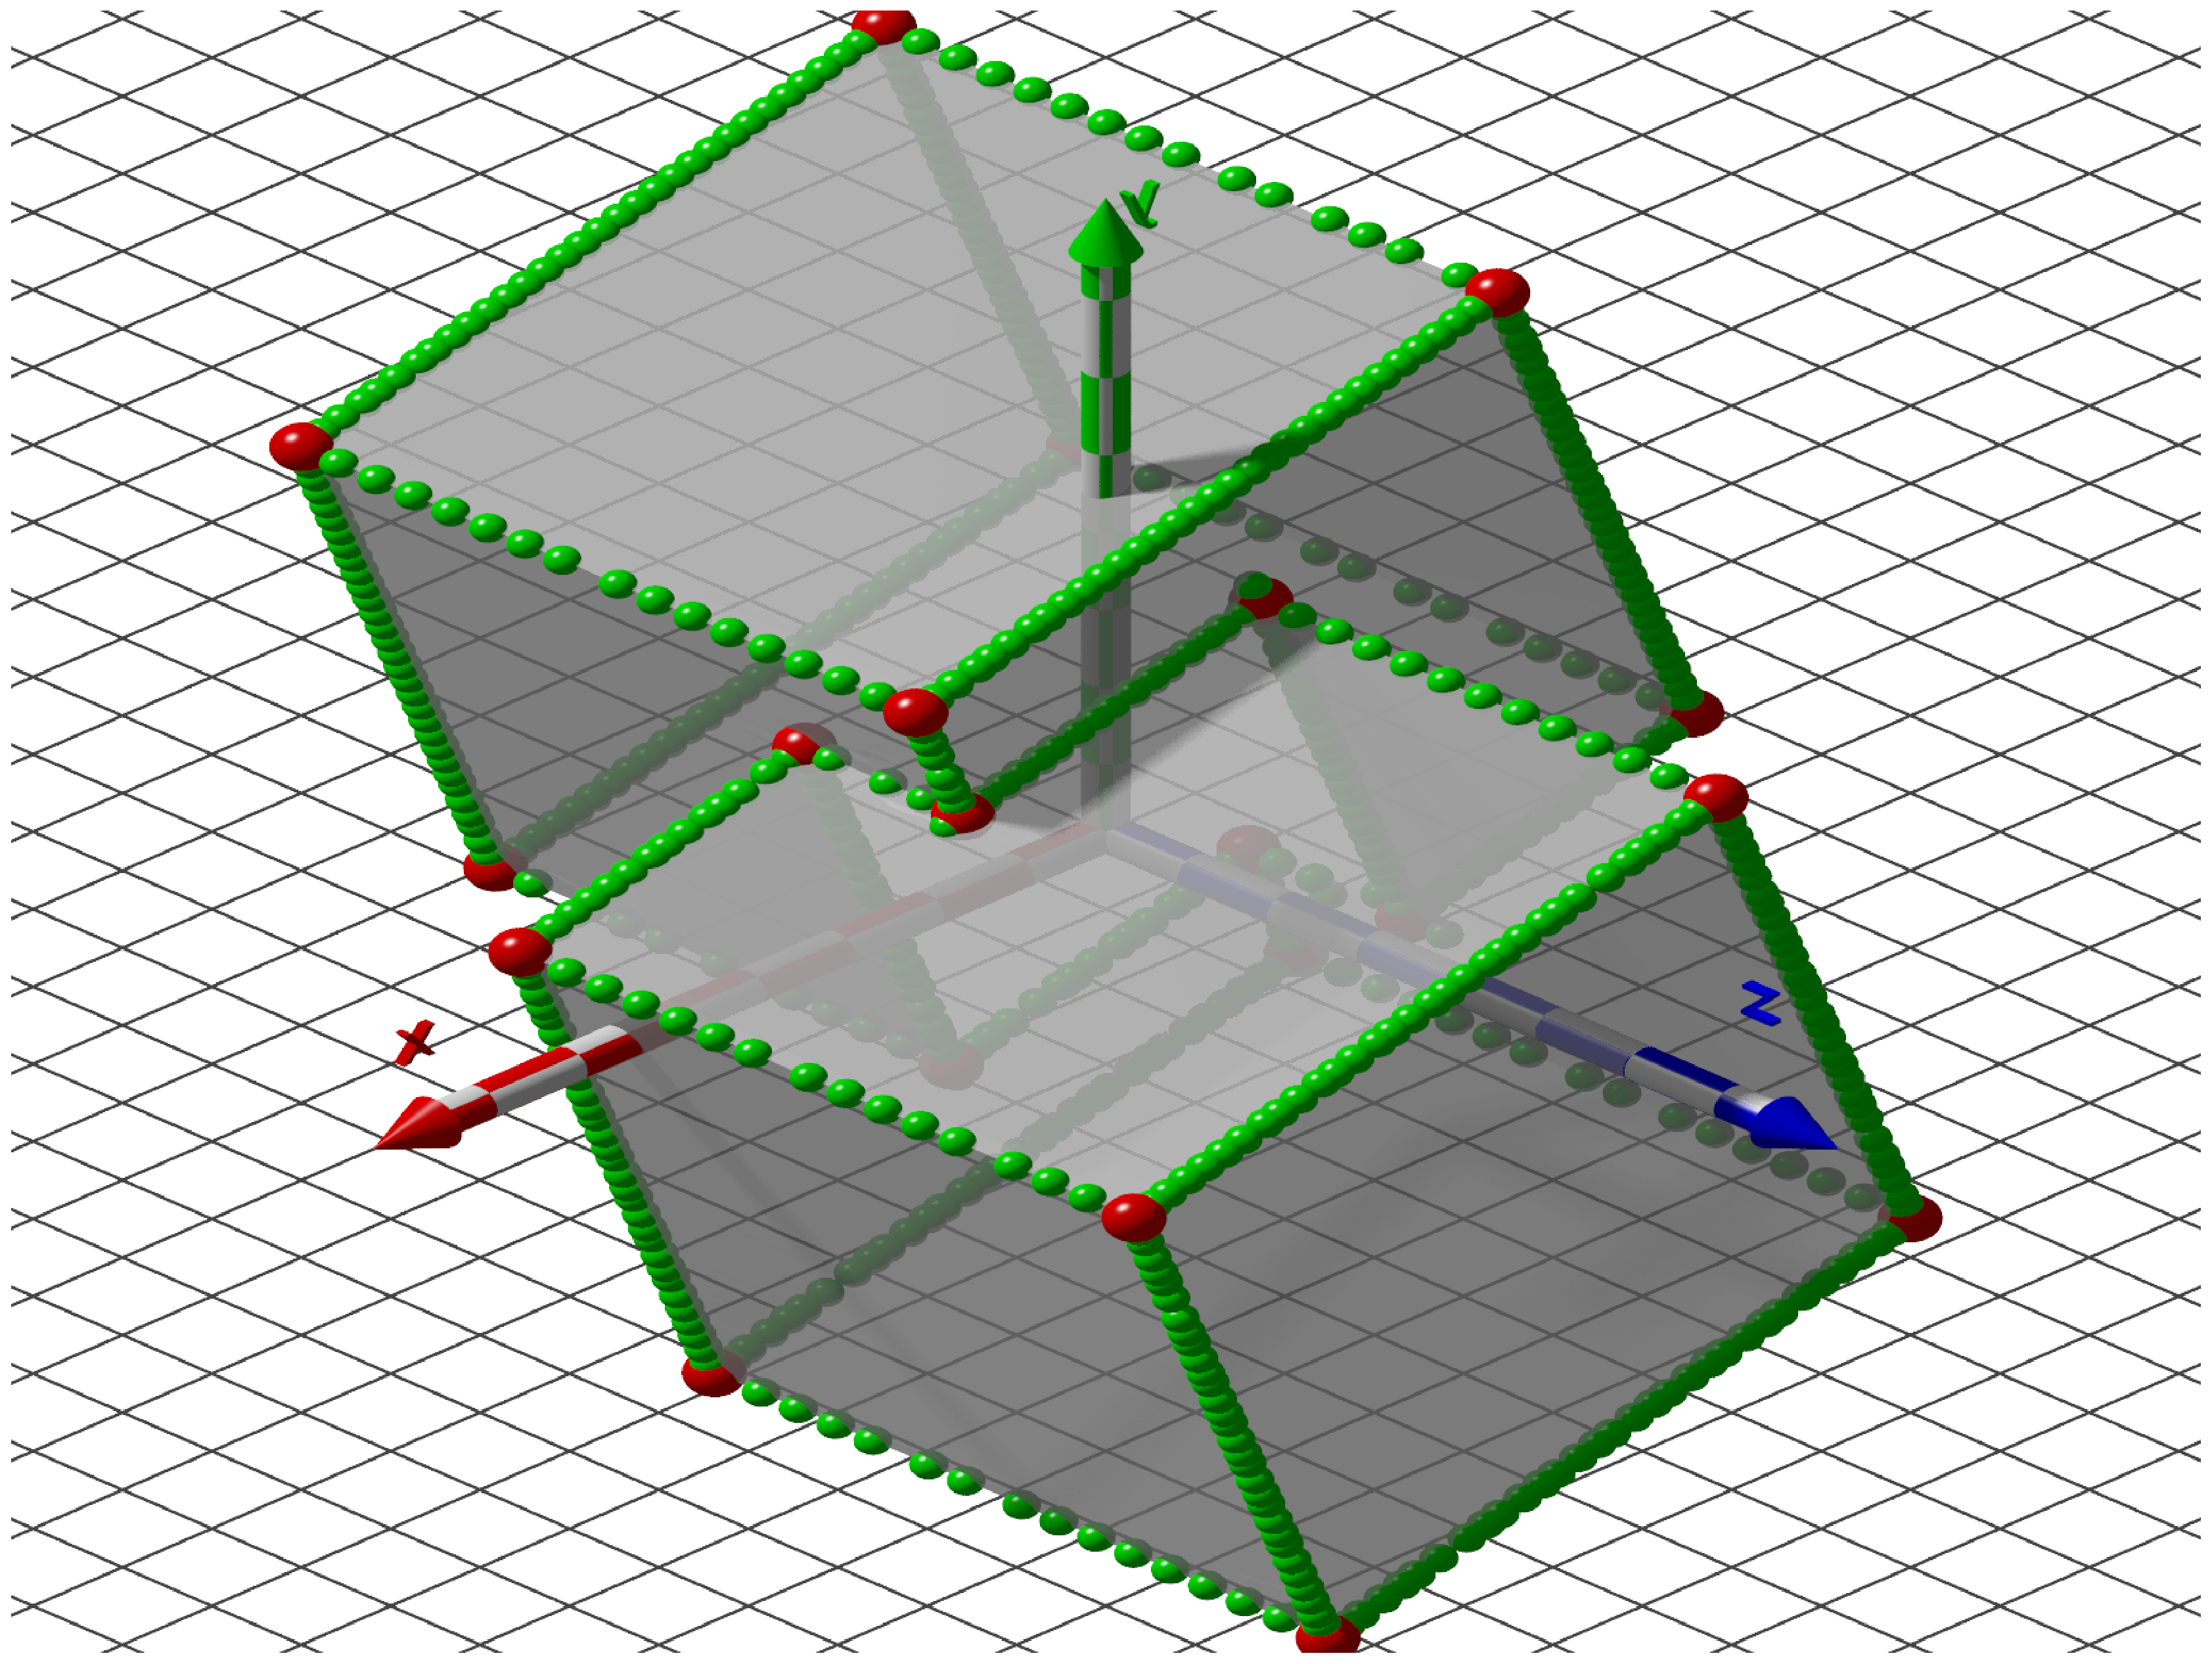
\includegraphics[width=0.2\linewidth]{images/twoCube.B.eps}\label{fig:TwoCube}}
%    \subfloat[Flange]{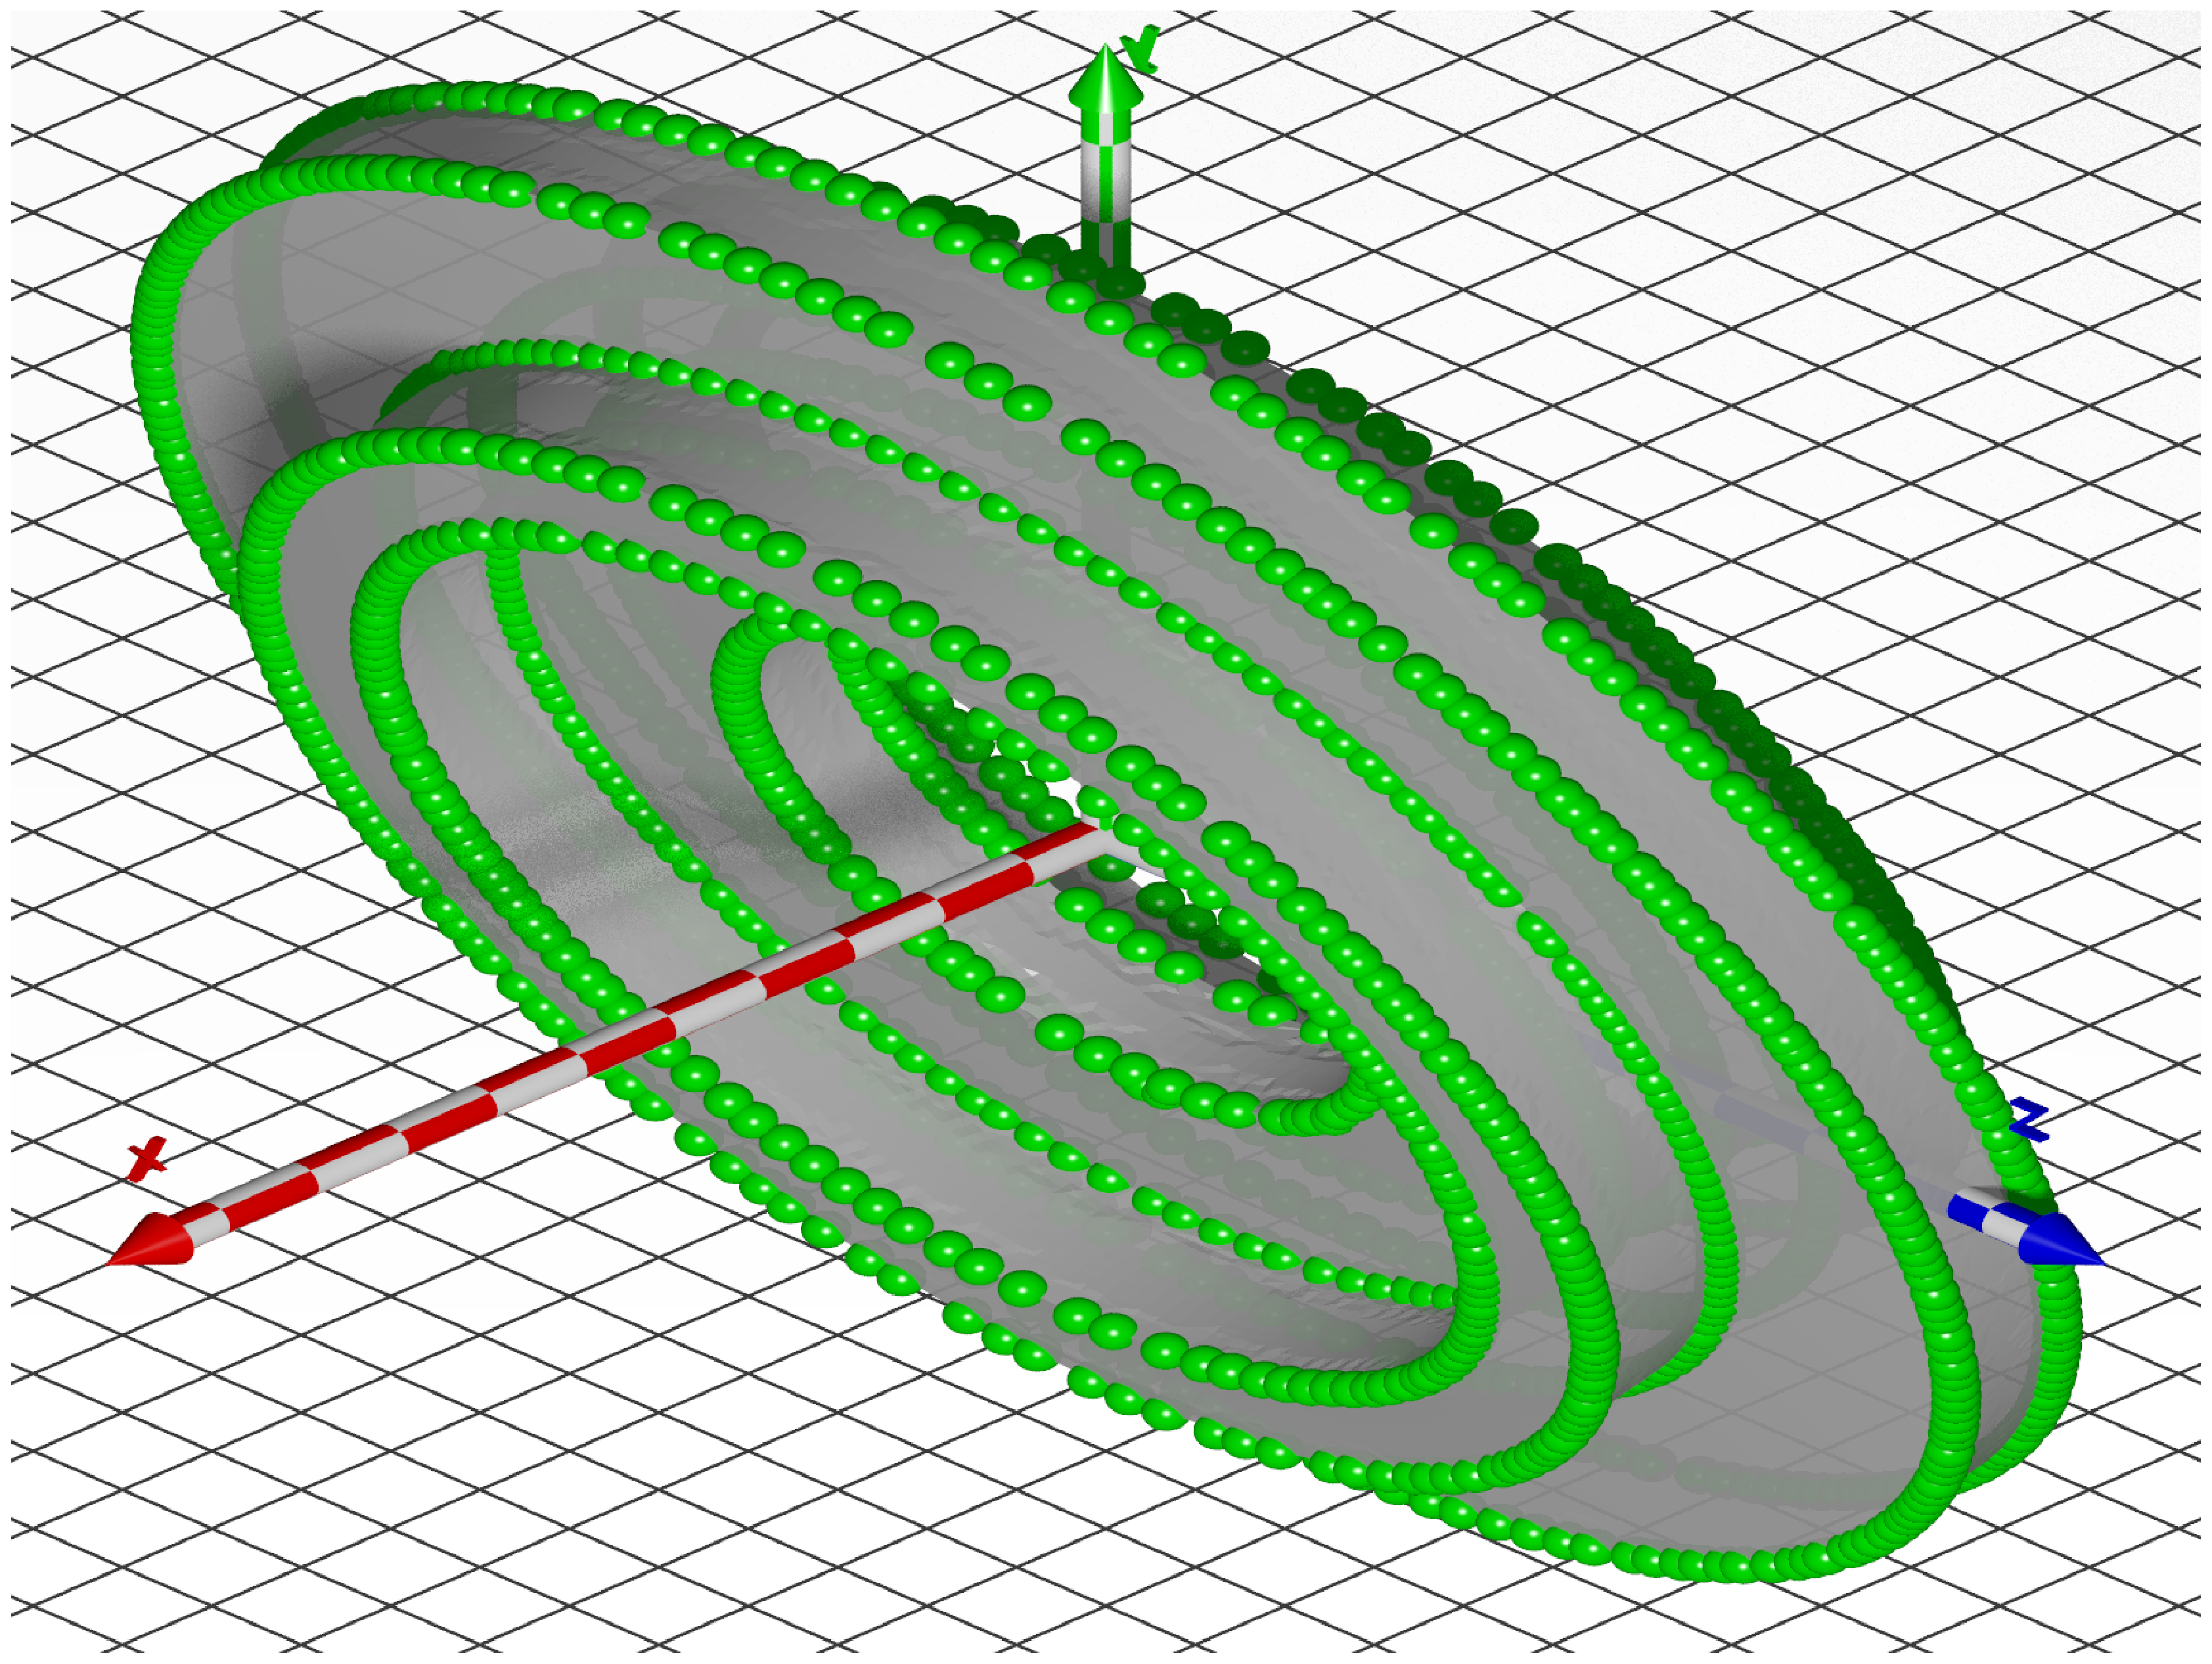
\includegraphics[width=0.2\linewidth]{images/flange.C2.new.eps}\label{fig:flange}}
%    \subfloat[Annulus]{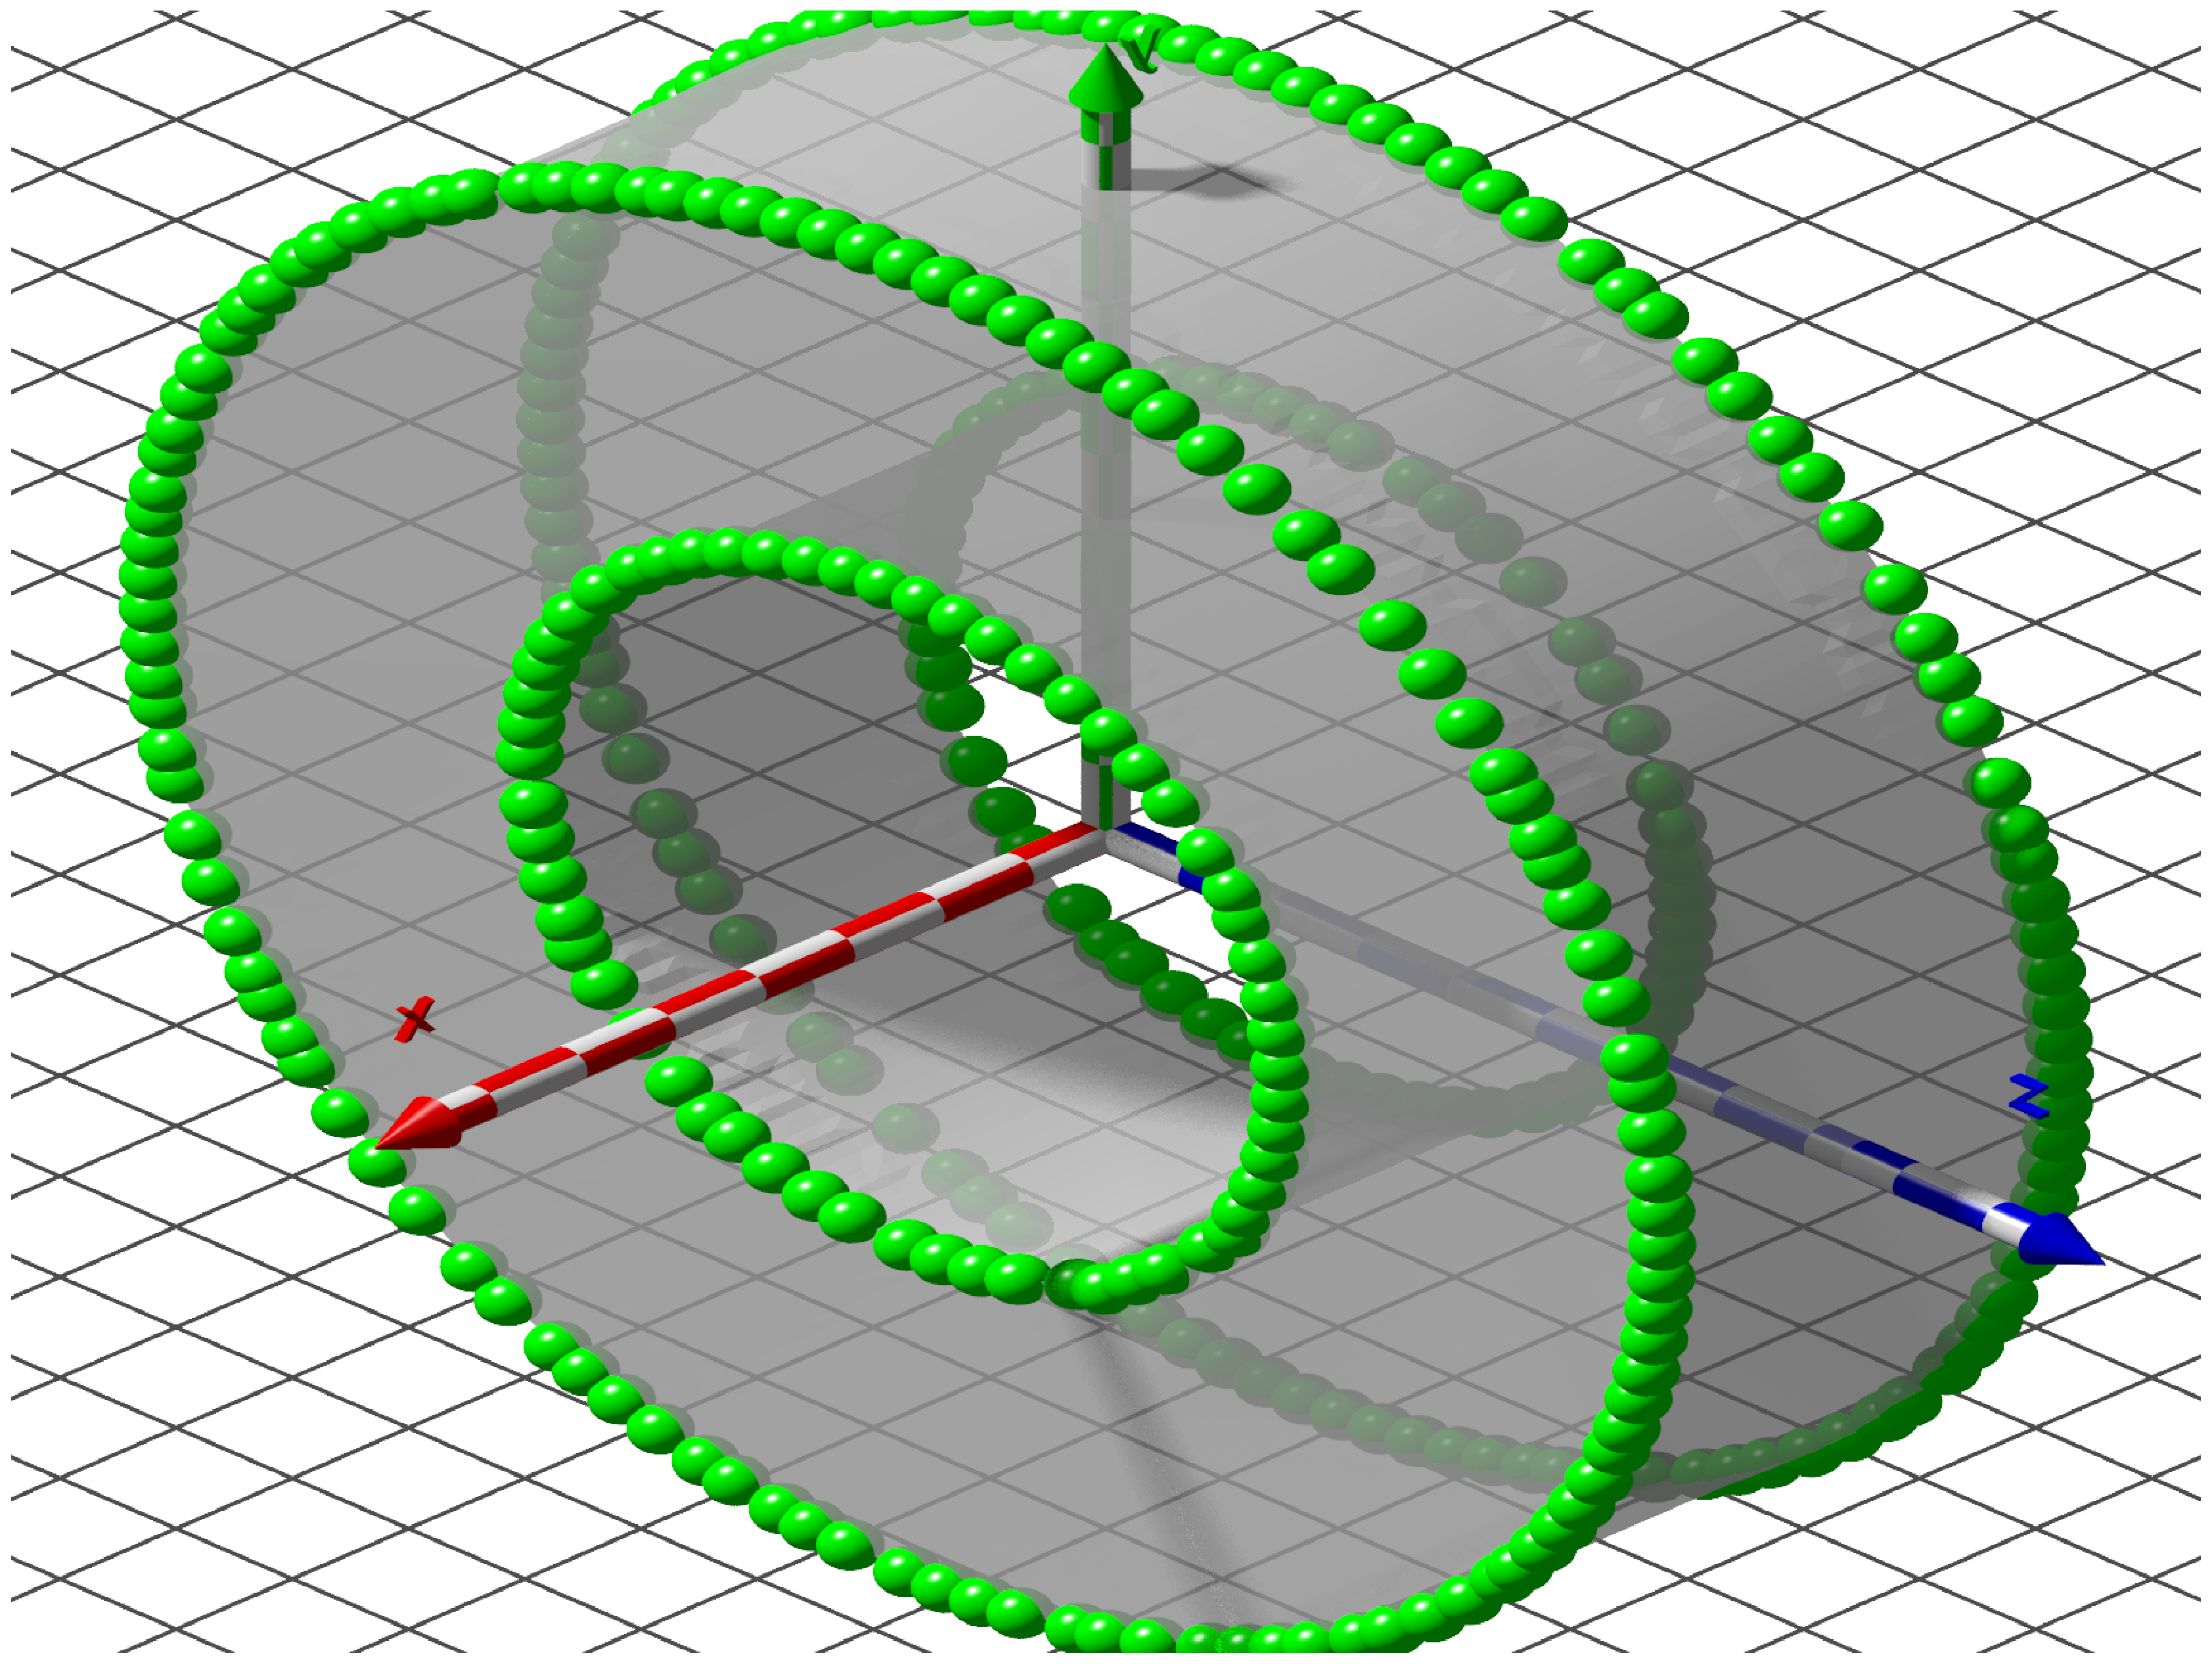
\includegraphics[width=0.2\linewidth]{images/annulus.eps}\label{fig:annulus}}
%    \subfloat[Cone]{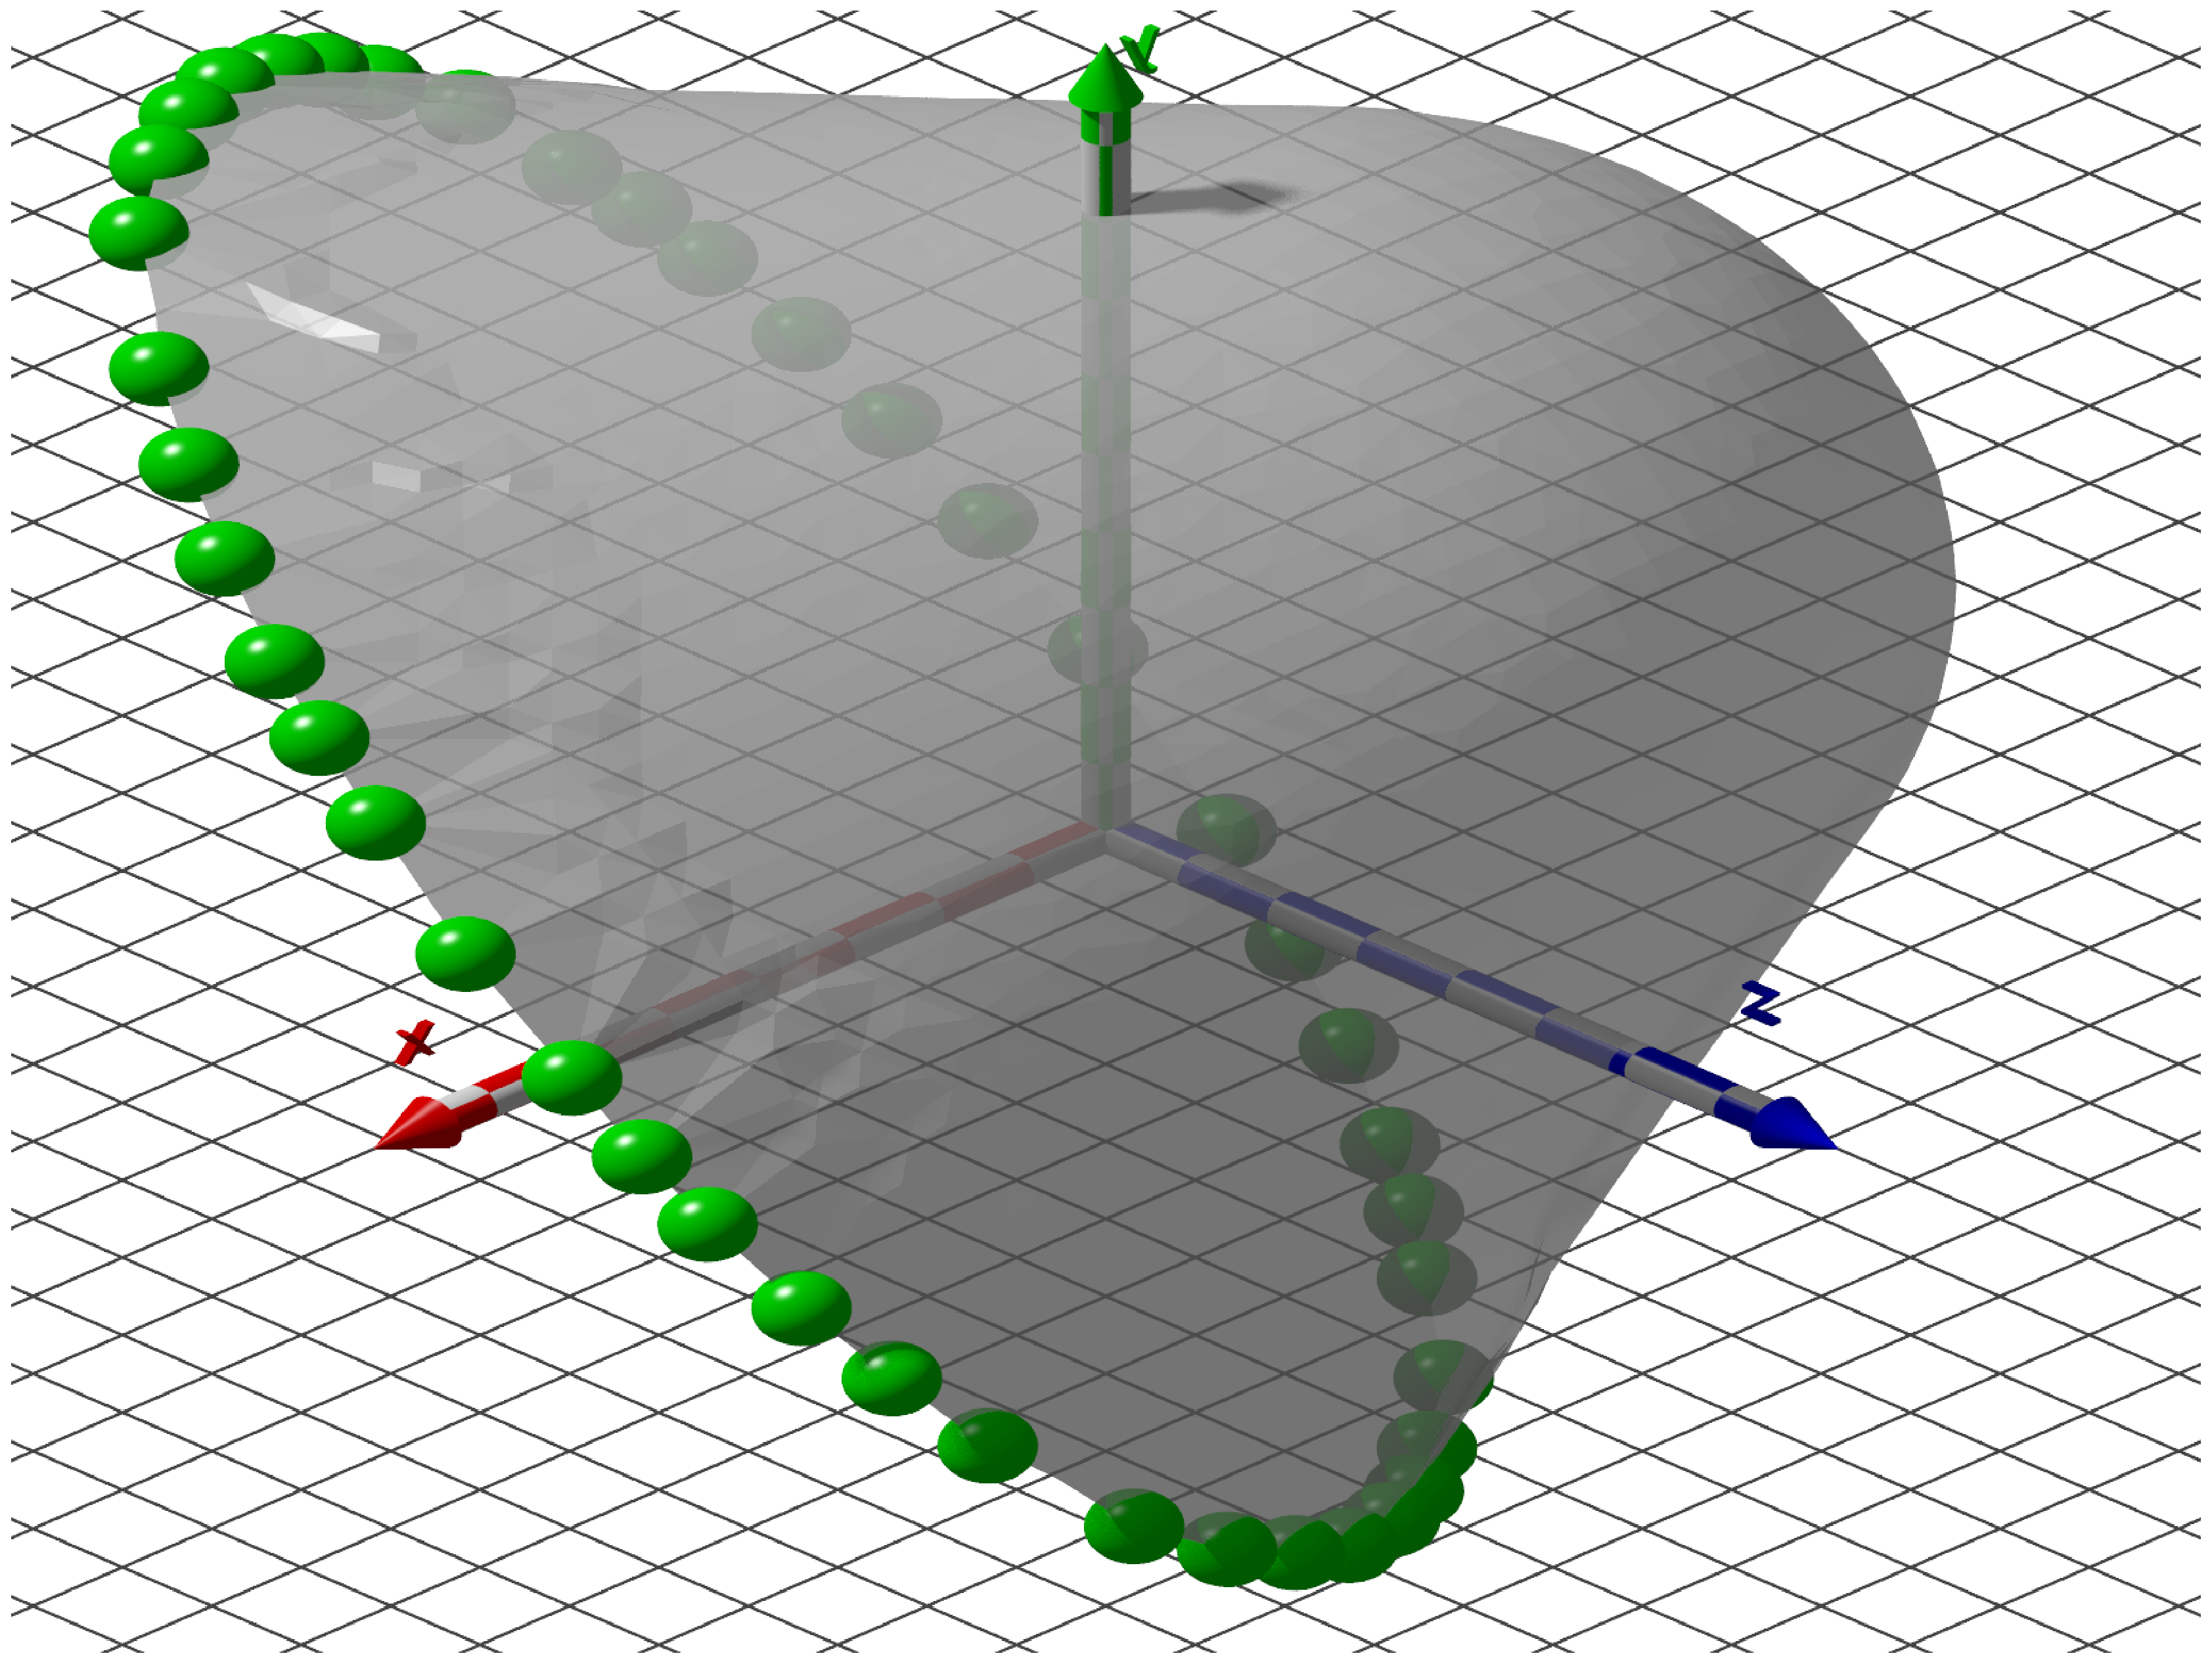
\includegraphics[width=0.2\linewidth]{images/cone.eps}\label{fig:cone}}
%    \subfloat[Cannon]{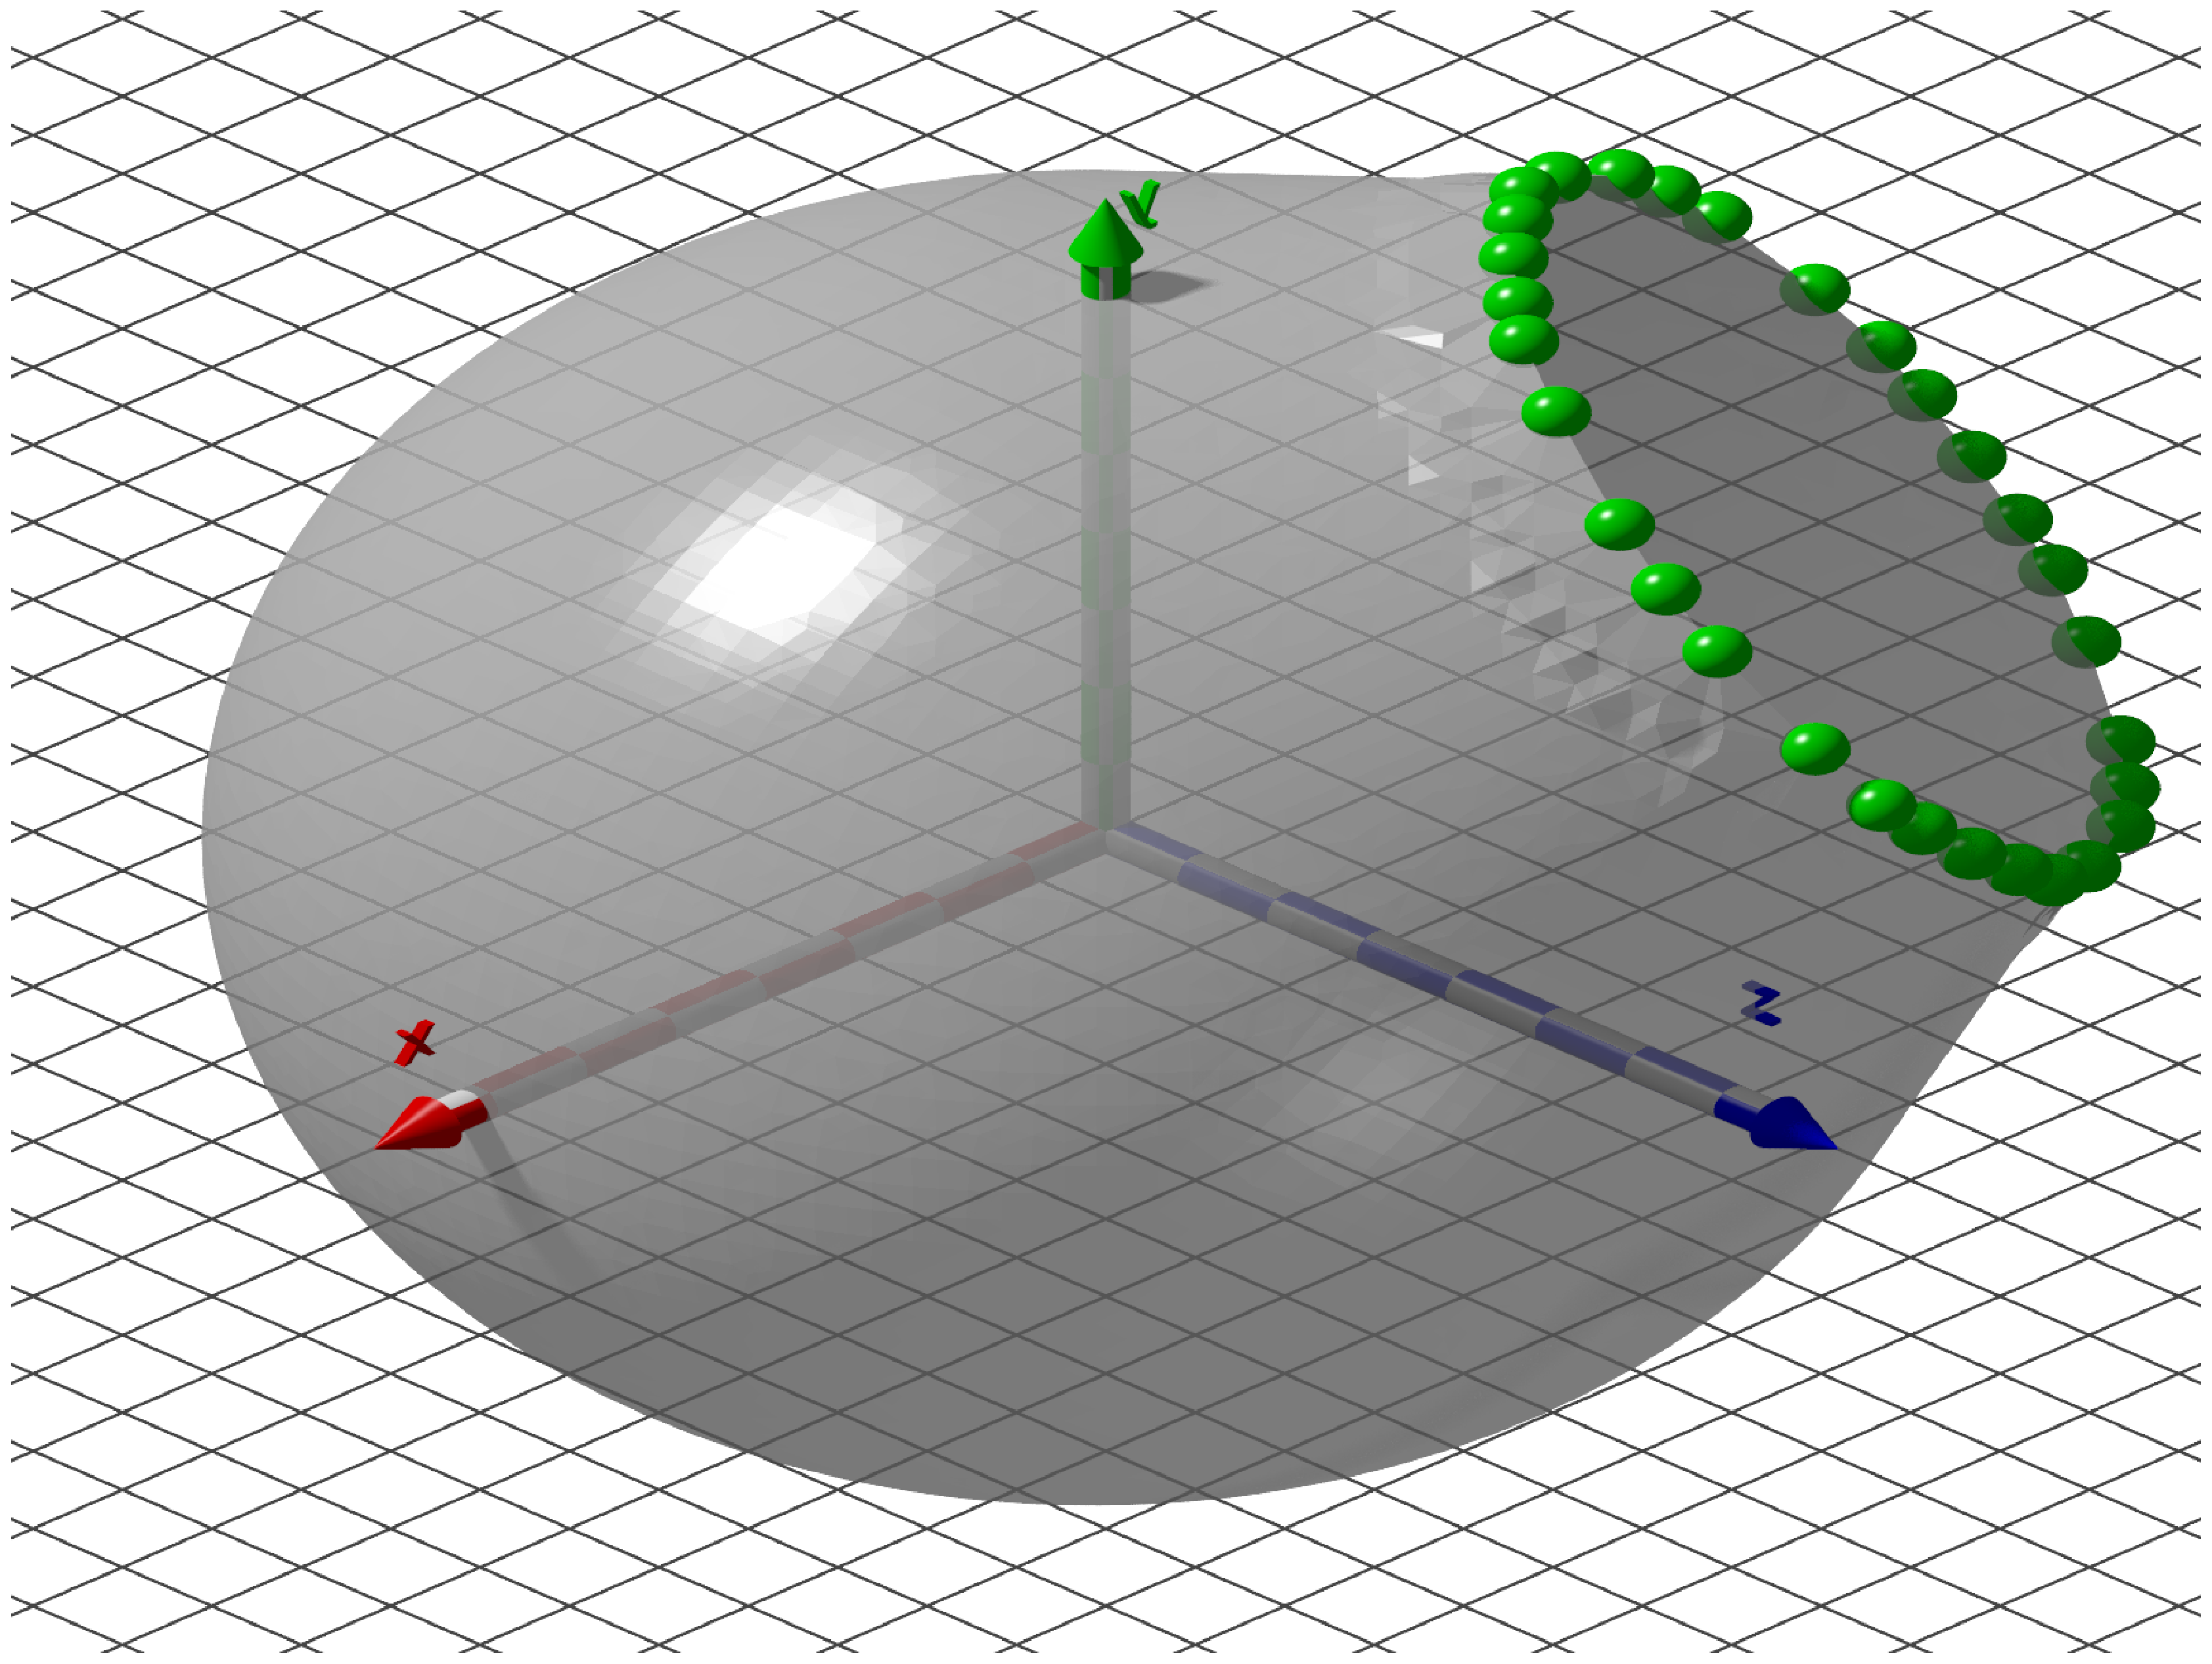
\includegraphics[width=0.2\linewidth]{images/cannon.eps}\label{fig:cannon}}
%    \caption{Synthetic datasets. Table~\ref{table:SynDataInfo} provides more information, Isosurface vertices associated with three large eigen values (Section~\ref{sec:computeSharpPoints}) are corners and marked in red. Selected edge isovertices are marked in green.}
%    \label{fig:SynData}
%\end{figure*}
\begin{table}[htb]
	\centering
	\begin{tabular}{|c c c c|} 
		\hline
		Name & ASize & Spacing & ARotation \\ [0.5ex] 
		\hline 
		\textit{Cube}  & 100 & 1 1 1 & 1 1 1\\
		\textit{Annulus} & 100 & 1 1 1 &  1 0 0\\ 
		\textit{TwoCube} & 150 & 0.2 0.2 0.4 &  1.732 0.577 0\\ 
		\textit{Flange} & 150 & 0.2 0.2 0.4 &  1.732 0.577 0\\ 
        \textit{Smooth-tip Cone} & 100 & 1 1 1 &  -1 1 1\\ 
        \textit{Cannon} & 100 & 1 1 1 &  -1 1 1\\ 
		\hline
	\end{tabular}
	\caption{Synthetic dataset information, the size of the datasets is $ASize^3$. The tilt of the axis of the dataset, is a line joining the origin to ARotation.}
	\label{table:SynDataInfo}
\end{table}
We tested our algorithm on a large number of synthetic datasets with varying spacings and axis rotations, here we show 6 representative elements; Table \ref{table:SynDataInfo} and figure~\ref{fig:SynData}.

\textbf{Description}:
The \emph{Cube} dataset samples a scalar field $f:\colon\Rthree \to \R$, where $f(p)$ is the minimum of the $L_{\infty}$ distance to a single point. Tilted cubes are made from orthogonal frames other than the standard \emph{x,y} and \emph{z} axis. The \emph{TwoCube} dataset, uses the minimum of the $L_{\infty}$ distance to two points. The \emph{TwoCube} dataset tests the performance of our algorithm on sharp corners and saddle points. 
The \emph{Annulus} dataset is minimum of the distance to a cylinder and the distance to a plane orthogonal to the cylinder.
By adding constants to these distances, we can create annulli with arbitrary heights and radii.
The \emph{Flange} datasets is the minimum of two \emph{Annulus} data sets,
one with flat, wide annulii and one with tall thin annulii.
Isosurfaces in these datasets are flanges with sharp concave and convex edges.
The \emph{Cone} data set is the minimum of the distance to a cone and to an orthogonal plane.
The distance to the cone near the tip is the distance to the point at the tip of the cone.
The isosurface around the tip is part of a sphere.
The \emph{Cone} dataset has acute dihedral angles of $60^\circ$.
The \emph{Cannon} dataset is the combination of the distance to a cone, the distance to an orthogonal plane
and the distance to a point.
The \emph{Cannon} dataset has obtuse dihedral angles of $120^\circ$.
\emph{Flange} and \emph{TwoCube} are challenging datasets, the spacings on these are not uniform and they are not axis aligned.
\emph{Cone} and \emph{Cannon} are also non-axis aligned (Table\ref{table:SynDataInfo}).

\begin{figure*}[htb]
    \centering
    \subfloat[Correct Gradients]{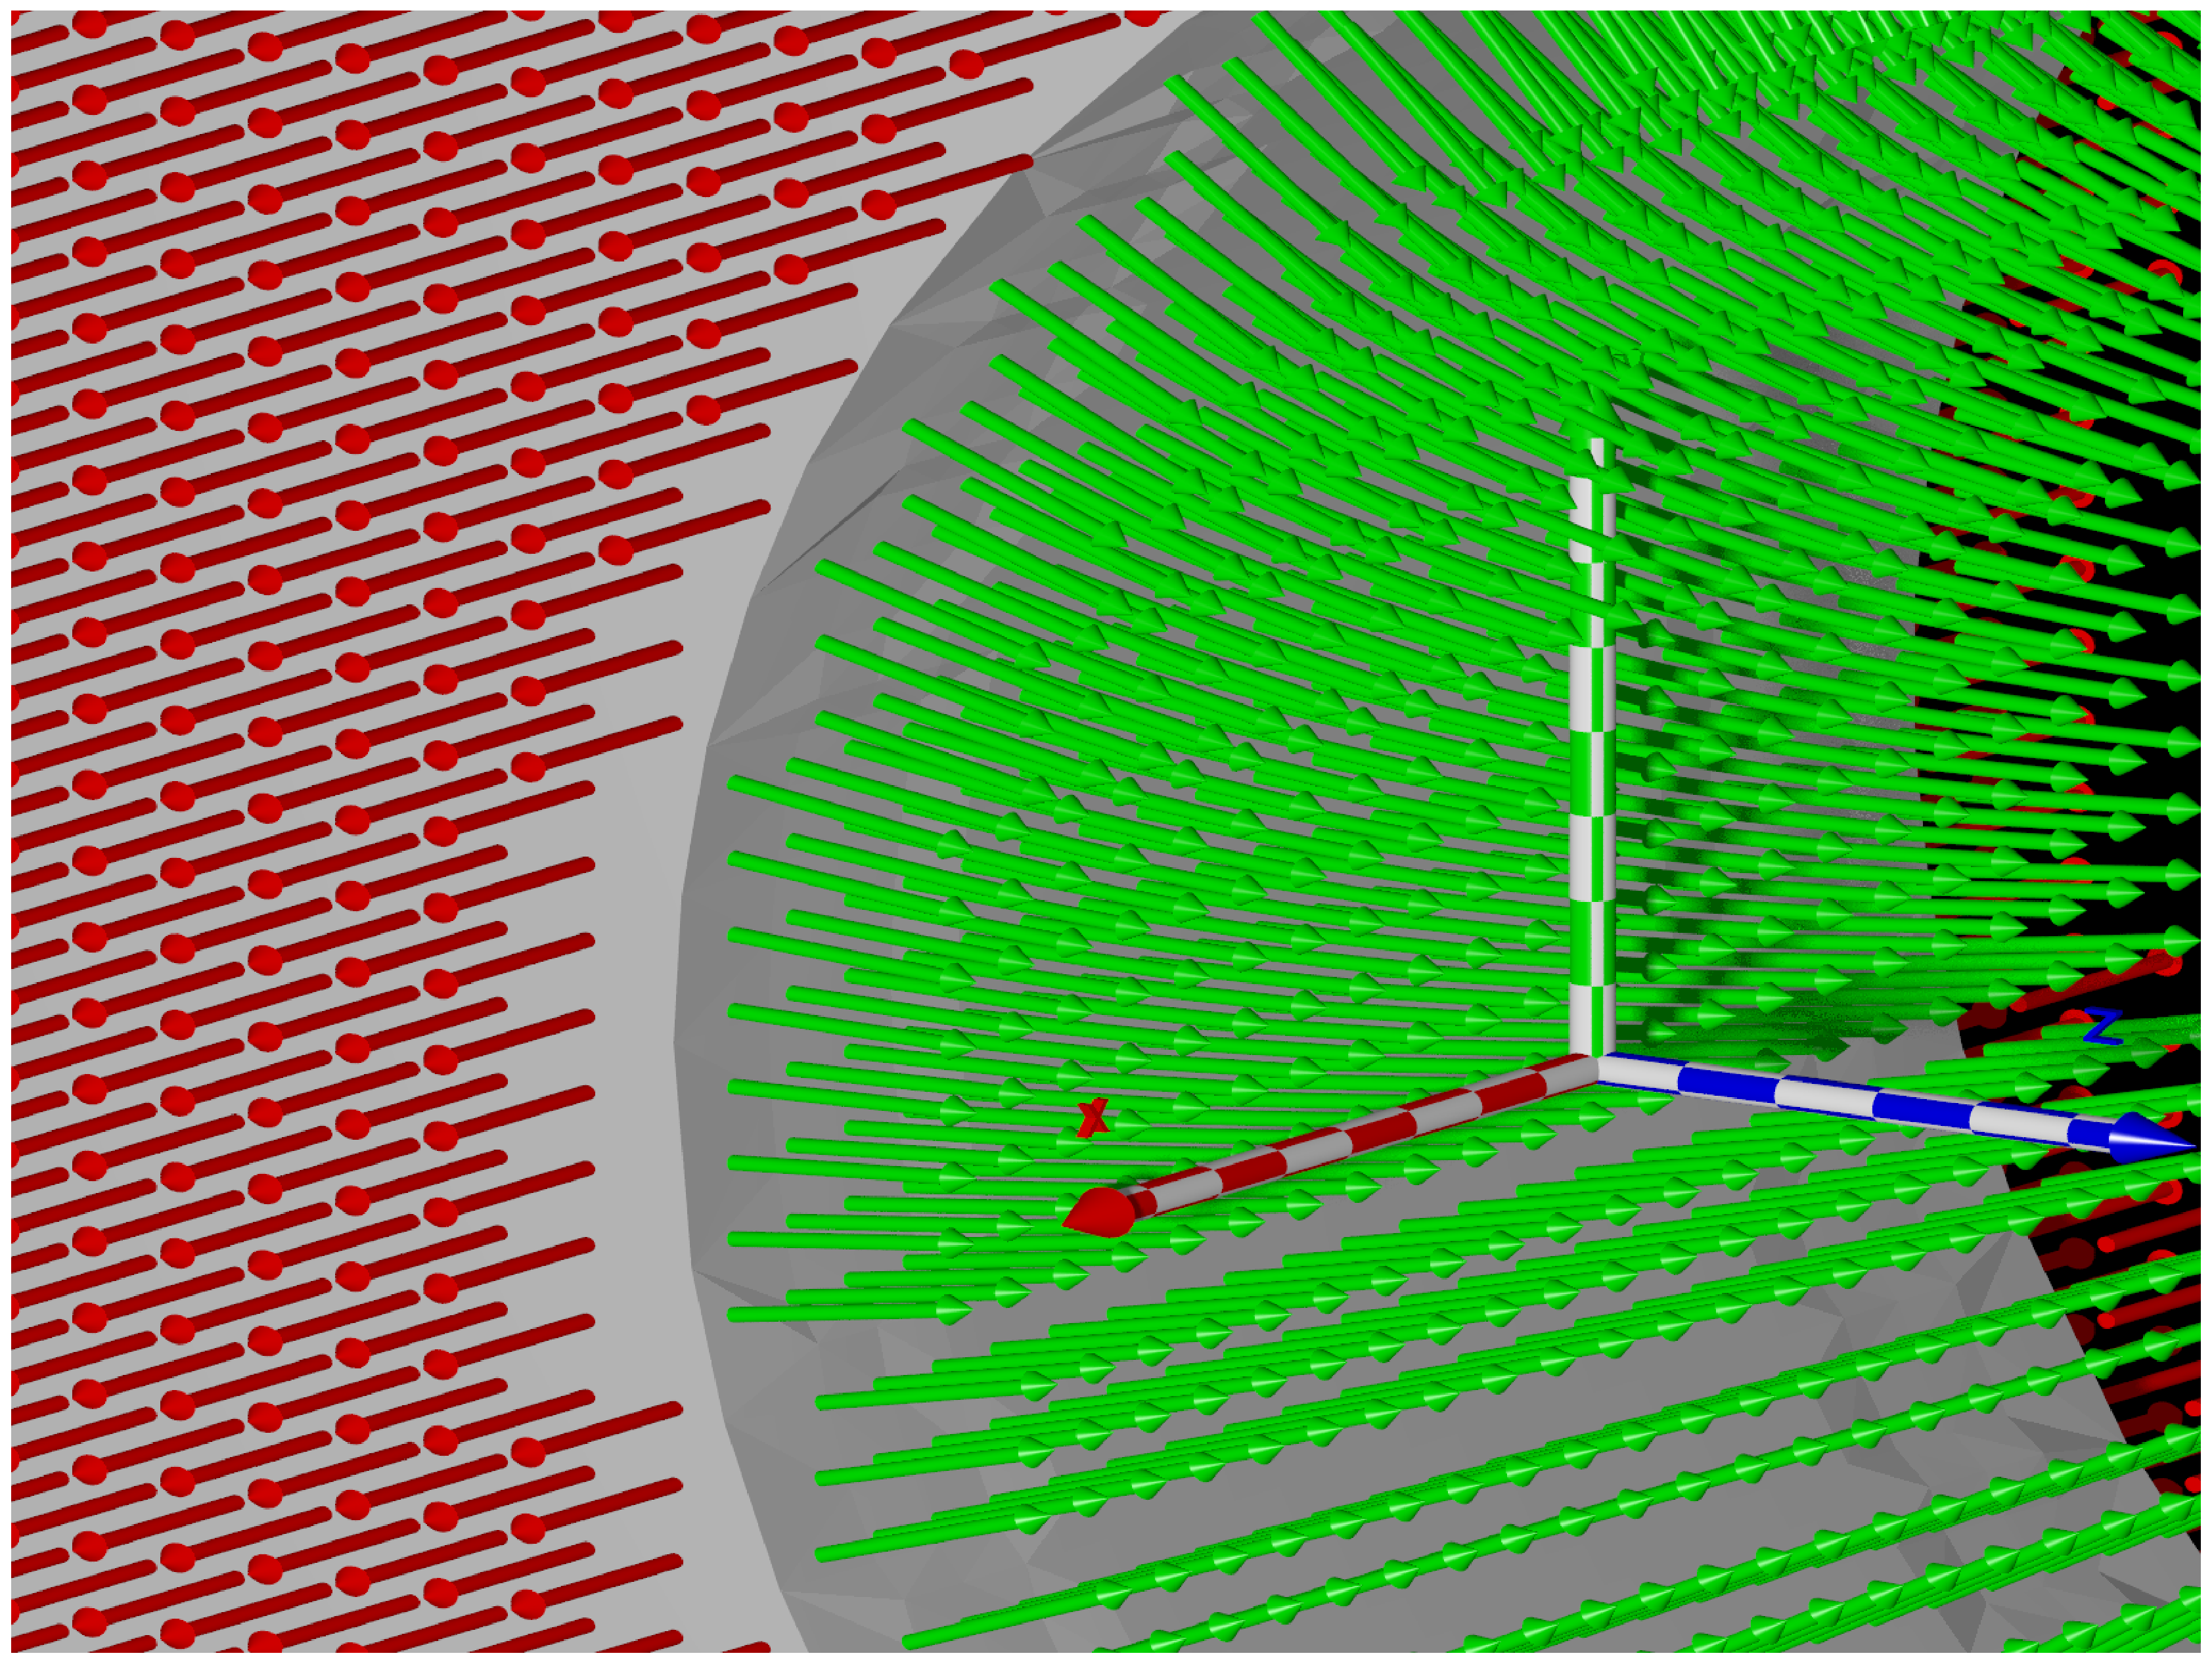
\includegraphics[width=0.3\linewidth]{images/annulus.gradcompare.correct.eps}\label{fig:annulus:correct}}\quad
    \subfloat[Edge dist. 1 predictions]{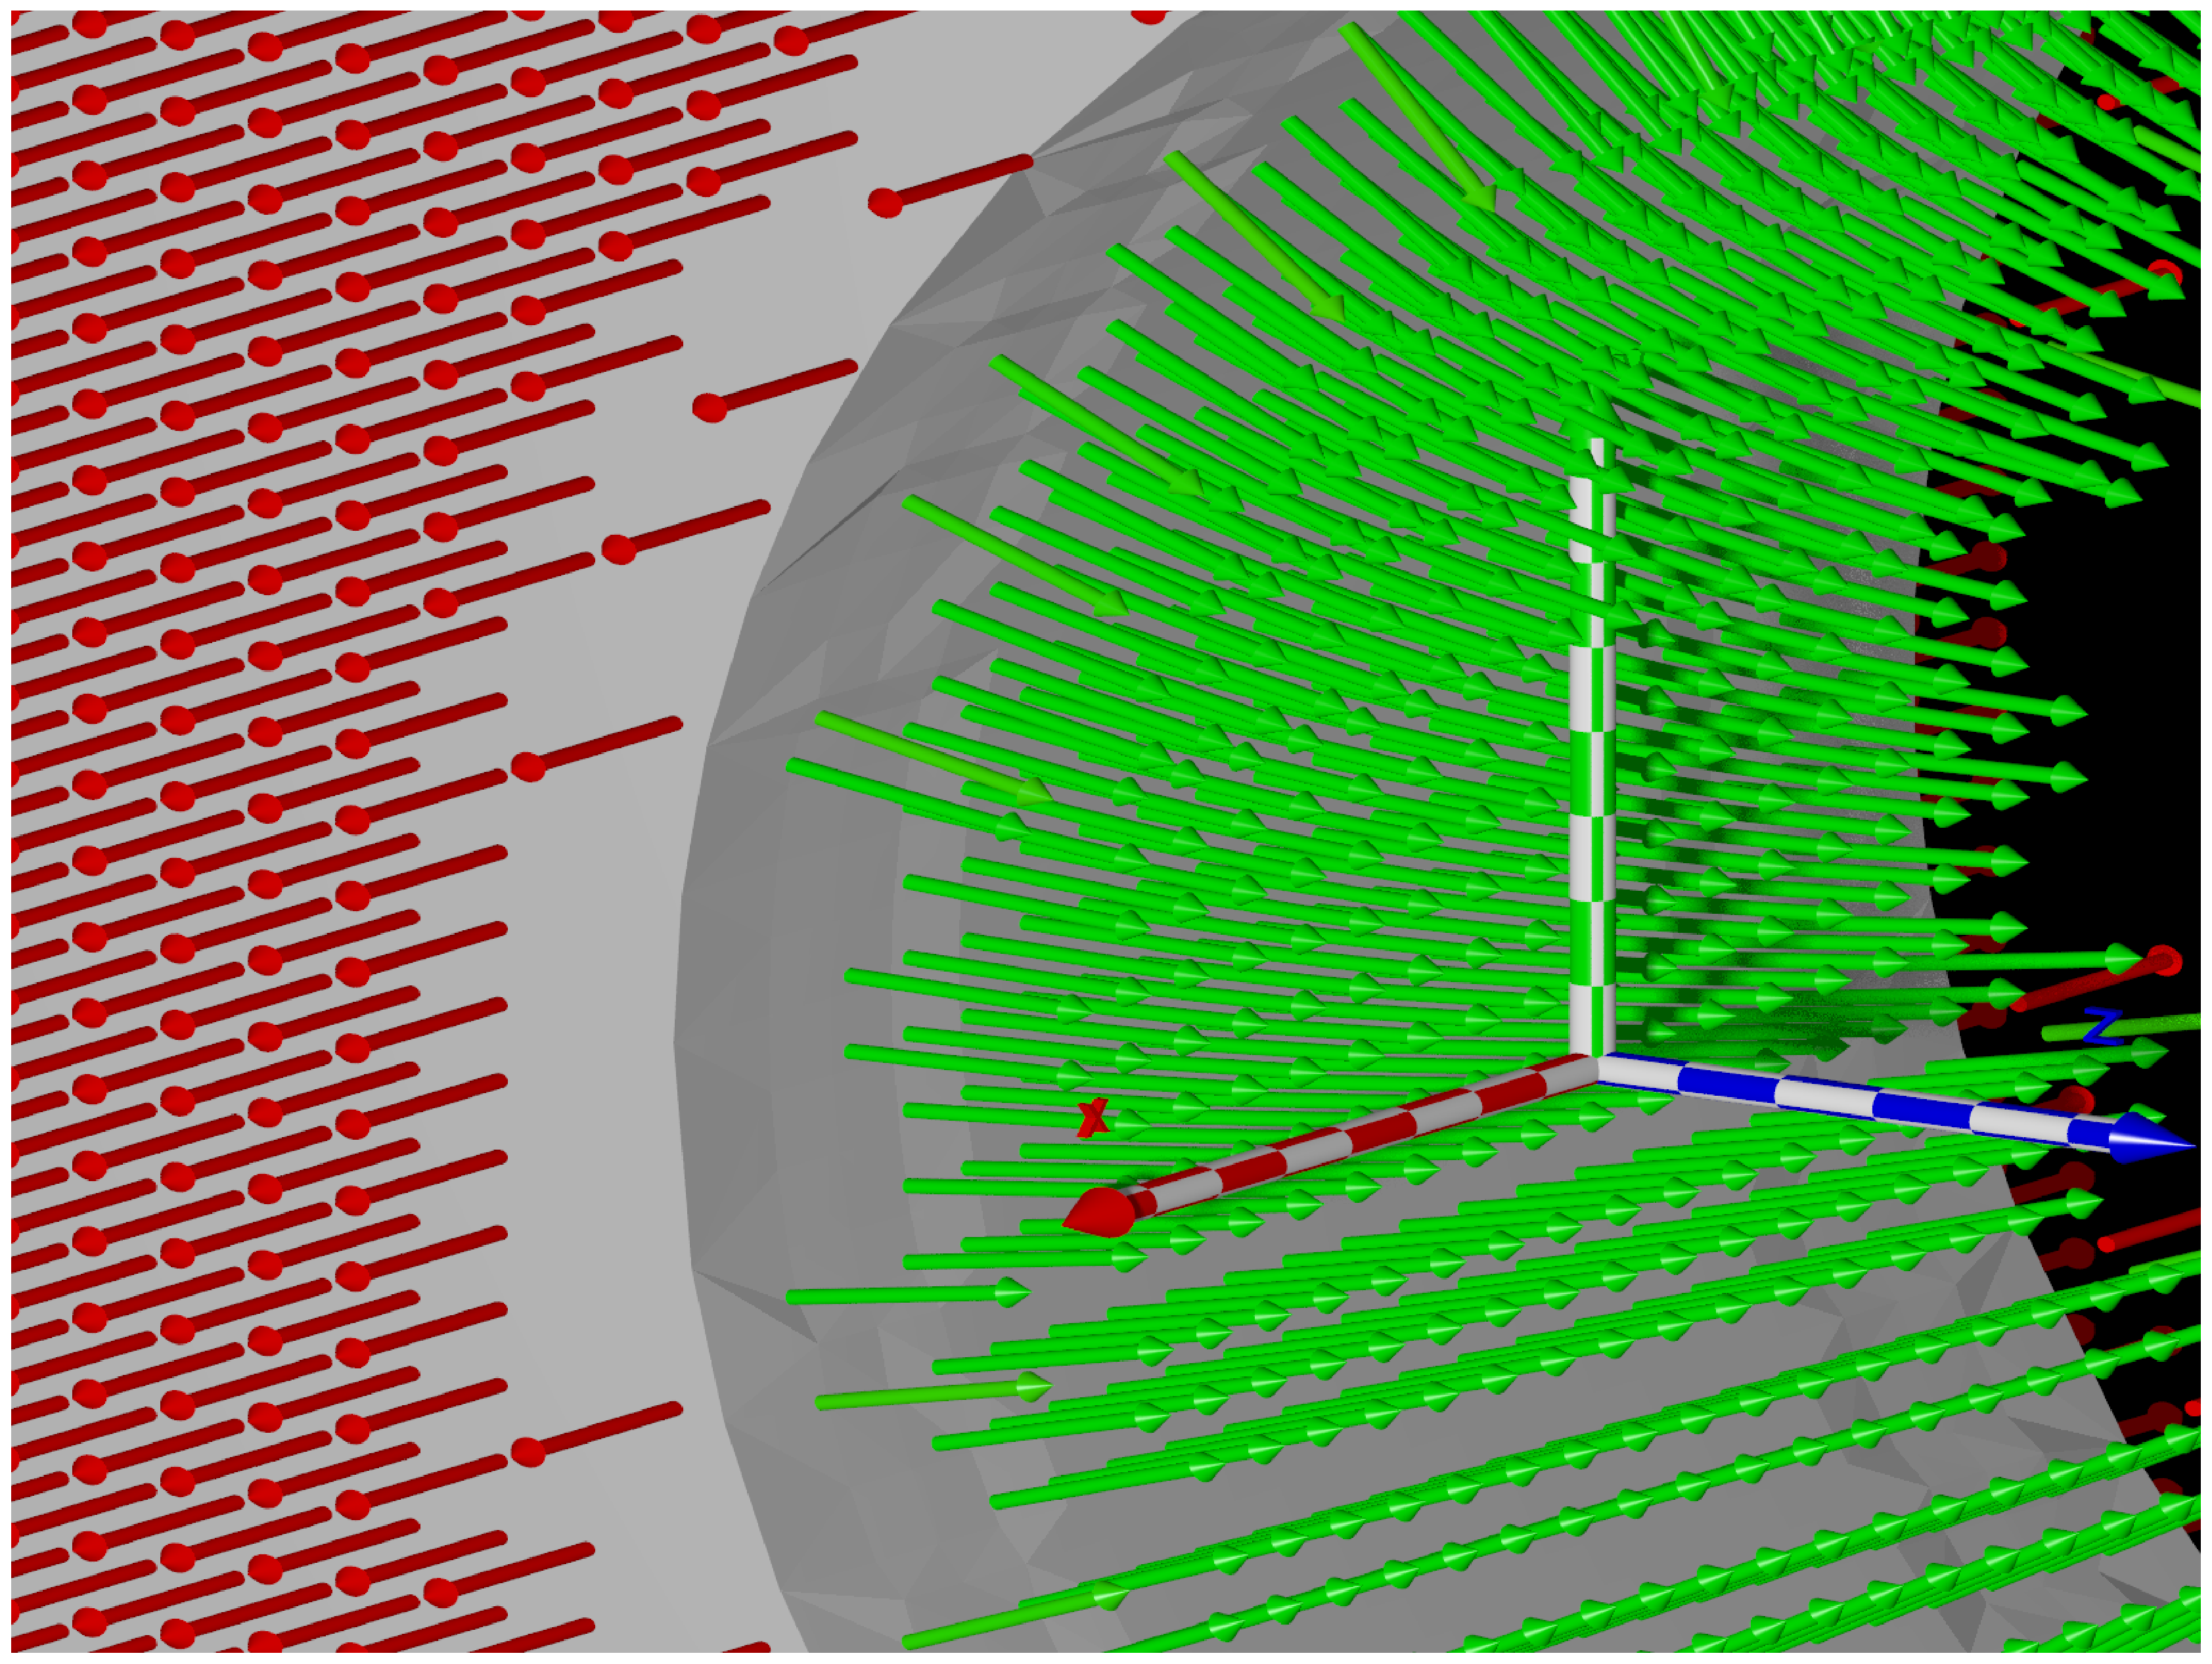
\includegraphics[width=0.3\linewidth]{images/annulus.gradcompare.algo1.eps}\label{fig:annulus:algo1} }\quad
    \subfloat[Edge dist. 2 predictions]{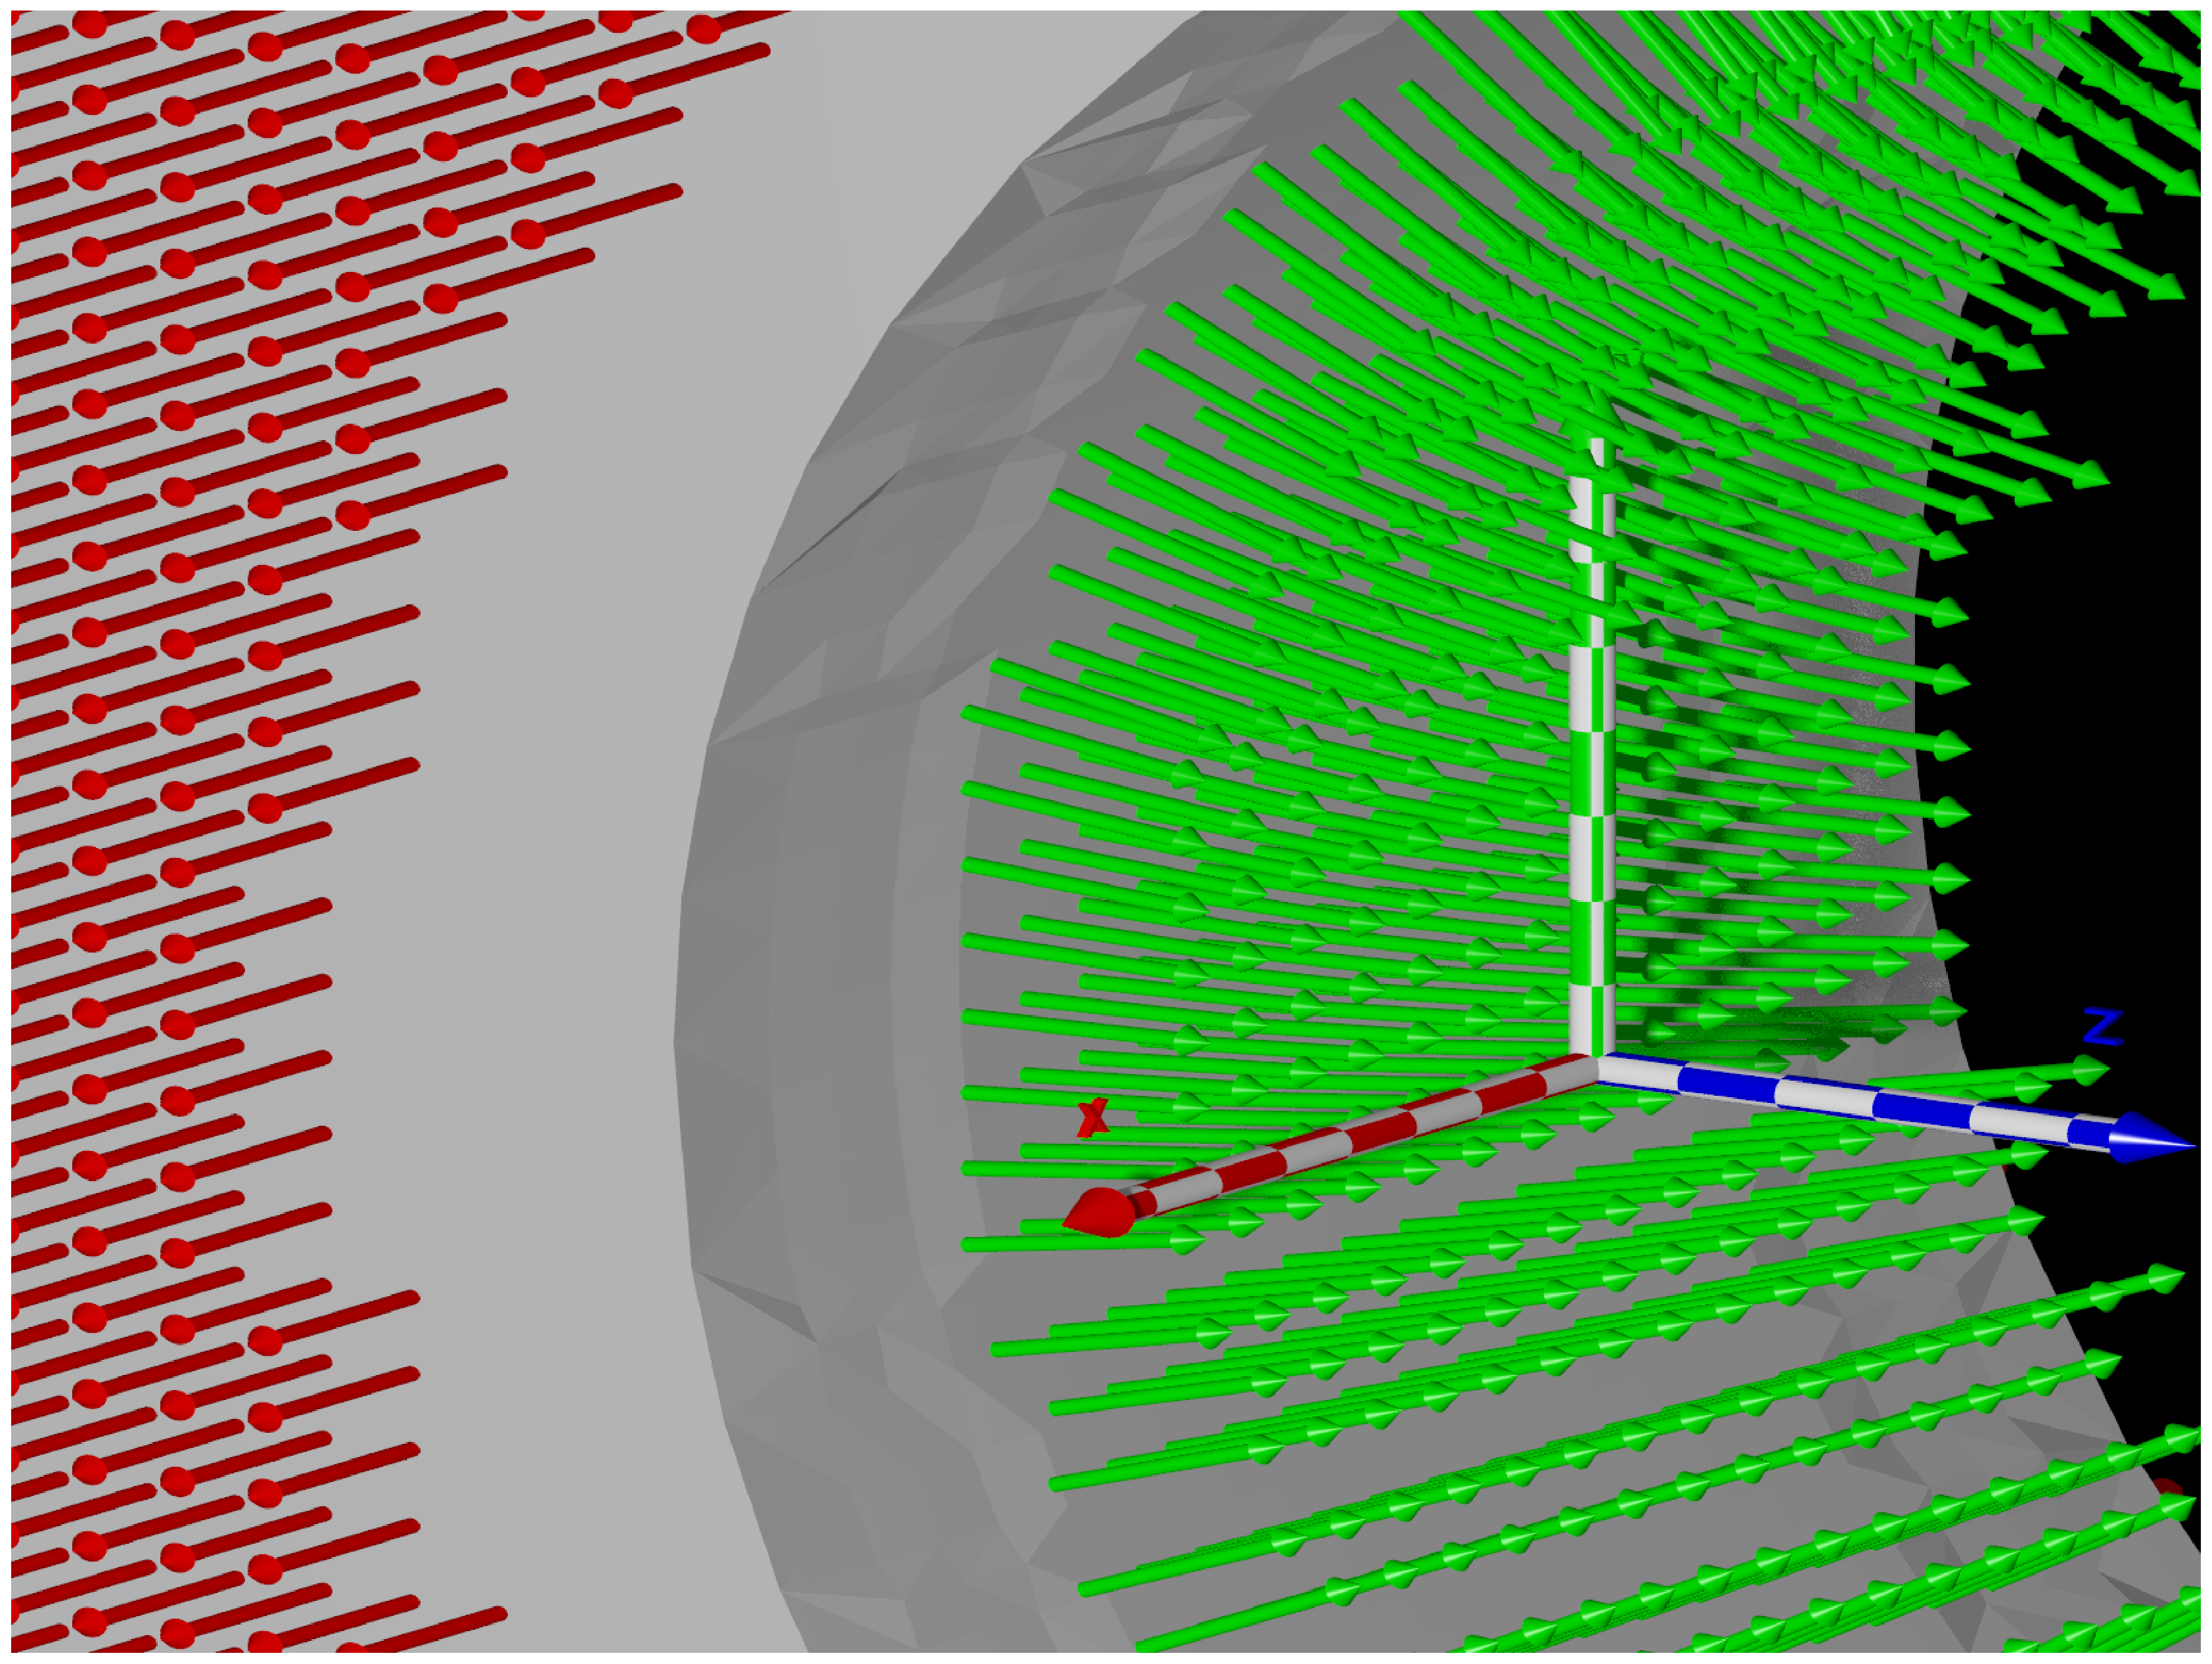
\includegraphics[width=0.3\linewidth]{images/annulus.gradcompare.algo2.eps}\label{fig:annulus:algo2}} \\\vspace{-4mm}
    \subfloat[Central Difference]{\includegraphics[width=0.45\linewidth]{images/gradCompare.full.A.eps}\label{fig:annulus:cdiff} }
    \subfloat[ReliGrad]
    {\includegraphics[width=0.45\linewidth]{images/gradCompare.full.B.eps}\label{fig:annulus:religrad} }\vspace{-3mm}
    \caption{Gradient results on a part of the \emph{Annulus} dataset (Figure~\protect\subref*{fig:annulus}).
     \protect\subref{fig:annulus:correct} Correct gradients.
     \protect\subref{fig:annulus:algo1}  Gradients marked correct by Algorithm 1 which uses $n_{v''}$ and $n_{v'}$ to predict $n_v$.
     \protect\subref{fig:annulus:algo2} Gradients marked correct by Algorithm 2 which uses $n_{v'''}$, $n_{v''}$, and $n_{v'}$ to predict $n_v$.
     \protect\subref{fig:annulus:cdiff} Central difference gradients. The blue inset on the right contains a magnified view. 
     \protect\subref{fig:annulus:religrad} Gradients marked correct by \protect\ReliGrad. The cyan inset shows a magnified view.
     }
    
\label{fig:annulus:gradResults}
\end{figure*}
\textbf{Reliable Gradients:}
Figure~\ref{fig:annulus:gradResults} shows gradients at grid vertices for grid cubes which intersect the isosurface on a zoomed in section of the \textit{Annulus} dataset.
To get the colormap for the gradient vectors, we projected all gradient vectors on to the XY plane, the angle of the resulting vector to the X-Axis is mapped between red-green. Gradients close to X-Axis are red, those perpendicular are green. 
Figure~\protect\subref*{fig:annulus:correct} shows the known correct gradients at all the grid vertices.  Figure~\subref*{fig:annulus:cdiff}, shows the central difference (CDiff) gradients at all the grid vertices. The blue inset shows a magnified view: CDiff gradients are inaccurate along discontinuities, compared to the known correct gradients (figure~\subref*{fig:annulus:correct}).  Figure~\subref*{fig:annulus:algo1} shows gradients only at vertices marked correct by Algorithm 1. Algorithm 1  which uses $n_{v''}$ and $n_{v'}$ to predict $n_v$. Figure~\protect\subref*{fig:annulus:algo2} shows results from Algorithm 2, which uses $n_{v'''}$, $n_{v''}$, and $n_{v'}$ to predict $n_v$. 
Algorithm 1 does not handle curved boundaries and vertices close to the discontinuity are marked correct. Figure~\subref*{fig:annulus:religrad} shows gradients marked reliable by \protect\ReliGrad, the cyan inset shows a close-up, the inaccurate gradients are marked unreliable  by \ReliGrad and not shown. 

% %Cannon
\begin{figure}
    \centering
    \subfloat[Correct gradients]{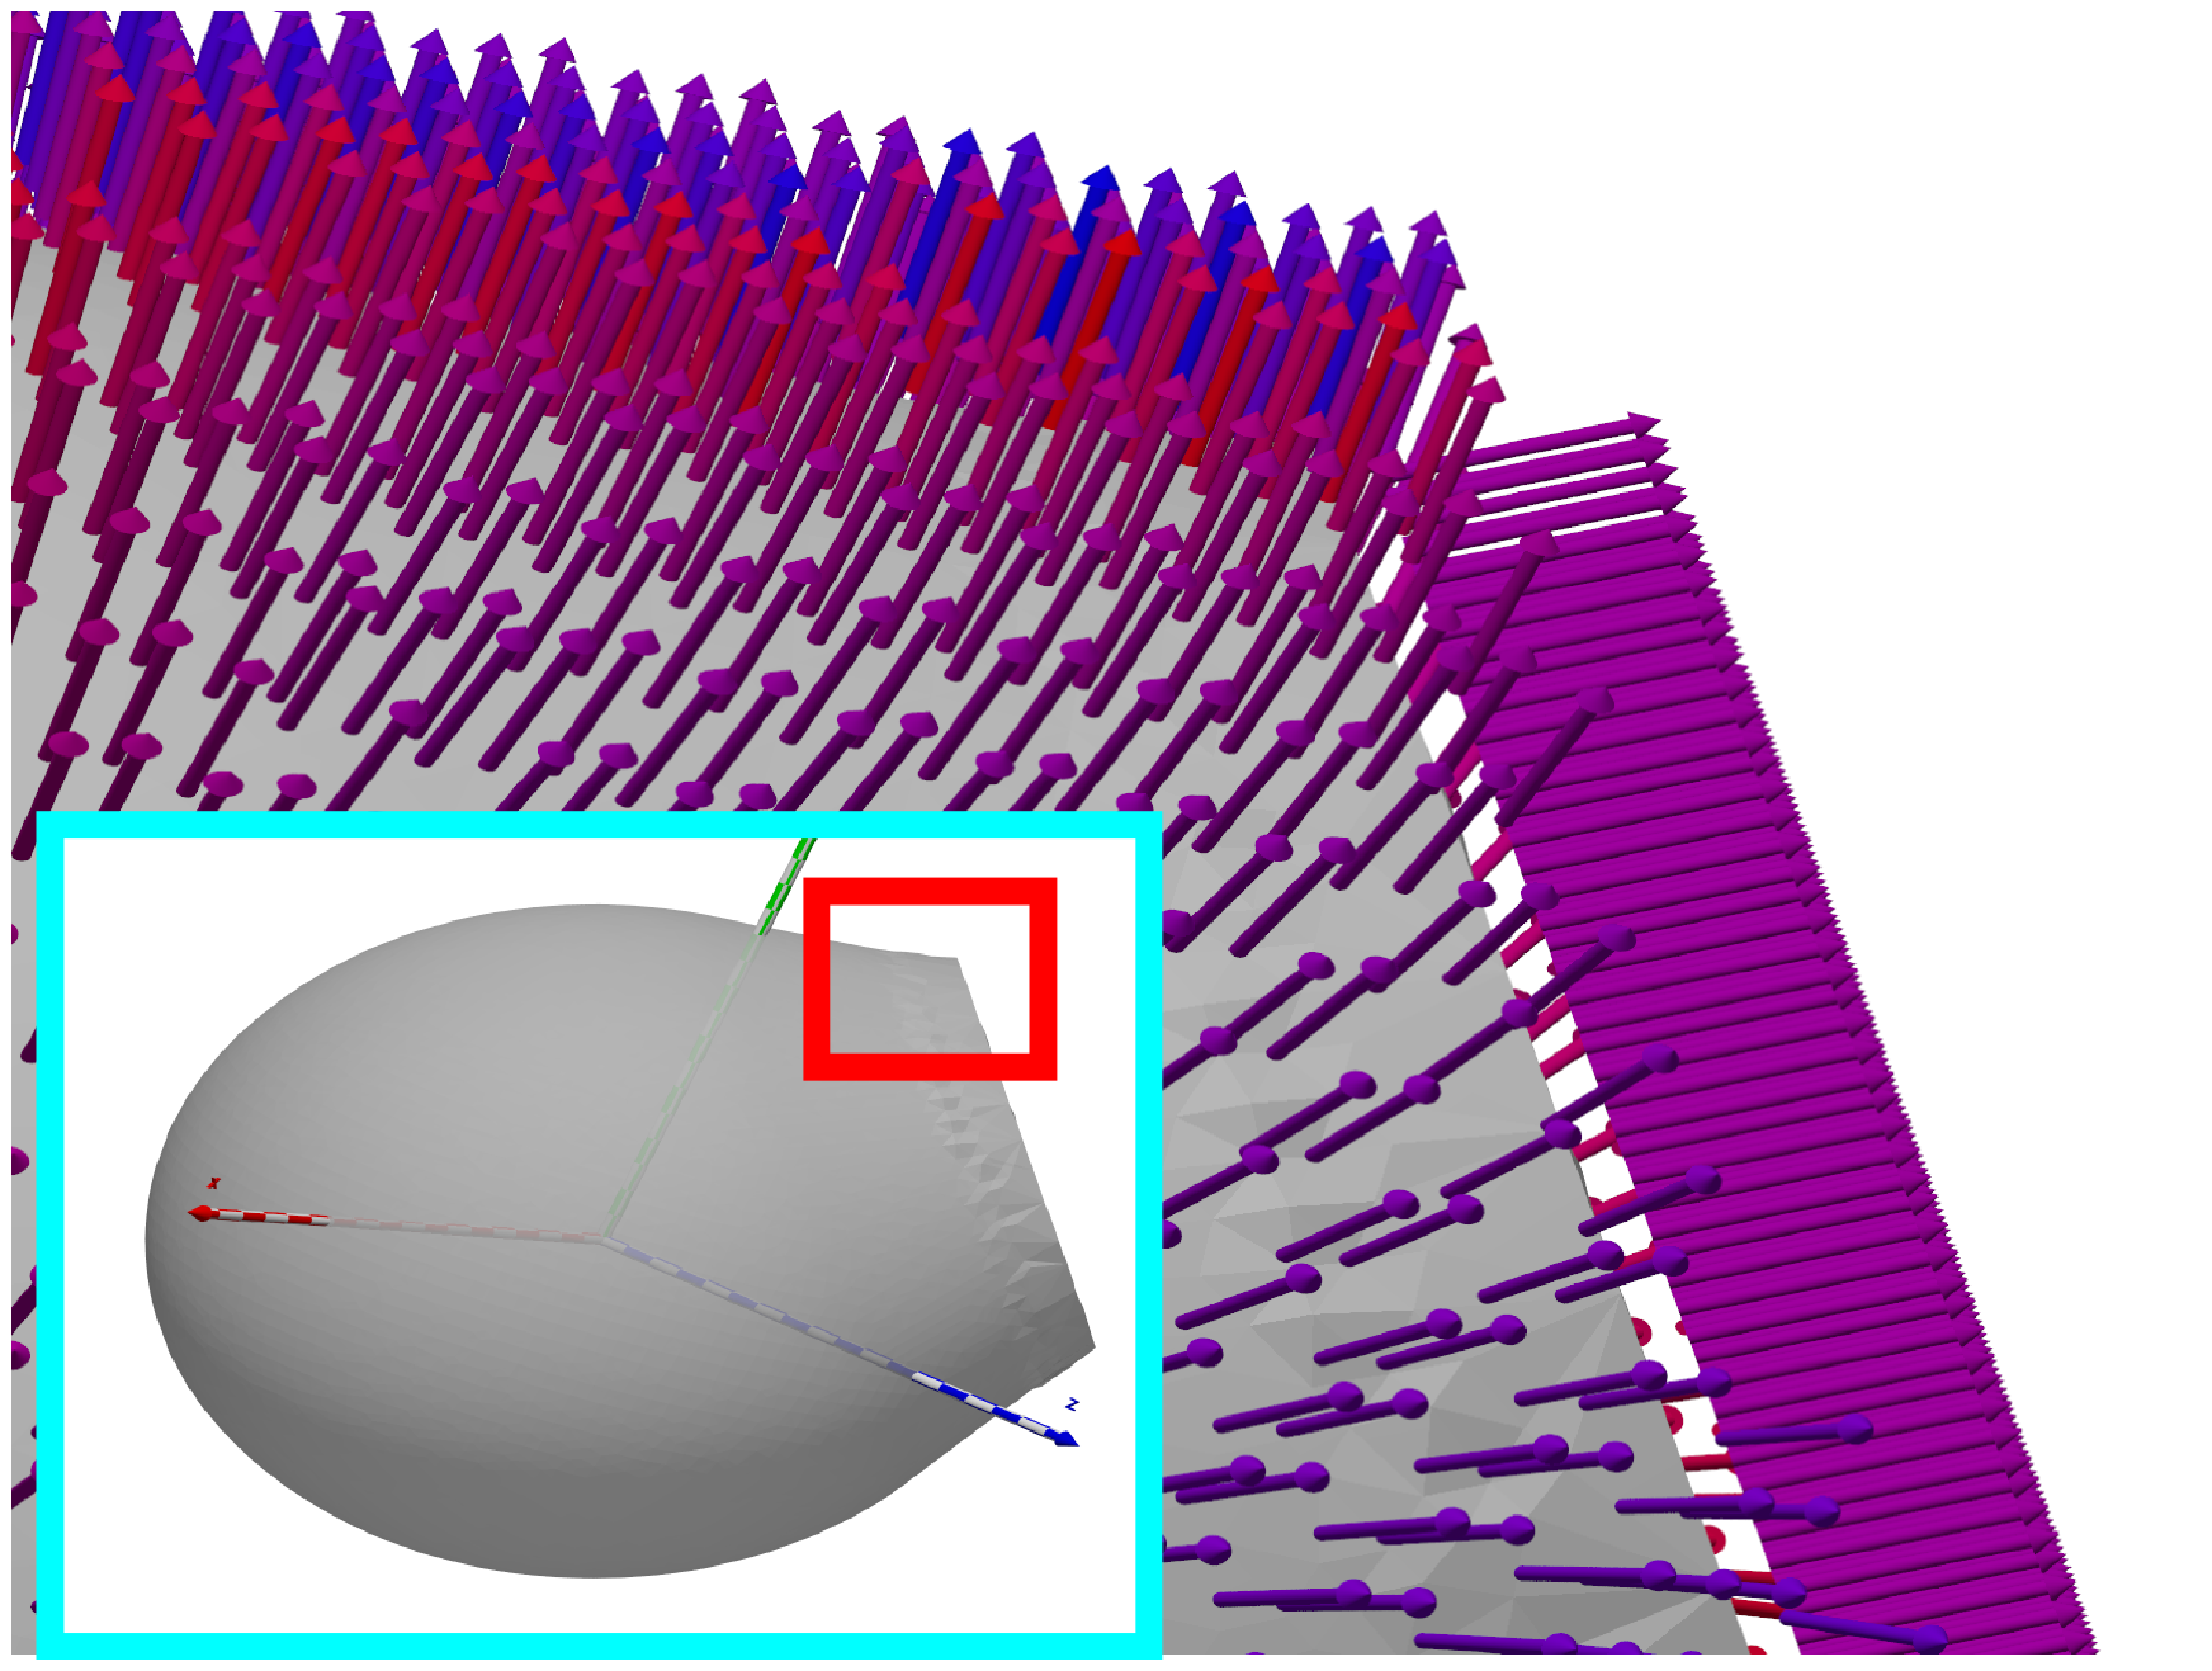
\includegraphics[width=0.5\linewidth]
        {images/cannon.correct.close.eps}\label{fig:cannon.correct}}
    \subfloat[CDiff gradients]{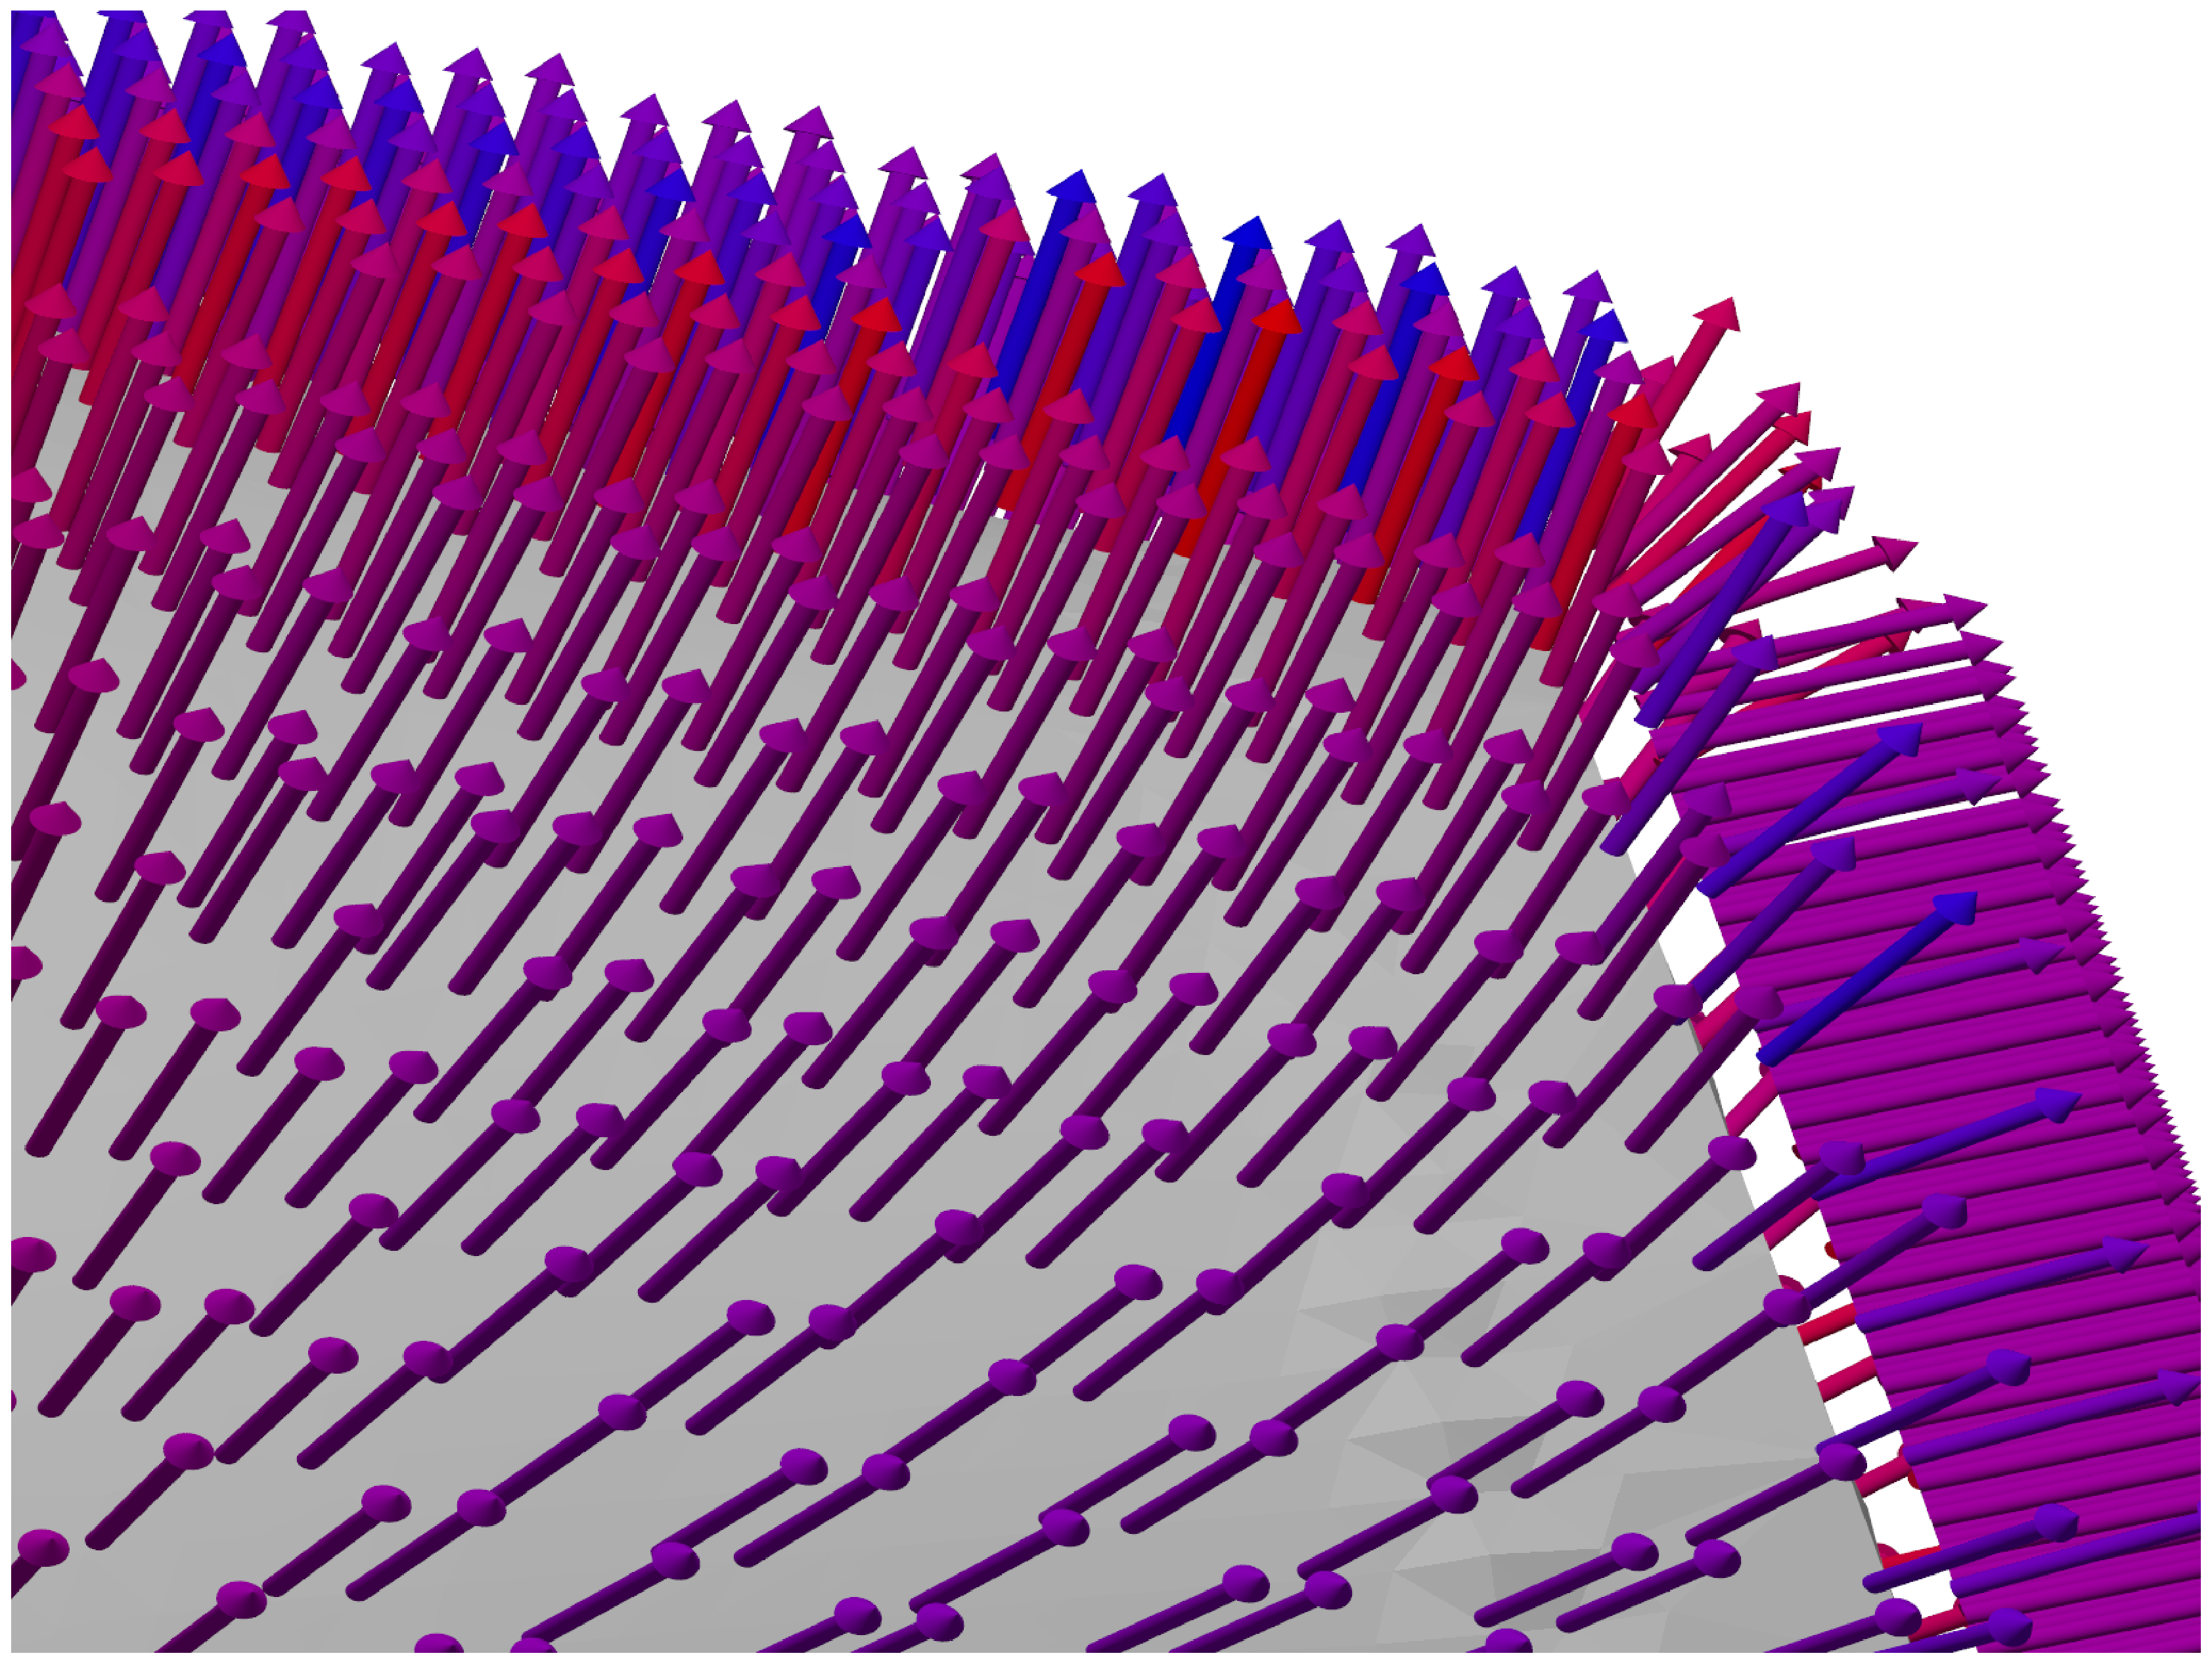
\includegraphics[width=0.5\linewidth]
        {images/cannon.cdiff.close.eps}\label{fig:cannon.cdiff}}\hspace{1mm}  
    \\   \vspace{-3mm}
    \subfloat[FindReliable gradients]{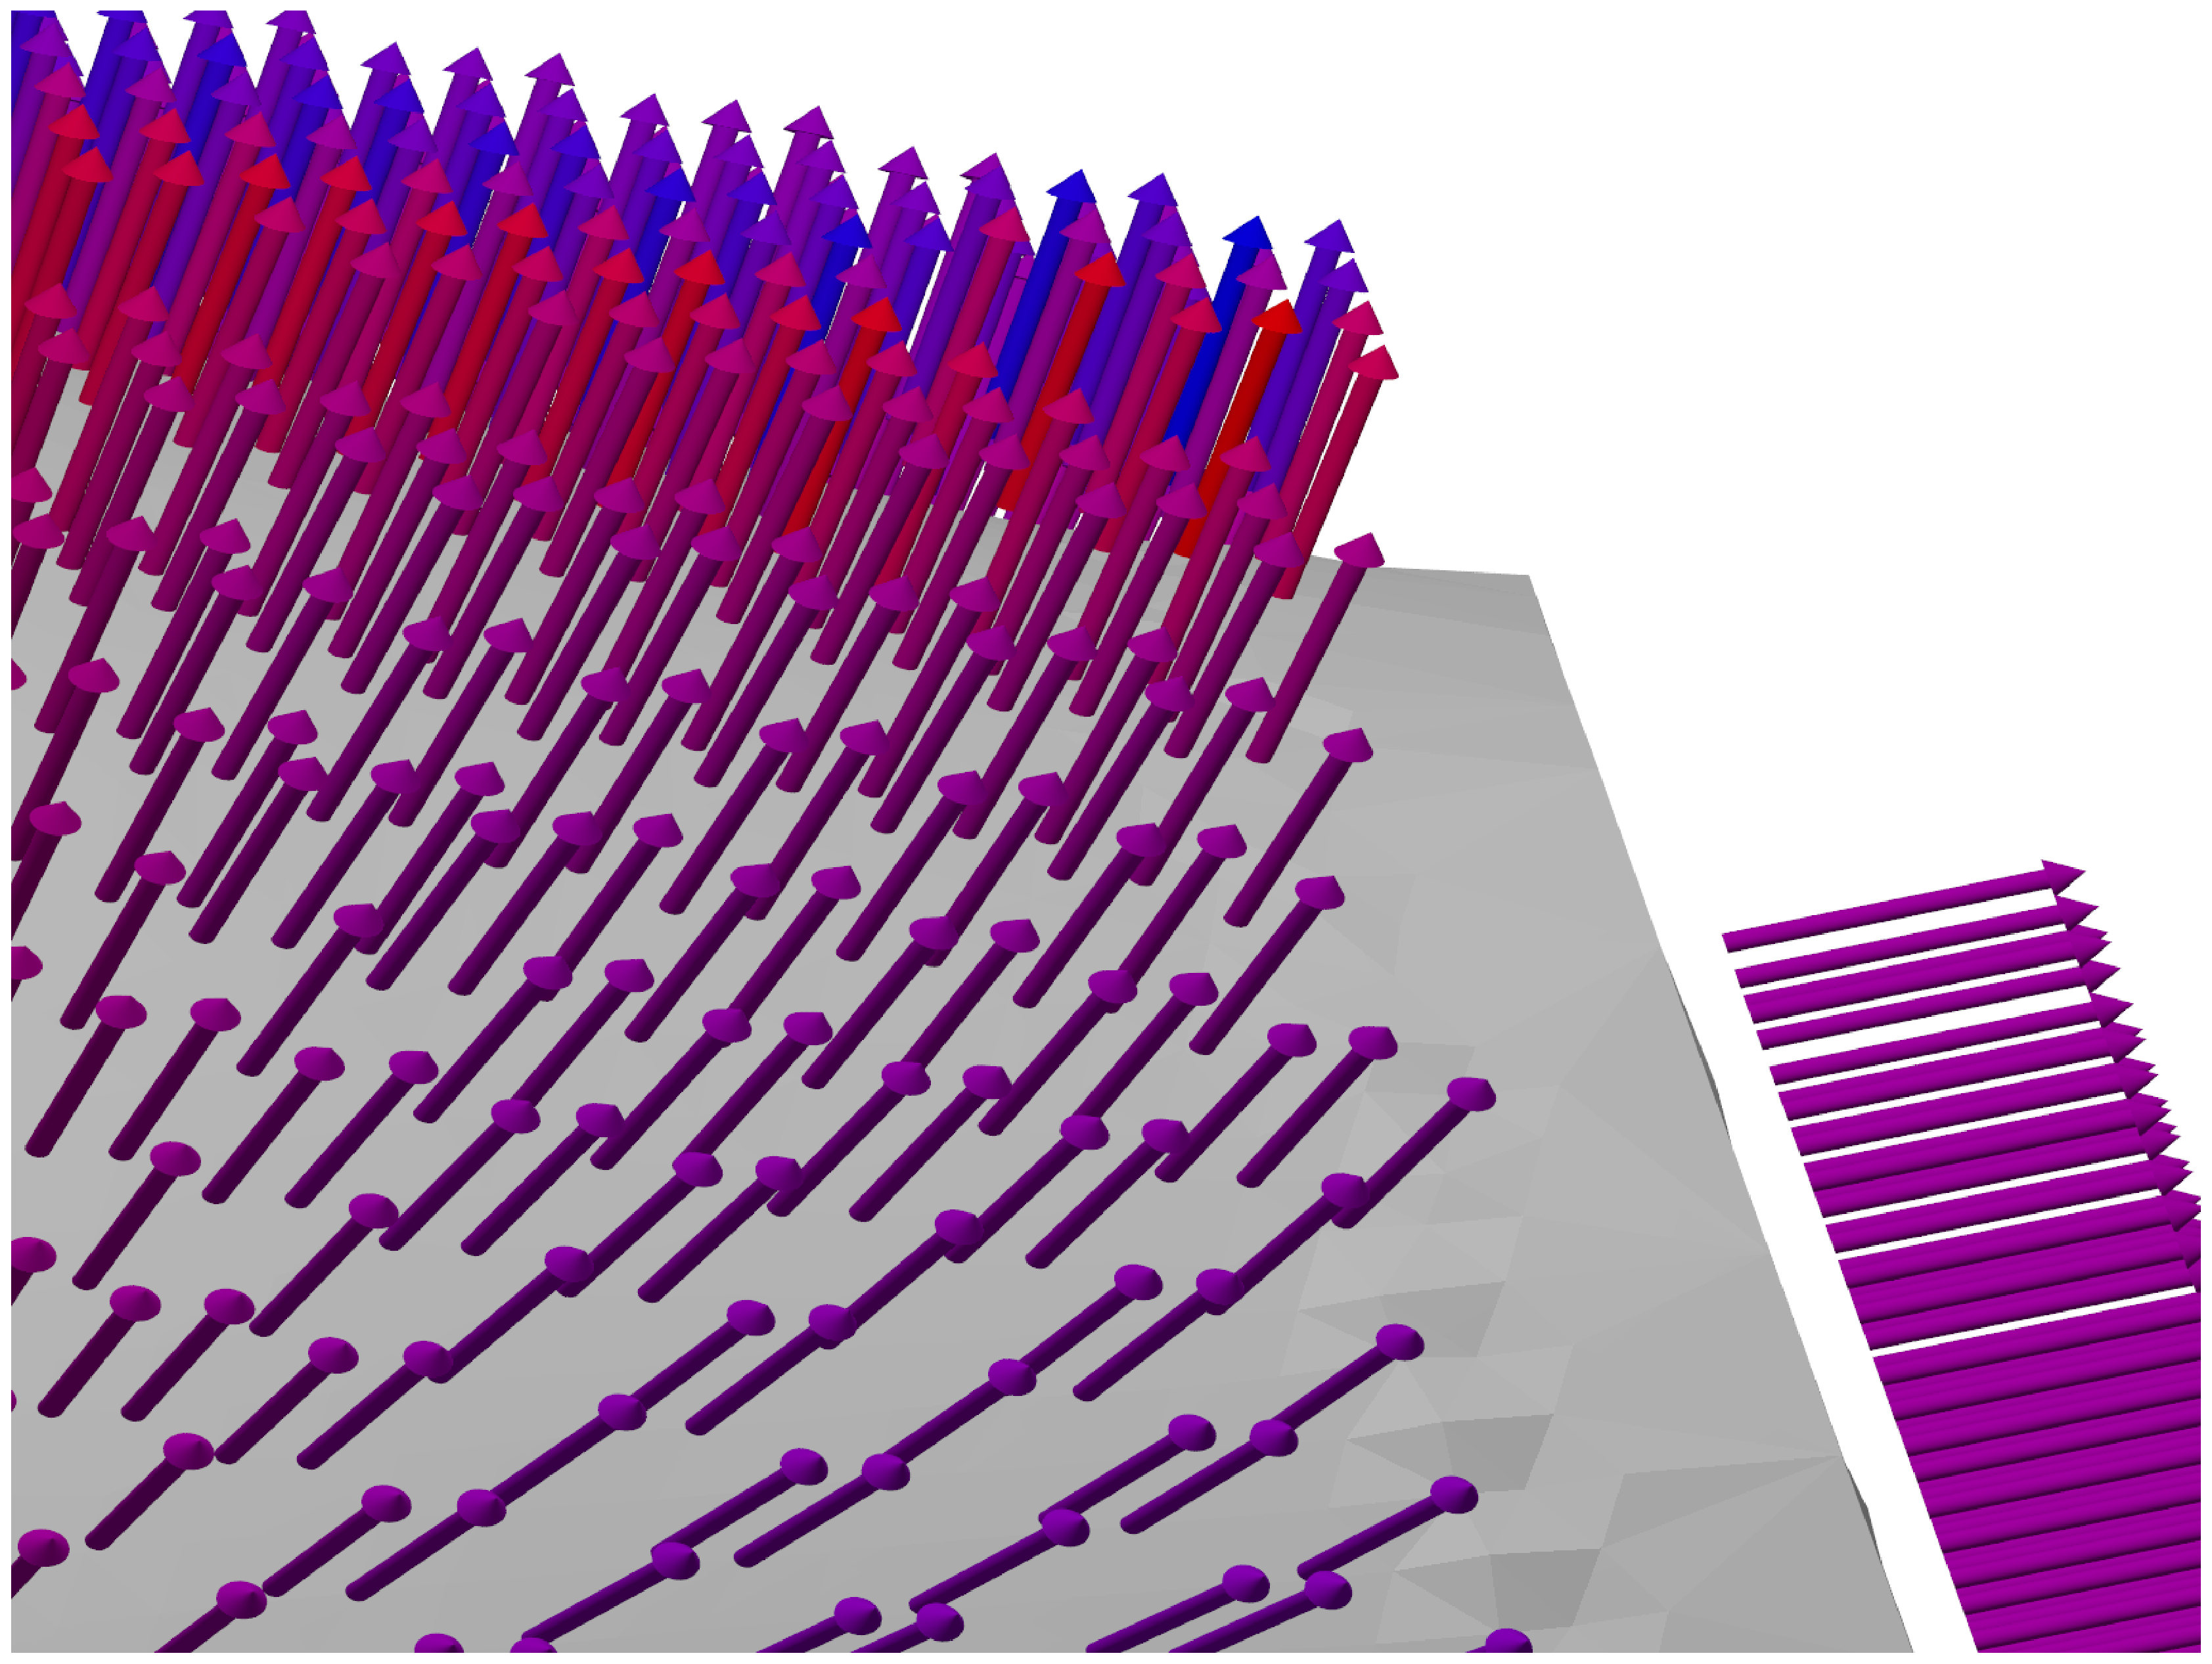
\includegraphics[width=0.45\linewidth]
        {images/cannon.findreliable.close.eps}\label{fig:cannon.findreliable}}
    \subfloat[Religrad gradients]{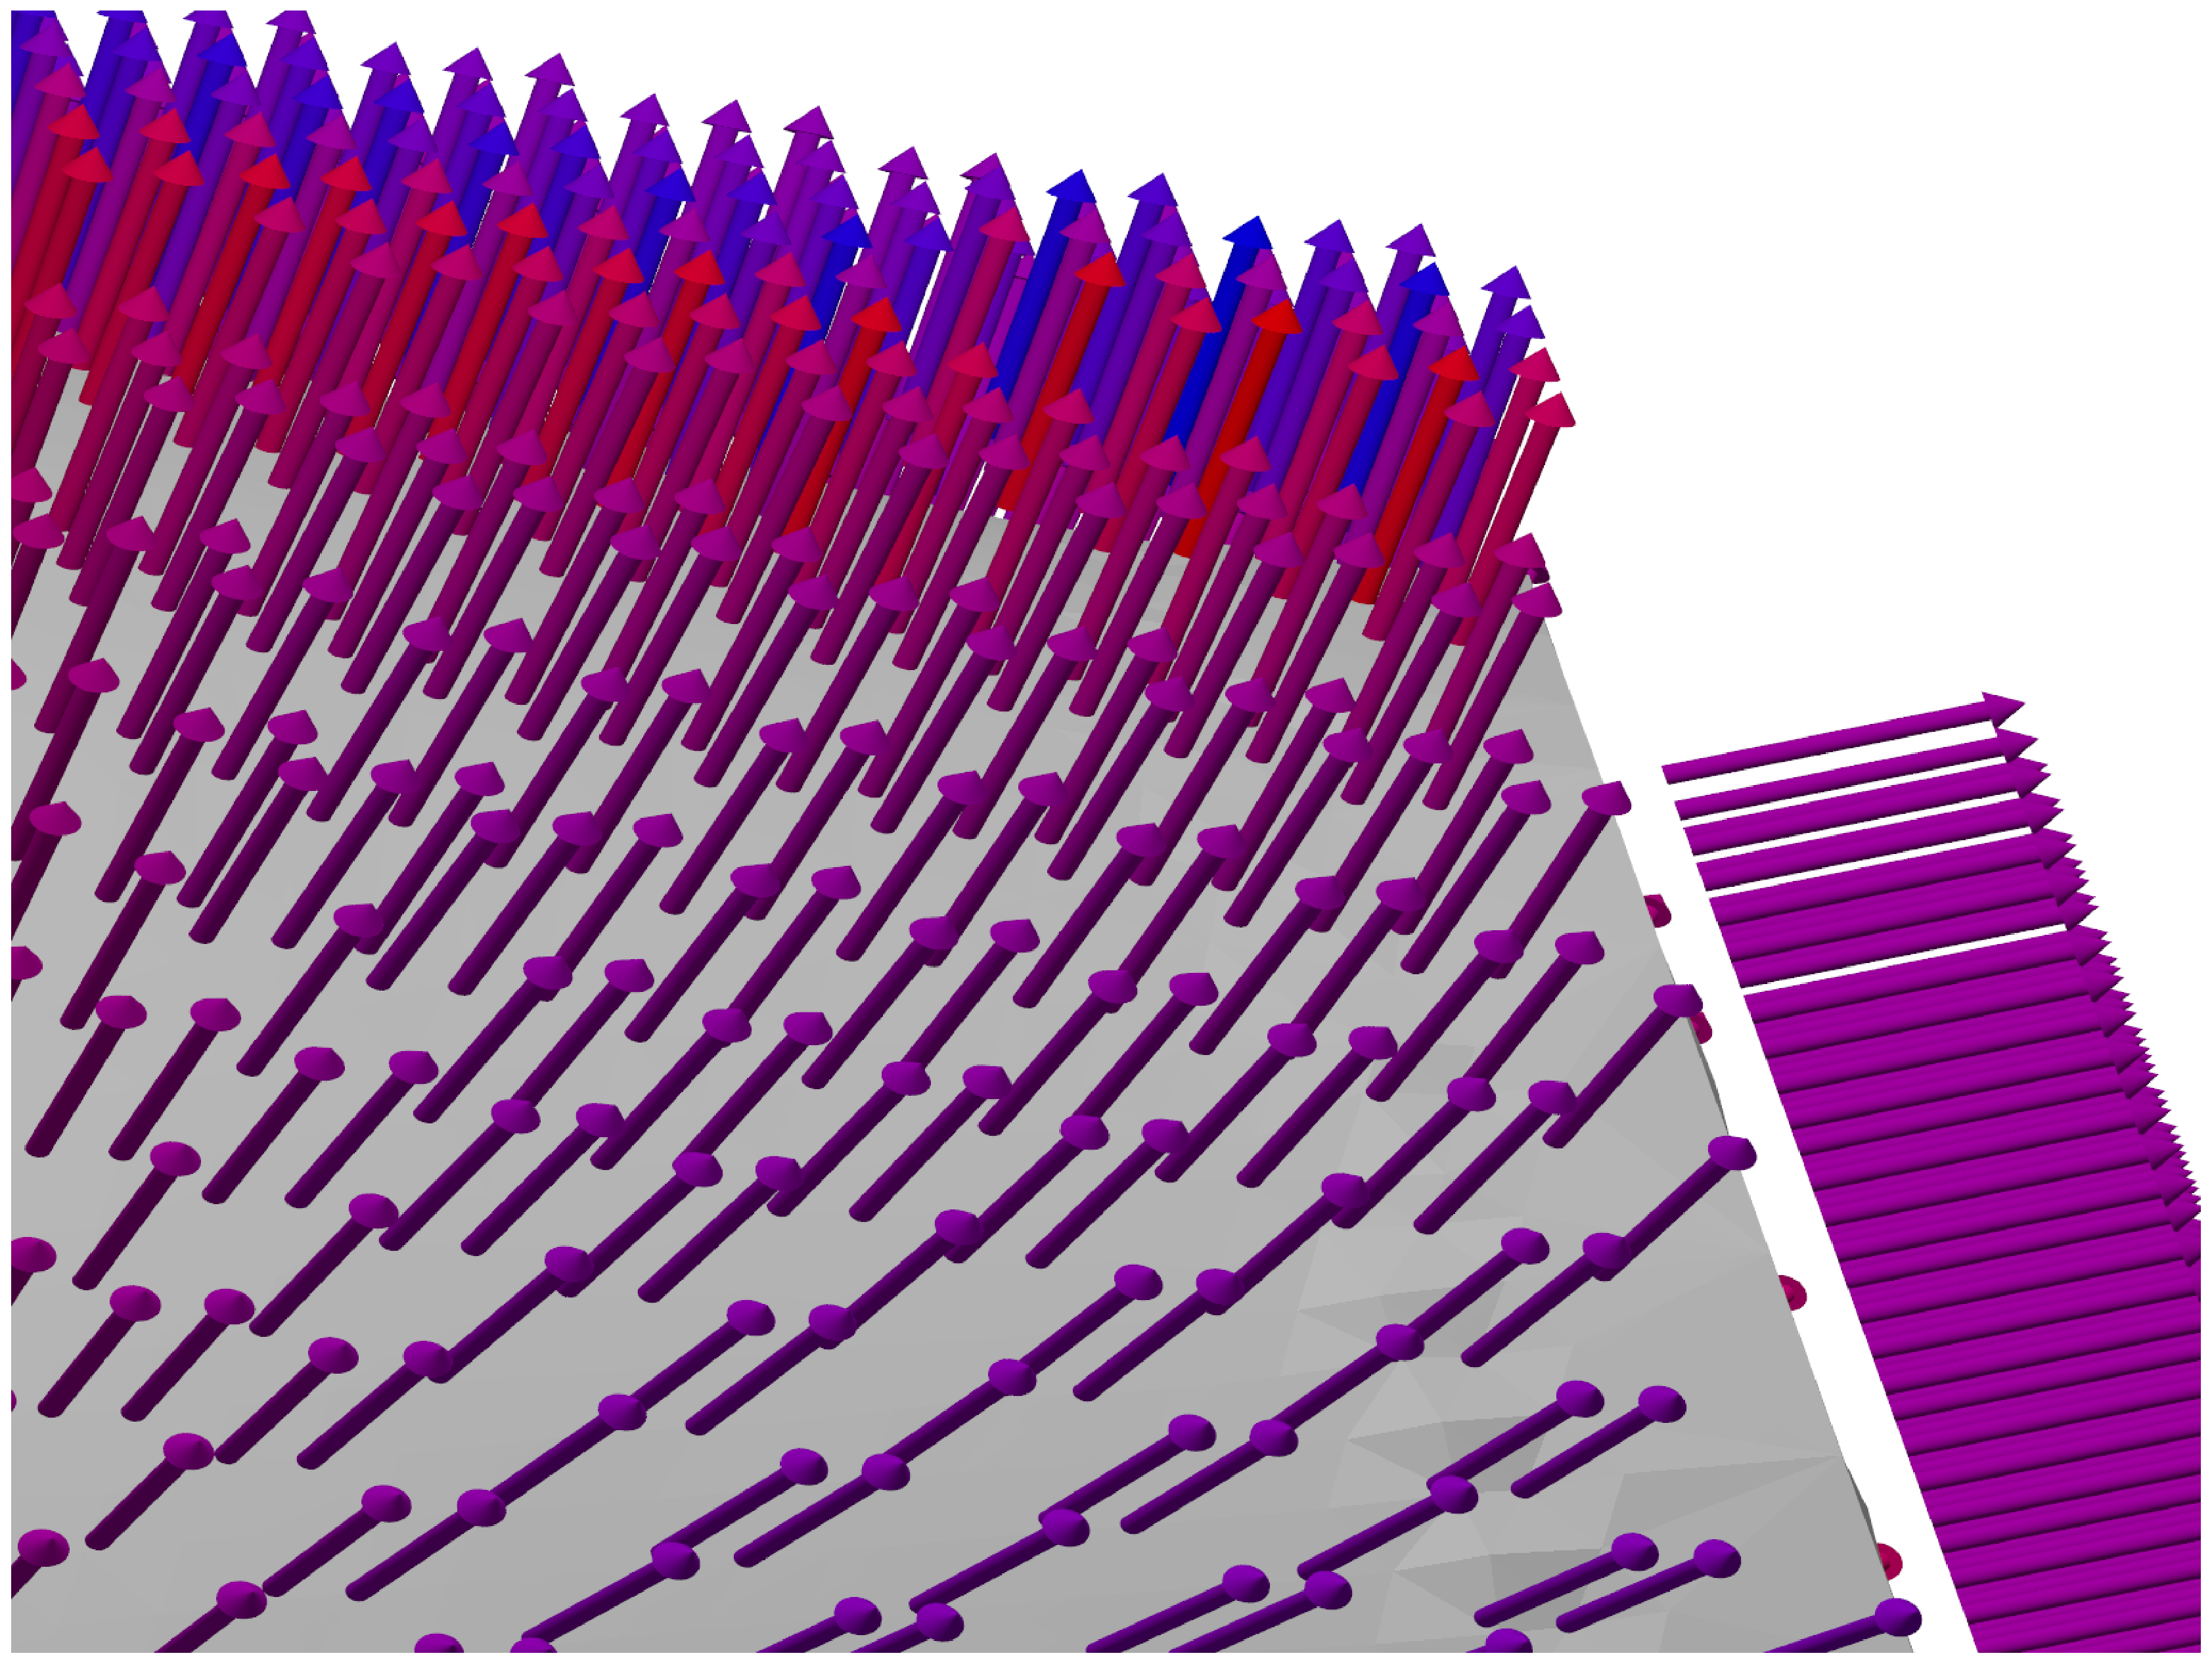
\includegraphics[width=0.45\linewidth]
        {images/cannon.religrad.close.eps}\label{fig:cannon.religrad}}\vspace{-3mm}
    \caption{Cannon dataset gradients (Curved edge, non 90$^\circ$ angles). \protect\subref{fig:cannon.correct} correct gradients, \protect\subref{fig:cannon.cdiff} central difference gradients, \protect\subref{fig:cannon.findreliable} gradients marked correct by FindReliable. \protect\subref{fig:cannon.religrad}  gradients at grid vertices marked correct by \protect\ReliGrad. Inaccurate CDiff gradients \protect\subref{fig:cannon.cdiff} across the discontinuity are not marked correct, hence not shown.}
    \label{fig:cannon:gradients}
\end{figure}


%\begin{figure*}
%    \centering
%    \subfloat[Correct gradients]{\includegraphics[width=0.25\linewidth]
%        {images/cannon.correct.close.eps}\label{fig:cannon.correct}}
%    \subfloat[CDiff gradients]{\includegraphics[width=0.24\linewidth]
%        {images/cannon.cdiff.close.eps}\label{fig:cannon.cdiff}}\hspace{1mm}     
%    \subfloat[FindReliable gradients]{\includegraphics[width=0.24\linewidth]
%        {images/cannon.findreliable.close.eps}\label{fig:cannon.findreliable}}
%      \hspace{1mm}  
%    \subfloat[Religrad gradients]{\includegraphics[width=0.24\linewidth]
%        {images/cannon.religrad.close.eps}\label{fig:cannon.religrad}}
%    \caption{Cannon dataset gradients (Curved edge, non 90$^\circ$ angles). \protect\subref{fig:cannon.correct} correct gradients, \protect\subref{fig:cannon.cdiff} central difference gradients, \protect\subref{fig:cannon.findreliable} gradients marked correct by FindReliable. \protect\subref{fig:cannon.religrad}  gradients at grid vertices marked correct by \protect\ReliGrad. Inaccurate CDiff gradients \protect\subref{fig:cannon.cdiff} across the discontinuity are not marked correct, hence not shown.}
%    \label{fig:cannon:gradients}
%\end{figure*}
Figure~\ref{fig:cannon:gradients} shows the gradients around the edge of the \textit{Cannon} dataset (figure~\subref*{fig:cannon.correct} red rectangle shows the location). The dataset is not axis-parallel, the angle around the curved edge is not perpendicular. Figure~\subref*{fig:cannon.correct} shows known correct gradients at grid vertices which are intersected by the isosurface. Figure~\subref*{fig:cannon.cdiff} shows the central difference  gradients, at grid vertices of the intersected cubes. Note that along the discontinuity the central difference gradients are inaccurate compared to the correct gradients (figure~\subref*{fig:cannon.correct}). Figure~\subref*{fig:cannon.findreliable} shows gradients at grid vertices marked reliable by \FindReliable. Figure~\subref*{fig:cannon.religrad} shows gradients marked correct by \ReliGrad.
\begin{figure}[ht]
    \centering
    \subfloat[]{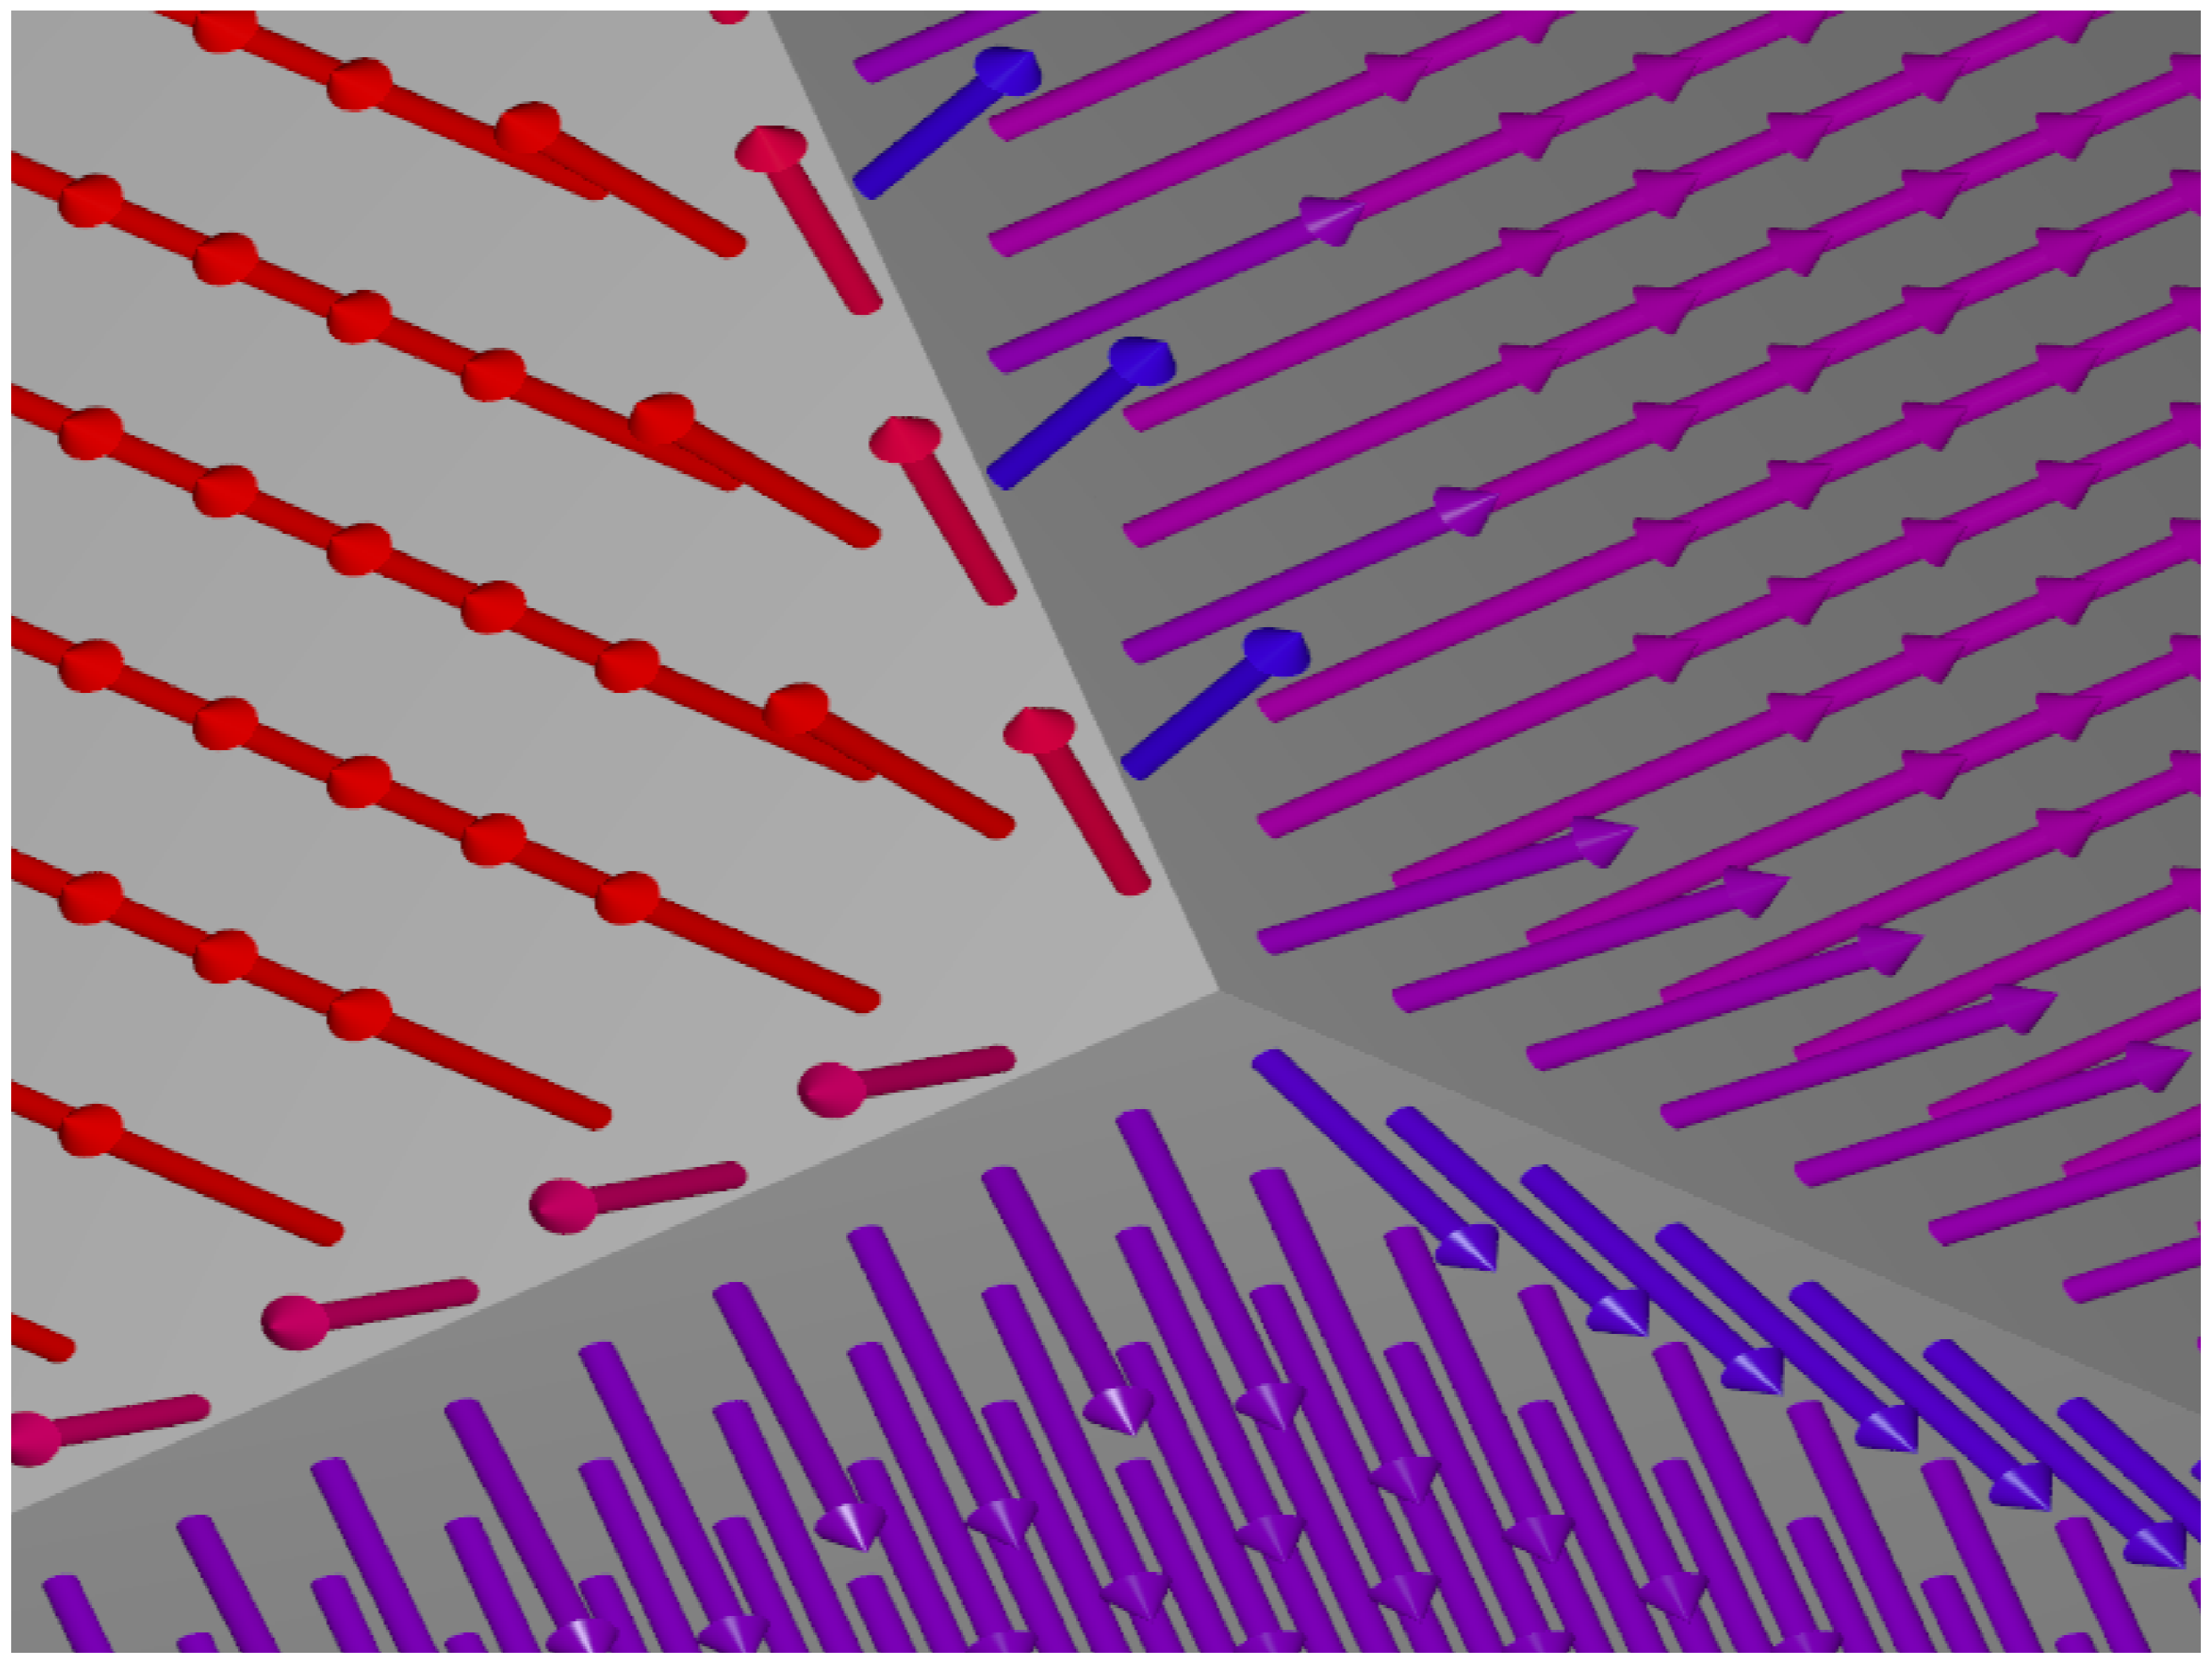
\includegraphics[width=0.25\linewidth]{images/cube.cdiff.eps}\label{fig:cube:cdiff}}
    \subfloat[]{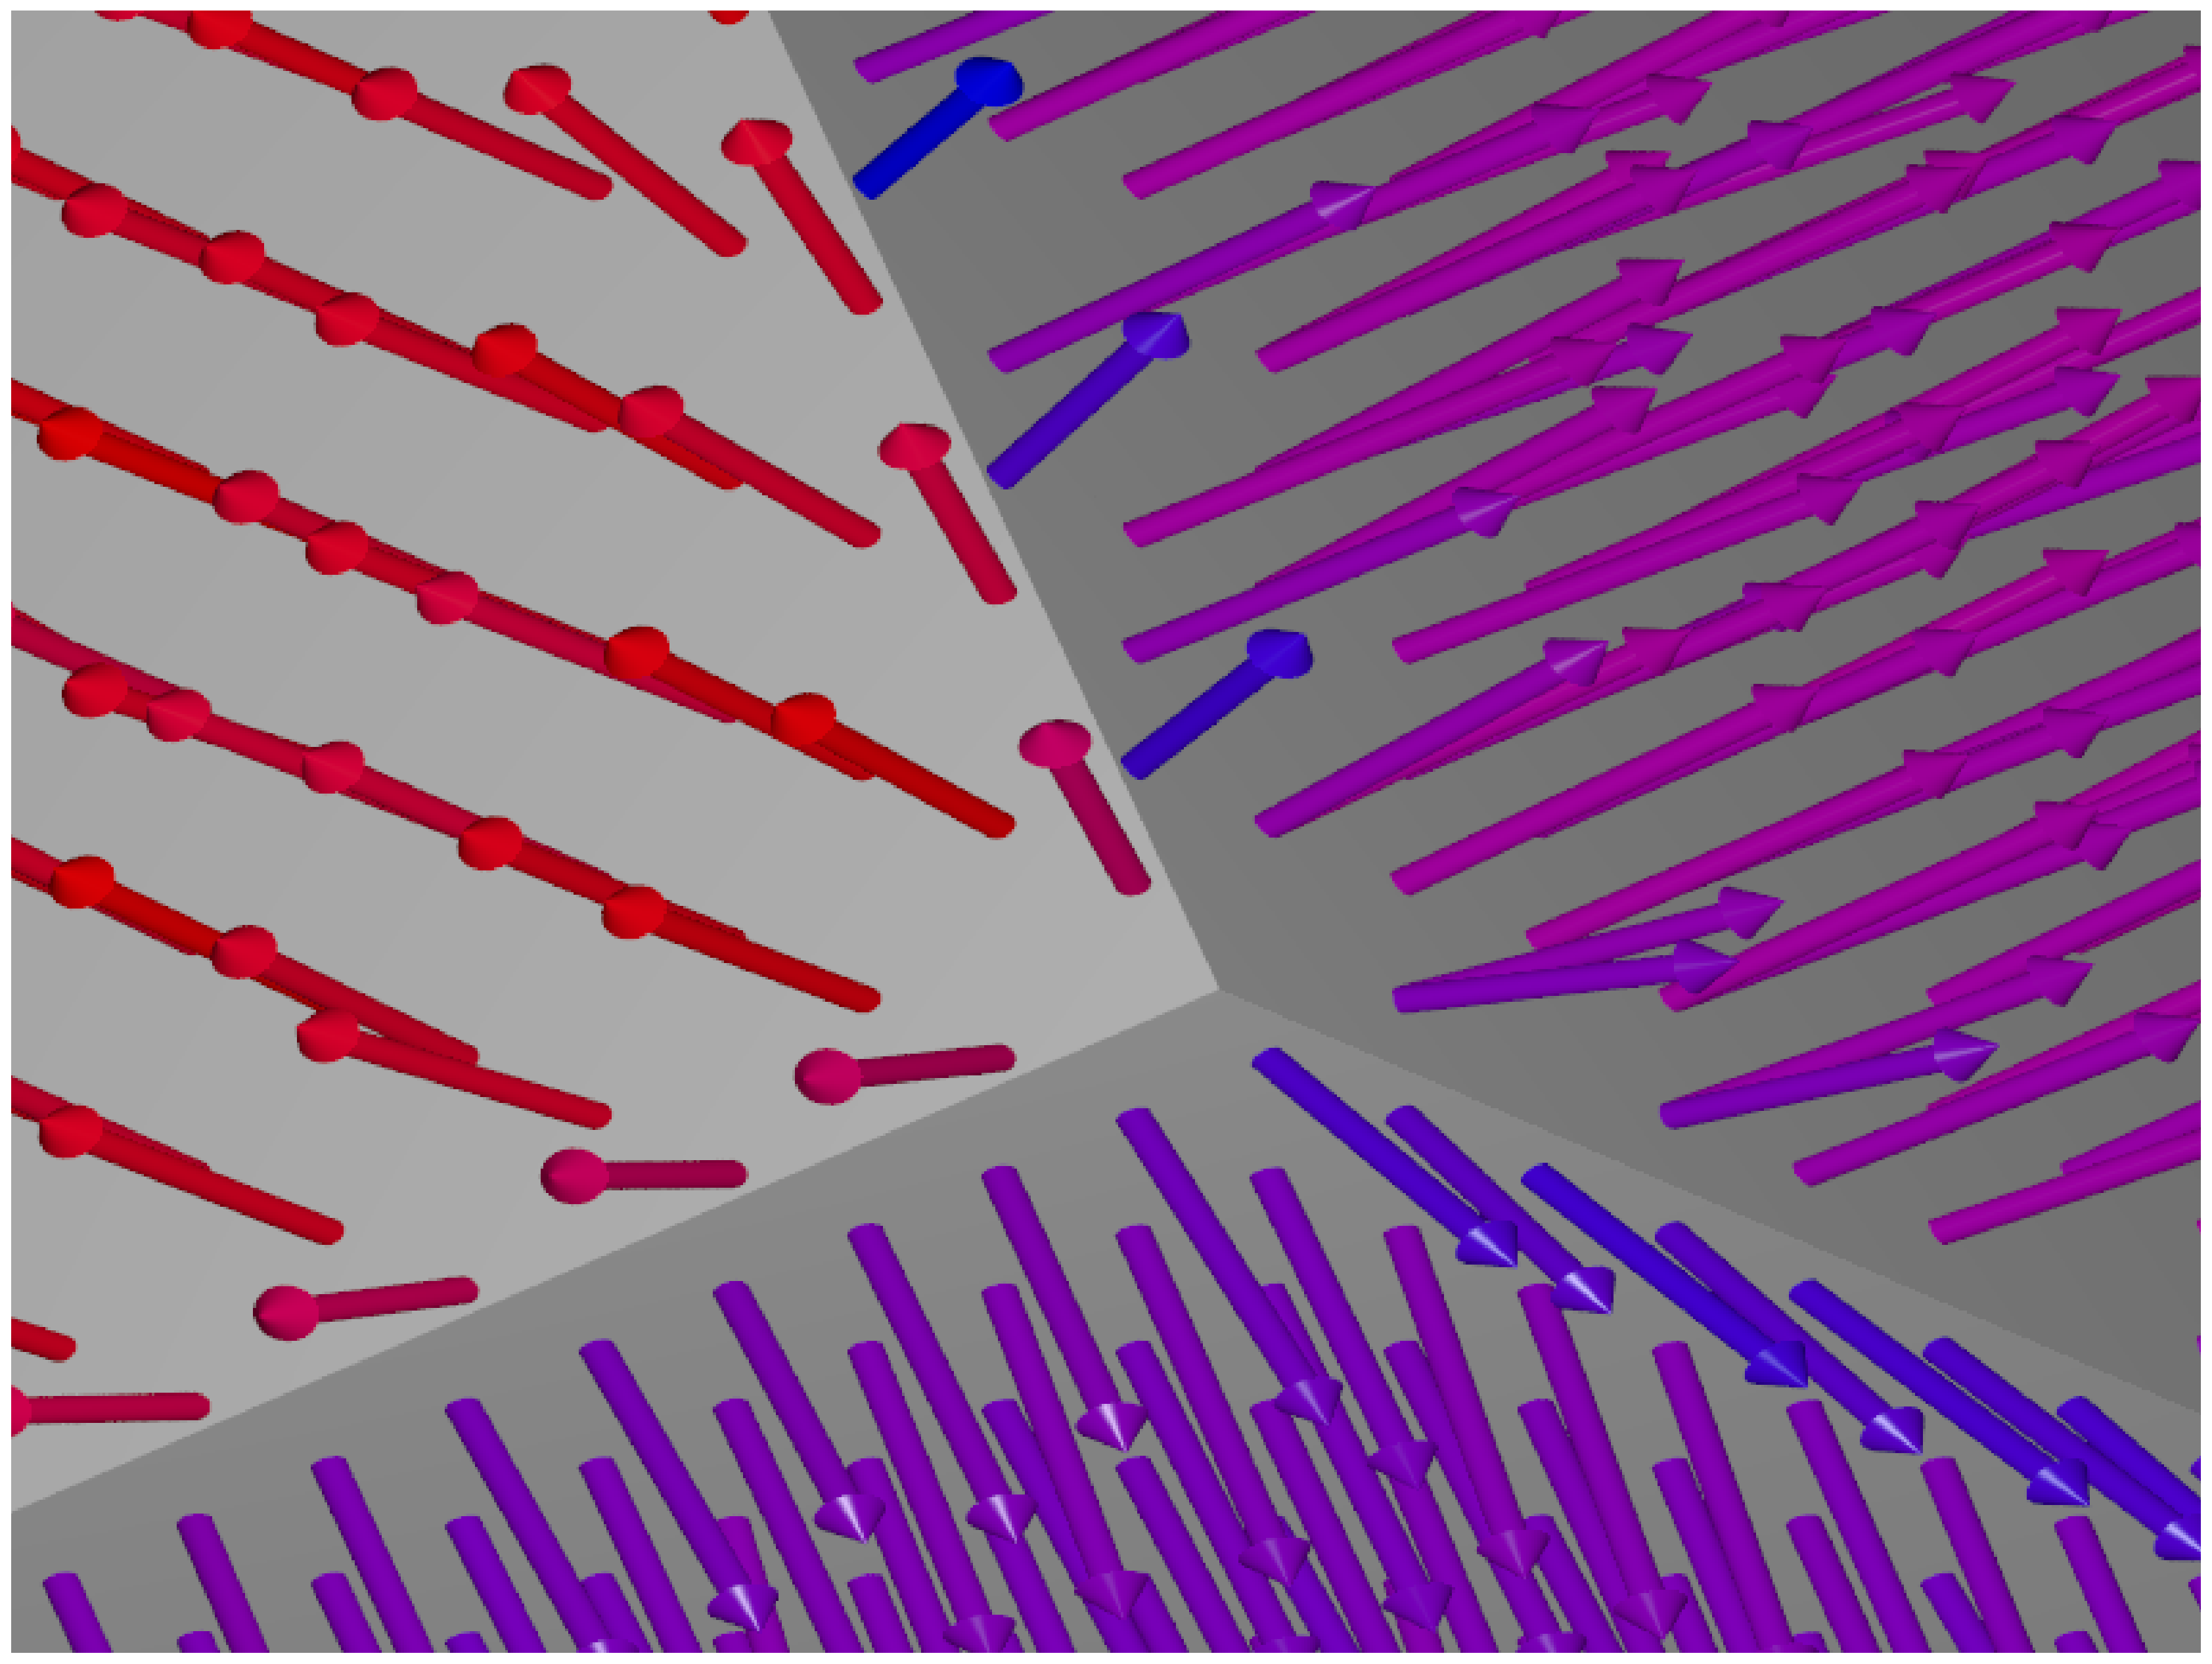
\includegraphics[width=0.25\linewidth]{images/cube.noise.cdiff.eps}\label{fig:cube:noise:cdiff}}
    \subfloat[]{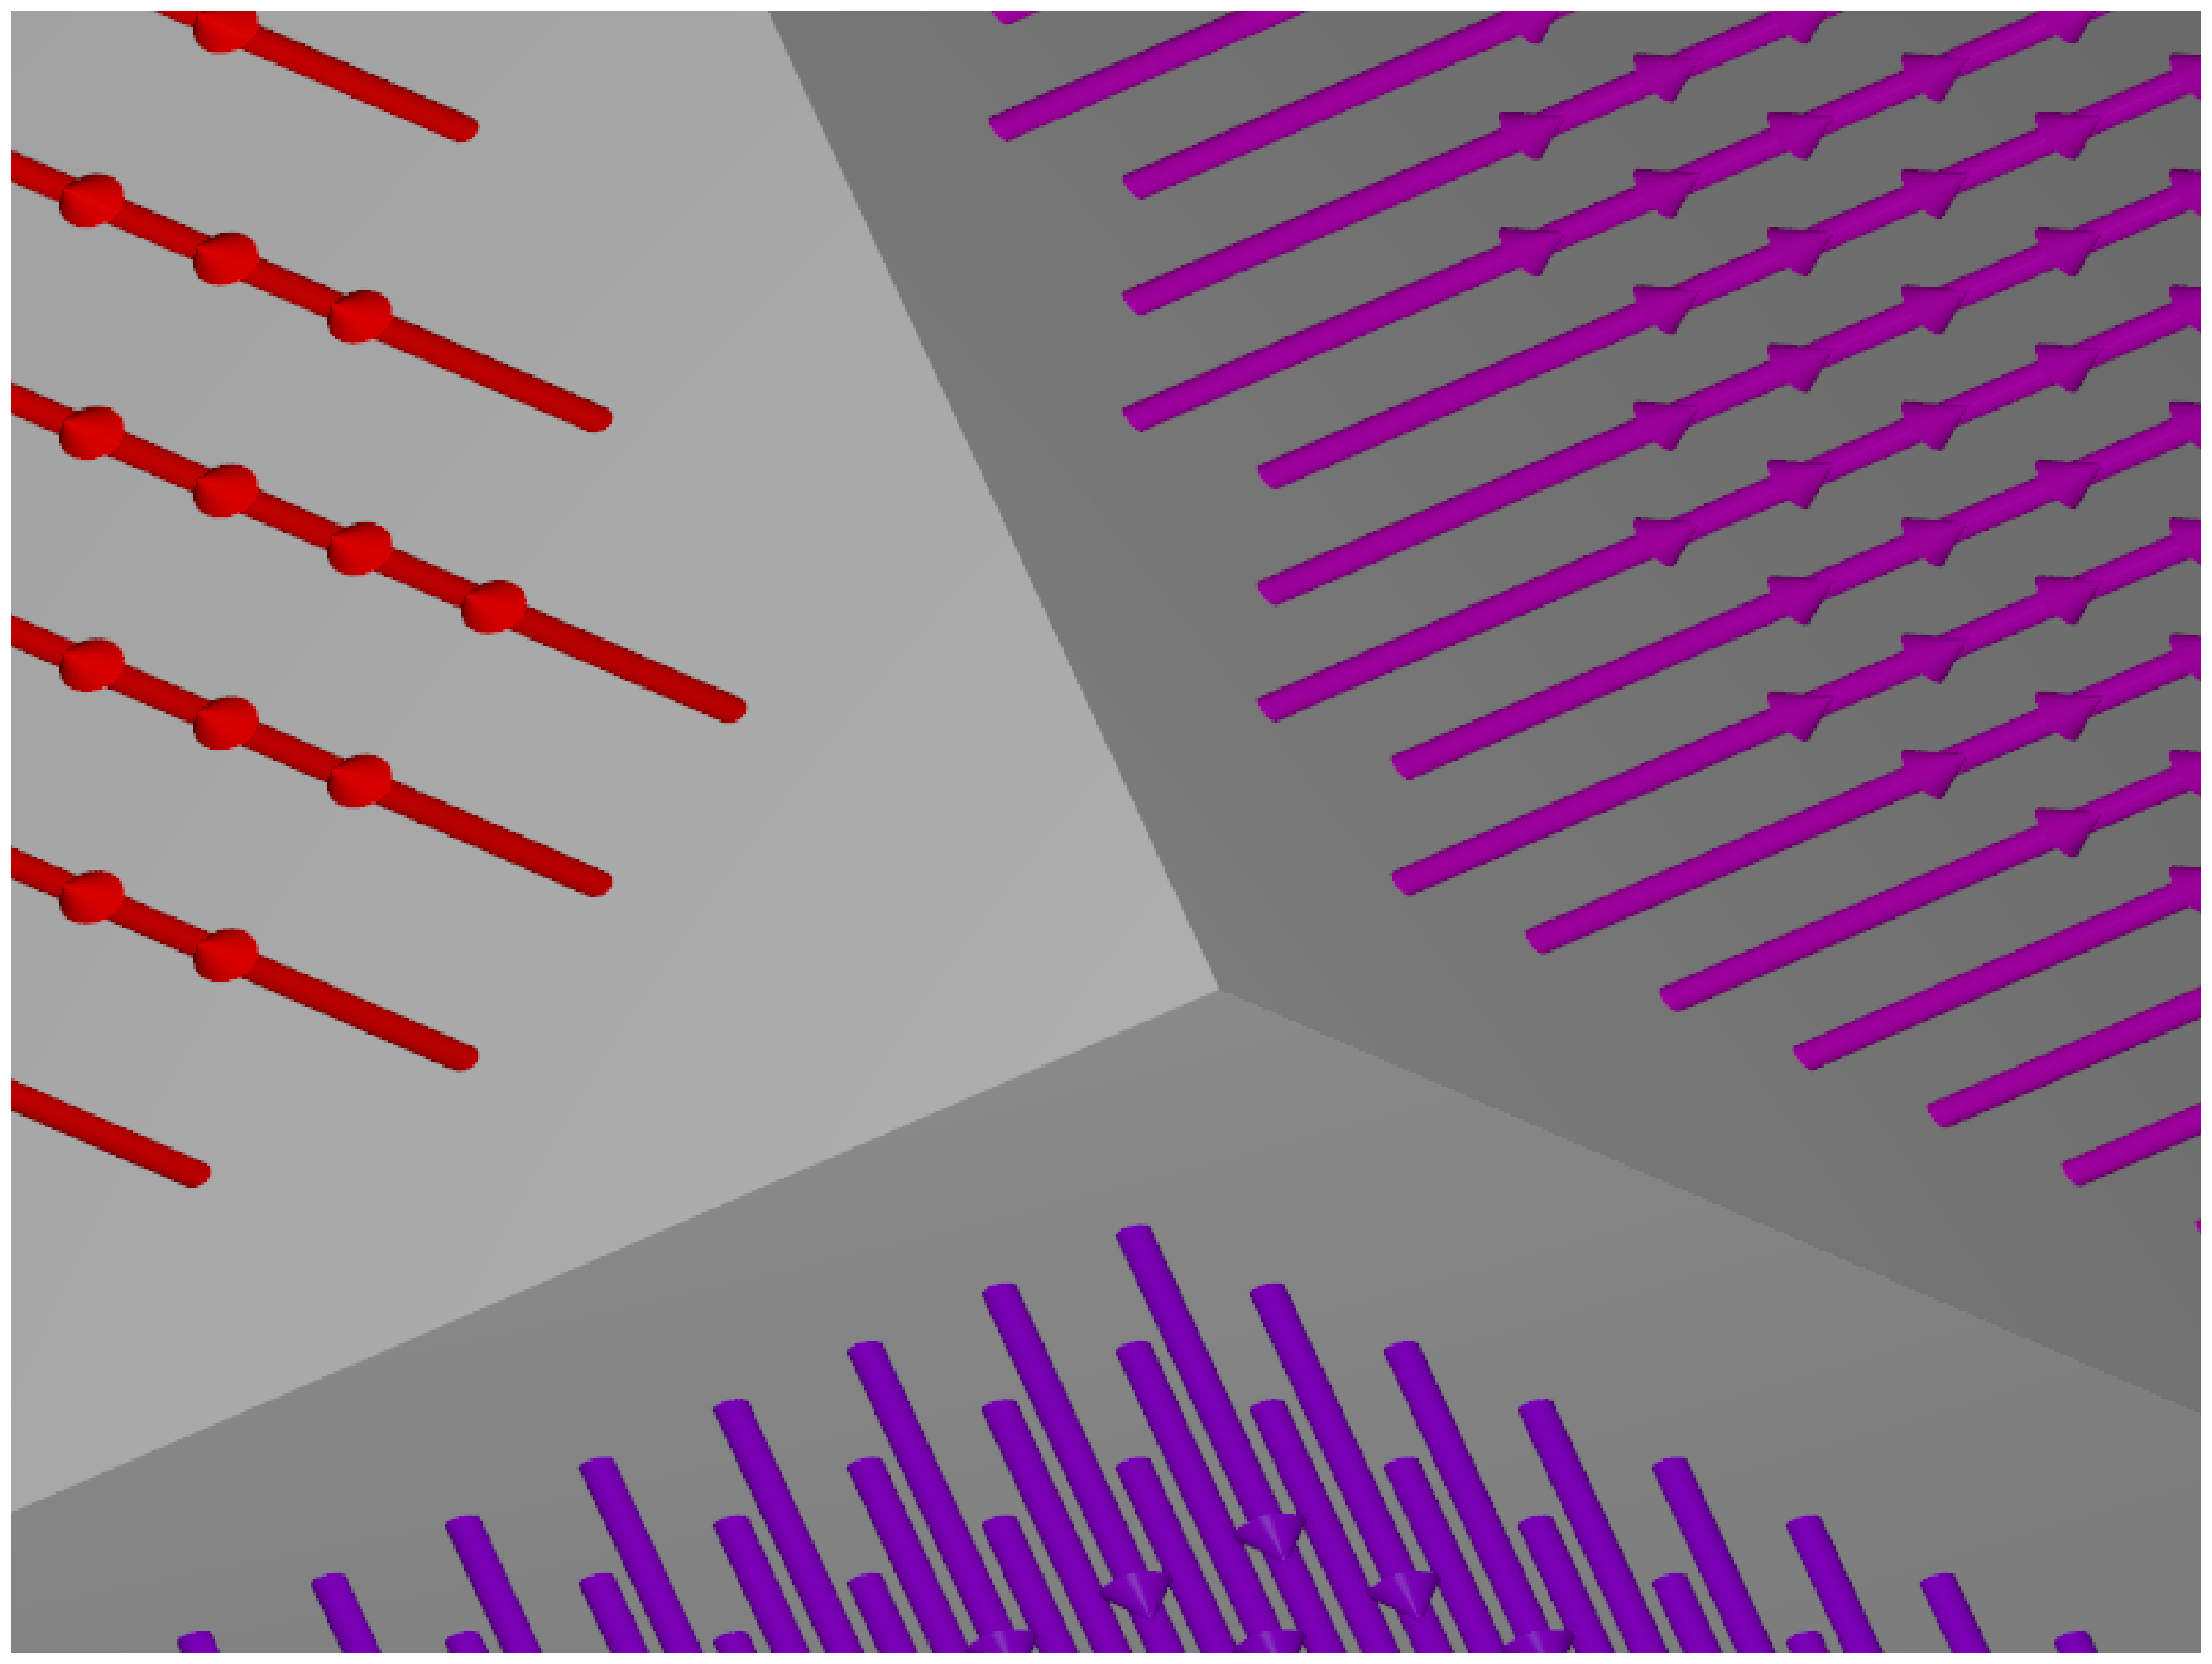
\includegraphics[width=0.25\linewidth]{images/cube.religrad.eps}\label{fig:cube:religrad}}
    \subfloat[]{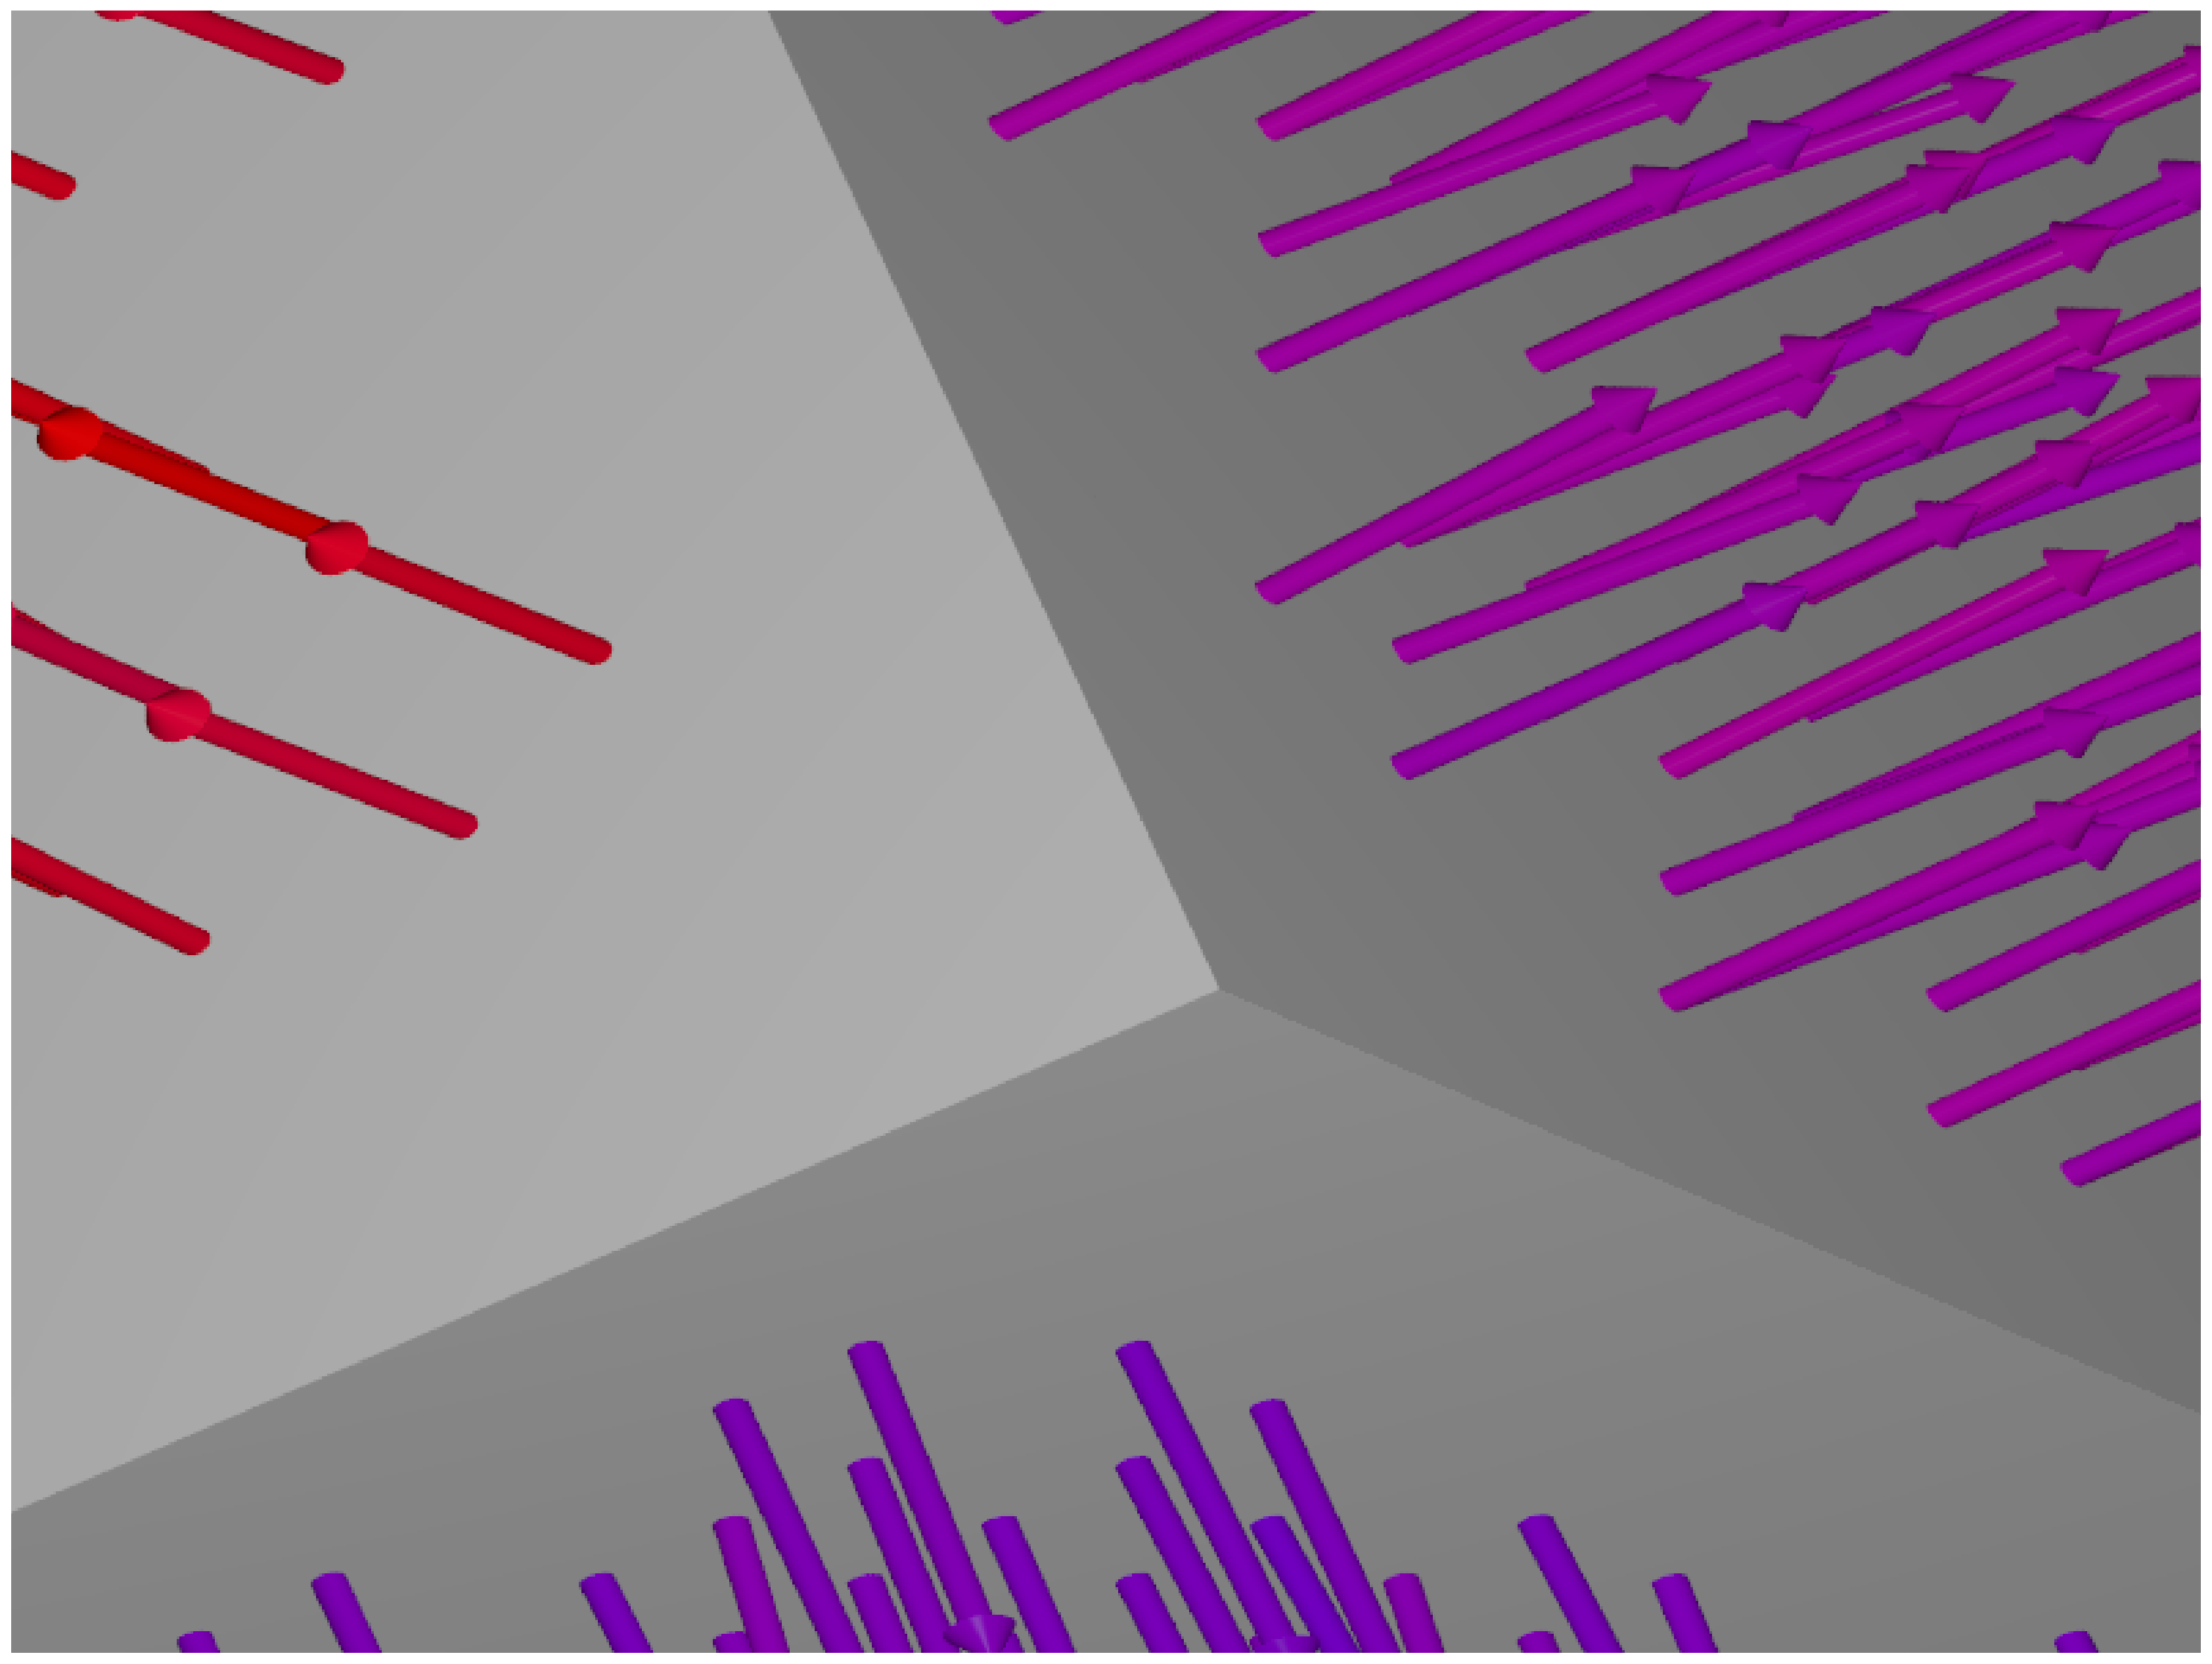
\includegraphics[width=0.25\linewidth]{images/cube.noise.religrad.eps}\label{fig:cube:noise:religrad}}\vspace{-3mm}
    \caption{Effect of uniform noise on \textit{cube} gradients. Uniform 0.1 noise was added to vertex scalars.~\protect\subref{fig:cube:cdiff} central difference gradients on the original \textit{cube}, ~\protect\subref{fig:cube:noise:cdiff}  central difference gradients computed on the noisy cube.
    ~\protect\subref{fig:cube:religrad}  gradients marked correct by \protect\ReliGrad on the original \textit{cube}. ~\protect\subref{fig:cube:noise:religrad} gradients at the vertices marked correct by \protect\ReliGrad on the noisy \textit{cube}. }
    \label{fig:cube:noise}
\end{figure}
Figure~\ref{fig:cube:noise} shows the gradients at corner of the \textit{cube} dataset.
Figure~\subref*{fig:cube:cdiff} shows the central difference gradients. As expected, the gradients across the discontinuity are erroneous.
Fig~\subref*{fig:cube:religrad} shows gradients at grid vertices marked correct by \protect\ReliGrad.
The problems of central difference gradients becomes compounded if the scalar values are noisy. We added 0.1 uniform noise to grid vertex scalars of \emph{cube}. Figure~\subref*{fig:cube:noise:cdiff} shows the central difference  gradients computed from the noisy scalars, Figure~\subref*{fig:cube:noise:religrad} shows the result from \ReliGrad.
\subsection{Quantitative Analysis}
For the synthetic tests cases we know the correct gradients at each grid vertex. Consequently, we can quantitatively compare them with reliable gradients results.
 \begin{table}[h]
     \centering
     \begin{tabular}{|c c c c c c|}
         \hline
         Dataset & CDiff & Algo 1 & Algo 2 & \begin{tabular}[c]{@{}l@{}}Find\\ Reliable\end{tabular} &  \begin{tabular}[c]{@{}l@{}}Reli\\ Grad\end{tabular}\\
         \hline
         Cube  & 48.3 & 0.7& 0.0& 0.0& 0.0\\
         Annulus &  44.03 & 2.79 & 0.02 & 0.02 & 0.02 \\
         Flange & 45.4 & 2.1 & 0.04 & 0.04 & 9.8\\
         TwoCube & 61.86 & 6.1 & 0.0 & 0.0 & 19.8\\
         Cannon & 29.7 & 12.3 & 0.5 & 0.5 & 0.5\\
         Cone & 57.5 & 1.6 & 1.11 & 1.11 & 13.1\\ 
         \hline
       \end{tabular}
       \caption{Maximum Angle difference compared to correct gradients in$^\circ$s. $\alpha$,$\alpha2$ is set to 20$^\circ$. A large number of vertices with high angle difference to the correct gradients, means erroneous gradients are being marked correct. Low angles mean the gradients marked reliable are very close to the correct gradient which is desired outcome.}
       \label{table:gradientDiff}
   \end{table}
Table~\ref{table:gradientDiff} shows the maximum angle difference between the known correct gradients and those computed as reliable gradients at each grid vertex $v$. Intuitively this captures false positives. Large maximum angle would mean poor gradients are being marked as correct.
Algorithm 2 which uses vertices at edge distance 3 for $n_v$ has lower angles than Algorithm 1 for all the test cases thus performing better. Figure~\subref*{fig:annulus:algo1} (Algorithm 1) showed one particular example where gradients near the discontinuity were marked correct compared to (Algorithm 2) figure~\subref*{fig:annulus:algo2}.  Central difference as expected generates erroneous gradients near the edges. For the synthetic datasets, \FindReliable, performs similarly to Algorithm 2.~\ReliGrad which extends the \FindReliable gradients by using Algorithm ~\ref{alg:extend} generates larger maximum angle than \FindReliable.
\begin{table}[h]
    \centering
    \begin{tabular}{|c c c c |}
        \hline
        Dataset  & Algorithm 1 & Algorithm 2 & \ReliGrad\\
        \hline
        Annulus  & 3 & 4 &  2\\
        Cube & 3 & 4 & 3\\ 
        Flange & 4 & 6 & 4\\
        Cannon & 2& 4& 2\\
        Cone   & 3& 4& 2\\
        TwoCube & 4& 5& 3\\ \hline
    \end{tabular}
    \caption{Maximum of minimum L1 distance to grid vertices with exact gradient.}
    \label{table:gradientinfo}
\end{table}

Next we look at the maximum of the minimum L1 distances from each vertex $v$ without a reliable gradient, to a grid vertex $v_2$ with a reliable gradient (dist2religrad). Table~\ref{table:gradientinfo} shows the results. This test intuitively captures false negatives. Large dist2religrad, would mean more vertices with reliable gradients are being marked unreliable. It is desirable for algorithms which use the reliable gradients results, that the L1 distance of  an unreliable vertex $v$ to it's closest reliable vertex $v_2$ be as small as possible. For \textit{Annulus} there is a grid vertex at maximum L1 edge distance of 4 from each $v$ when using Algorithm~\ref{alg:phi2}. For \textit{Cube} there is a vertex with correct gradient within L1 edge distance 4 from each $v$ when using Algorithm~\ref{alg:phi2}. When we extend the reliable gradients and use \ReliGrad,  the maximum L1 distance decreases to 2 and 3 respectively. Experimentally we found and as shown in  figure~\subref*{fig:cube:religrad}, the dist2grad for \textit{Cube} is maximum near the corners. 
\textbf{Noise}:
To test the effect of noise on \ReliGrad, uniform noise was added to the datasets. Table~\ref{table:noise} shows the results. With 0.1 uniform noise \ReliGrad performs well. The dist2grad of 5 for the \textit{Cube} dataset is near the corner (figure~\subref*{fig:cube:noise:religrad}). With a high uniform noise of 0.2, and $\alpha_{2}$ in \ReliGrad set to 30$^{\circ}$s we perform reasonably well. 
\tiny
\begin{table}[htb]
    \begin{tabular}{|l|l|l|l|l|}
        \hline
        dataset & noise & \begin{tabular}[c]{@{}l@{}}$\alpha_{2}$\\ in $^{\circ}$\end{tabular} & \begin{tabular}[c]{@{}l@{}}Max\\ AngleDiff in $^{\circ}$\end{tabular} & \begin{tabular}[c]{@{}l@{}}Dist\\ 2Grad\end{tabular} \\ \hline
        cube    & 0.1   & 20                                                                   & 7.5                                                                  & 5         \\ \hline
        annulus & 0.1   & 20                                                                   & 8.1                                                                  & 3         \\ \hline
        cone    & 0.1   & 20                                                                   & 12.7                                                                 & 3         \\ \hline
        cube    & 0.2   & 30                                                                   & 12.8                                                                 & 7         \\ \hline
        annulus & 0.2   & 30                                                                   & 14.1                                                                 & 5         \\ \hline
        cone    & 0.2   & 30                                                                   & 19                                                                   & 6         \\ \hline
    \end{tabular}
    	\caption{Results after adding 0.1 and 0.2 uniform noise to the datasets using \protect\ReliGrad. To handle 0.2 noise we set $\alpha_{2}$ to be 30$^{\circ}$s. MaxAngleDiff, measures the maximum angle difference between known correct gradients and those marked correct by \protect\ReliGrad. Dist2Grad measures the maximum of the l1 distance of the unreliable vertices to vertices marked correct by \protect\ReliGrad.}
        \label{table:noise}
\end{table}
\normalsize
\subsection{Industrial CT data} 
\begin{table}[hb]
	\centering
	\begin{tabular}{|c c c |} 
		\hline
		Name & Axis Size & Spacing  \\ [0.5ex] 
		\hline
        CMM & 500 500 196 & 0.2 0.2 0.31\\
		Engine cylinder & 201 130 63 & 0.27 0.27 0.68 \\
        Intake &  150 220 201 & 0.27 0.27 0.68 \\
        Socket & 411 431 61 & 1 1 1 \\
		\hline
	\end{tabular}
	\caption{CT dataset information}
	\label{table:ictDataInfo}
\end{table}
\begin{figure}[htb]
    \centering
    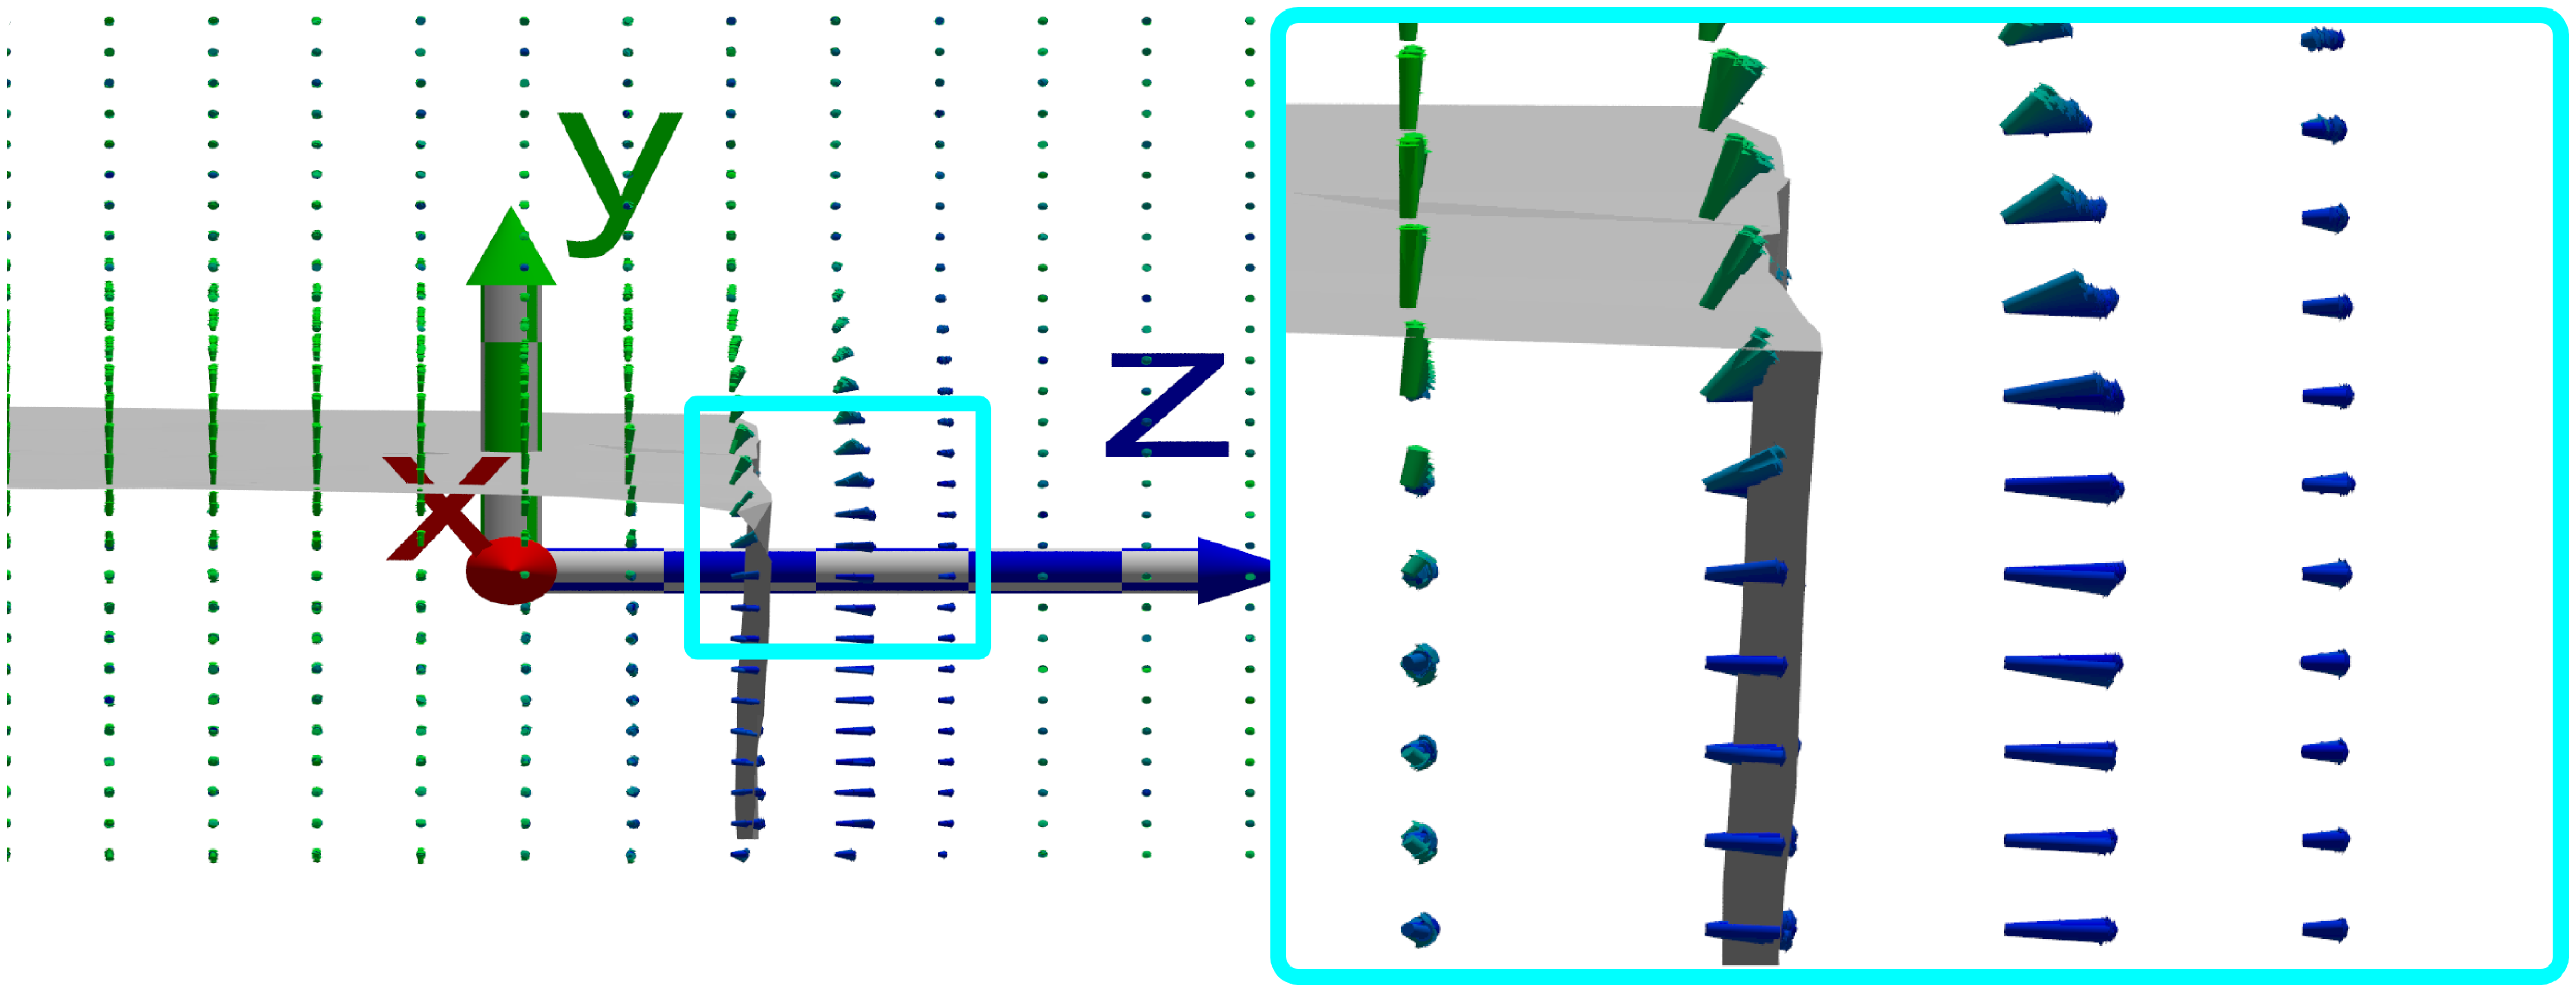
\includegraphics[width=\linewidth]{images/cdiff.all.new.eps}
    \caption{All the central difference gradients on  grid vertices of a small portion of the \textit{engine cylinder} dataset
	(Figure~\ref{fig:grad-1} shows the same regions, 
	but only the gradients at vertices intersected by isosurface).
	The gradient magnitudes are proportional to length of the vectors.
	On the right we see a magnified section of the cyan rectangle.
    The grid magnitudes drop off quickly, and the gradient directions become meaningless especially along the Z-axis. 
    }
    \label{fig:setA.crop1.cdiff}
\end{figure}
\begin{figure}
    \centering
    \subfloat[]{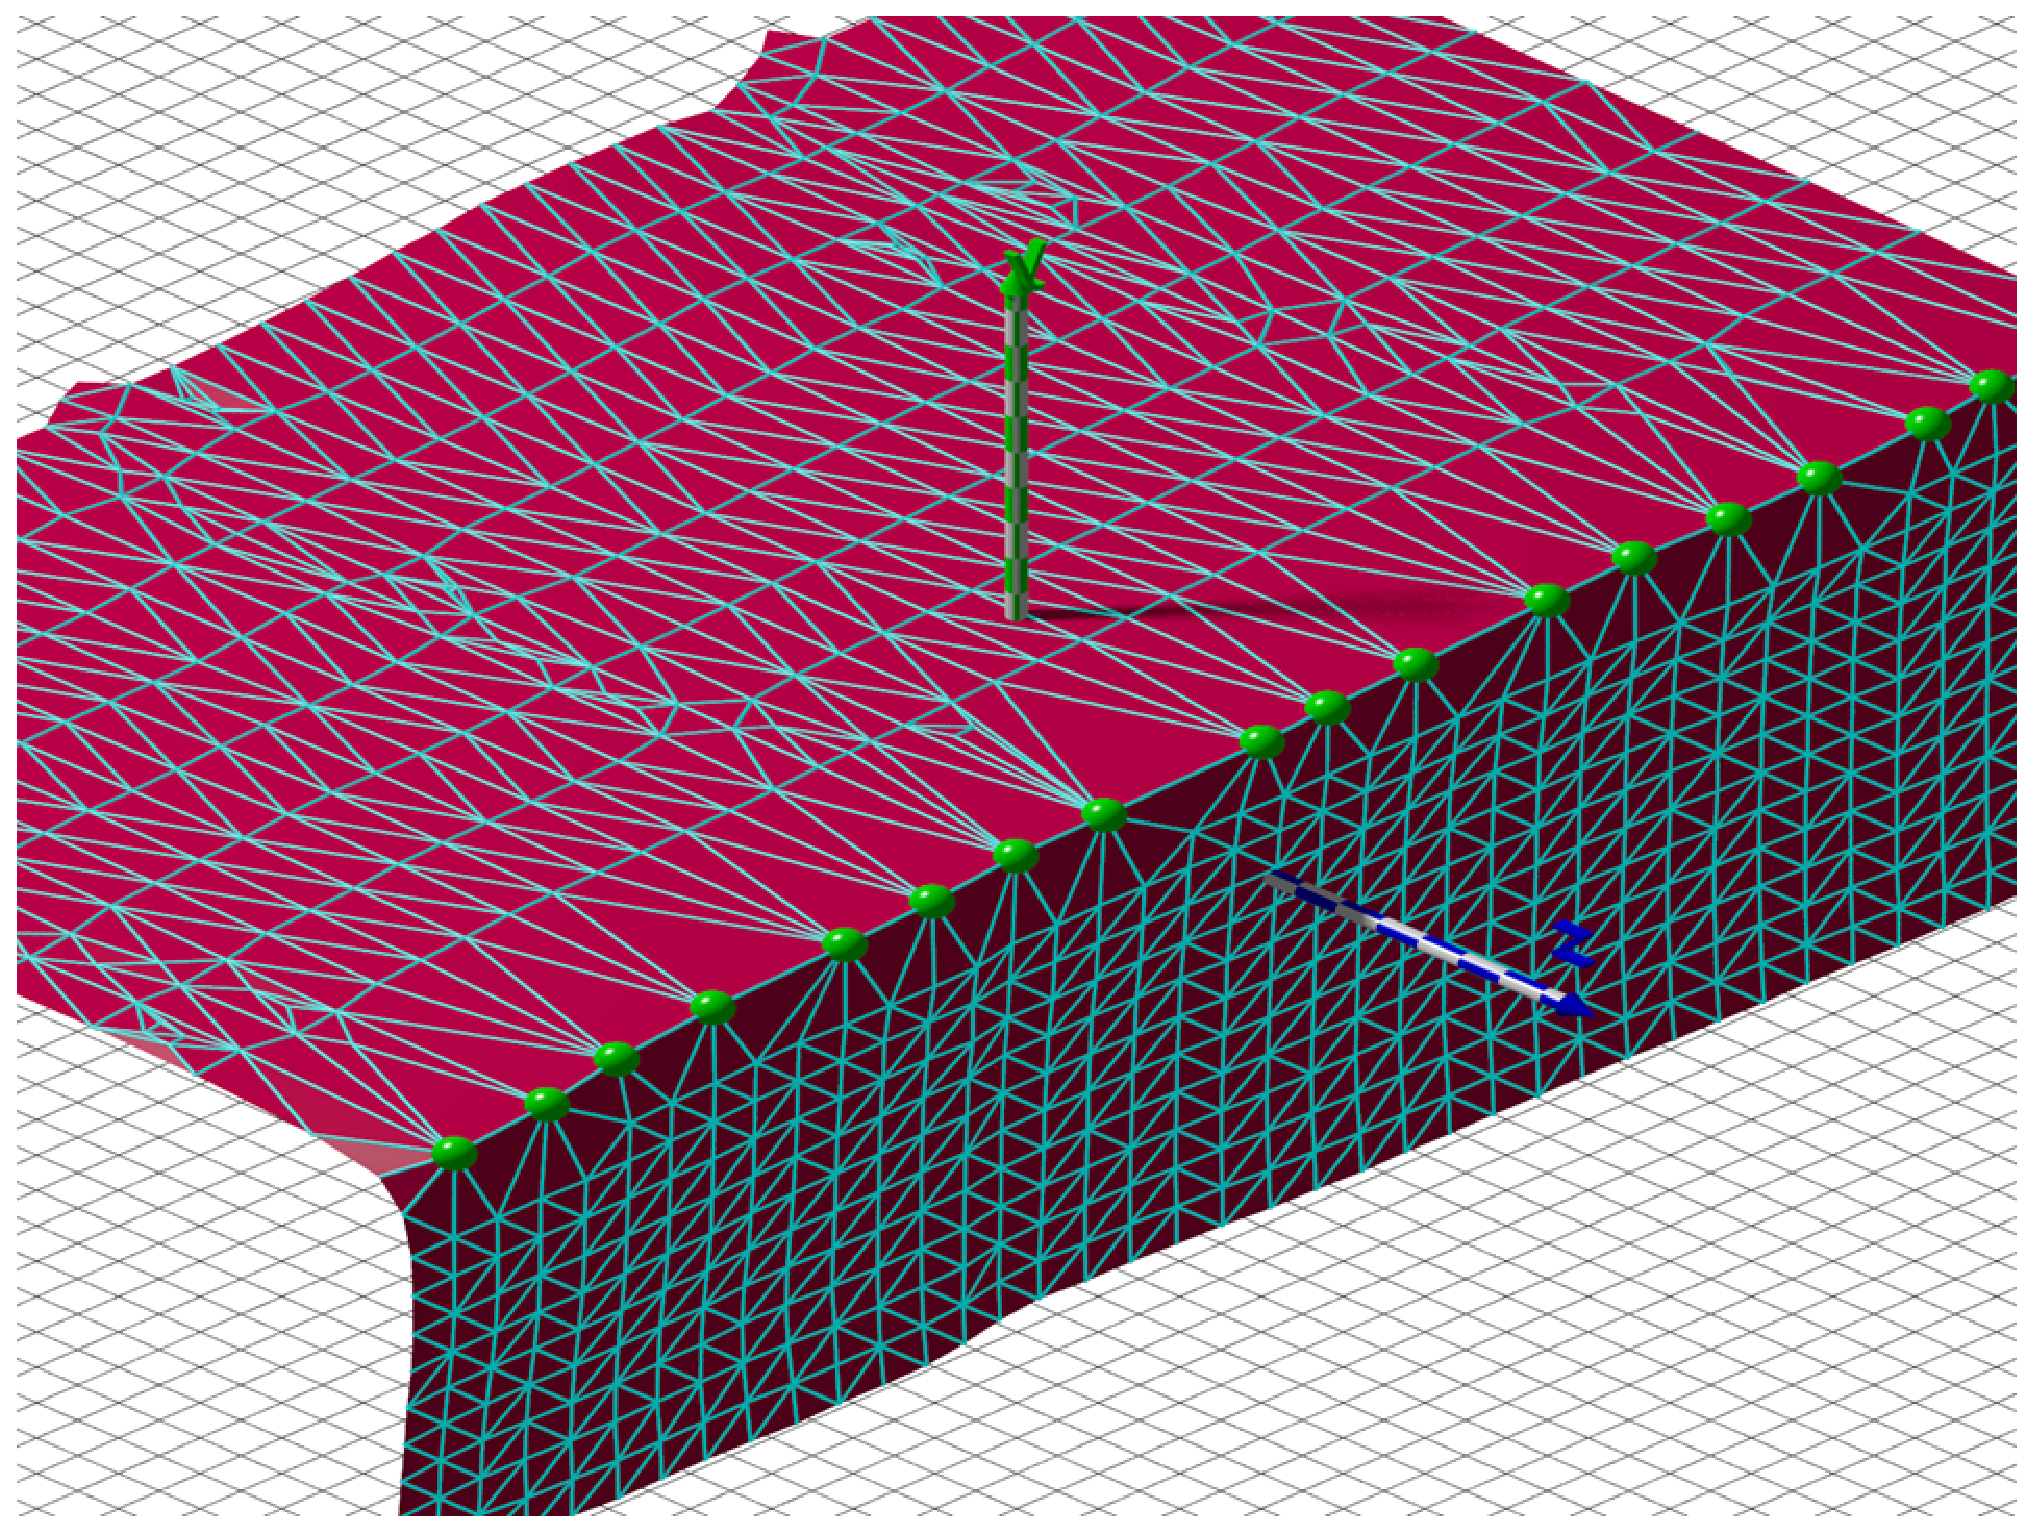
\includegraphics[width=0.33\linewidth]{images/setA.crop2.mesh.eps}\label{fig:setA.crop1.mesh.1}}
    \subfloat[]{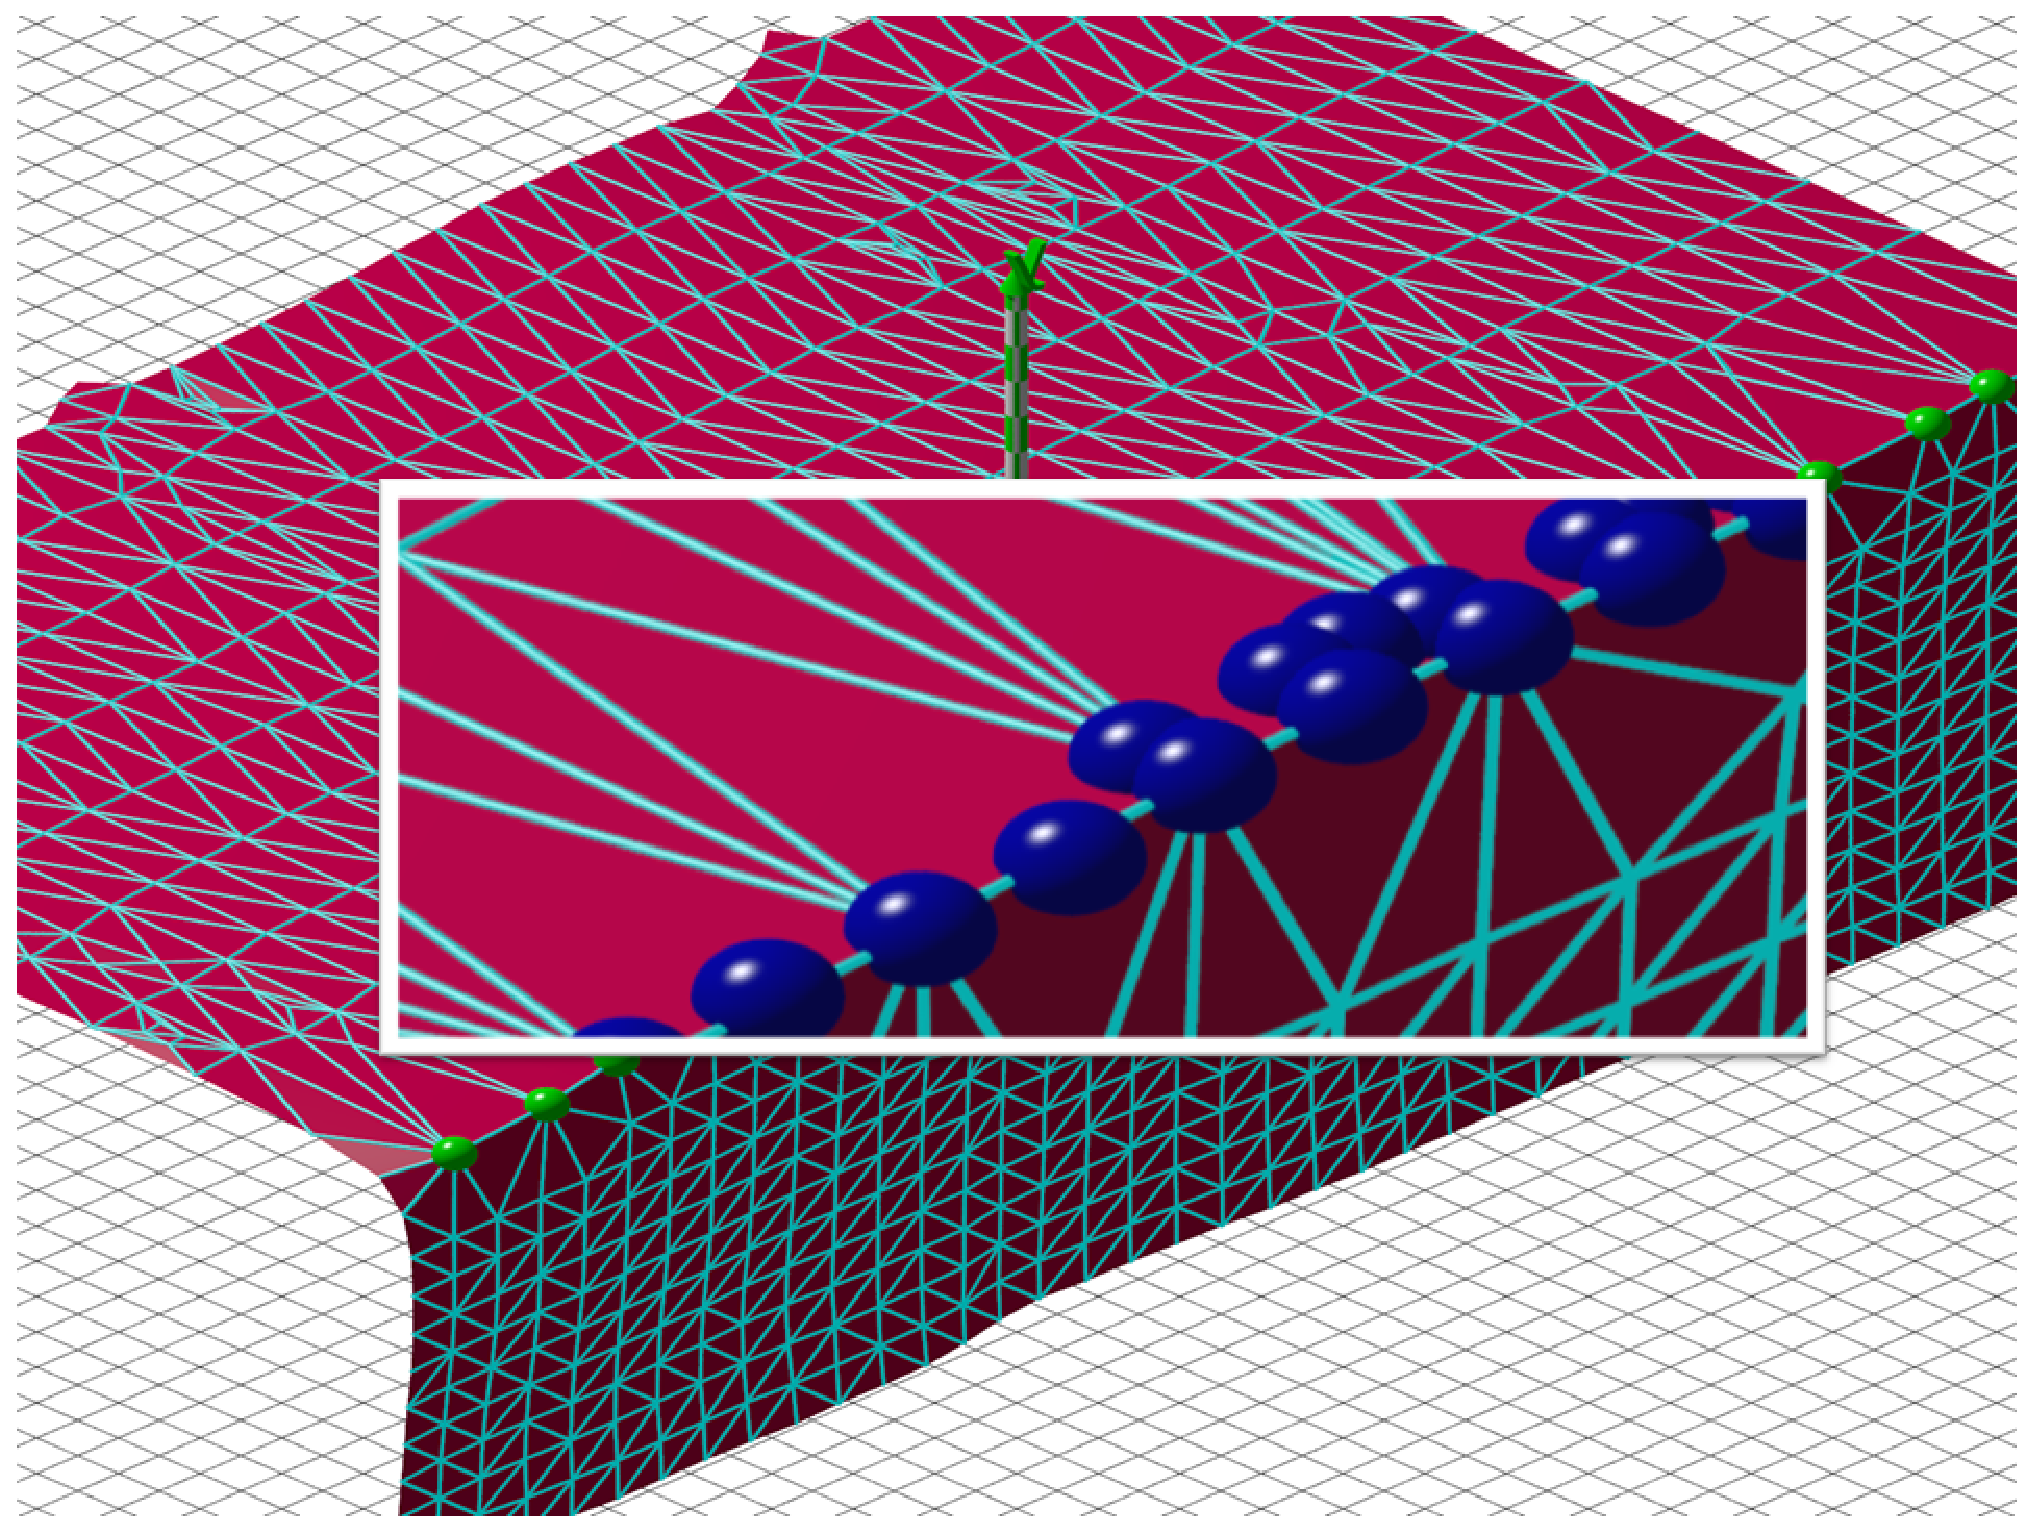
\includegraphics[width=0.33\linewidth]{images/mesh.edges.all.eps}\label{fig:setA.crop1.mesh.2}}
    \subfloat[]{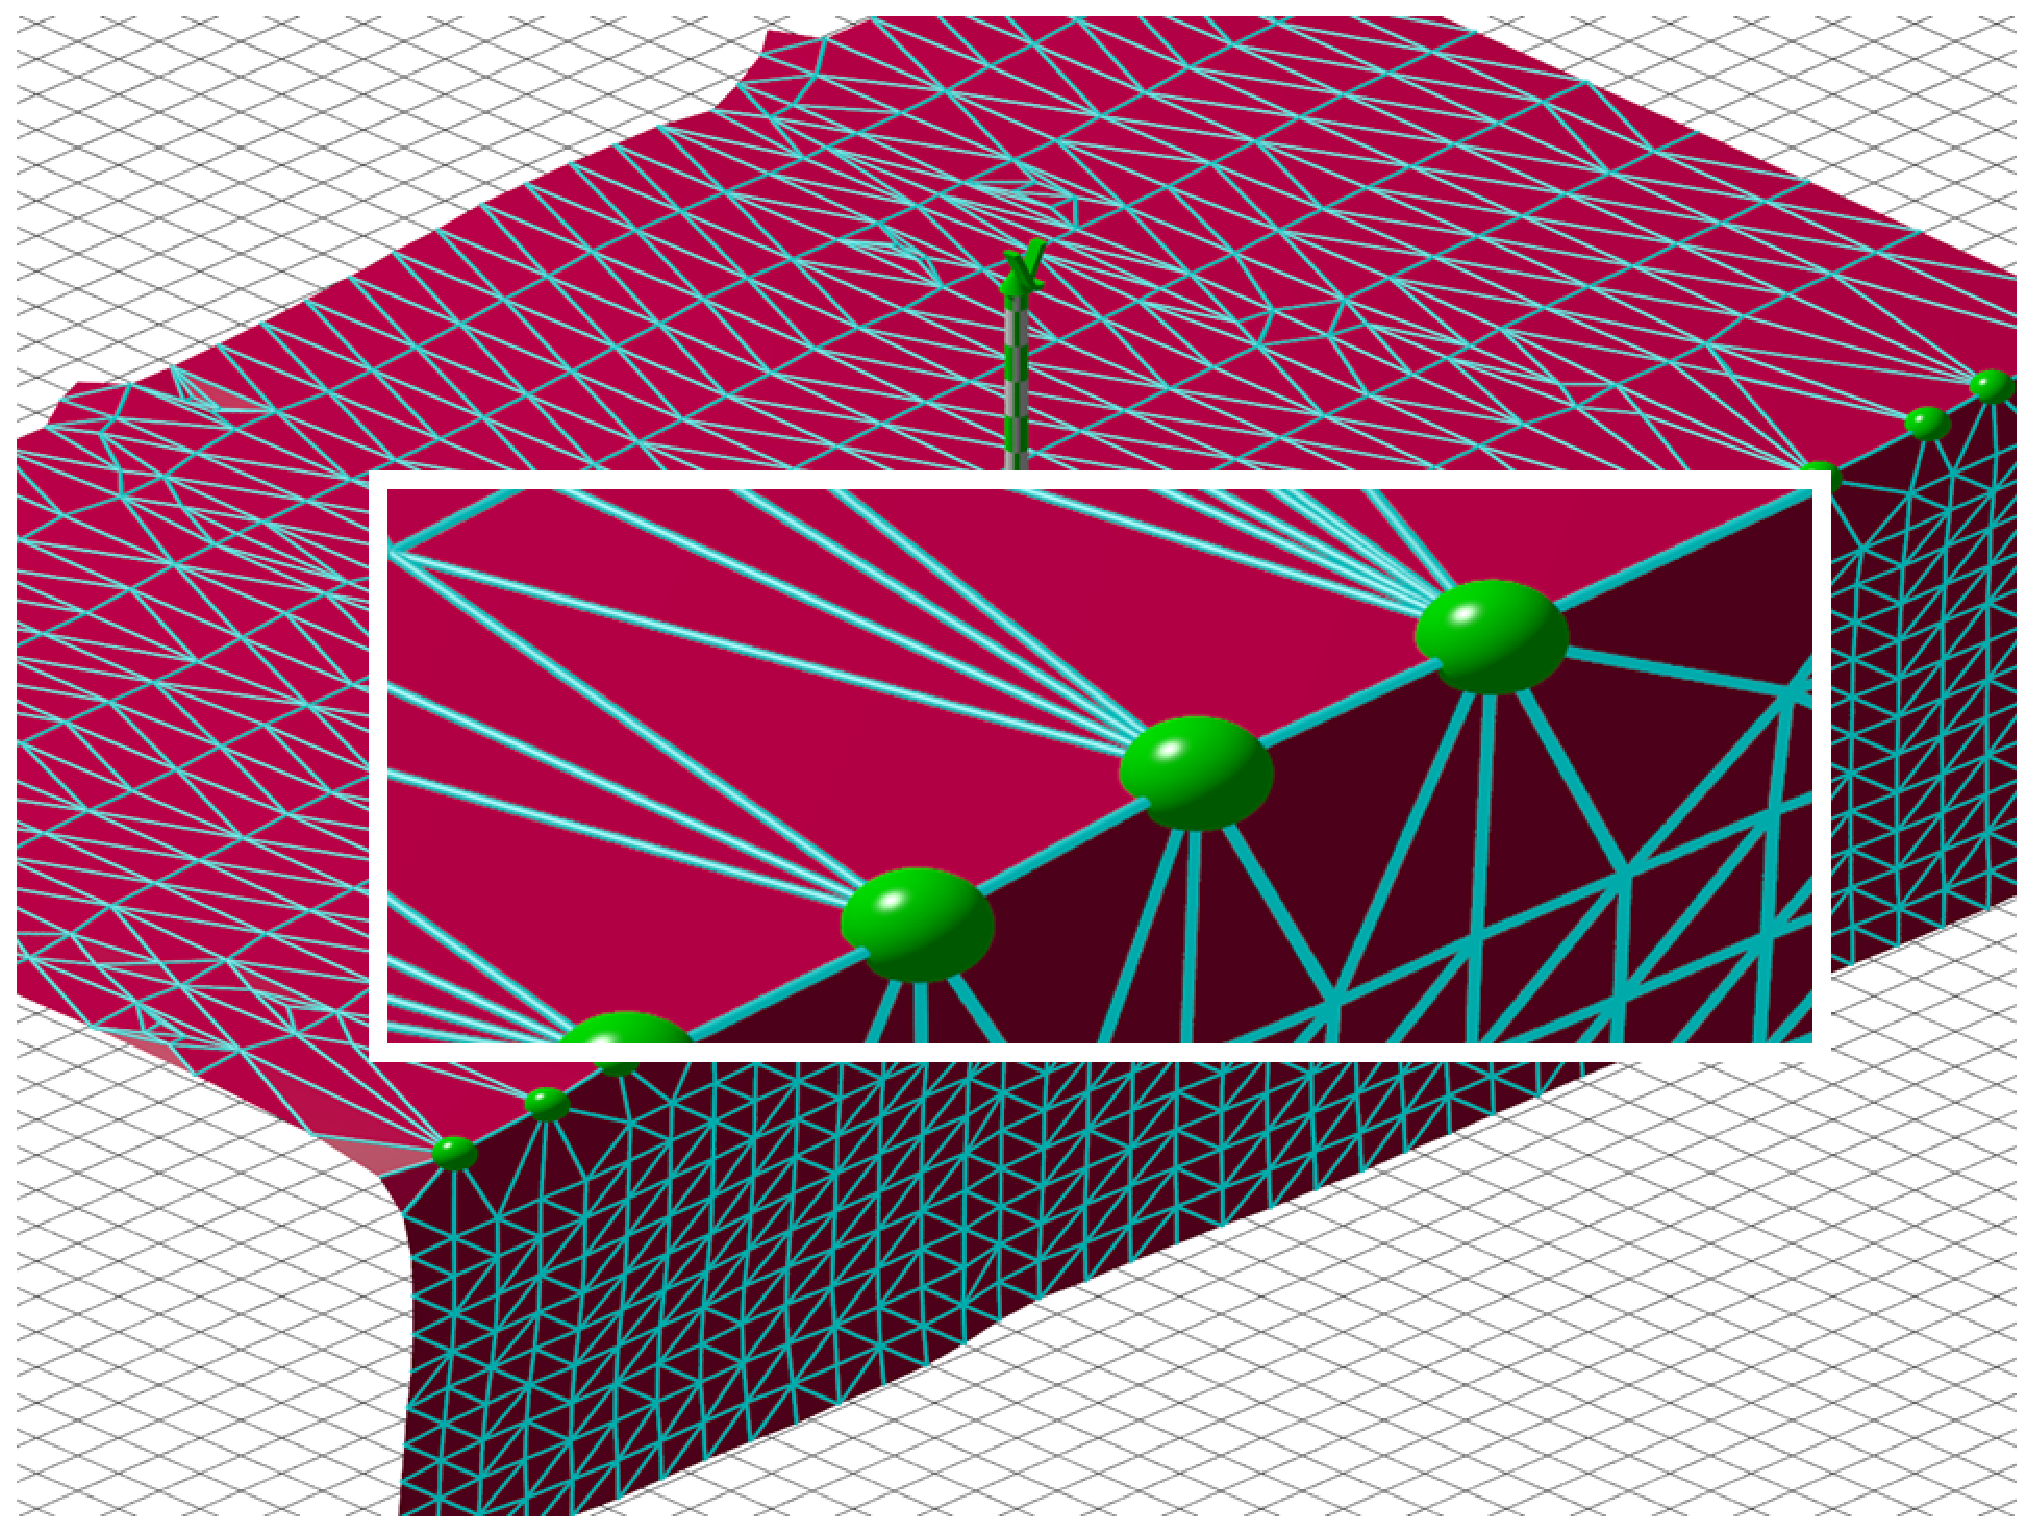
\includegraphics[width=0.33\linewidth]{images/mesh.edges.eps}\label{fig:setA.crop1.mesh.3}}
   \caption{~\protect\subref*{fig:setA.crop1.mesh.1}(Part of cylinder dataset (Figure~\ref{fig:setA.crop1}). The features vertices are generated using \protect\ReliGrad gradients (figure~\ref{fig:setA.crop1.religrad})}
   \label{fig:setA.crop1.mesh}
\end{figure}
\begin{figure}
    \centering
     \subfloat[Algorithm 1 gradients]
     {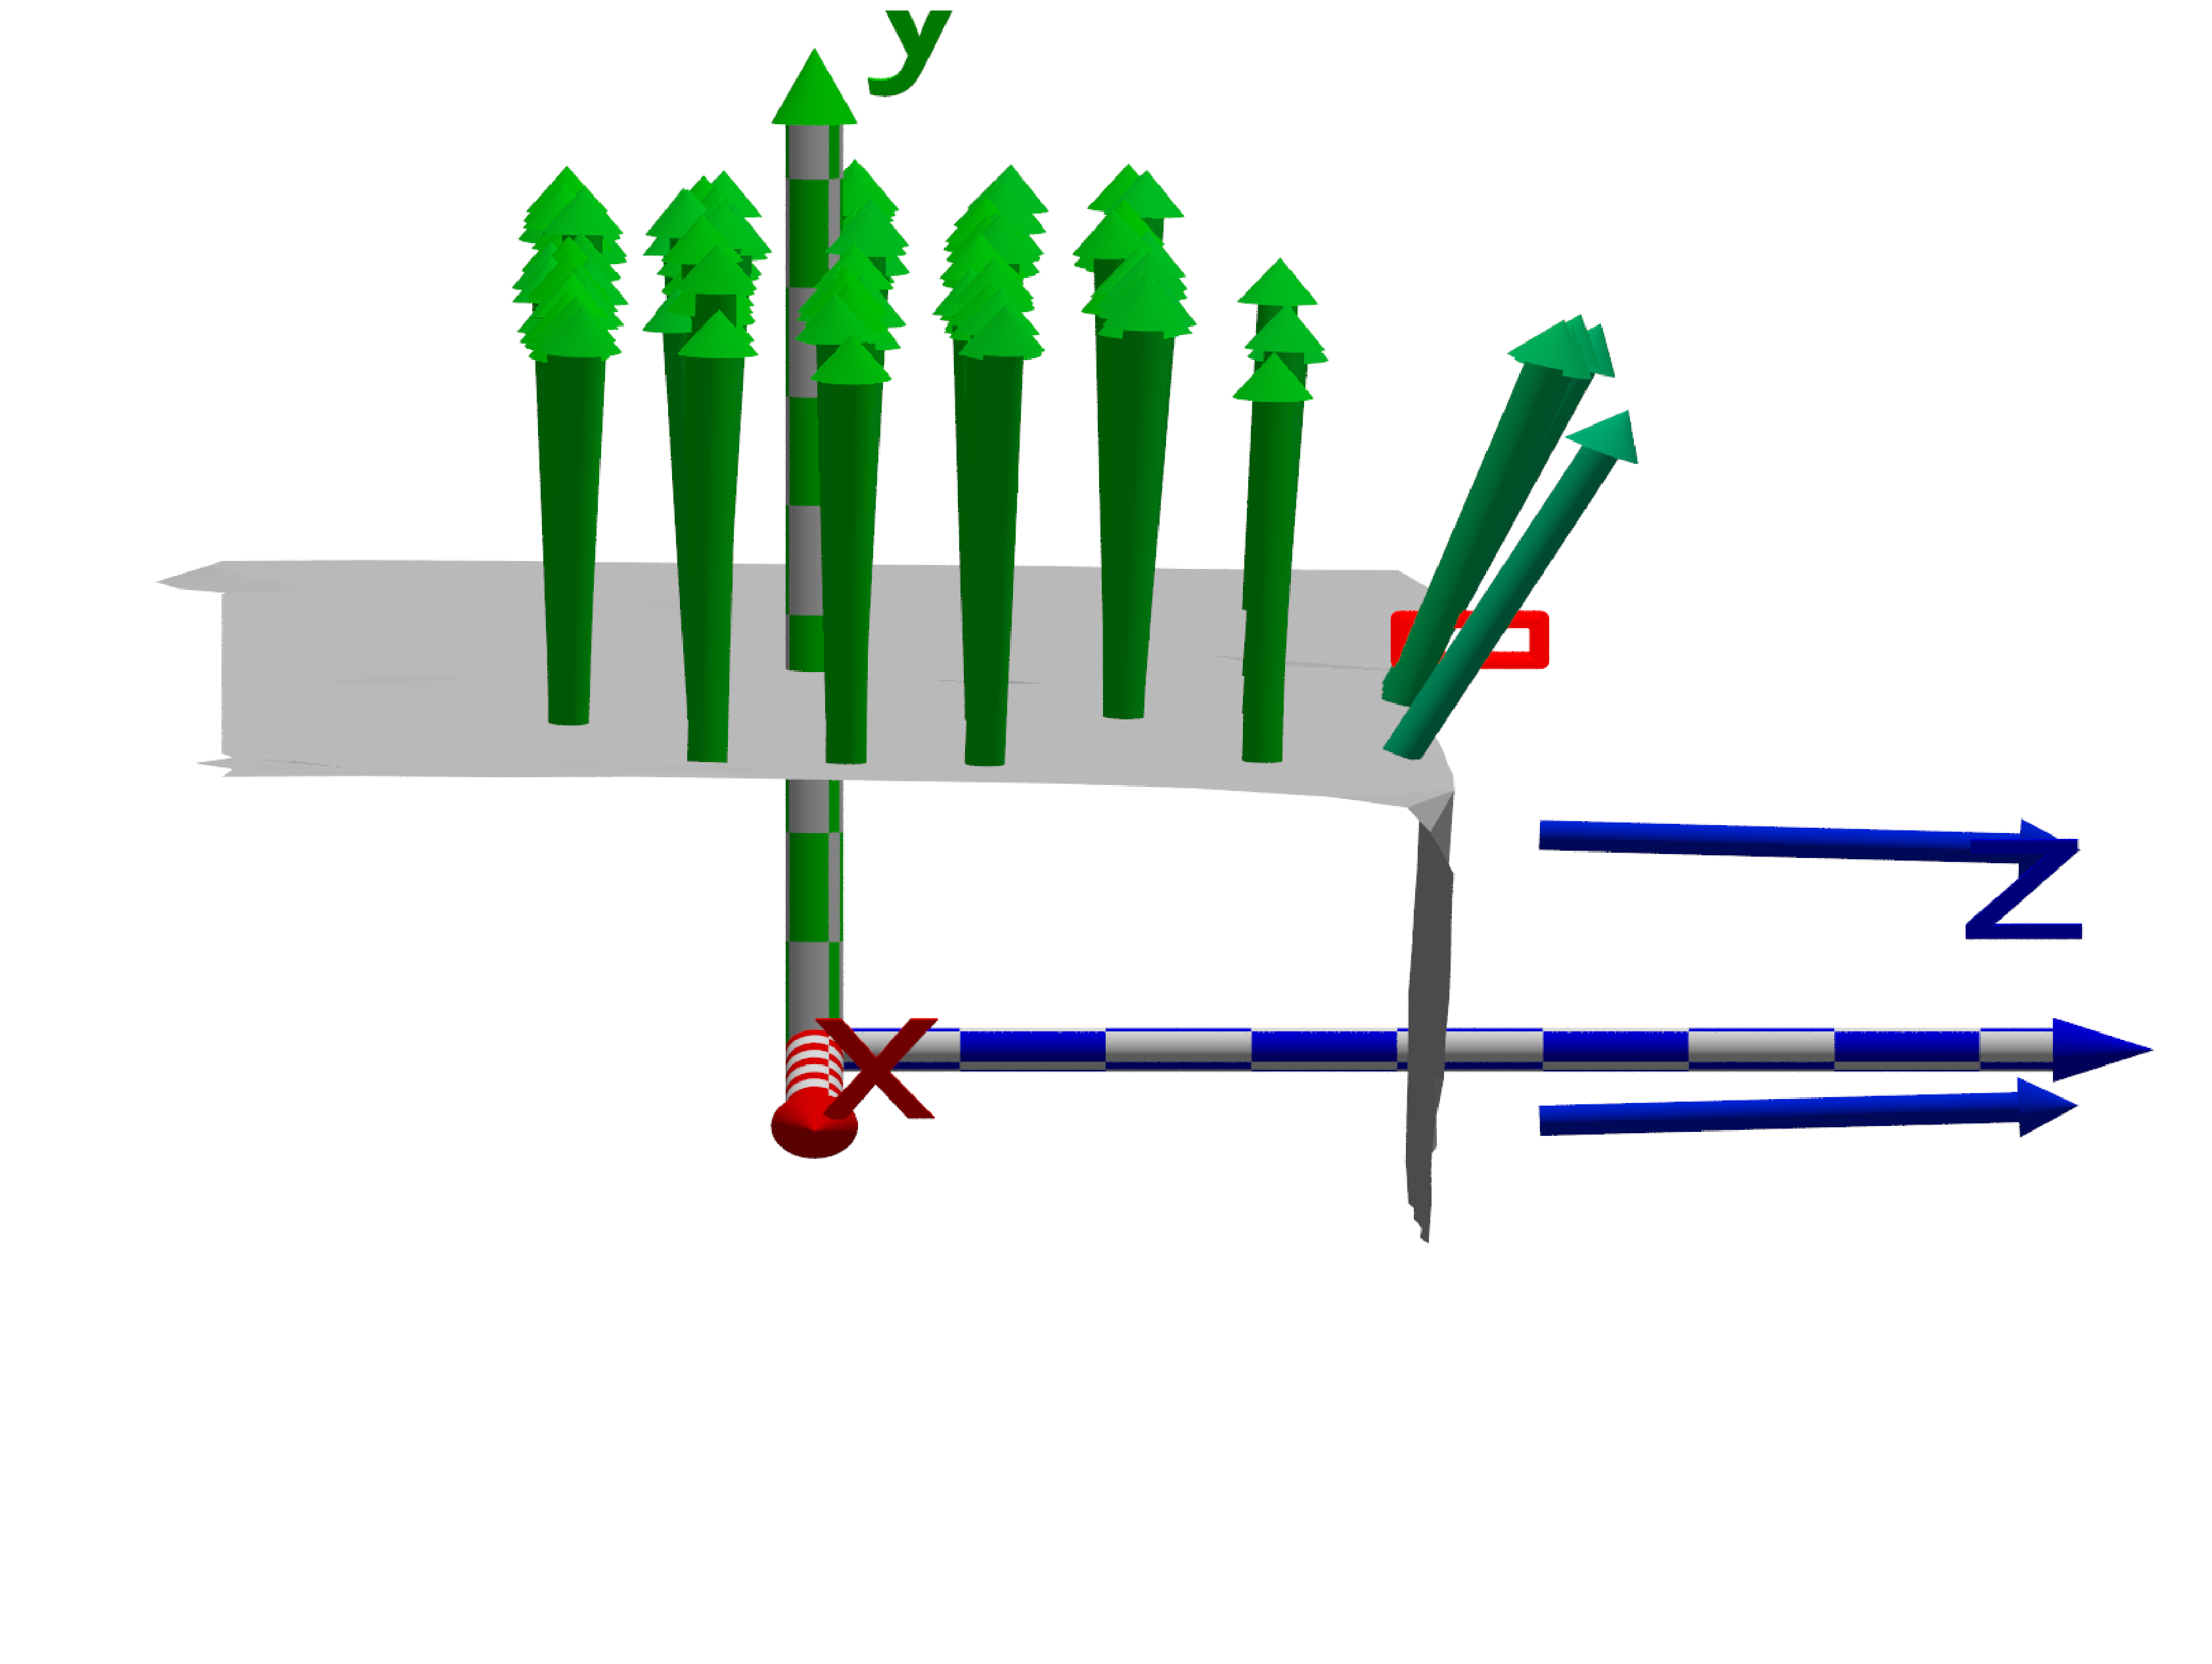
\includegraphics[width=0.25\linewidth ]{images/setA.crop2.algo1.new.eps}\label{fig:setA.crop1.algo1}}
     \subfloat[Algorithm 2 gradients]{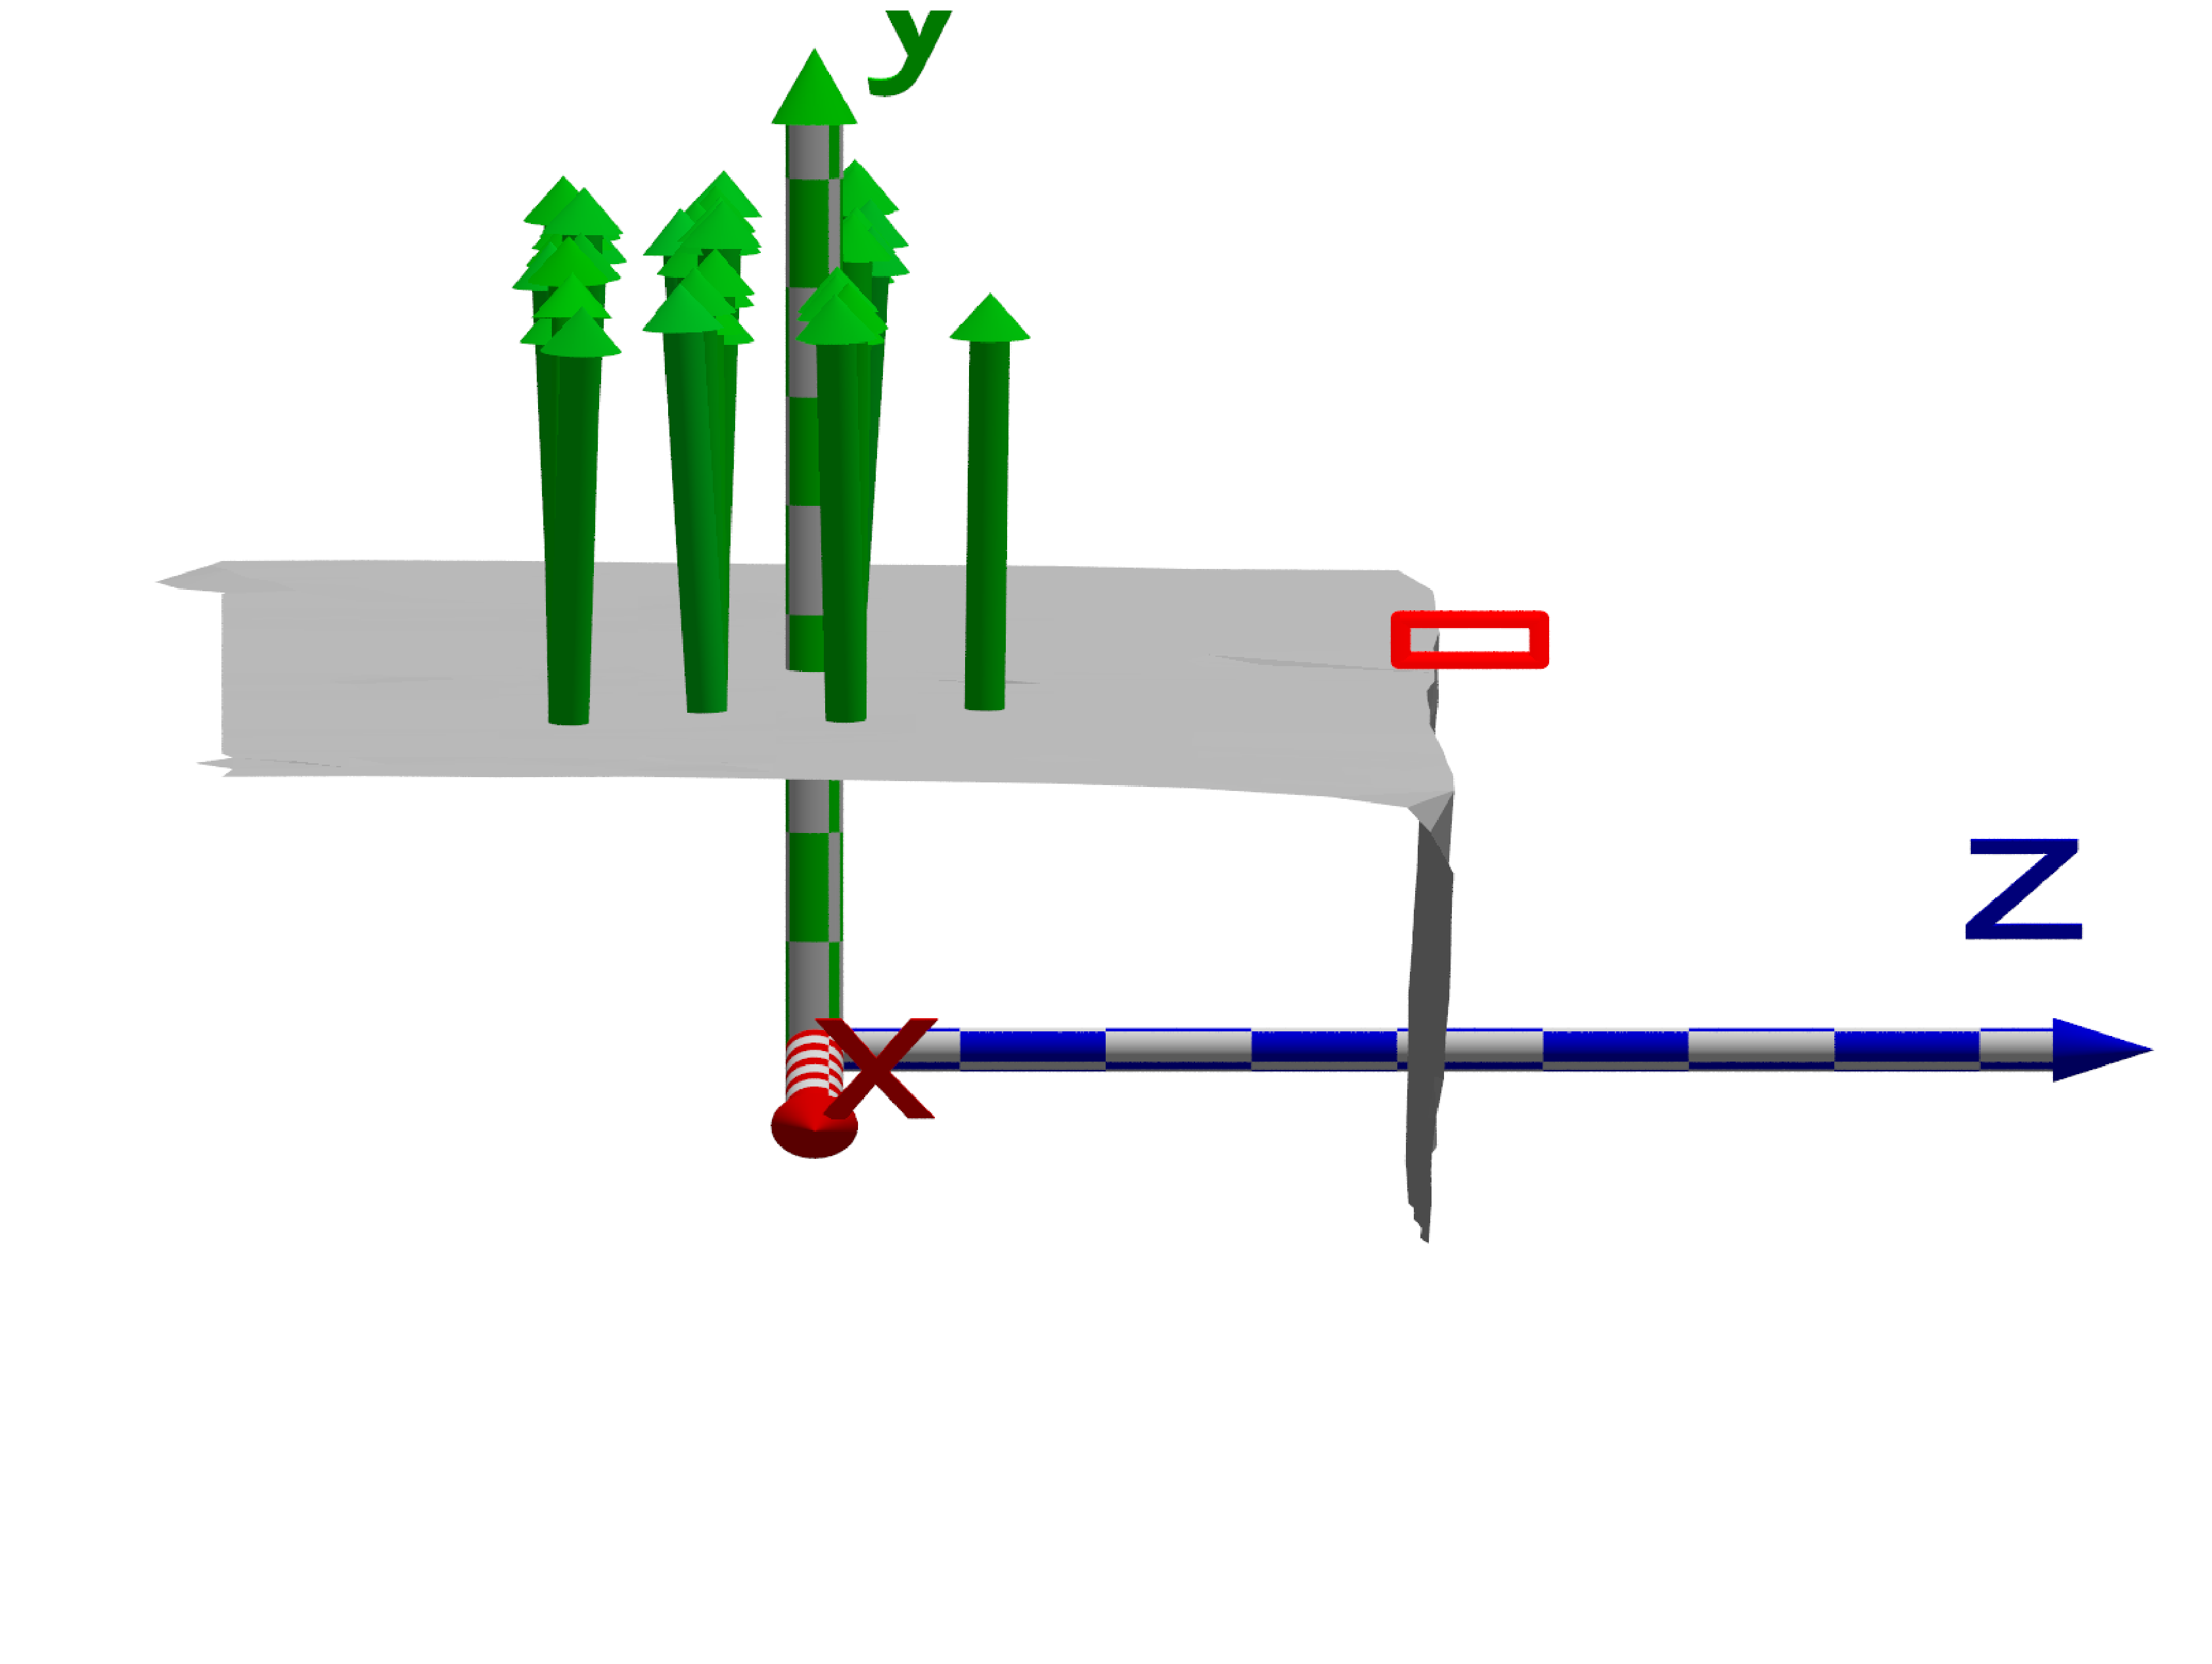
\includegraphics[width=0.25\linewidth]{images/setA.crop2.algo2.new.eps}\label{fig:setA.crop1.algo2}}
     \subfloat[FindReliable gradients]{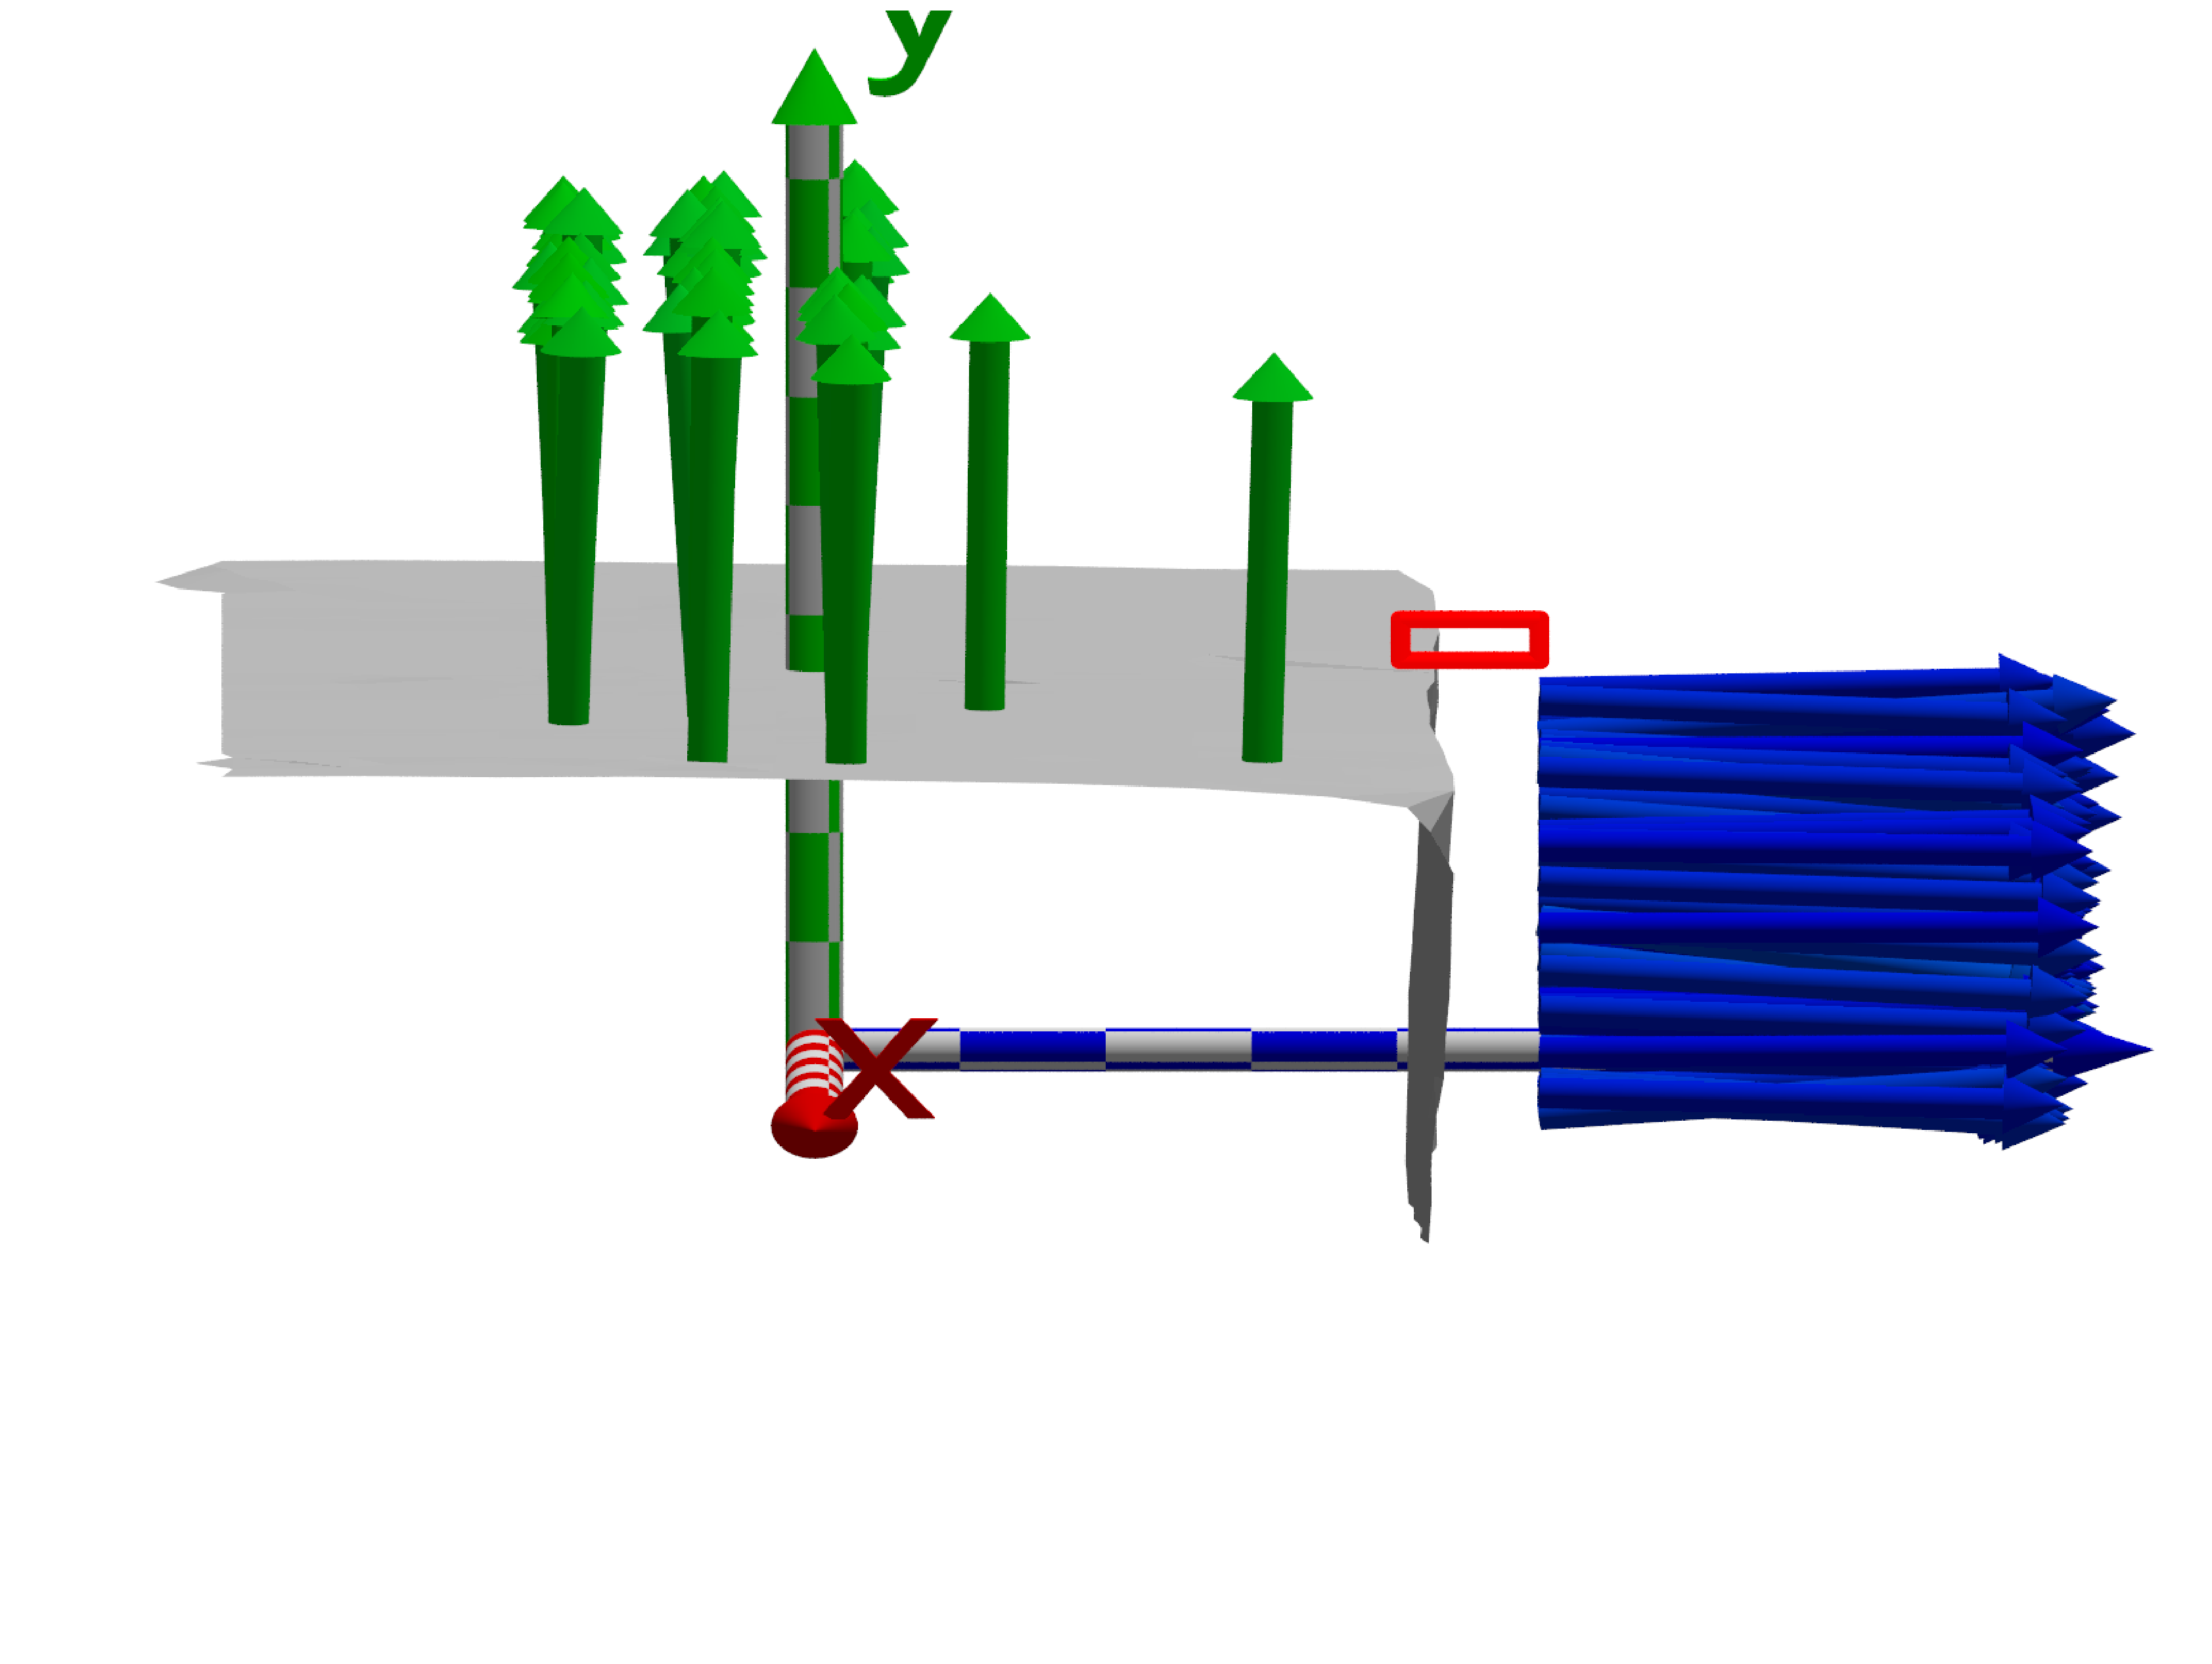
\includegraphics[width=0.25\linewidth]
             {images/setA.crop2.findReliable.new.eps}\label{fig:setA.crop1.findReliable}}
     \subfloat[ReliGrad gradients]{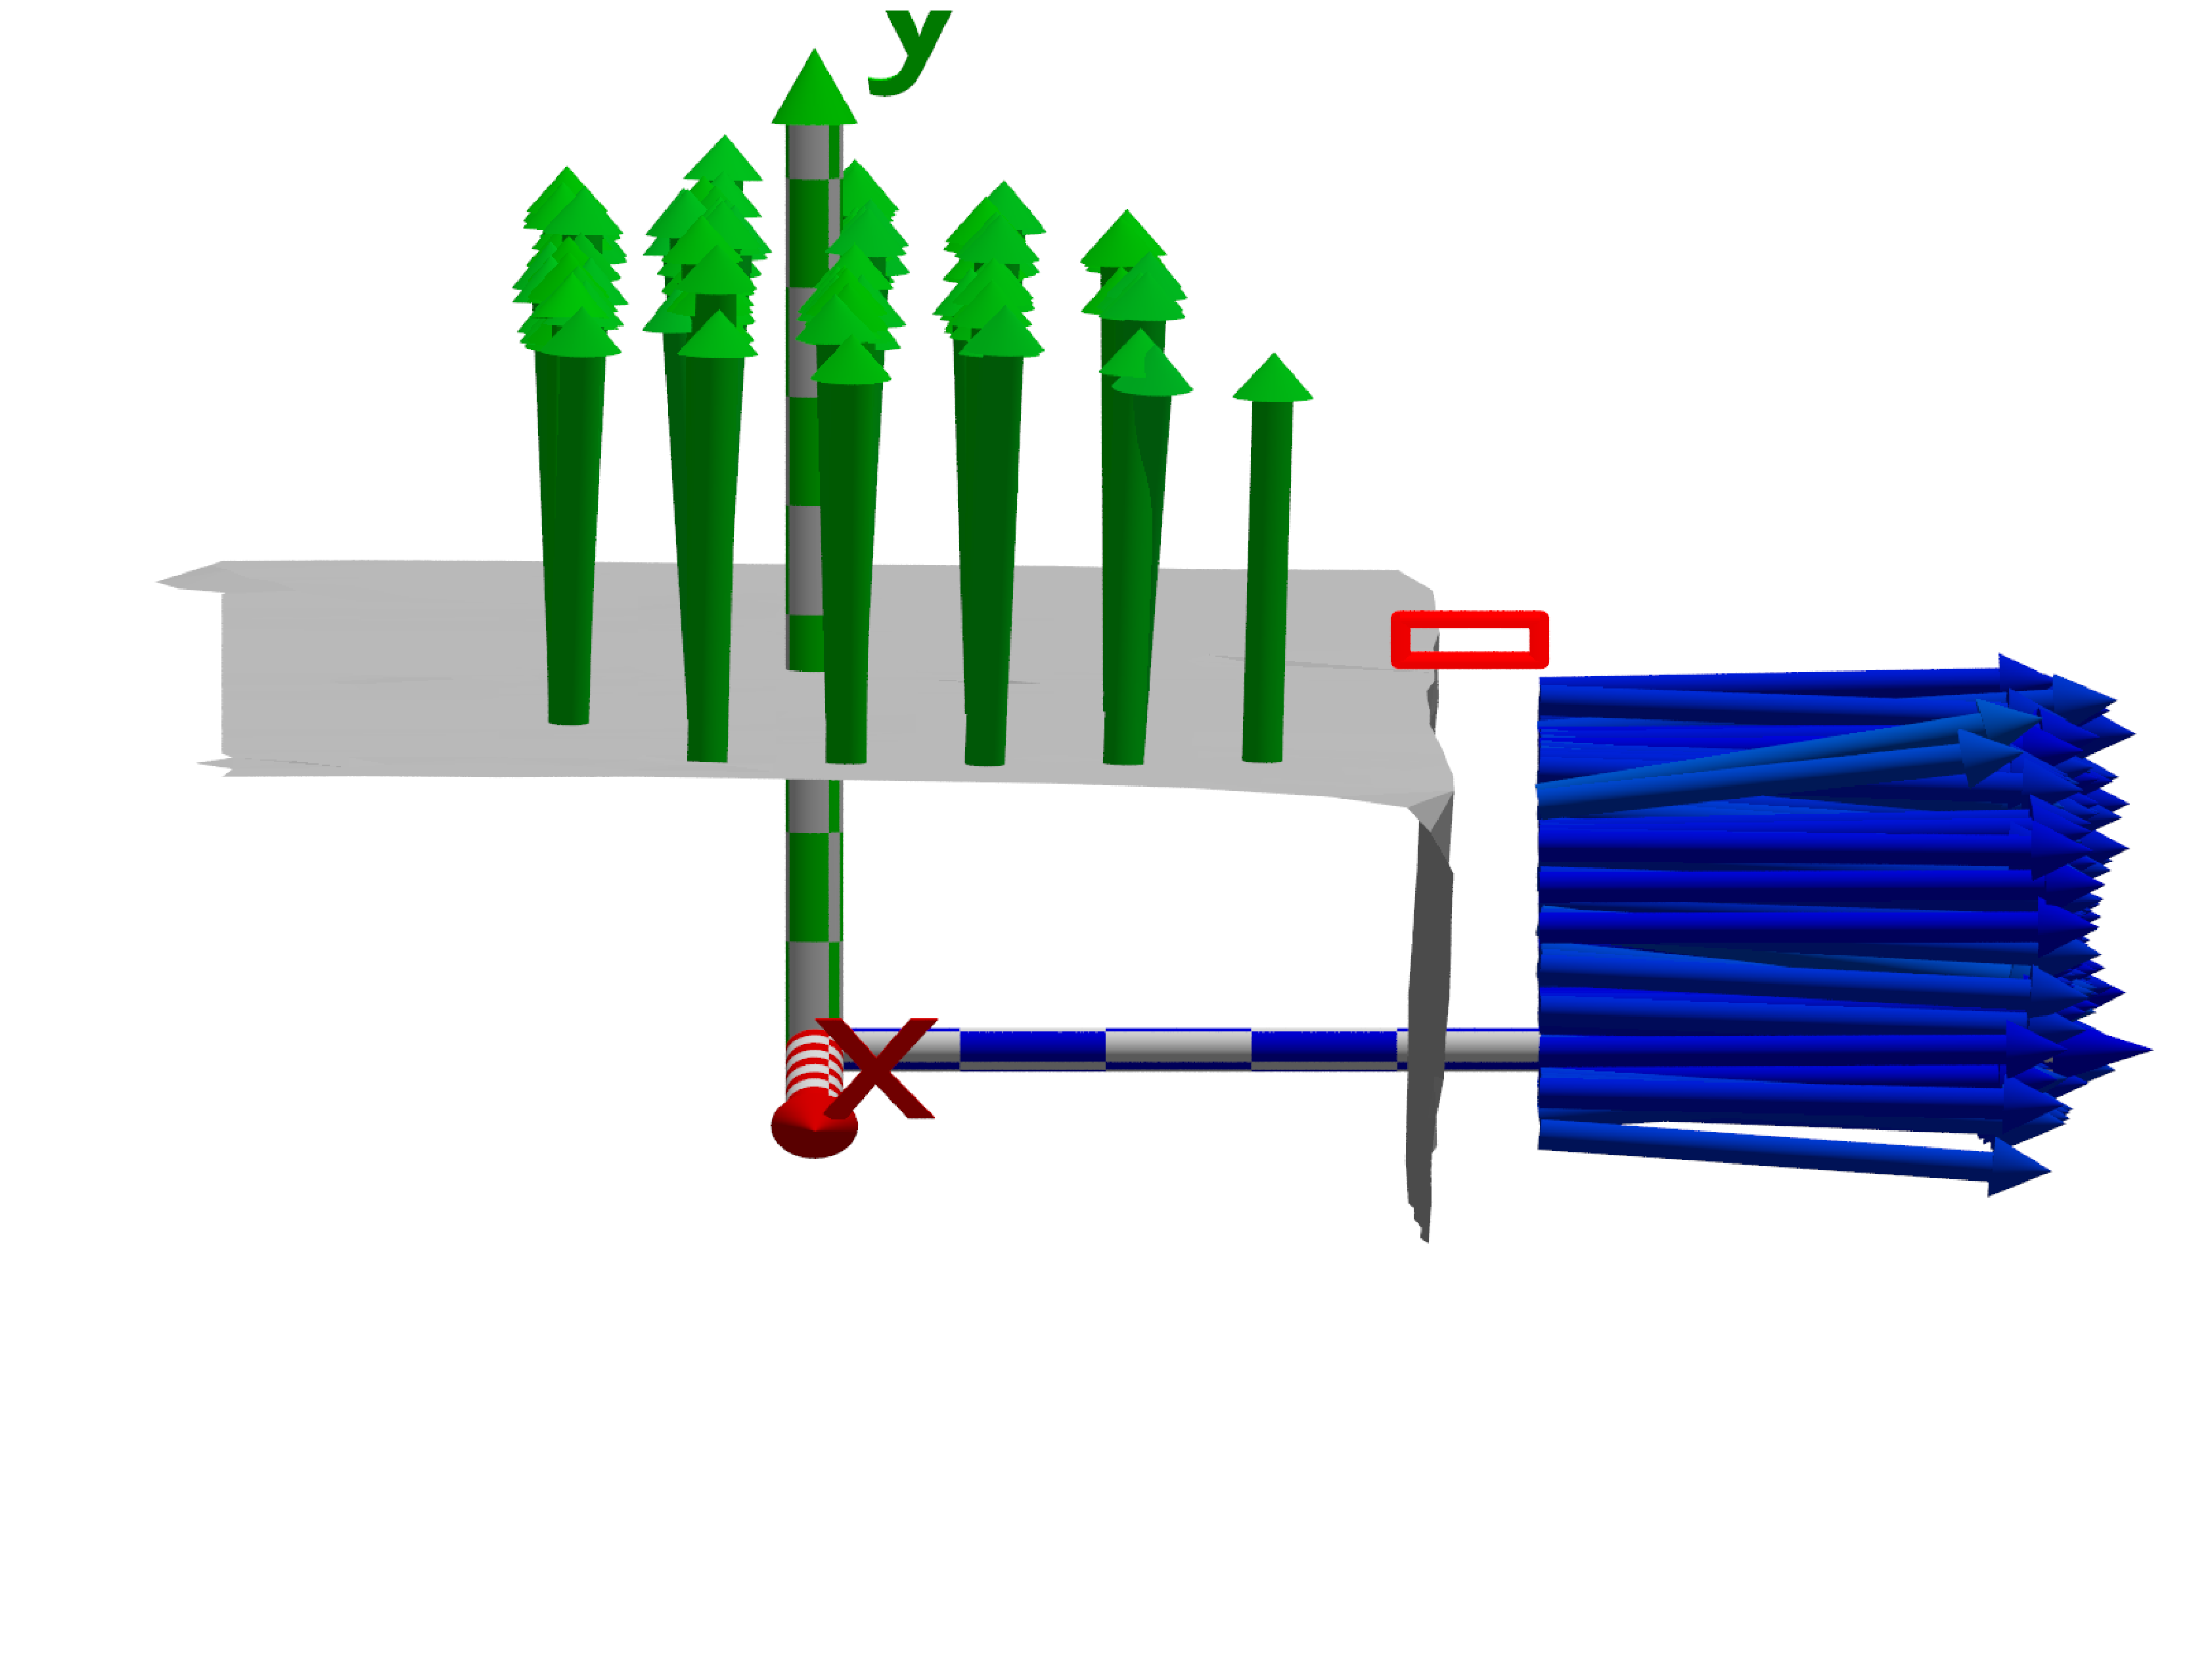
\includegraphics[width=0.25\linewidth]
                 {images/setA.crop2.religrad.new.eps}\label{fig:setA.crop1.religrad}}
\caption{The gradients generated on a portion of the \textit{engine cylinder} dataset, the cyan inset  in figure~\ref{fig:grad-1} shows context of where the dataset is extracted from. Figure~\ref{fig:setA.crop1.algo1} shows the gradients at vertices marked reliable by Algorithm~\ref{alg:curved}. Figure~\ref{fig:setA.crop1.algo2} shows the result of Algorithm~\ref{alg:phi2}, Figure~\ref{fig:setA.crop1.findReliable} shows results of Algorithm~\ref{alg:extend}. Finally, Figure~\ref{fig:setA.crop1.religrad} shows gradients marked reliable by \protect\ReliGrad. The red rectangle shows the proportional size of unit grid cube, the spacing is the Z axis is 0.68 compared to 0.27 for other axes. } 
\label{fig:setA.crop1.grads}
\end{figure}
\begin{figure}[htb]
    \centering
    \subfloat[Single image slice, original machine part]{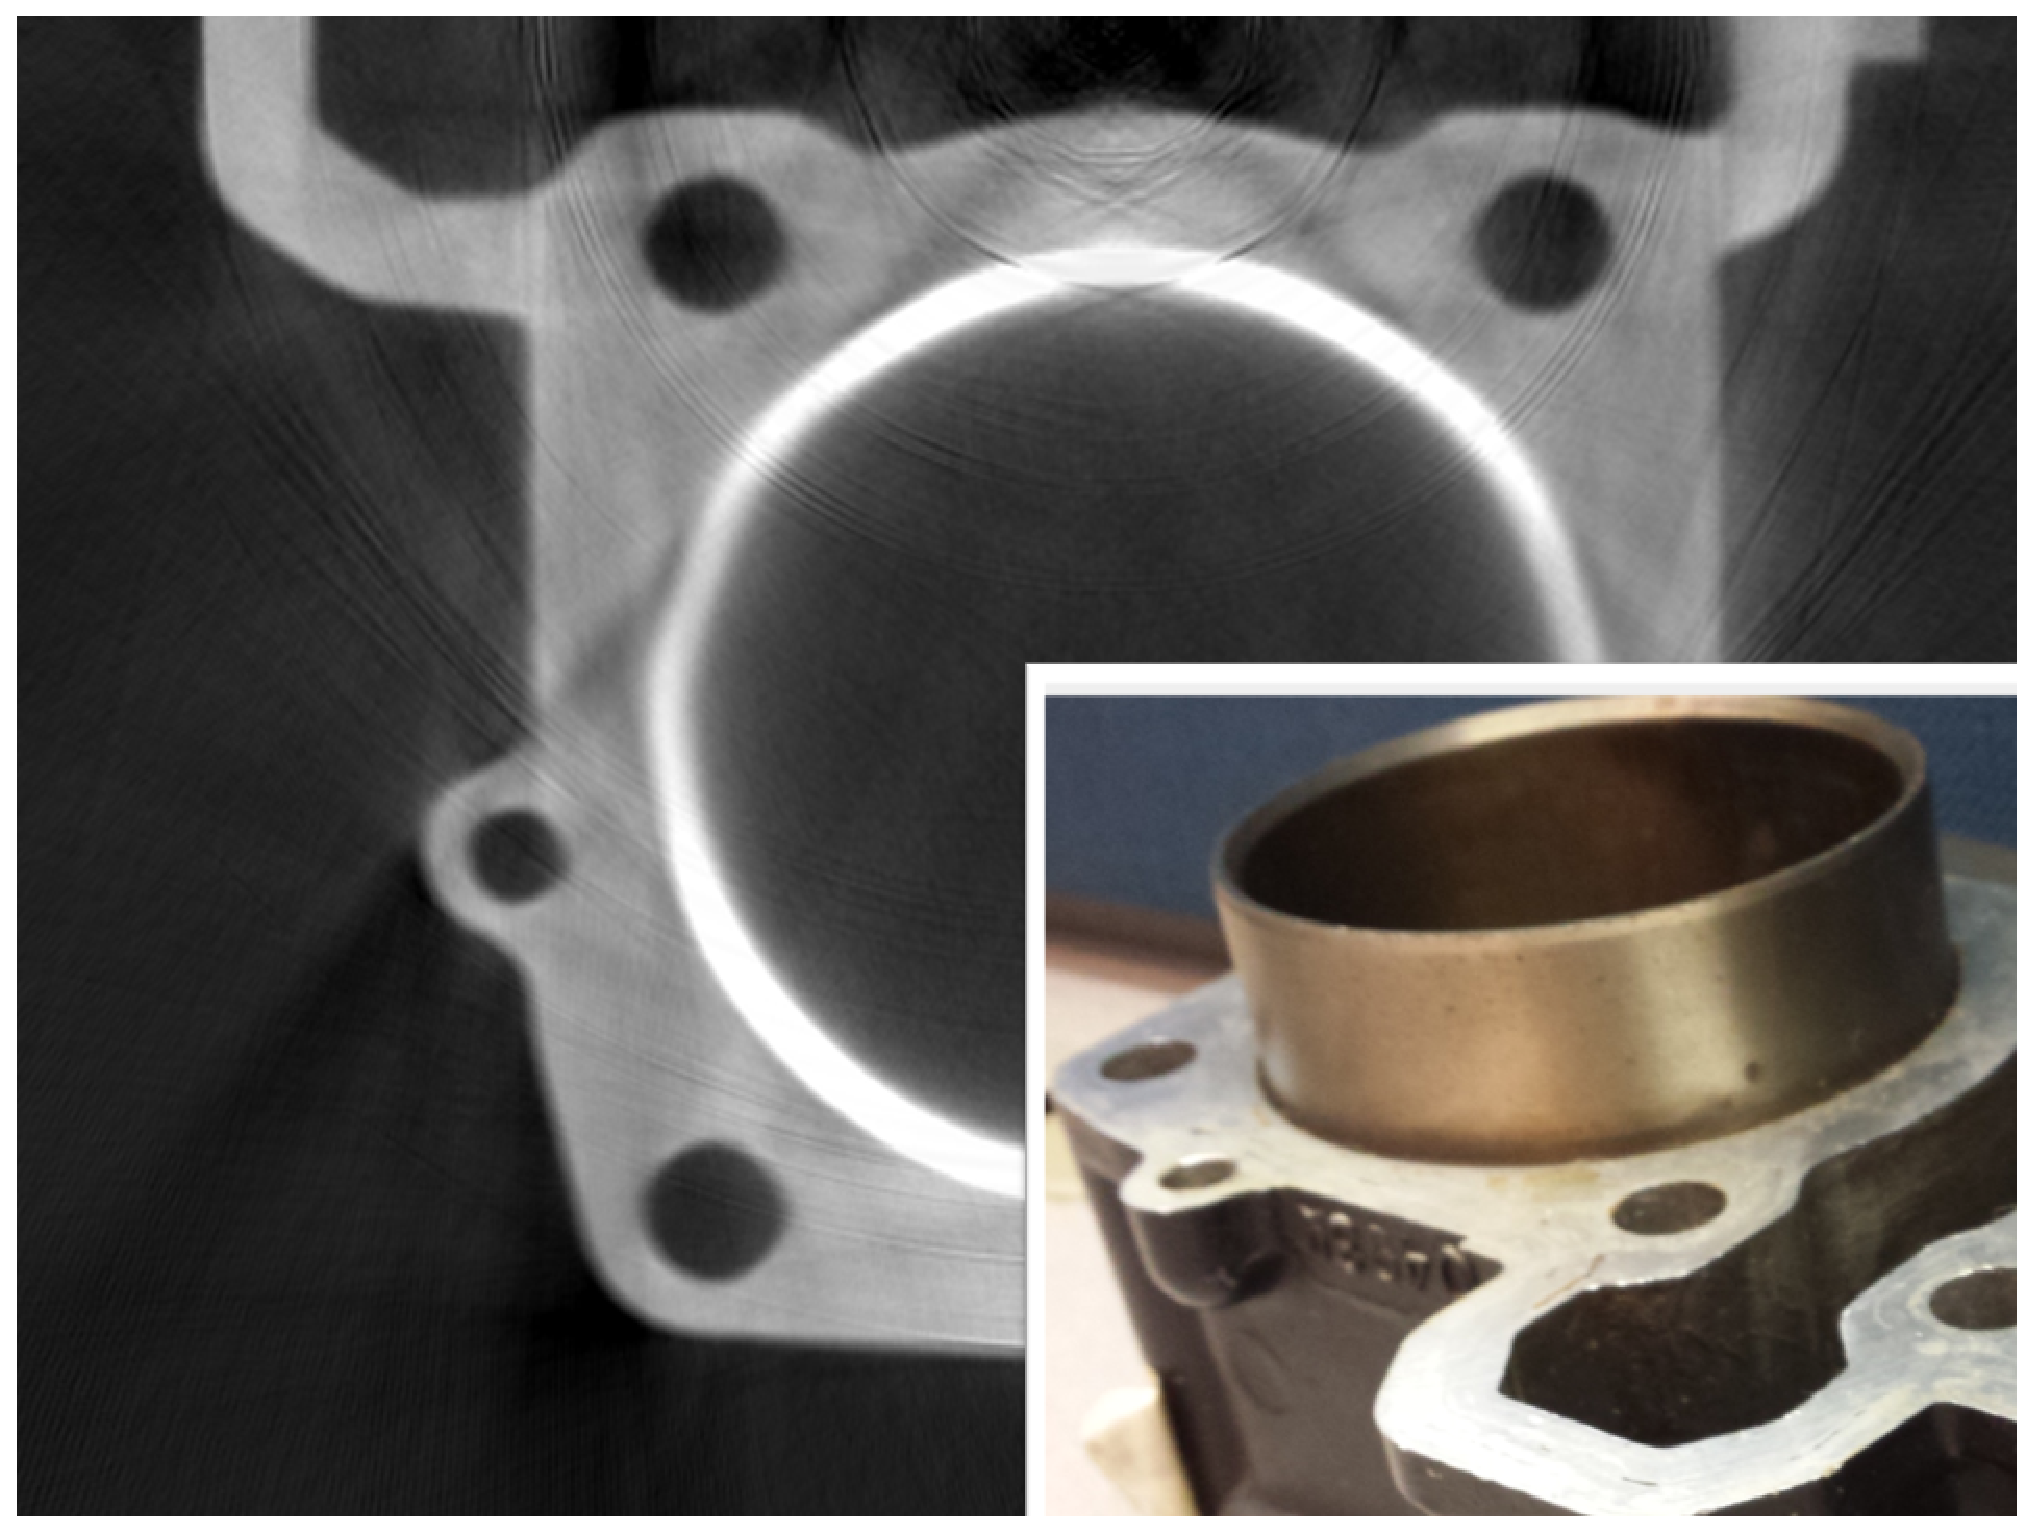
\includegraphics[width=0.3\linewidth ]{images/cly_sleeve.1.eps}\label{fig:setA.crop1.1}}
    \subfloat[Sharp Isosurface]{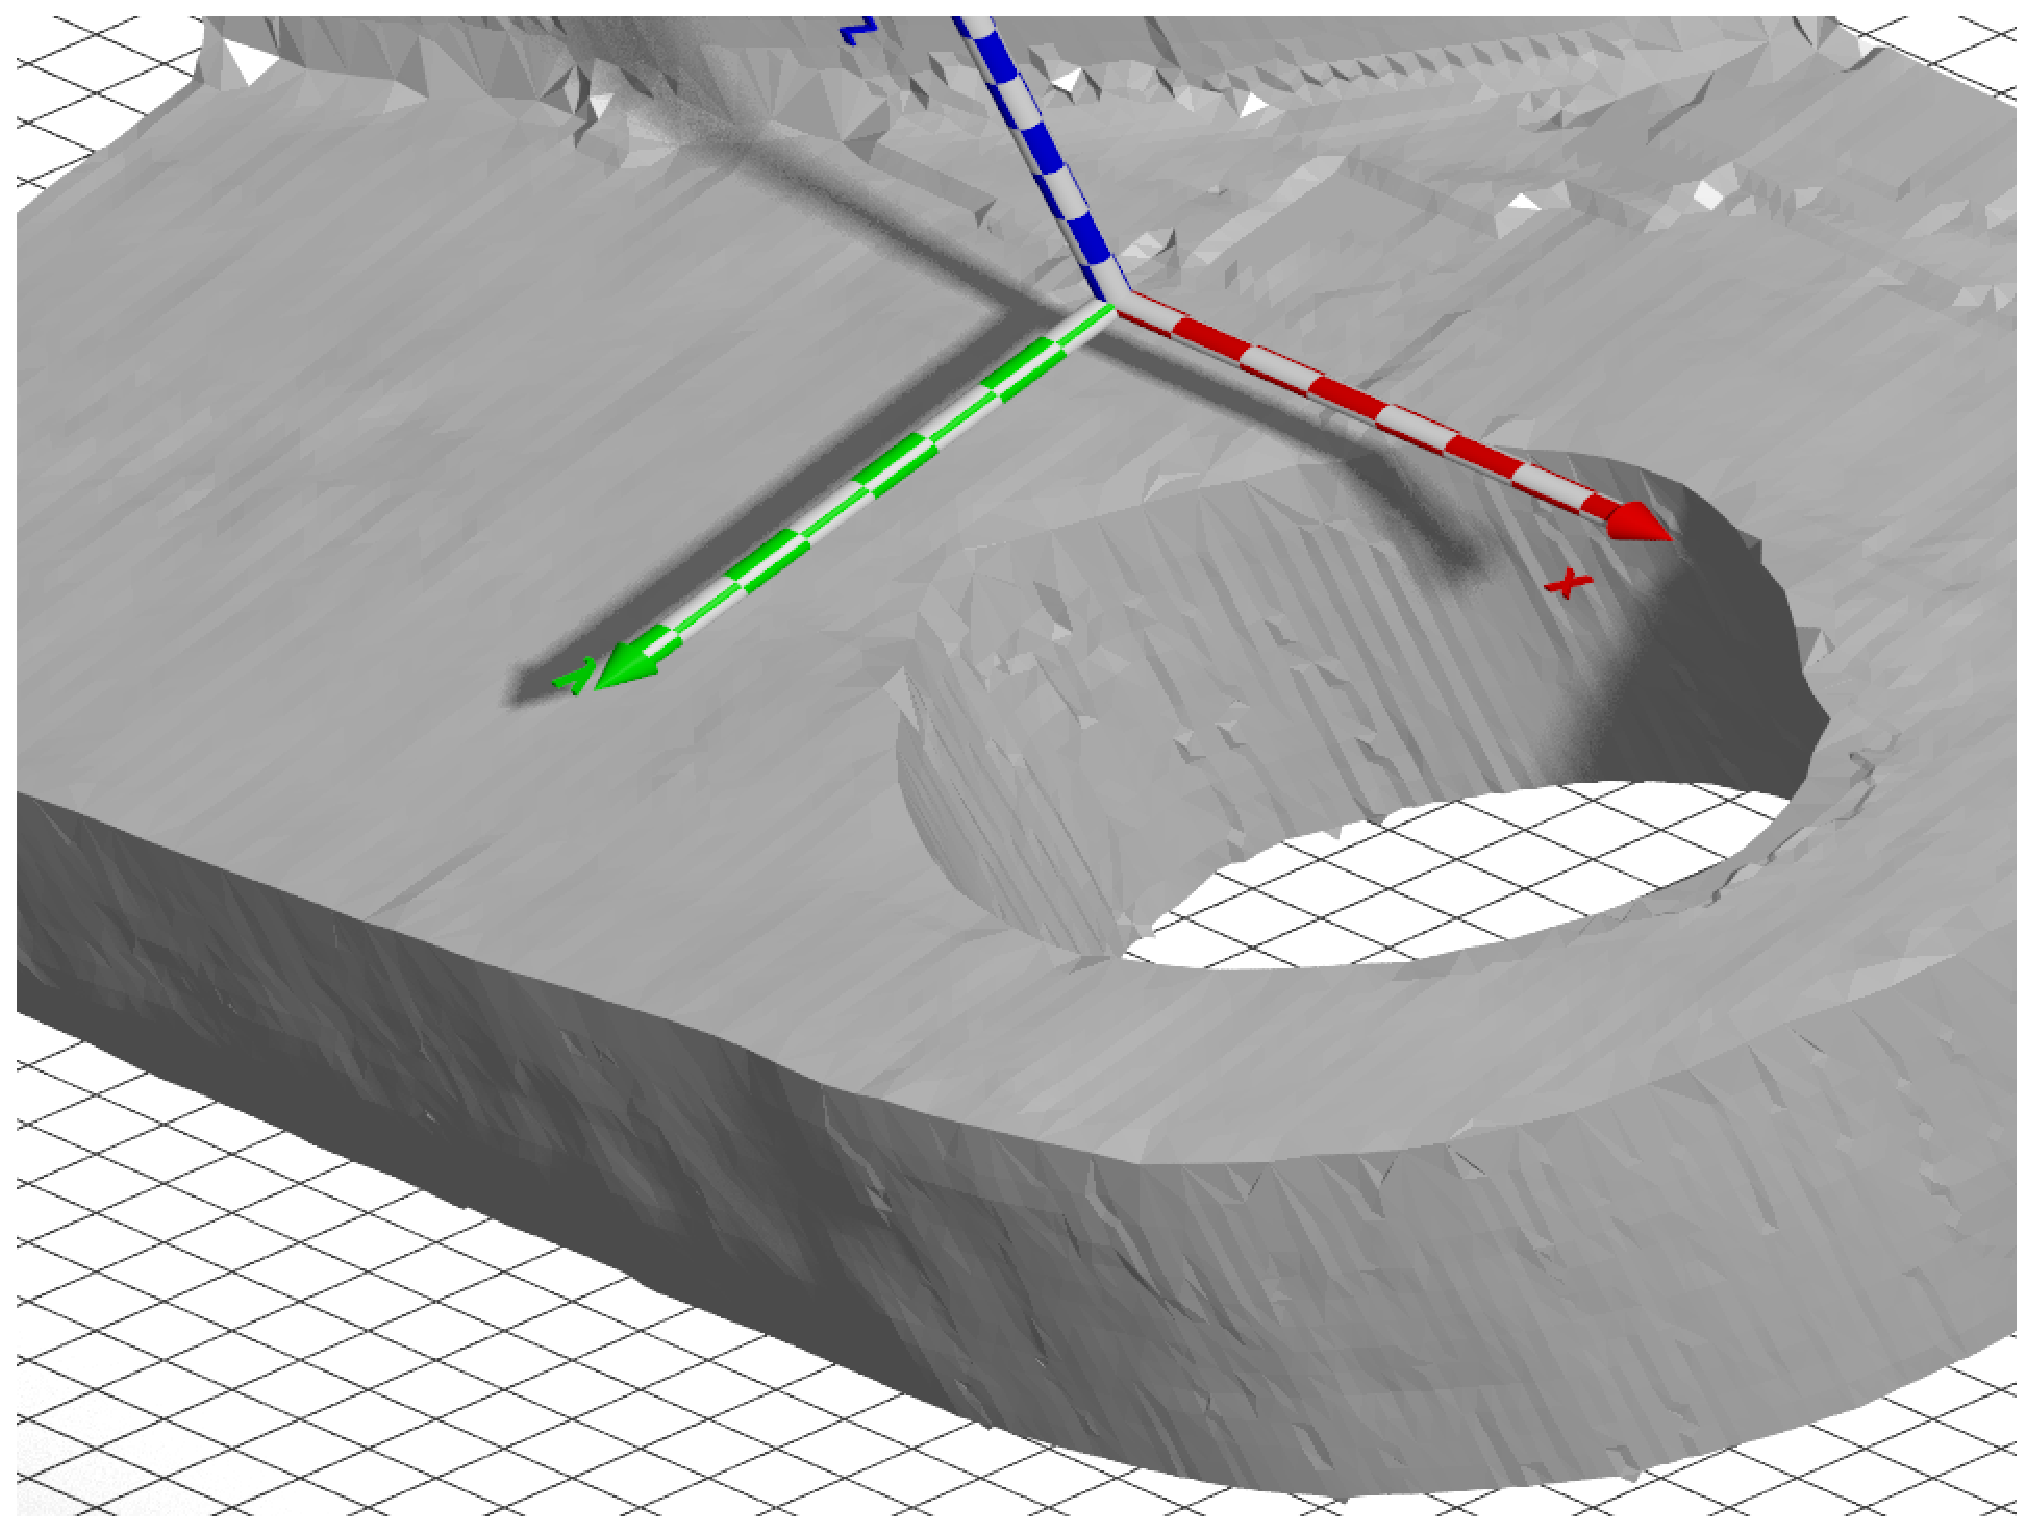
\includegraphics[width=0.3\linewidth]
        {images/setA.rendering.eps}\label{fig:setA.crop1.2}}
    \subfloat[Sparse feature points]{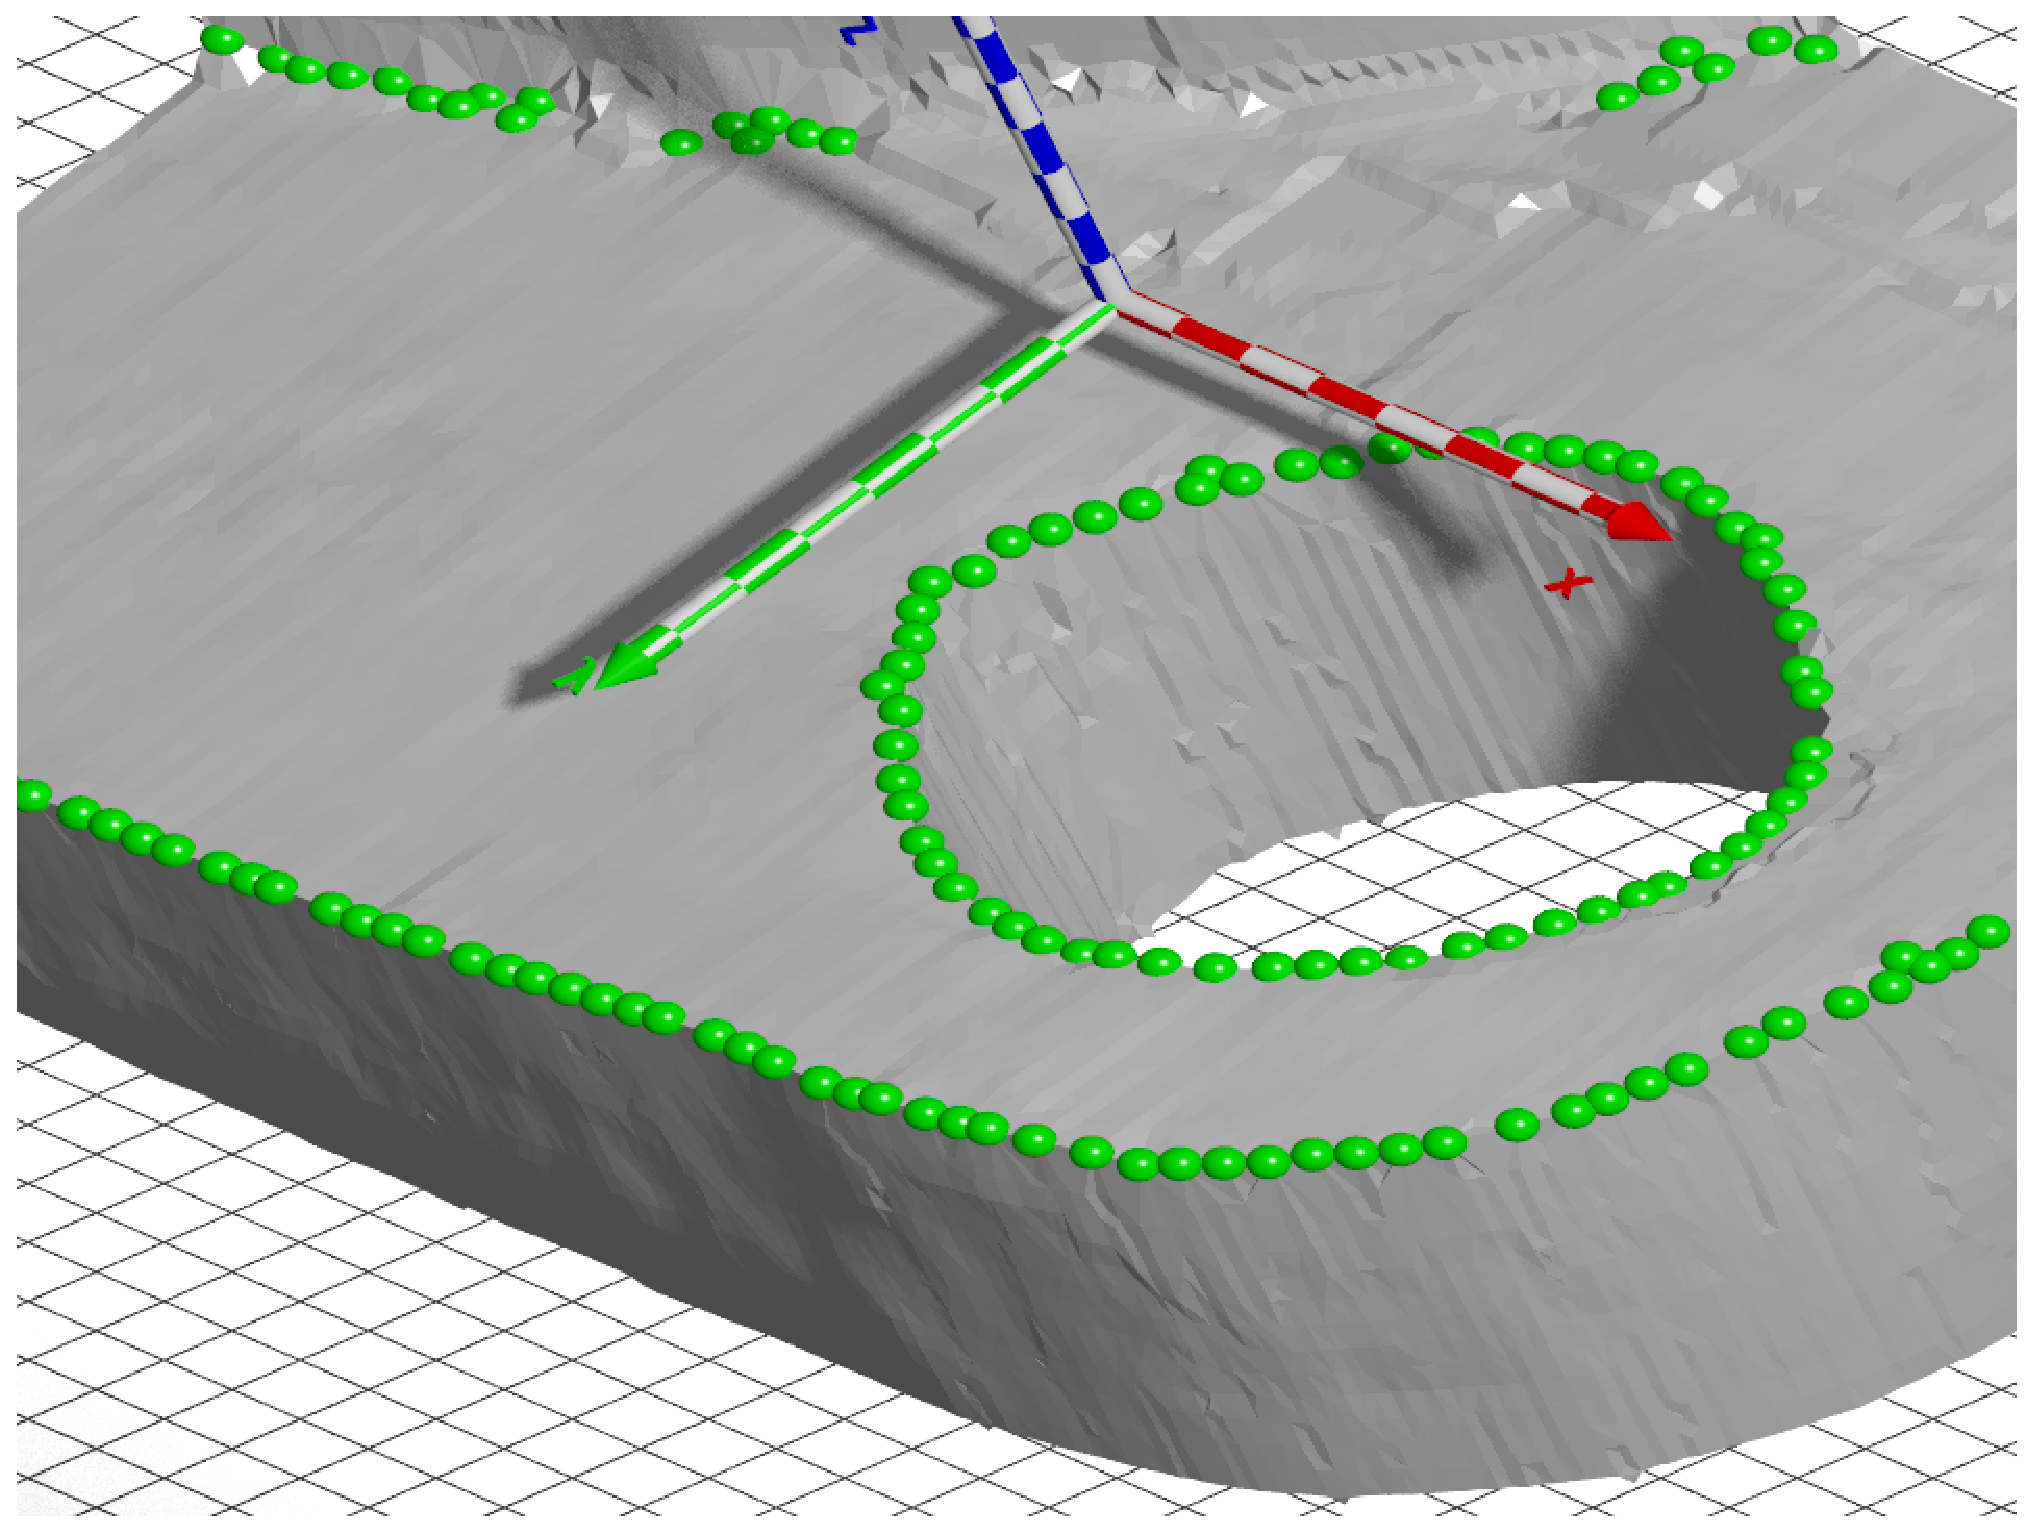
\includegraphics[width=0.3\linewidth]
        {images/setA.rendering2.eps}\label{fig:setA.crop1.3}}
    \caption{\textit{Engine Cylinder} dataset.~\protect\subref{fig:setA.crop1.1} a slice of the original CT image, note the streaking artifacts introduced during the scanning process.
    The inset shows the original machine part. Figure \protect\subref{fig:setA.crop1.2},~\protect\subref{fig:setA.crop1.3}, shows the sharp mesh, and the extracted sparse feature points.}
    \label{fig:setA.crop1}
\end{figure}
% Please add the following required packages to your document preamble:
% \usepackage{multirow}
We also evaluate our algorithm on a number of industrial CT data sets (table~\ref{table:ictDataInfo}). 

\textbf{Description:} Figure~\subref*{fig:CMM:b} shows an isosurface of the CMM dataset. Coordinate Measuring machine (CMM) is commonly used to calibrate CT devices. Figure~\subref*{fig:CMM:a} shows a single slice along the XY plane. CMM has larger 0.31 spacing along the Z axis, and uniform 0.2 in X,Y axis.
Figure~\subref*{fig:setA.crop1.1} shows a single slice of the output of the CT scan of the \textit{engine cylinder} dataset. It also shows the streaking affects introduced in the scanning process. The inset shows the original dataset. It is a part of a Motor Cycle Engine.
Figure~\subref*{fig:intake:b} shows an isosurface of the intake dataset, along with a single slice along the XY plane, it is part of an engine intake valve. Figure~\subref*{fig:socket:a} shows the socket dataset, it is a part of a 440volt converter. Figure~\subref*{fig:socket:c} shows a single slice along the YZ plane using the hsv color scale. Table~\ref{table:ictDataInfo} provides the size and spacing info on all these data sets. 

\textbf{Reliable Gradients} 
Figure~\ref{fig:setA.crop1.cdiff} shows the central difference gradients at all grid vertex location around an edge of the \textit{engine cylinder} dataset.
Figure~\ref{fig:grad-1} provides context. The length of the vectors are proportional to the magnitude of the gradients. Note, how the gradients quickly fall off. The problem is more acute, along the Z-Axis. 
The magnified portion shows that there are about two good columns of gradients after which the gradient magnitude becomes too small and the gradient directions meaningless. 
Figure~\subref*{fig:setA.crop1.algo1},~\subref*{fig:setA.crop1.algo2} show the results of Algorithm ~\ref{alg:curved} and Algorithm ~\ref{alg:phi2} respectively. Unlike the simulated datasets, almost no gradients along the Z axis are marked as reliable. This shows the need for dividing the vertex set into tangential and orthogonal neighbor sets. This lead us to Algorithm~\ref{alg:religrad}. Figure~\subref*{fig:setA.crop1.findReliable} shows the corresponding gradients of the \FindReliable technique. Figure~\subref*{fig:setA.crop1.religrad} shows the~\ReliGrad gradients. For reference, figure~\ref{fig:grad-1} shows the Central Difference gradients. 
  
\subsection{Visualization}
\subsubsection{Sparse feature point detection}
\label{sec:sparsePointExtraction}
Once we have a set of reliable gradients in a neighborhood of a grid vertex we can use the technique in section ~\ref{sec:grad_select} to select a set of gradients in a neighborhood and then use the technique described in section~\ref{sec:computeSharpPoints} to compute sharp feature points. Figure~\subref*{fig:setA.crop1.mesh.2} shows the generated points for a portion of the \textit{ engine cylinder} dataset. 
The generated isovertices, one for each grid cube, is  noisy.

Starting from these isovertices, we utilize the merging technique in MergeSharp~\cite{bw-cisec-13} to compute a set of sparse feature points. Figure~\subref*{fig:setA.crop1.mesh.3} shows the sparse feature points.

\subsubsection{Point Skeleton Visualization}
The sparse feature vertices are used to create a sharp feature point skeleton. The point set skeleton is visualized for the synthetic dataset in figure~\ref{fig:SynData}. The number of large Eigenvalues determines if the sharp feature is on an edge or on a corner. Points on the edges are marked in green and corner points in red.
The skeleton is correctly extracted on challenging non-axis aligned datasets. We also do well on  acute and obtuse angles (figure~\subref*{fig:cannon},~\subref*{fig:cone}).

Figure~\subref*{fig:setA.crop1.3} shows the extracted sparse point skeleton of a part of the \emph{engine cylinder} dataset. Figure~\subref*{fig:CMM:c} shows the point skeleton the CMM dataset. Figure~\subref*{fig:socket:b} shows the point skeleton of the \emph{socket} dataset.
 \begin{wrapfigure}{r}{0.5\linewidth}
    \centering
    \subfloat[Annulus]{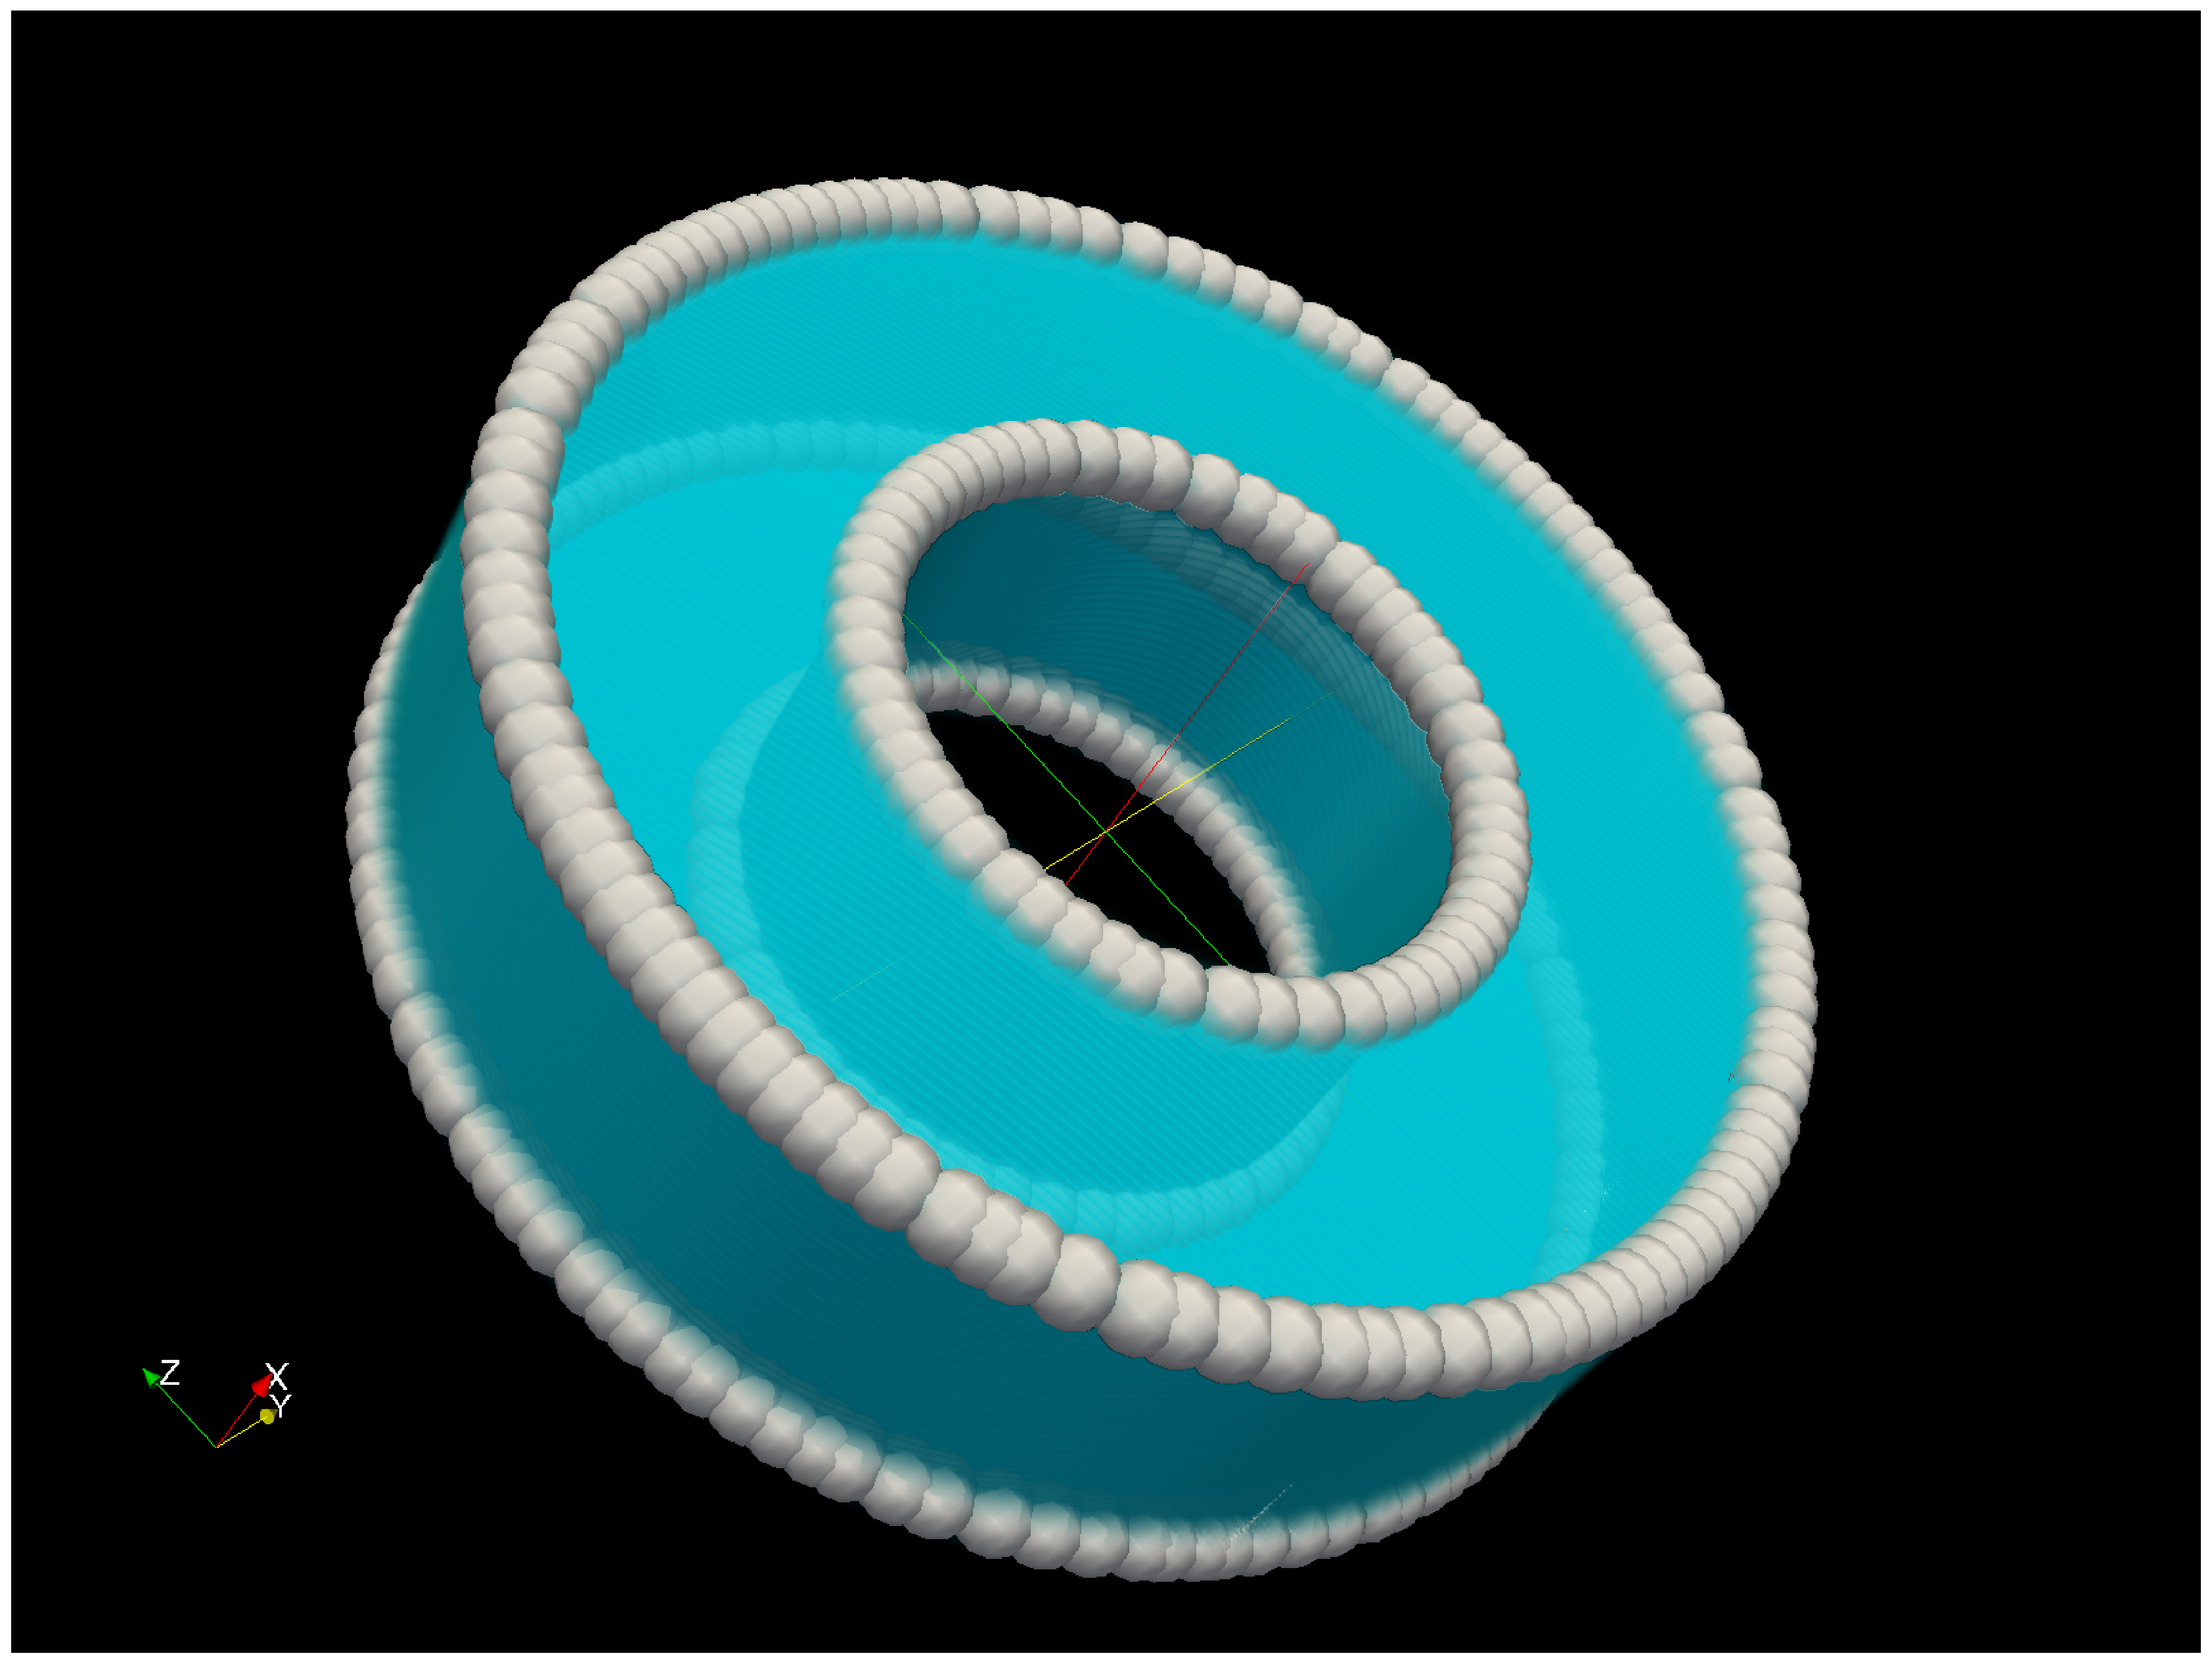
\includegraphics[width=0.5\linewidth]{images/volren.ann.eps}\label{fig:paraview:a}}
    \subfloat[Twocube]{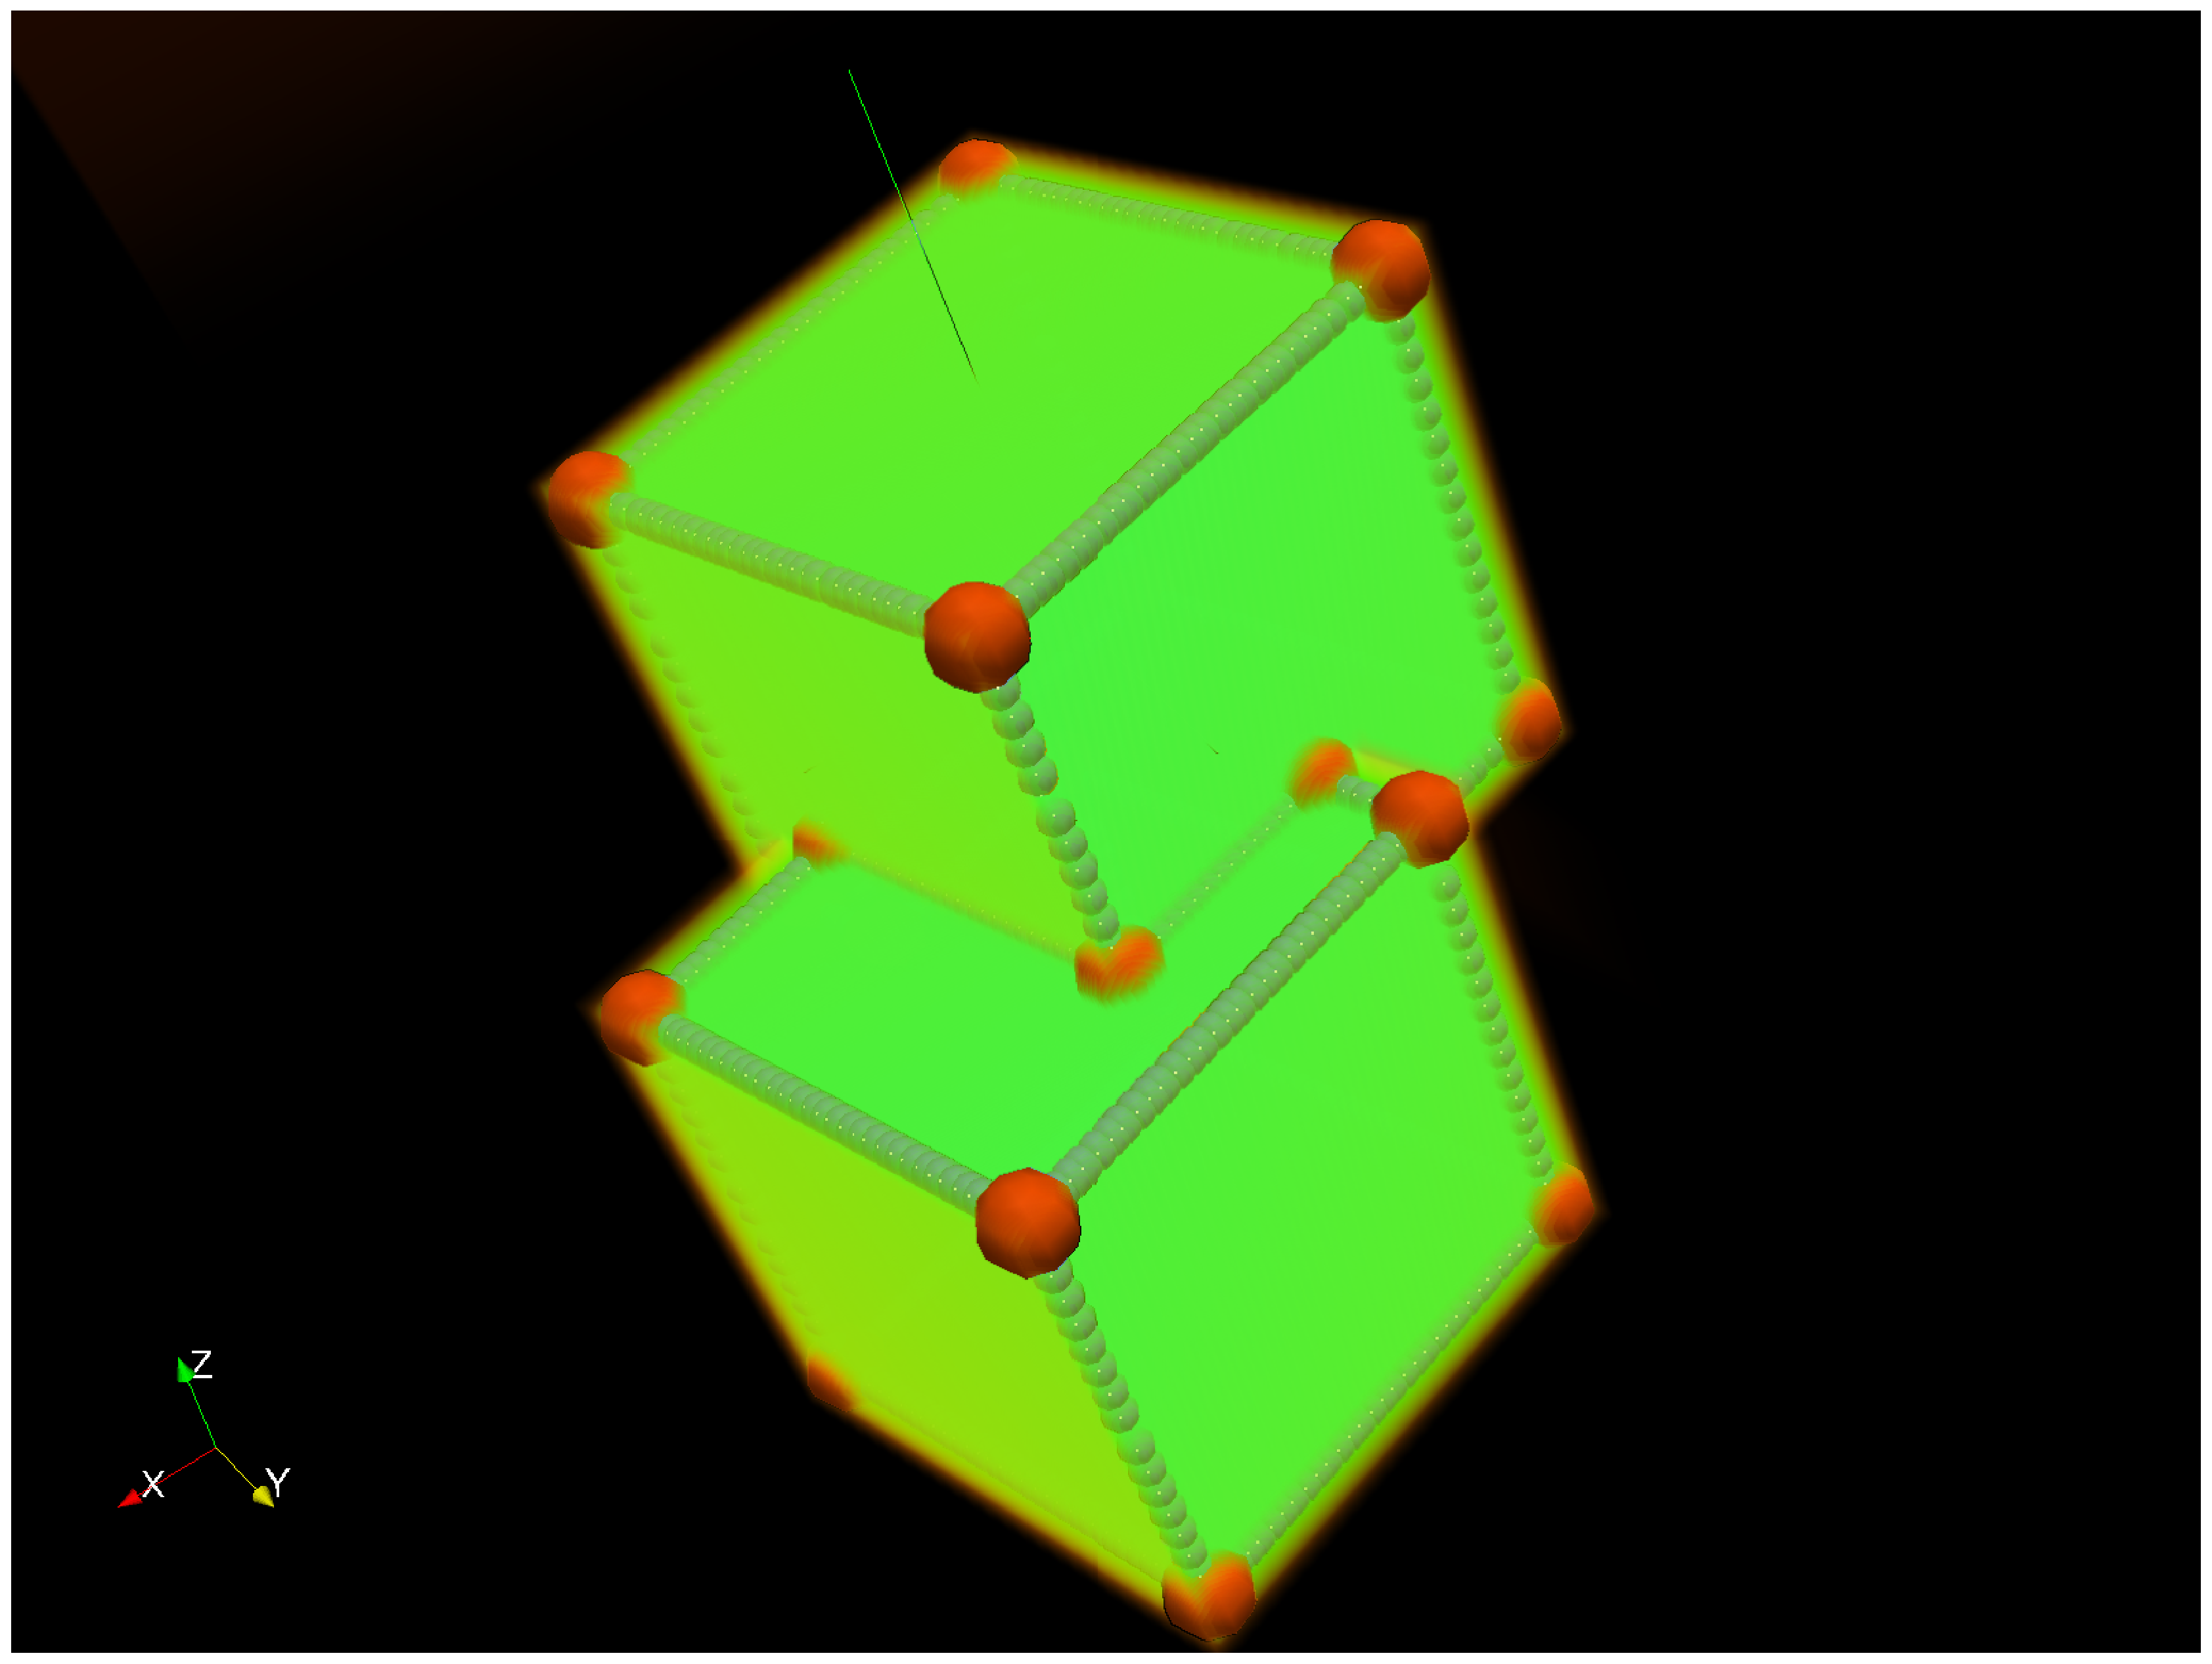
\includegraphics[width=0.5\linewidth]{images/volren.twocube.eps}\label{fig:paraview:b}}\vspace {-3mm}
    \caption{Integrating results into ParaView~\cite{Ayachit2015}. Volume rendering of the Annulus and TwoCube dataset, overlay-ed with sparse feature skeleton.}
    \label{fig:paraview}
\end{wrapfigure}

%\begin{figure}[h]
%    \centering
%    \subfloat[Annulus]{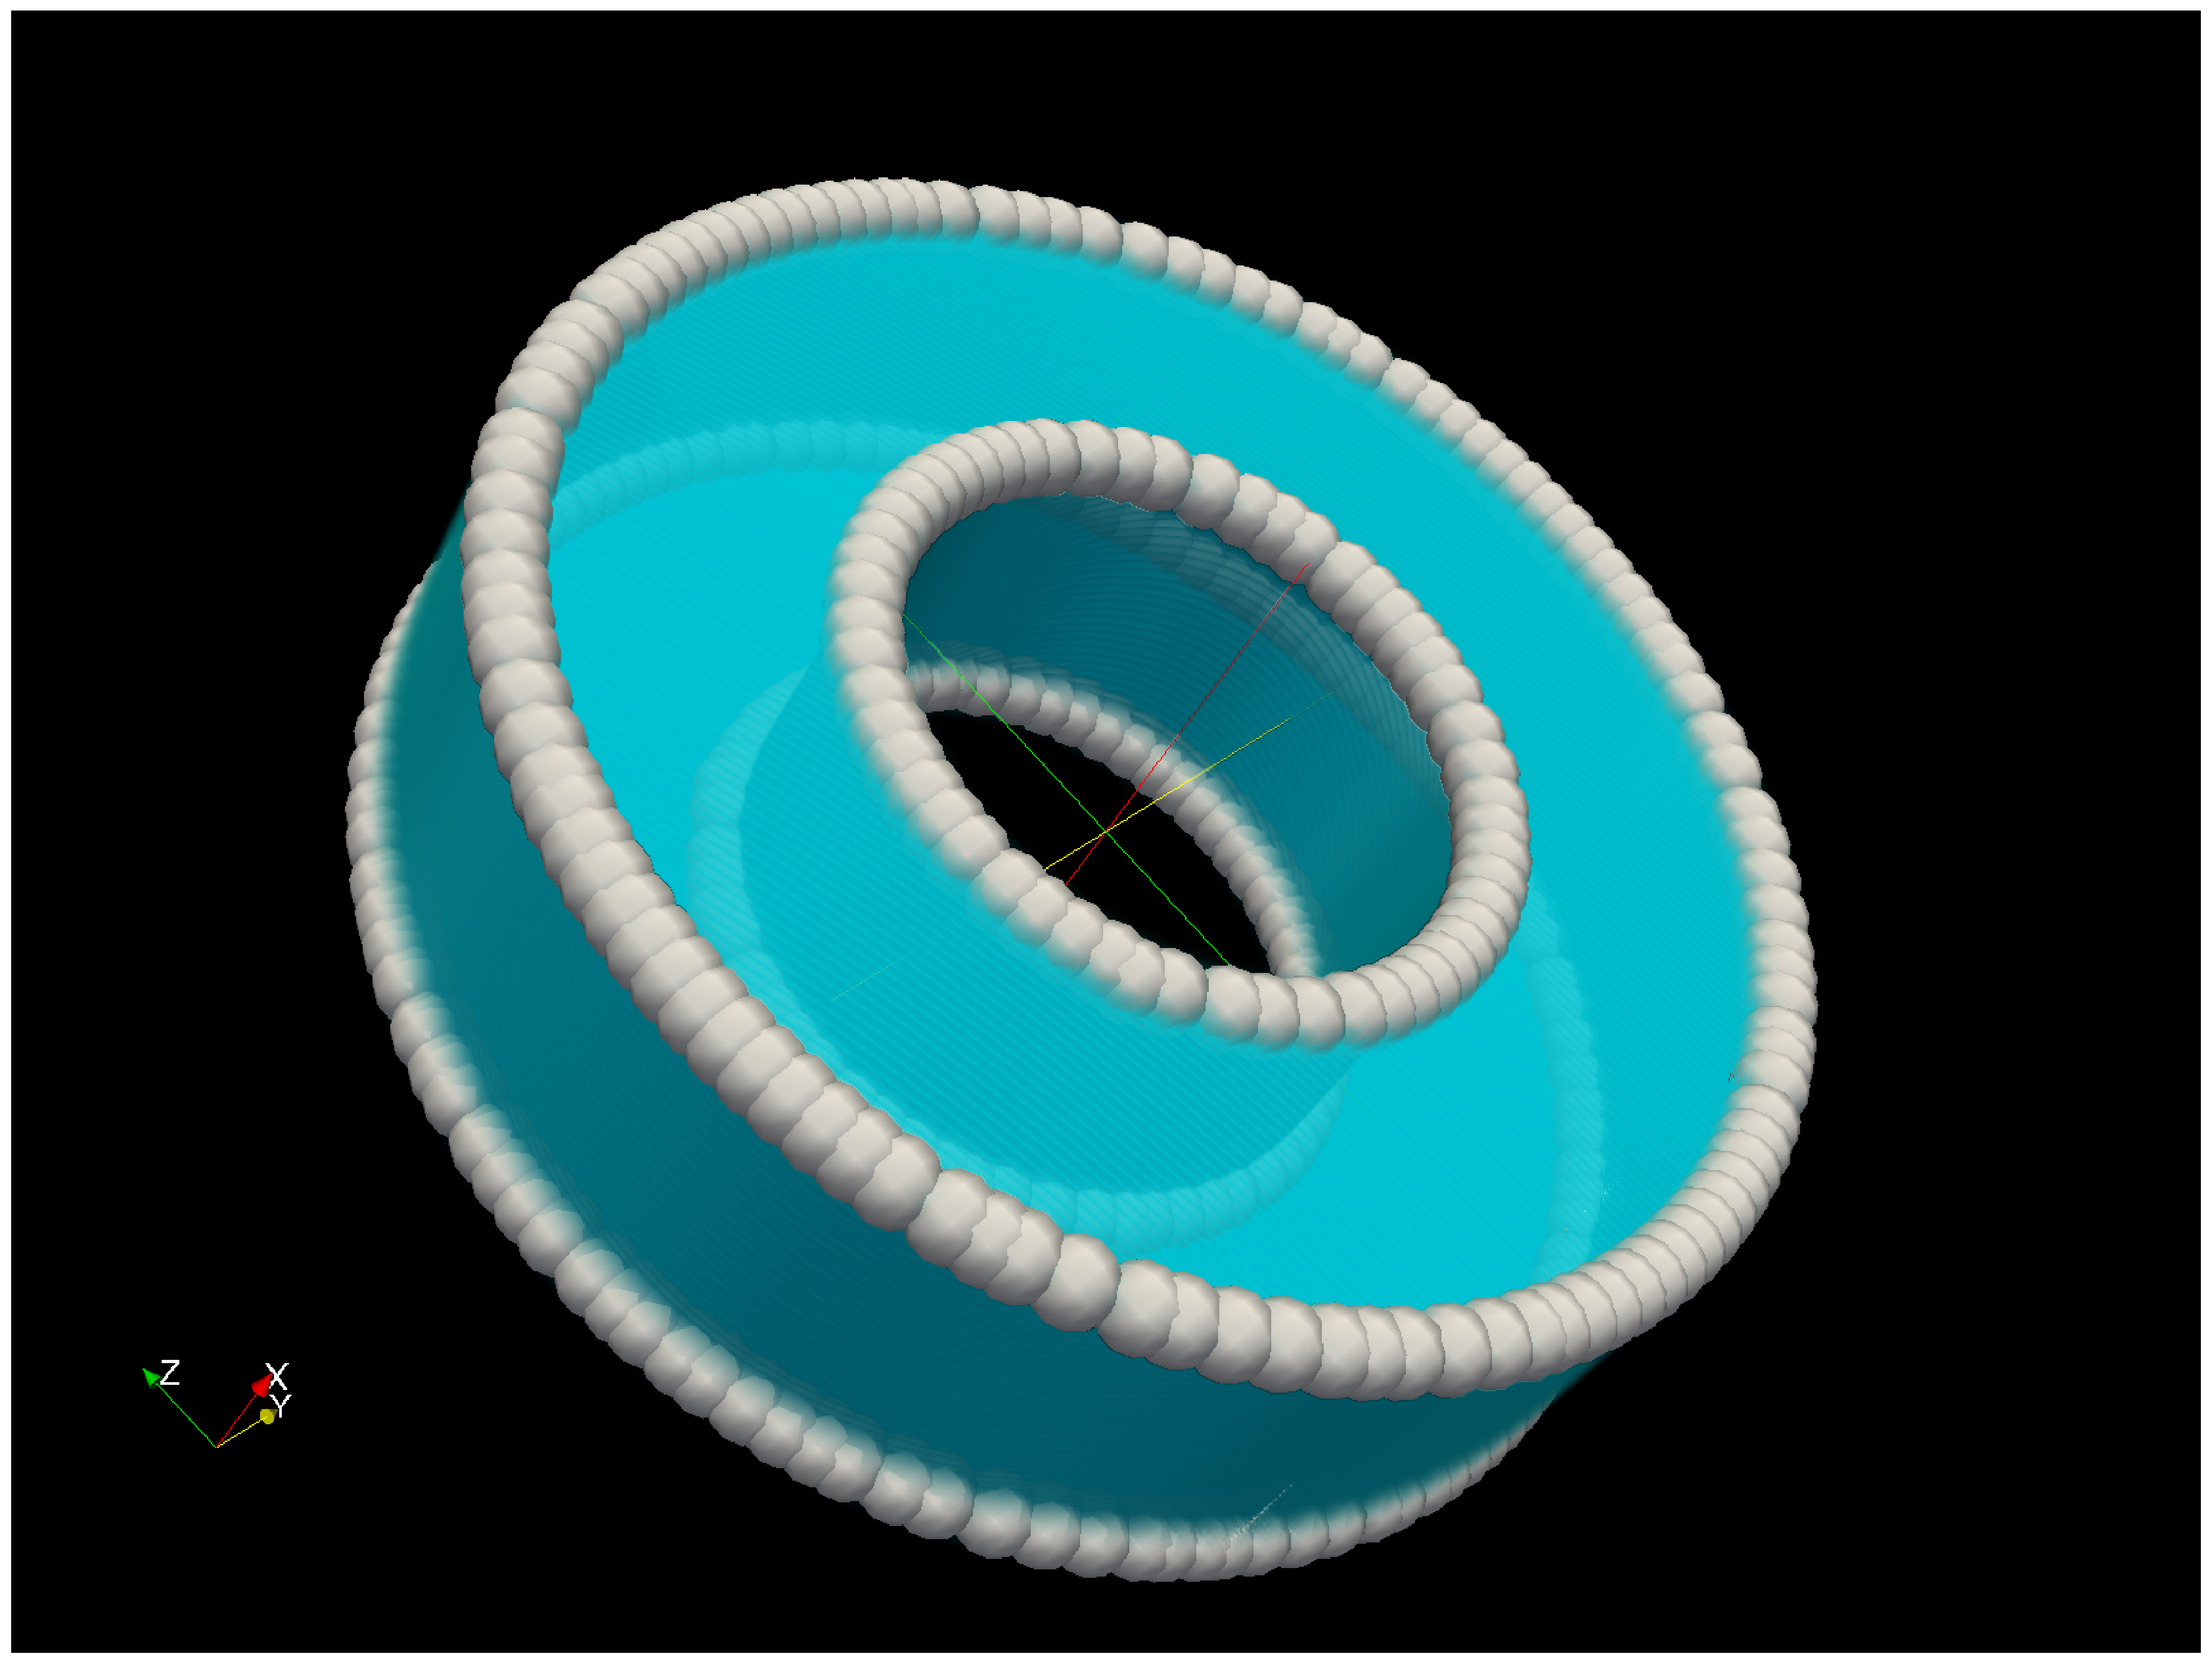
\includegraphics[width=0.3\linewidth]{images/volren.ann.eps}\label{fig:paraview:a}}
%    \subfloat[Twocube]{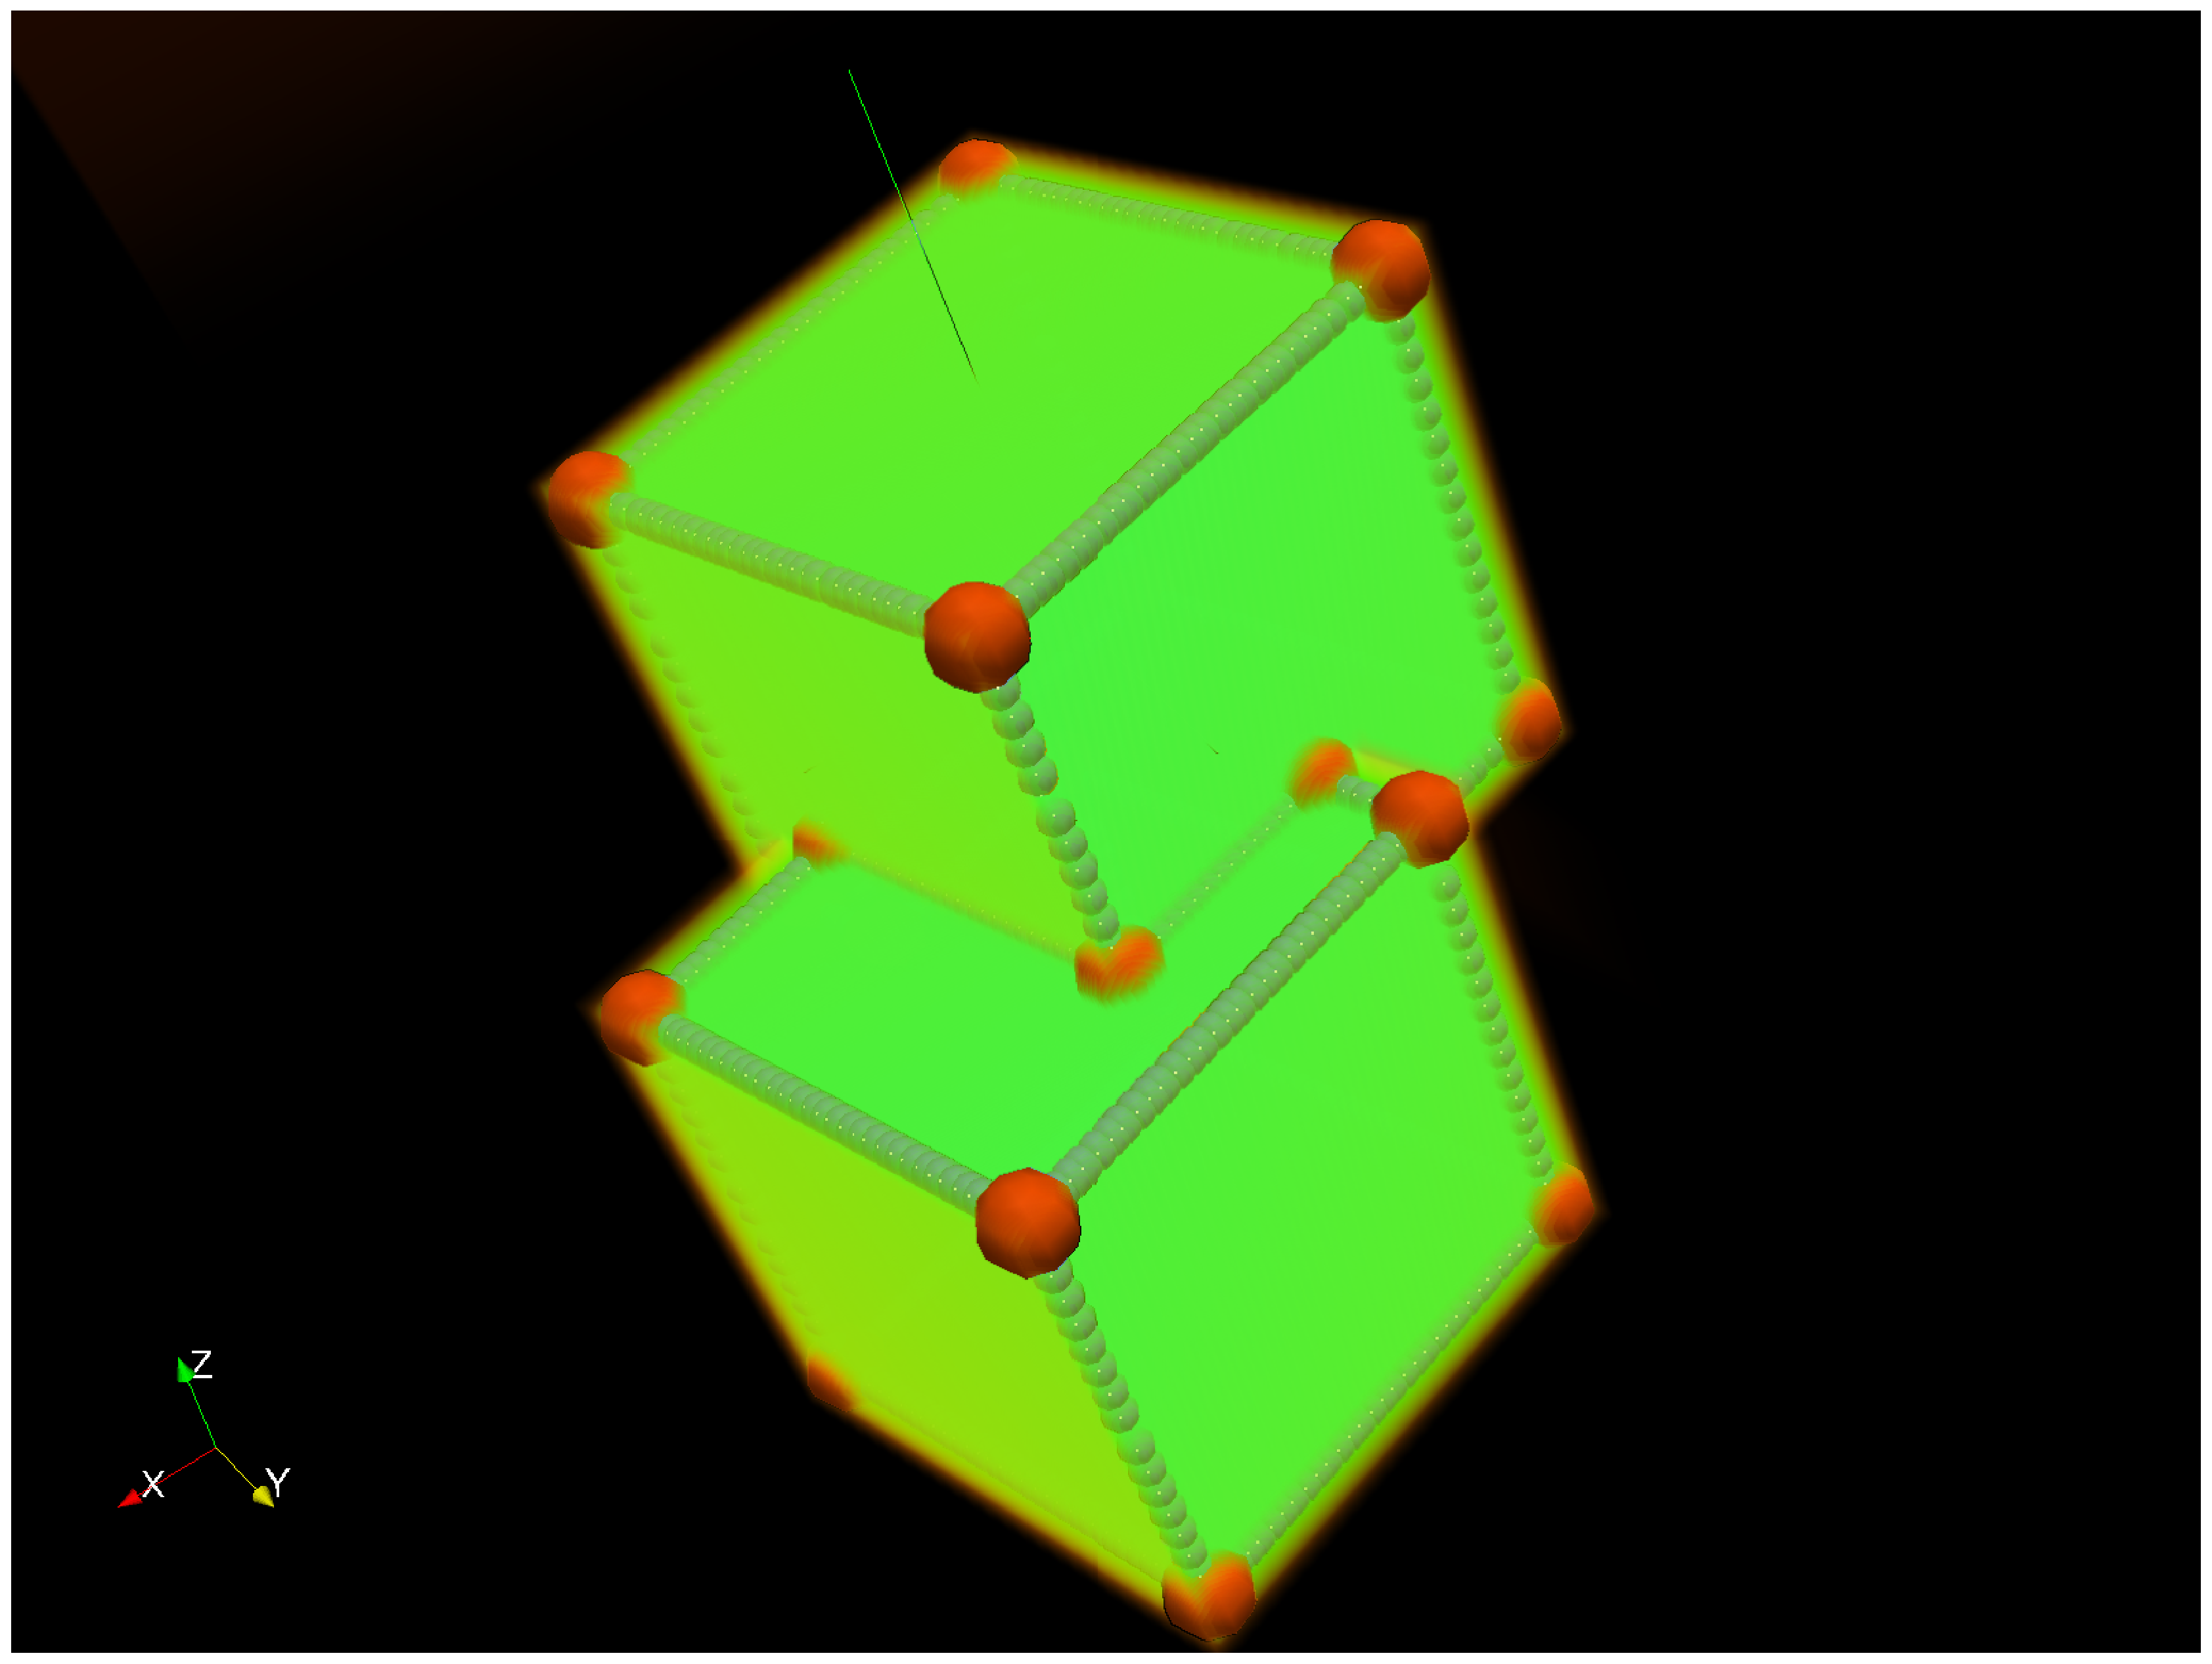
\includegraphics[width=0.3\linewidth]{images/volren.twocube.eps}\label{fig:paraview:b}}
%    \caption{Integrating results into ParaView~\cite{Ayachit2015}. Volume rendering of the Annulus and TwoCube dataset, overlay-ed with sparse feature skeleton.}
%    \label{fig:paraview}
%\end{figure}
%
Apart from direct point visualization,  The extracted feature points can be quickly integrated into commonly used frameworks. For example, figure~\subref*{fig:paraview:a},~\subref*{fig:paraview:b} shows the volume rendering of the datasets using ParaView~\cite{Ayachit2015}, overlay-ed  with the detected edge and corner points. The simple addition of the edge points makes the rendering more comprehensible.
\begin{figure}
    \centering
    \subfloat[Single XY slice, hsv color scale. Intensity range is 0-41000]{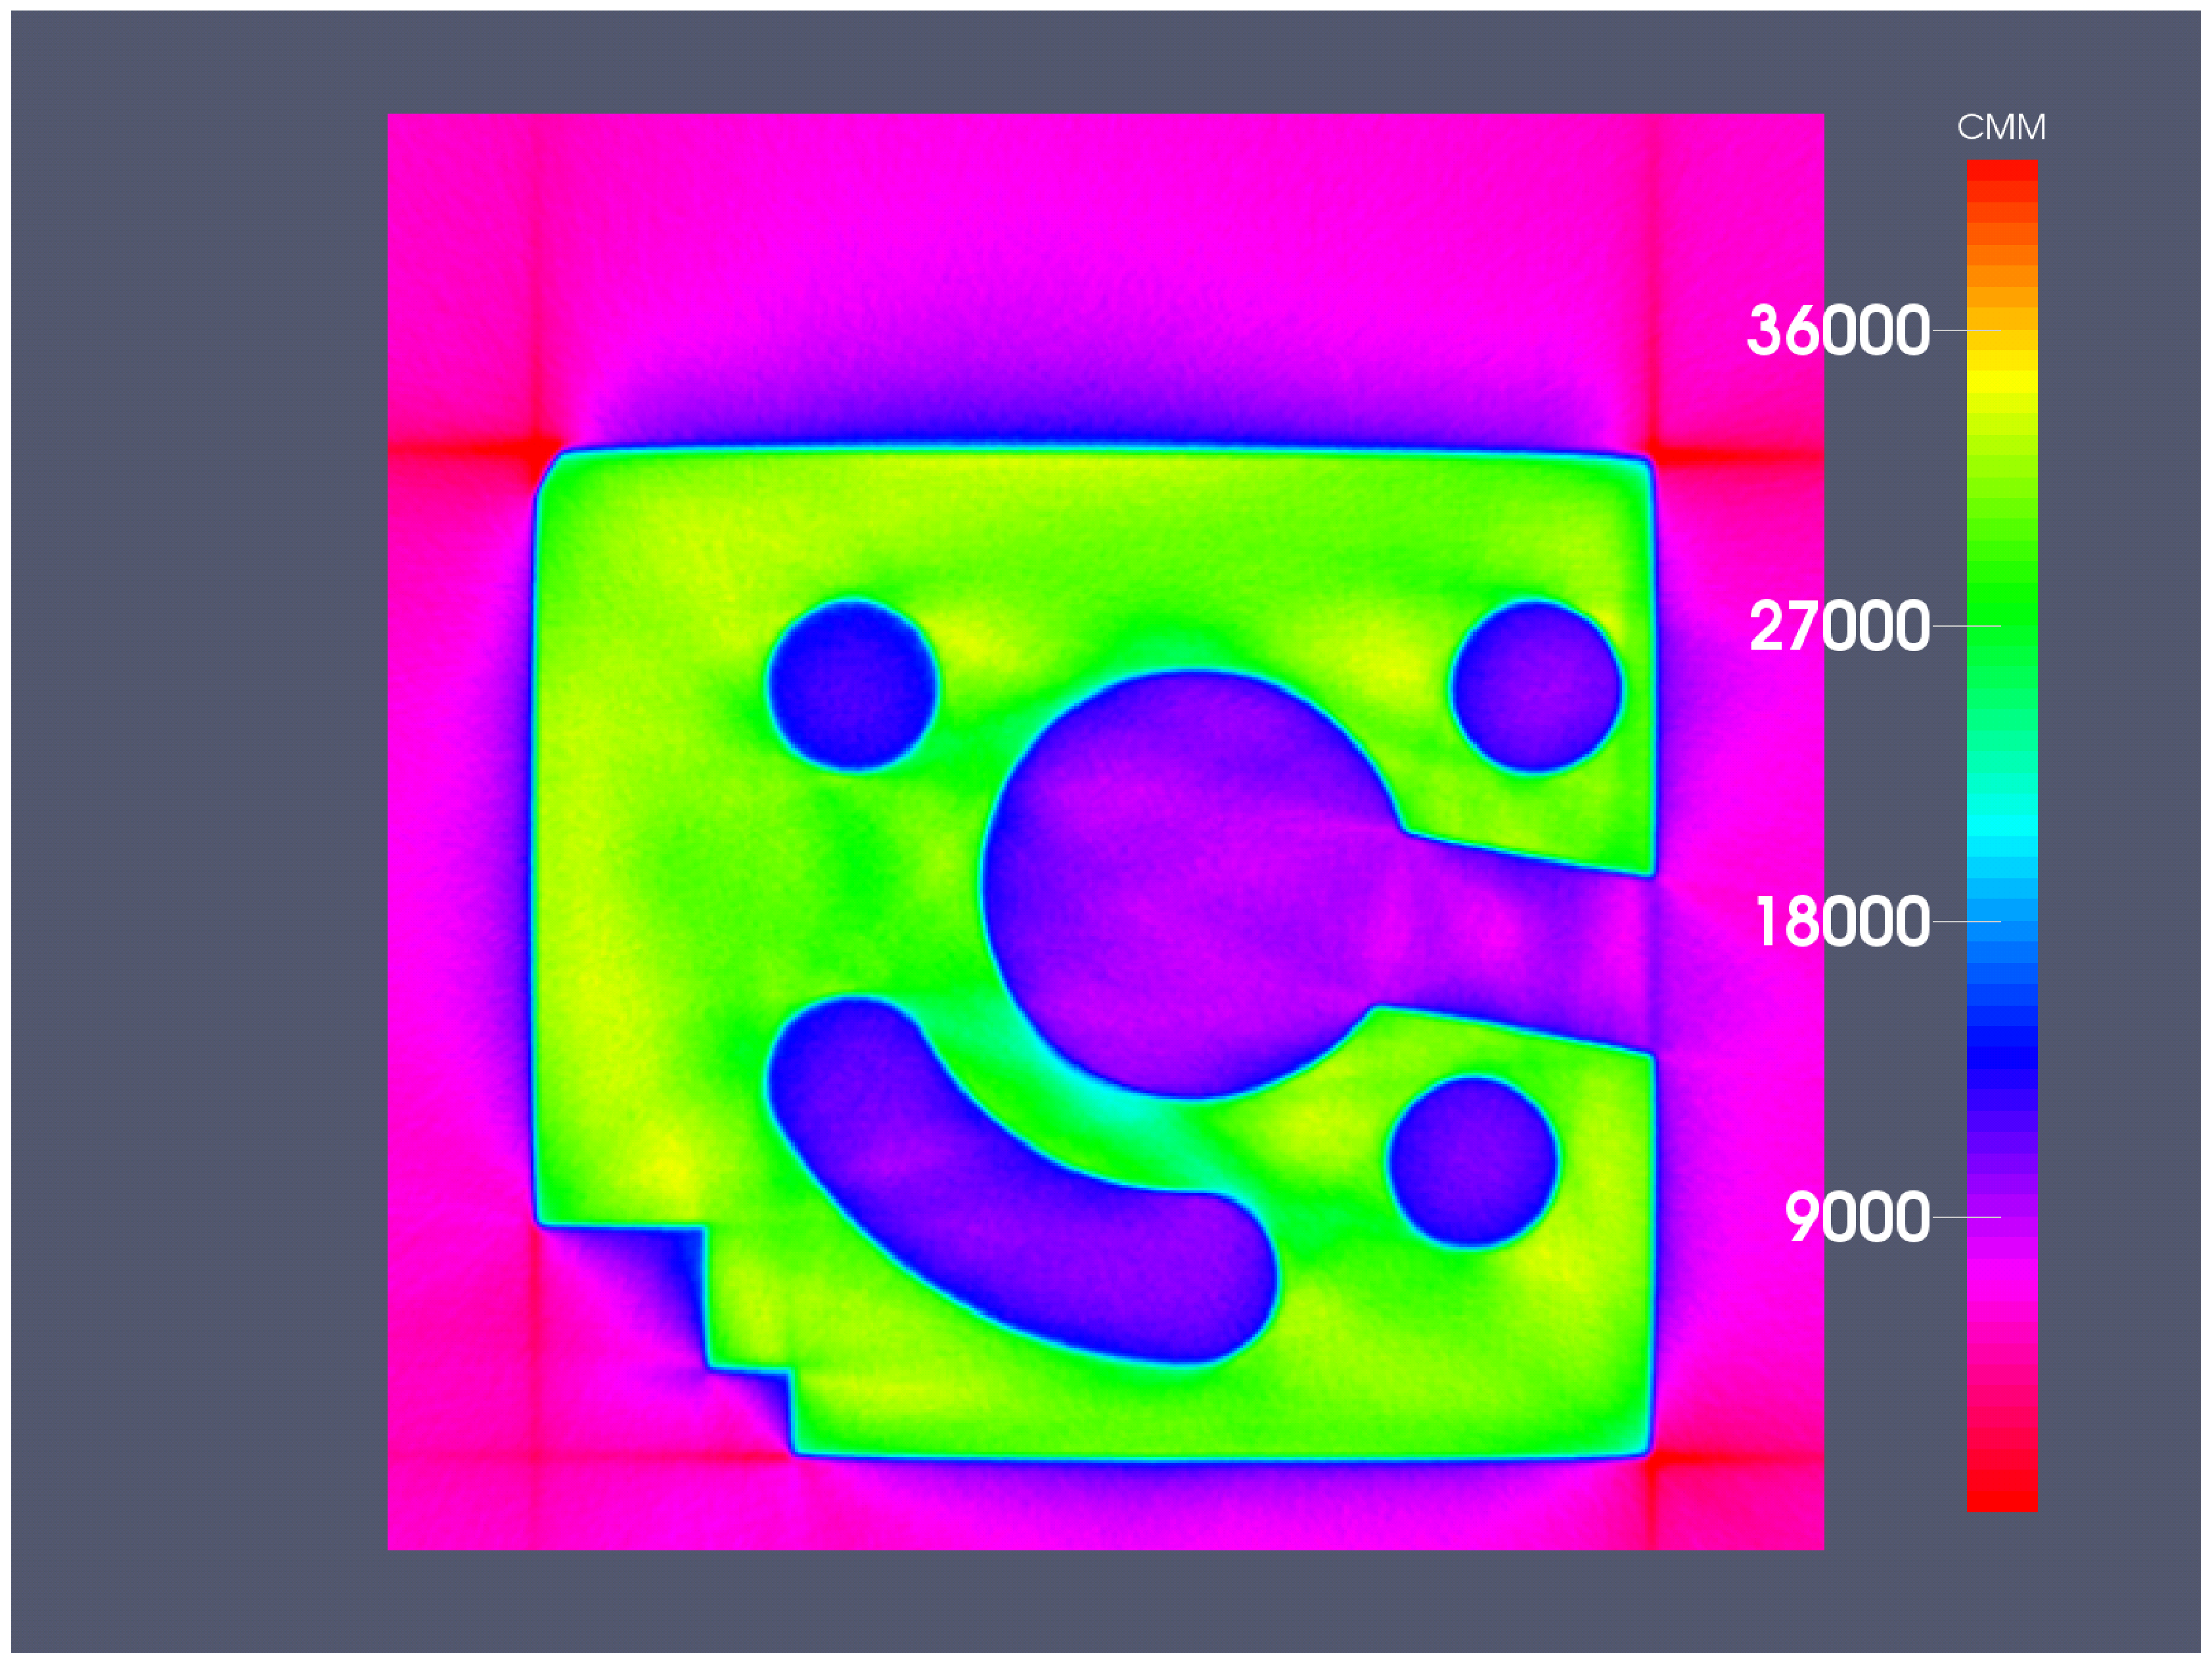
\includegraphics[width=0.3\linewidth]{images/CMM.singleSliceXY.eps}\label{fig:CMM:a}}
    \subfloat[MergeSharp Surface]{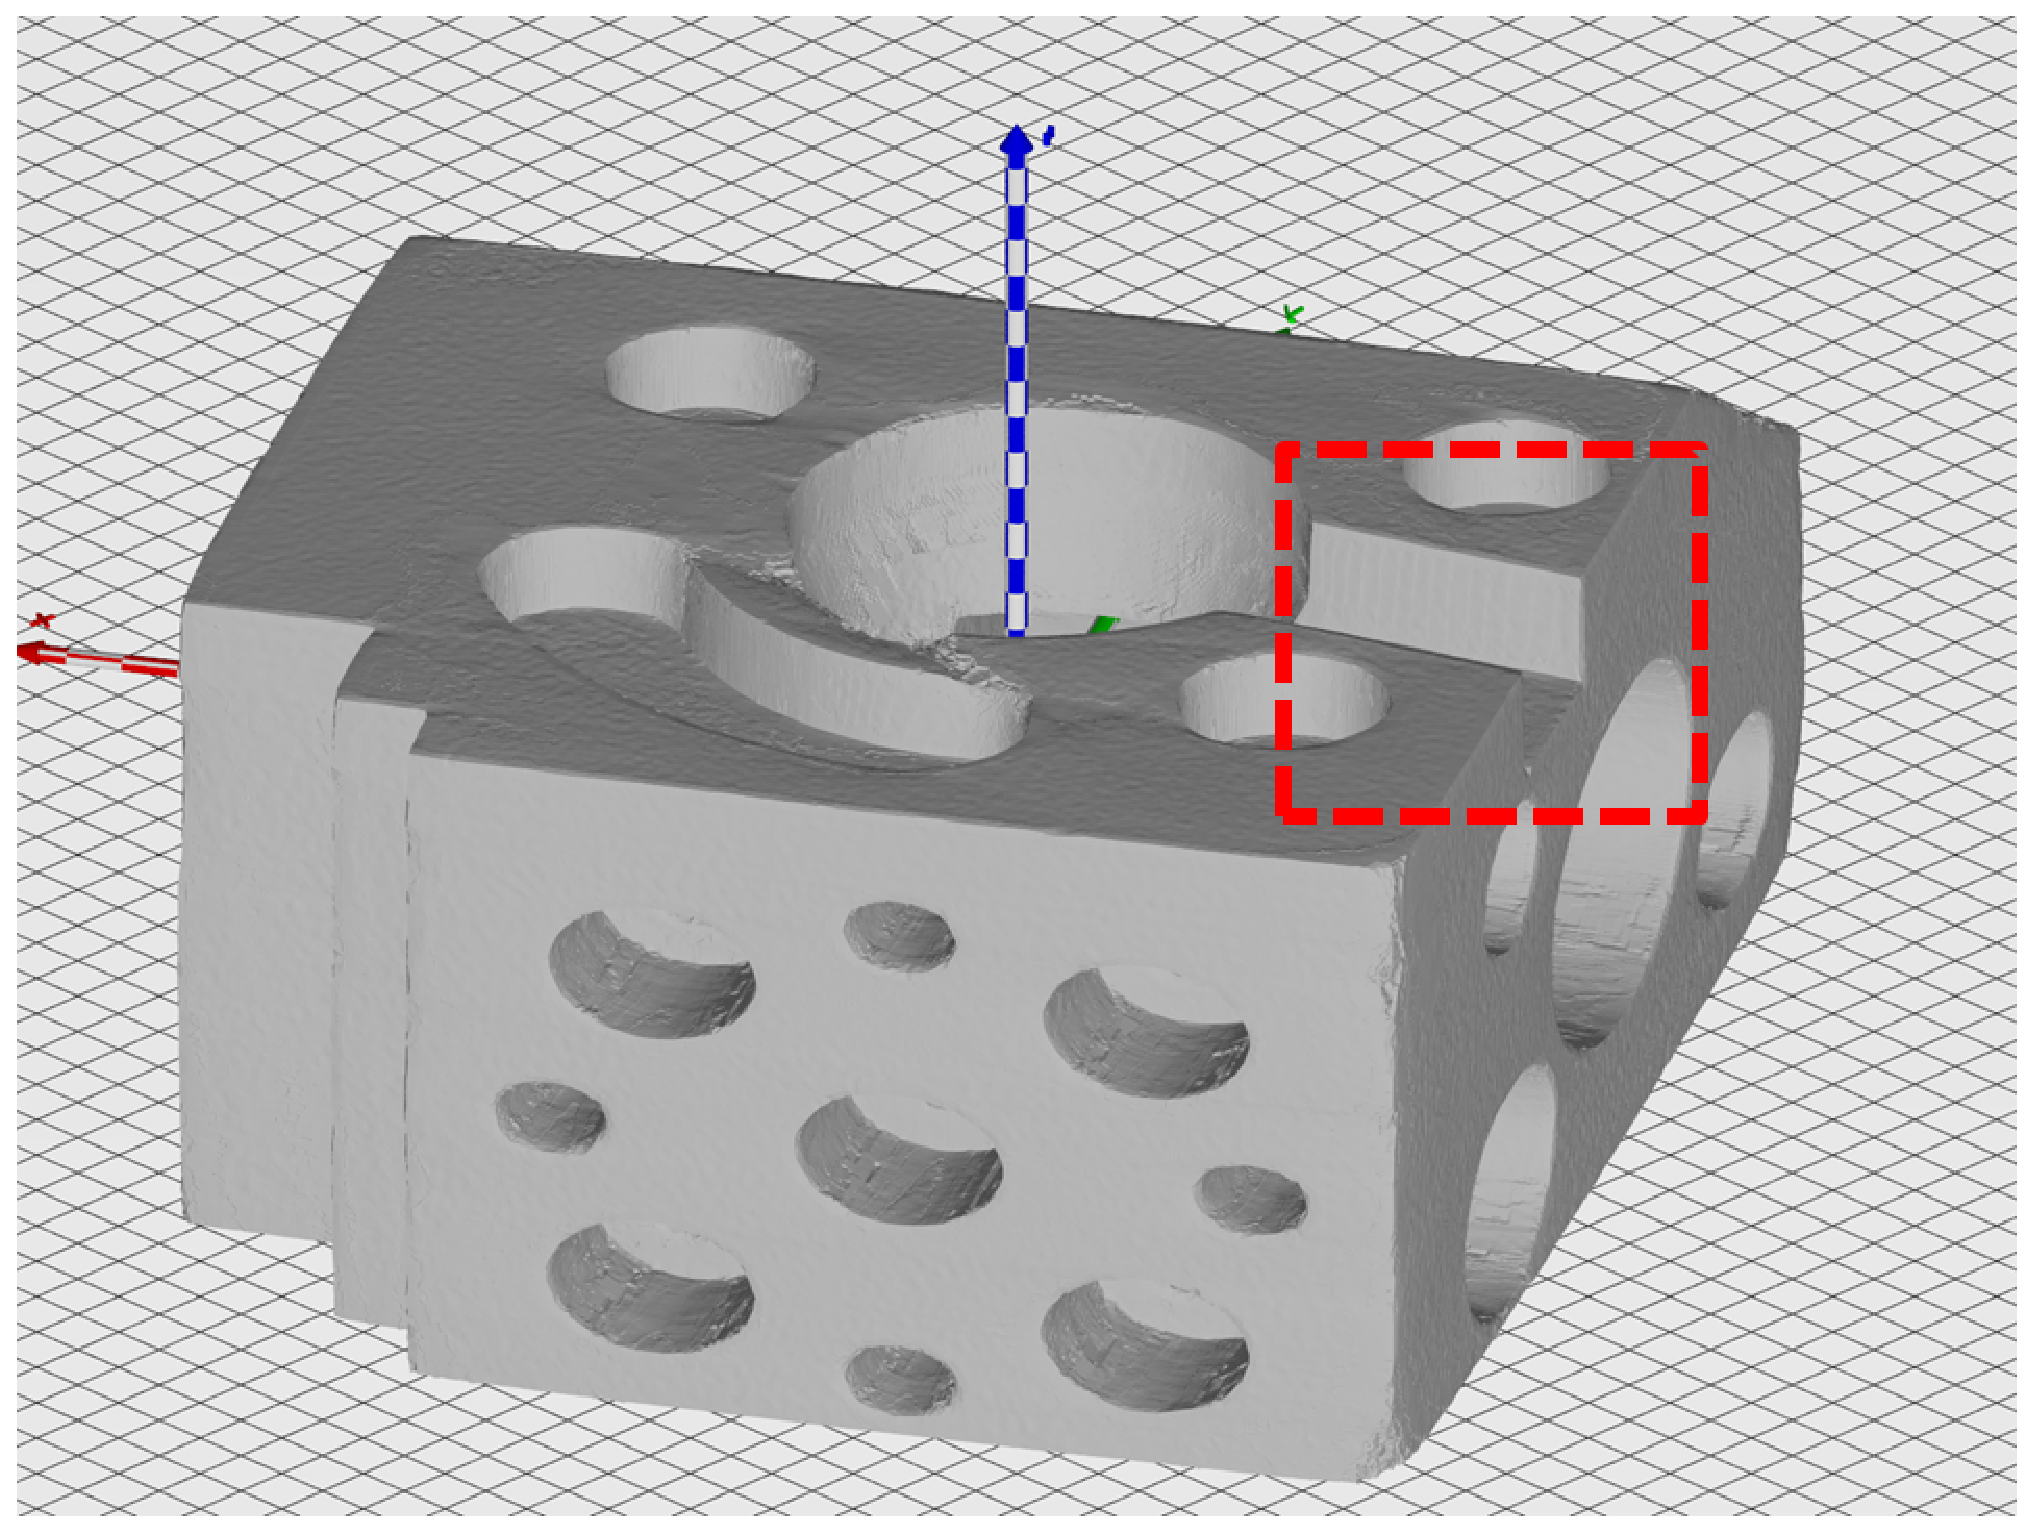
\includegraphics[width=0.3\linewidth]{images/CMM.full2.eps}\label{fig:CMM:b}}
%    \subfloat[Close Up of red square]{\includegraphics[width=0.3\linewidth]{images/CMM.close1.eps}\label{fig:CMM:c}}\hspace{1mm}
    \subfloat[Close Up of red square]{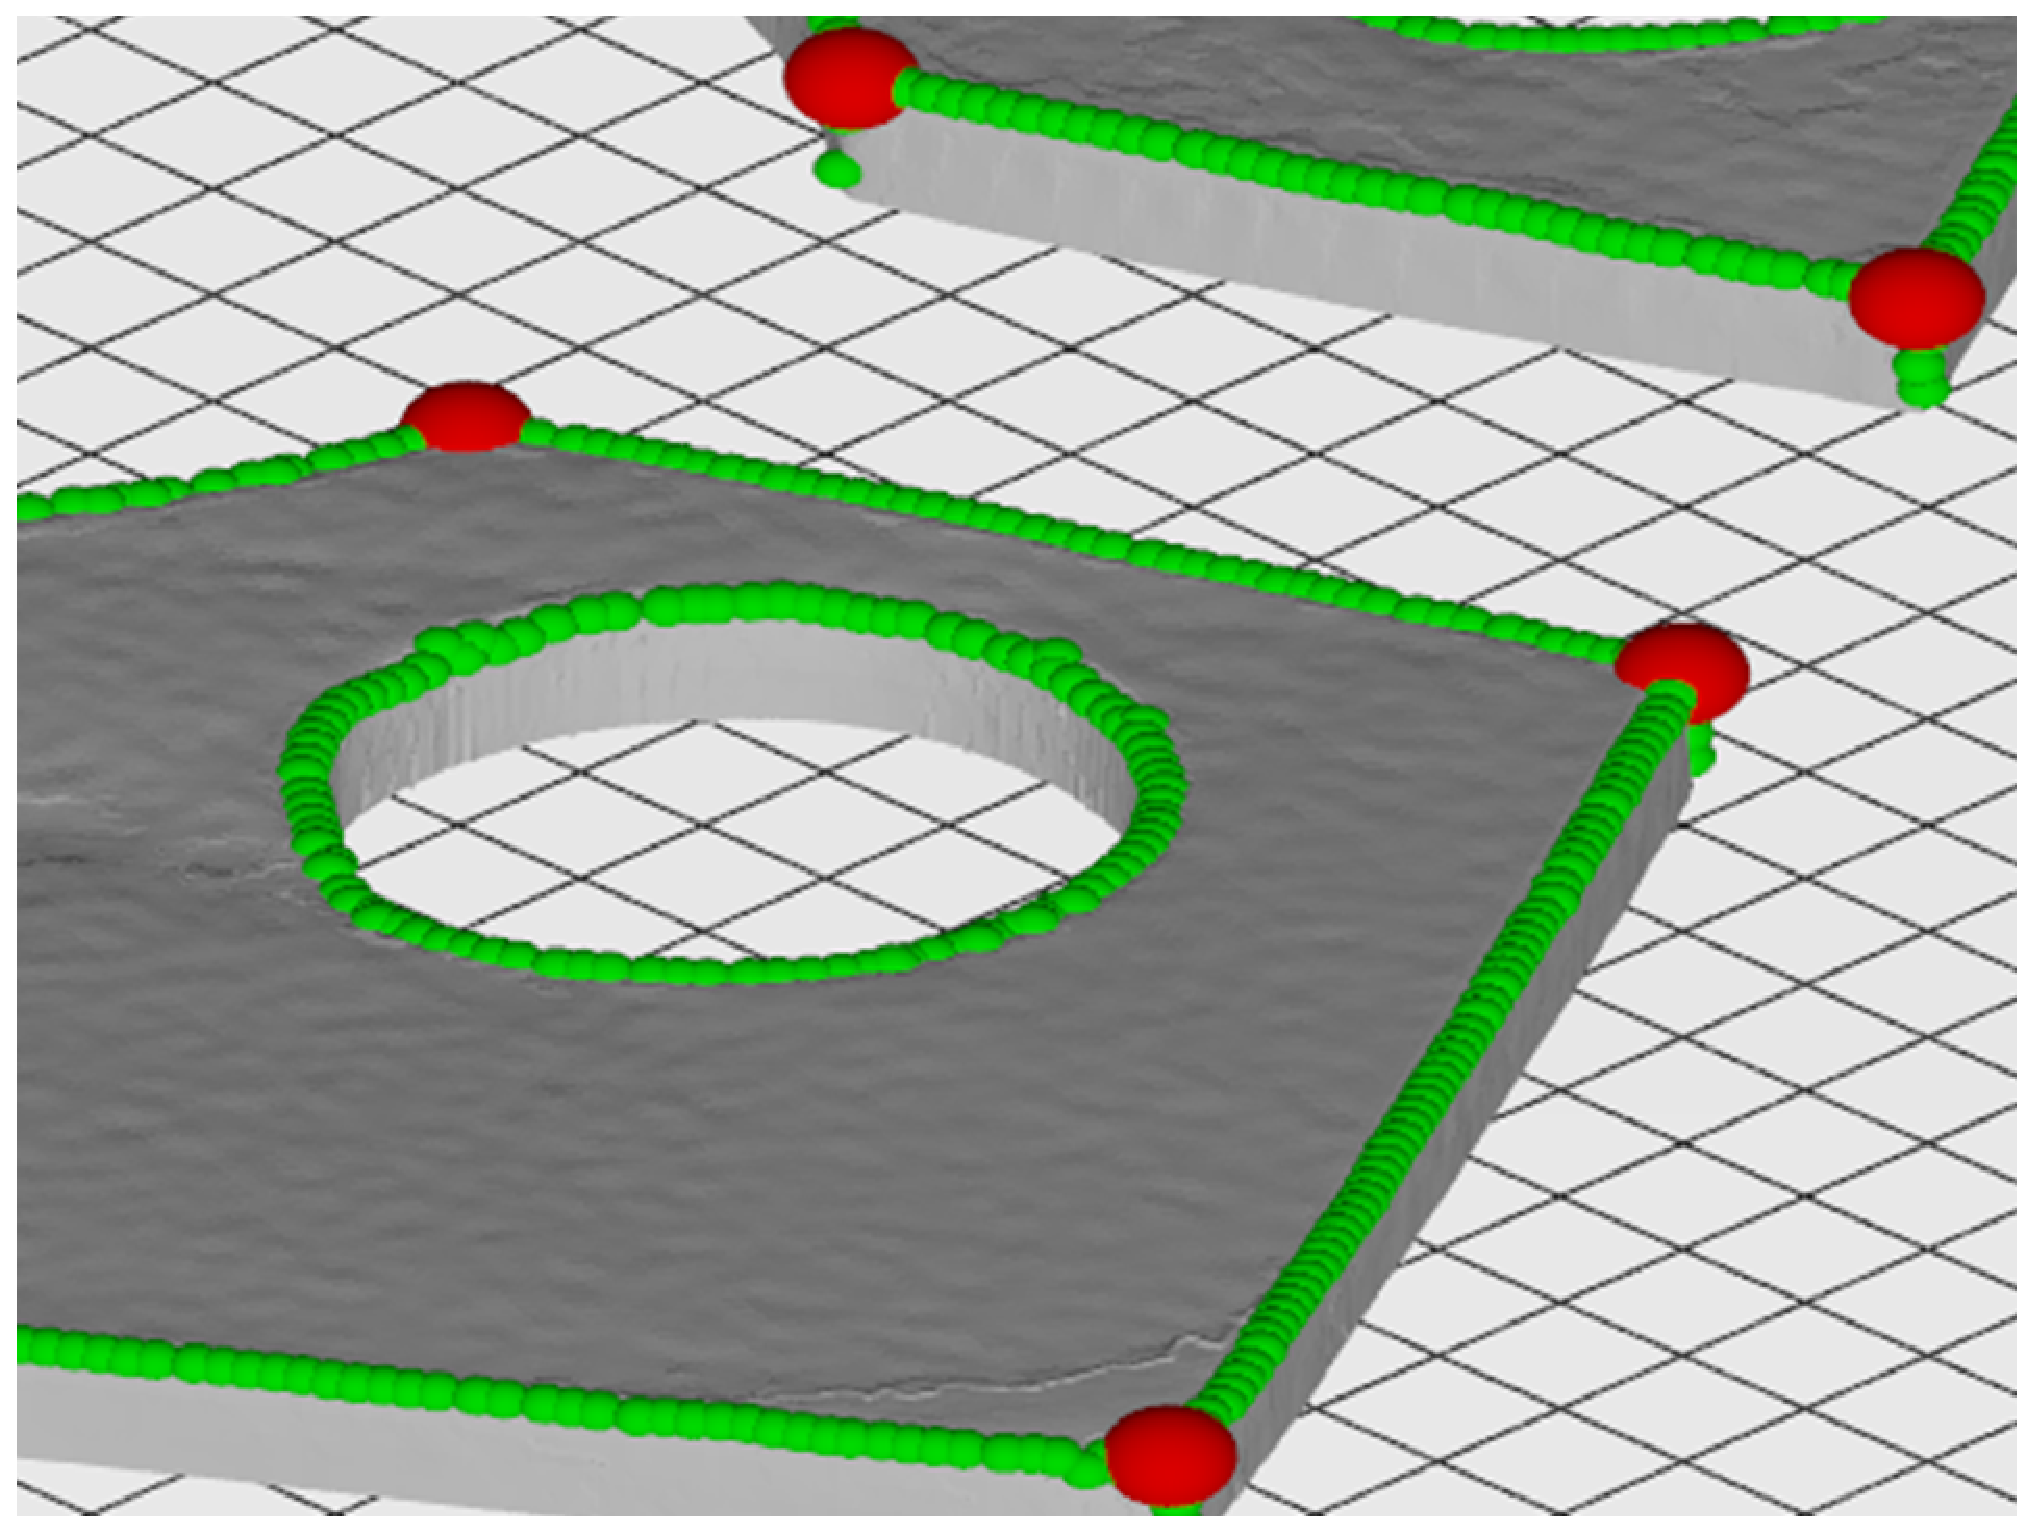
\includegraphics[width=0.3\linewidth]{images/CMM.close2.eps}\label{fig:CMM:c}}
    \caption{CMM dataset,~\protect\subref{fig:CMM:a} single slice XY plane.~\protect\subref{fig:CMM:b} MergeSharp isosurface.~\protect\subref{fig:CMM:c}  magnified red rectangle. Table~\ref{table:ictDataInfo} provides size and spacing.}
\end{figure}
\begin{figure}[htb]
    \centering
    \subfloat[Socket]{ 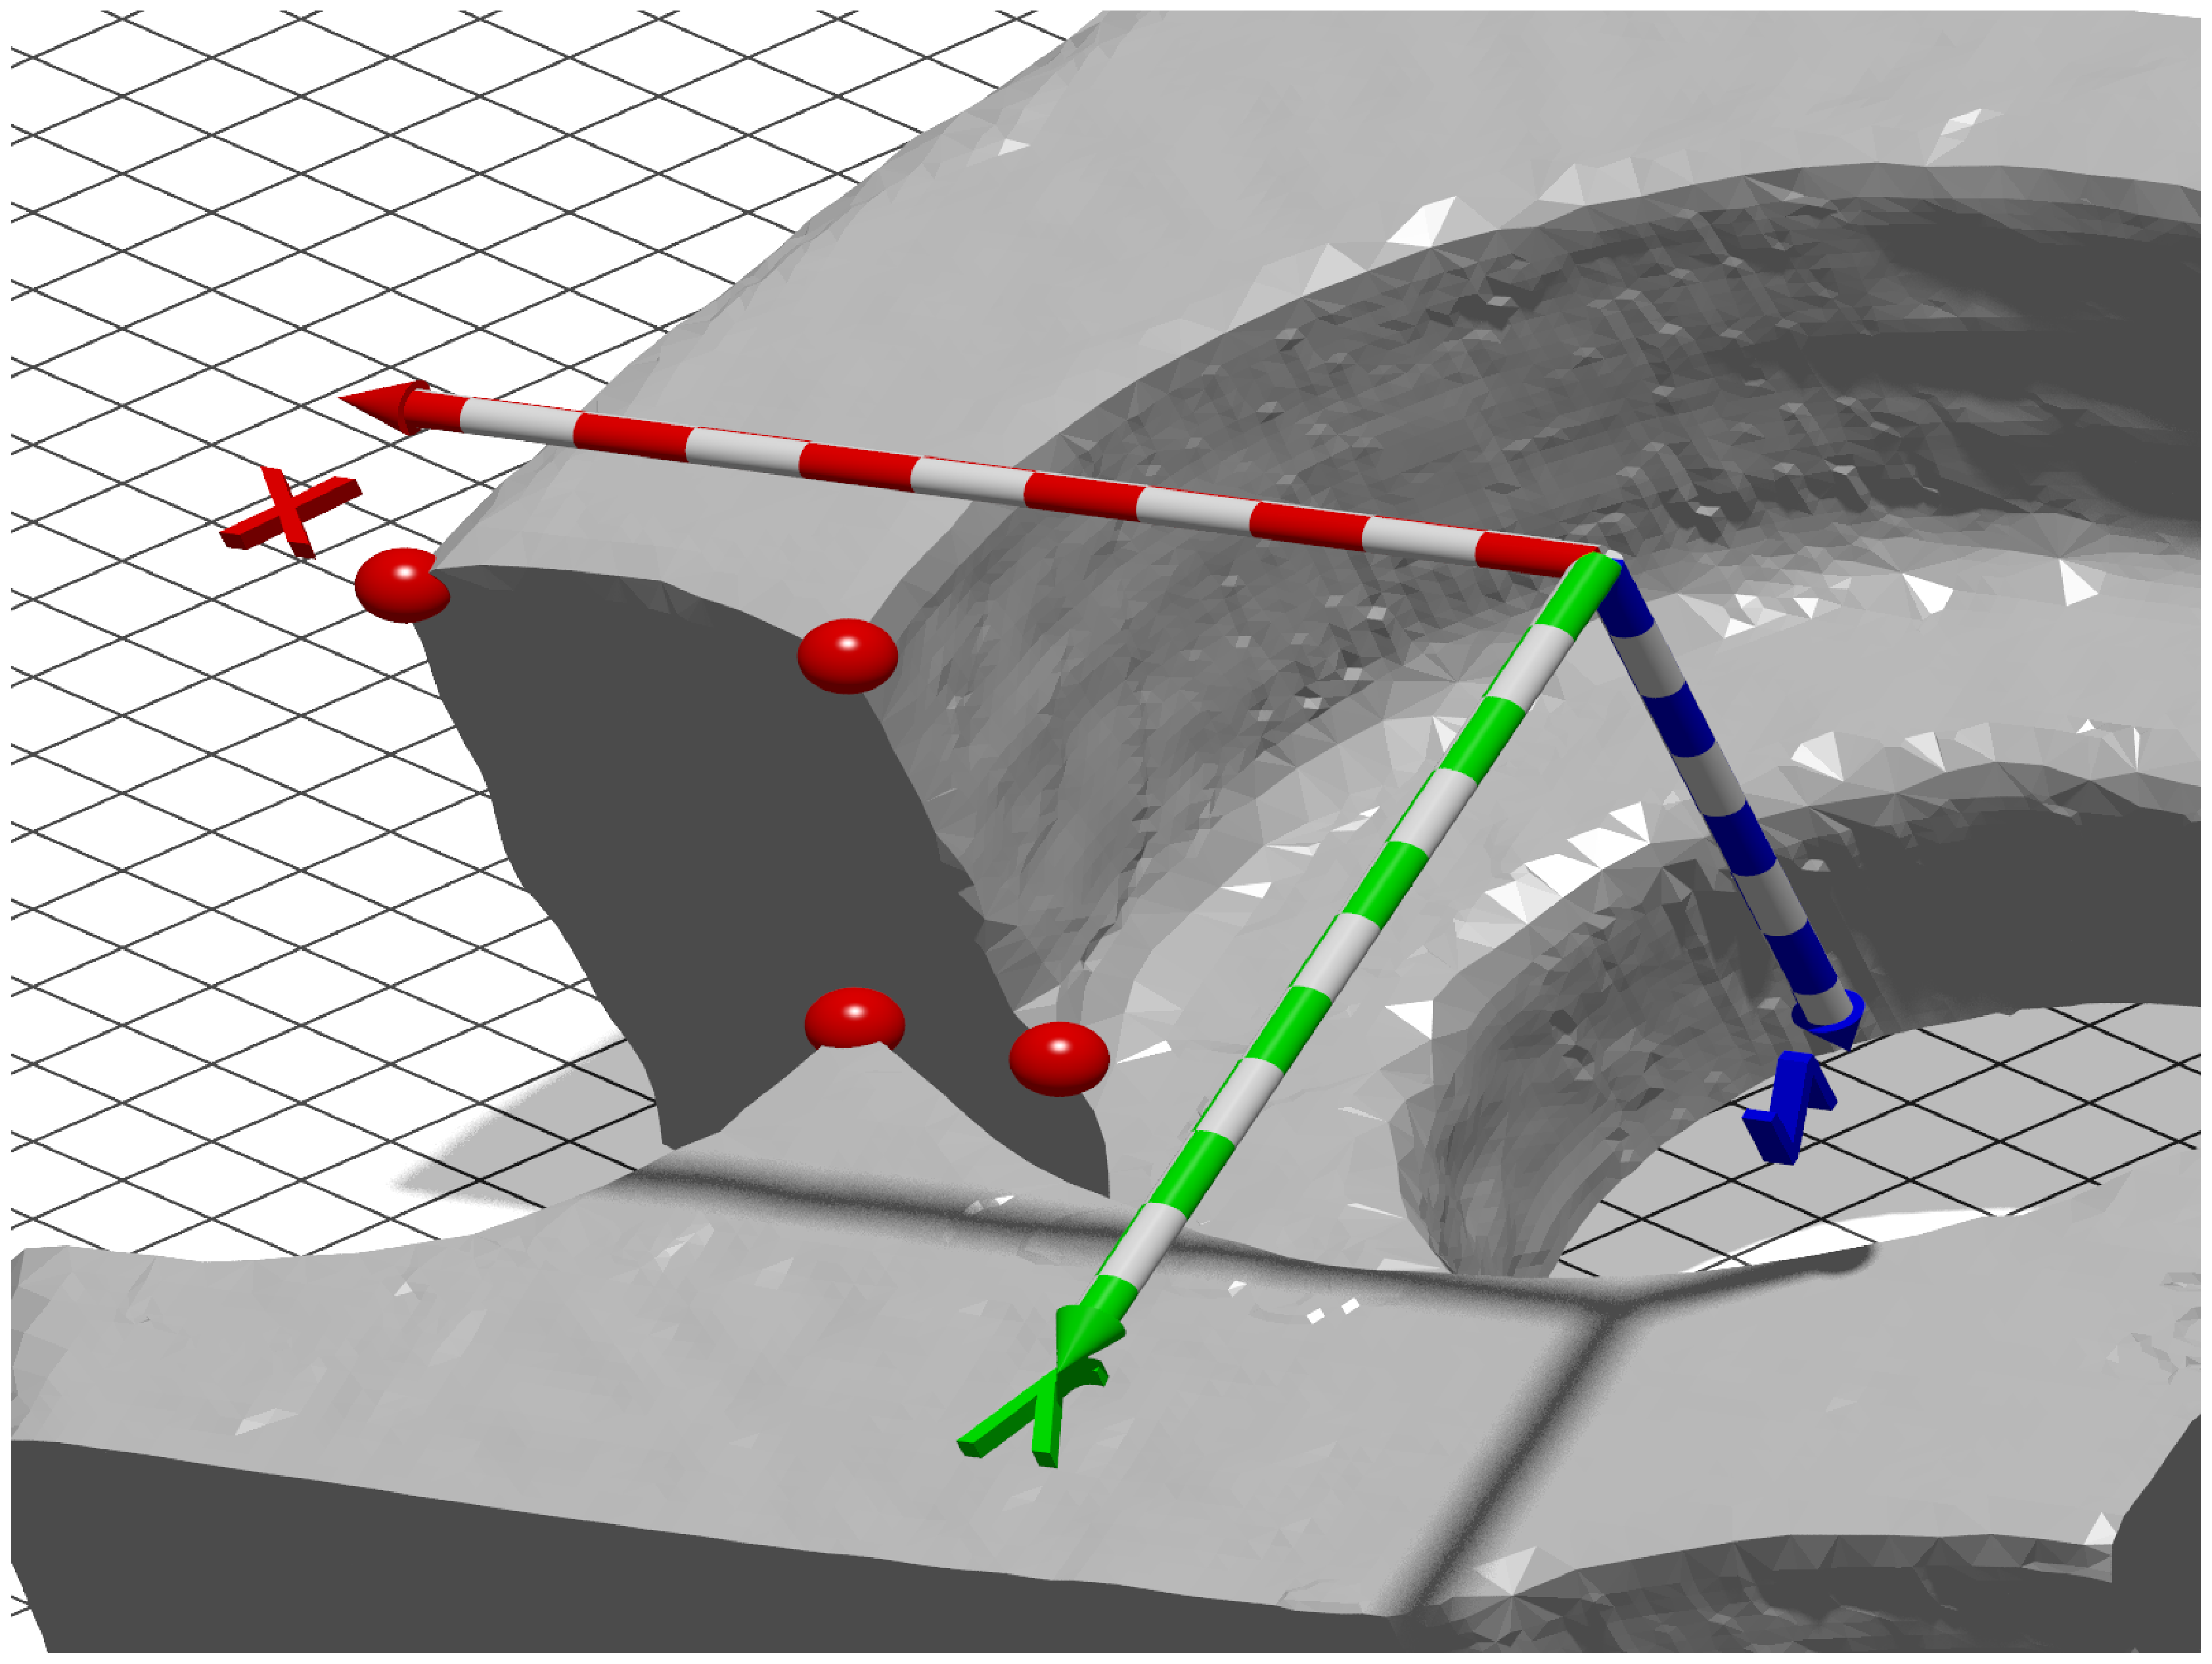
\includegraphics[width=0.3\linewidth]{images/160uCT.1a.eps}\label{fig:socket:a} }
    \subfloat[Socket Close-up]{  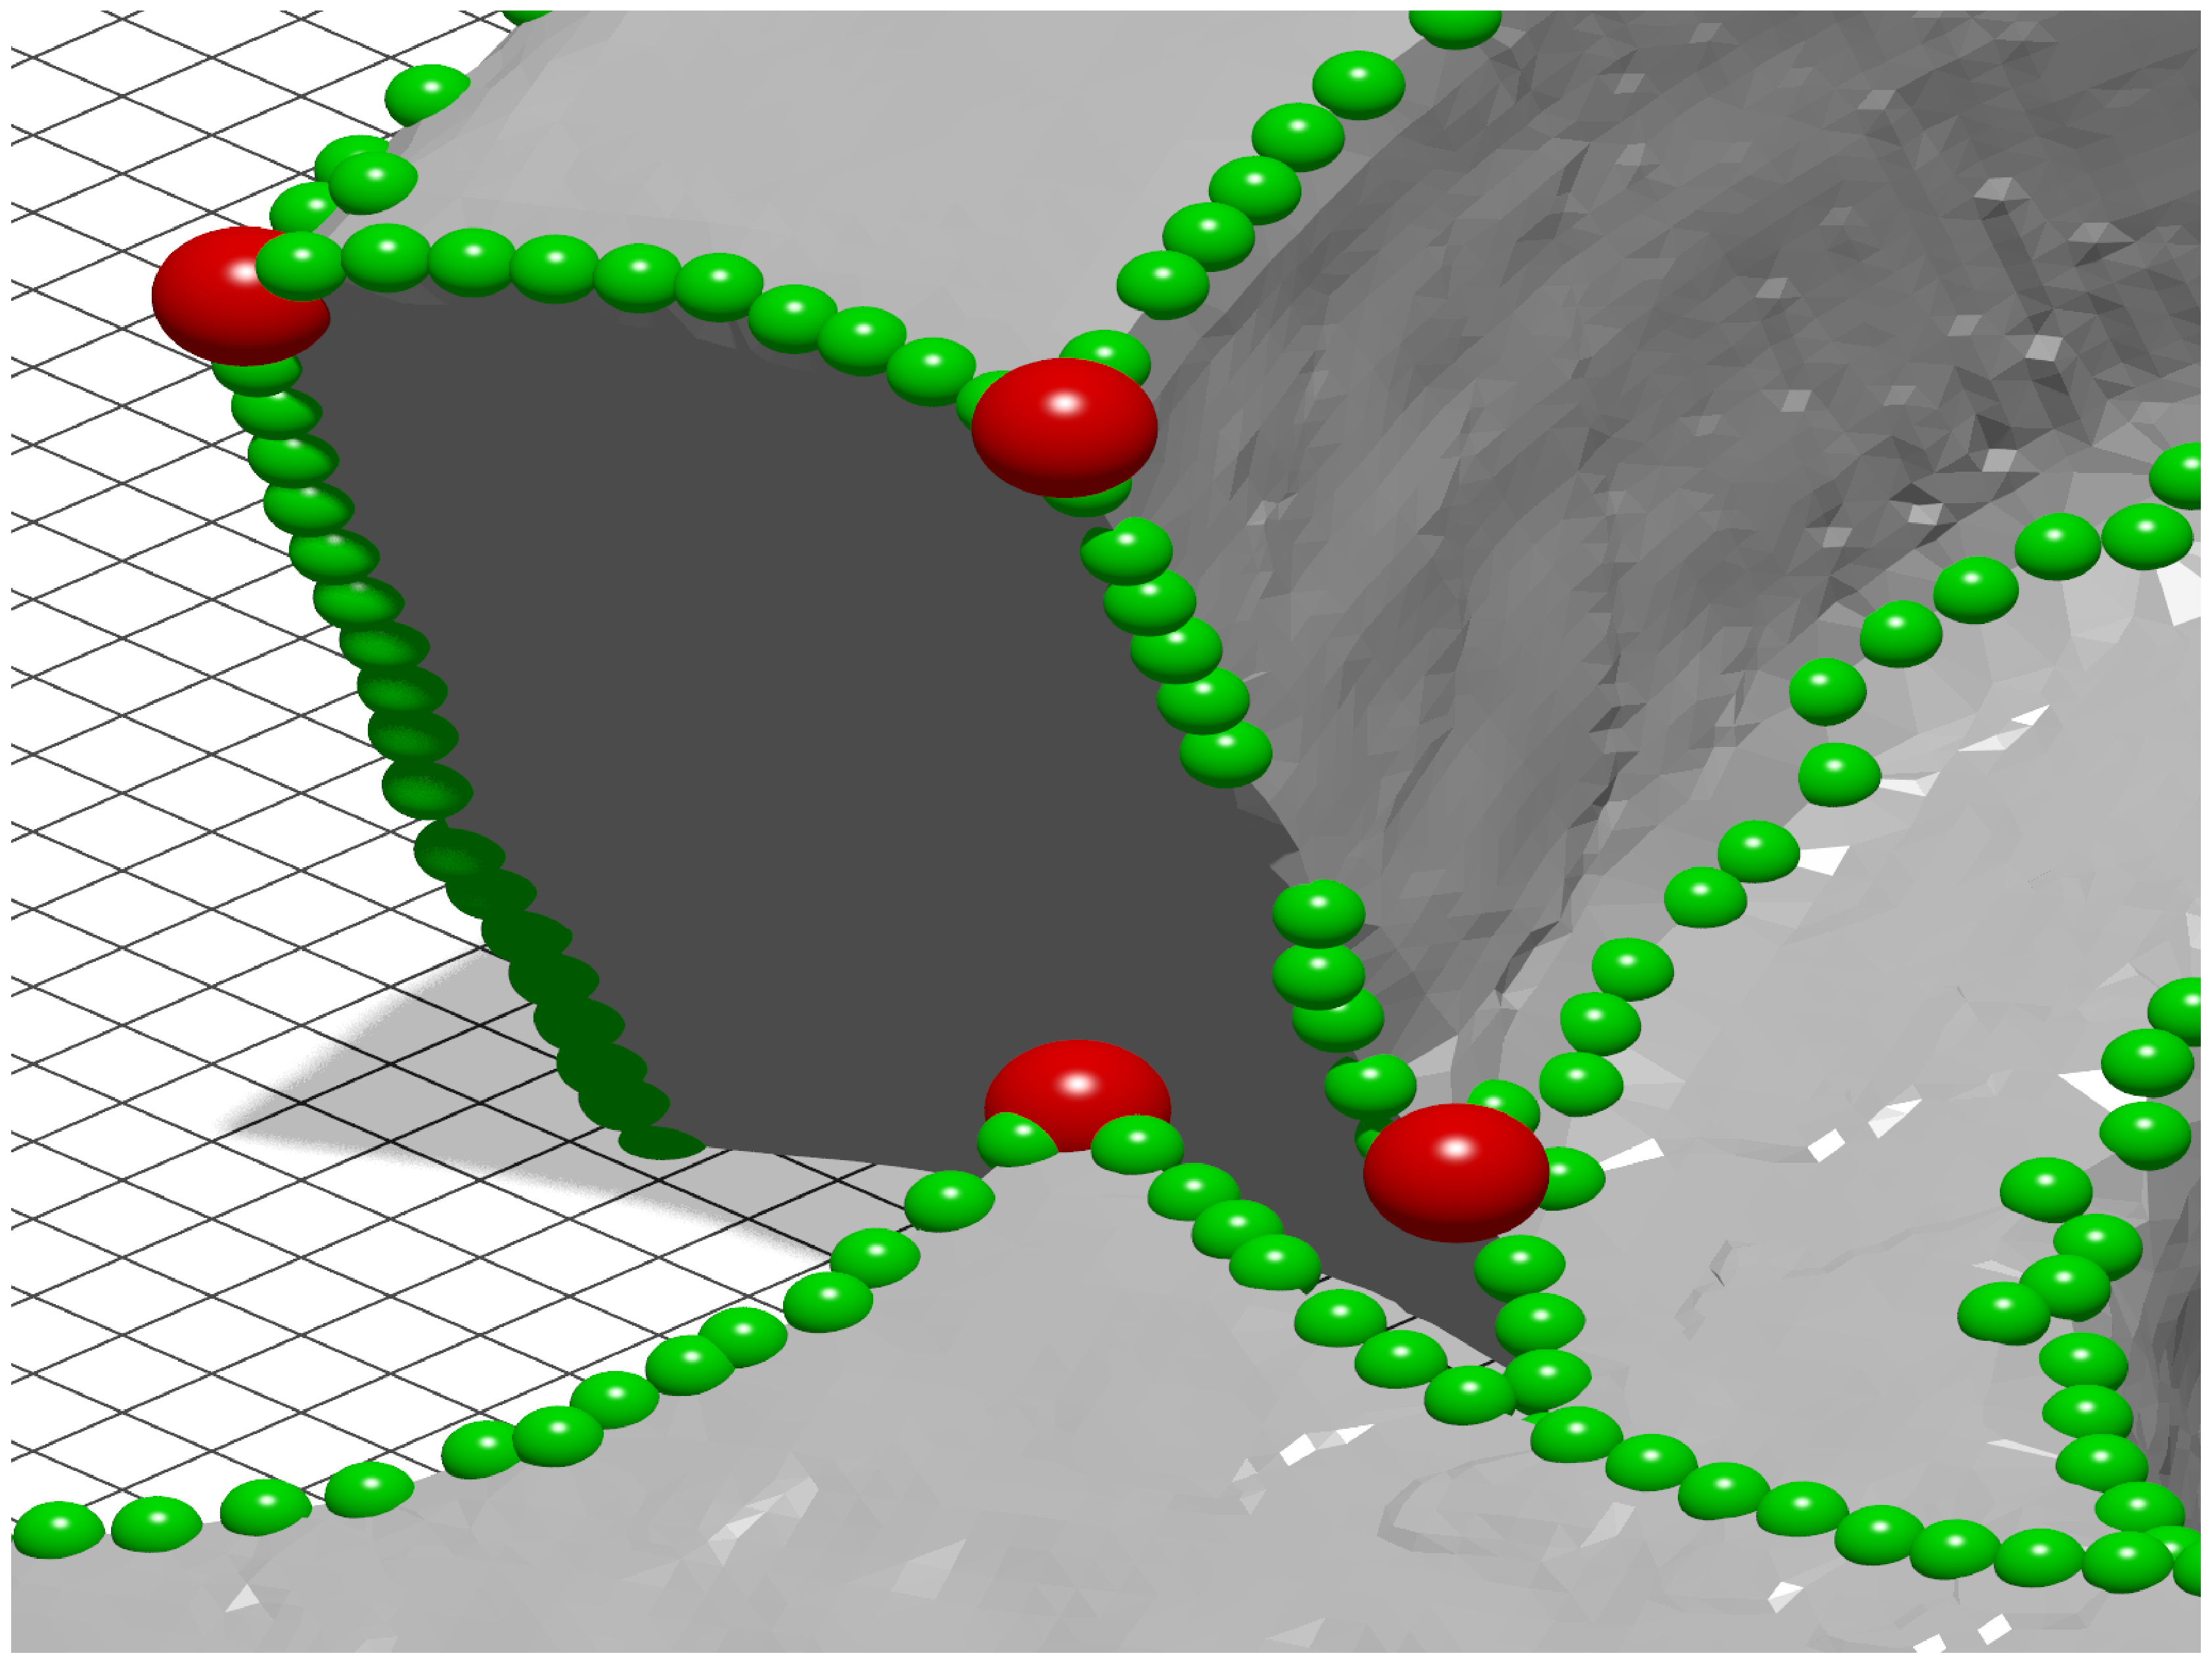
\includegraphics[width=0.3\linewidth]{images/160uCT.2.eps}\label{fig:socket:b} }   
    \subfloat[XY Slice]{  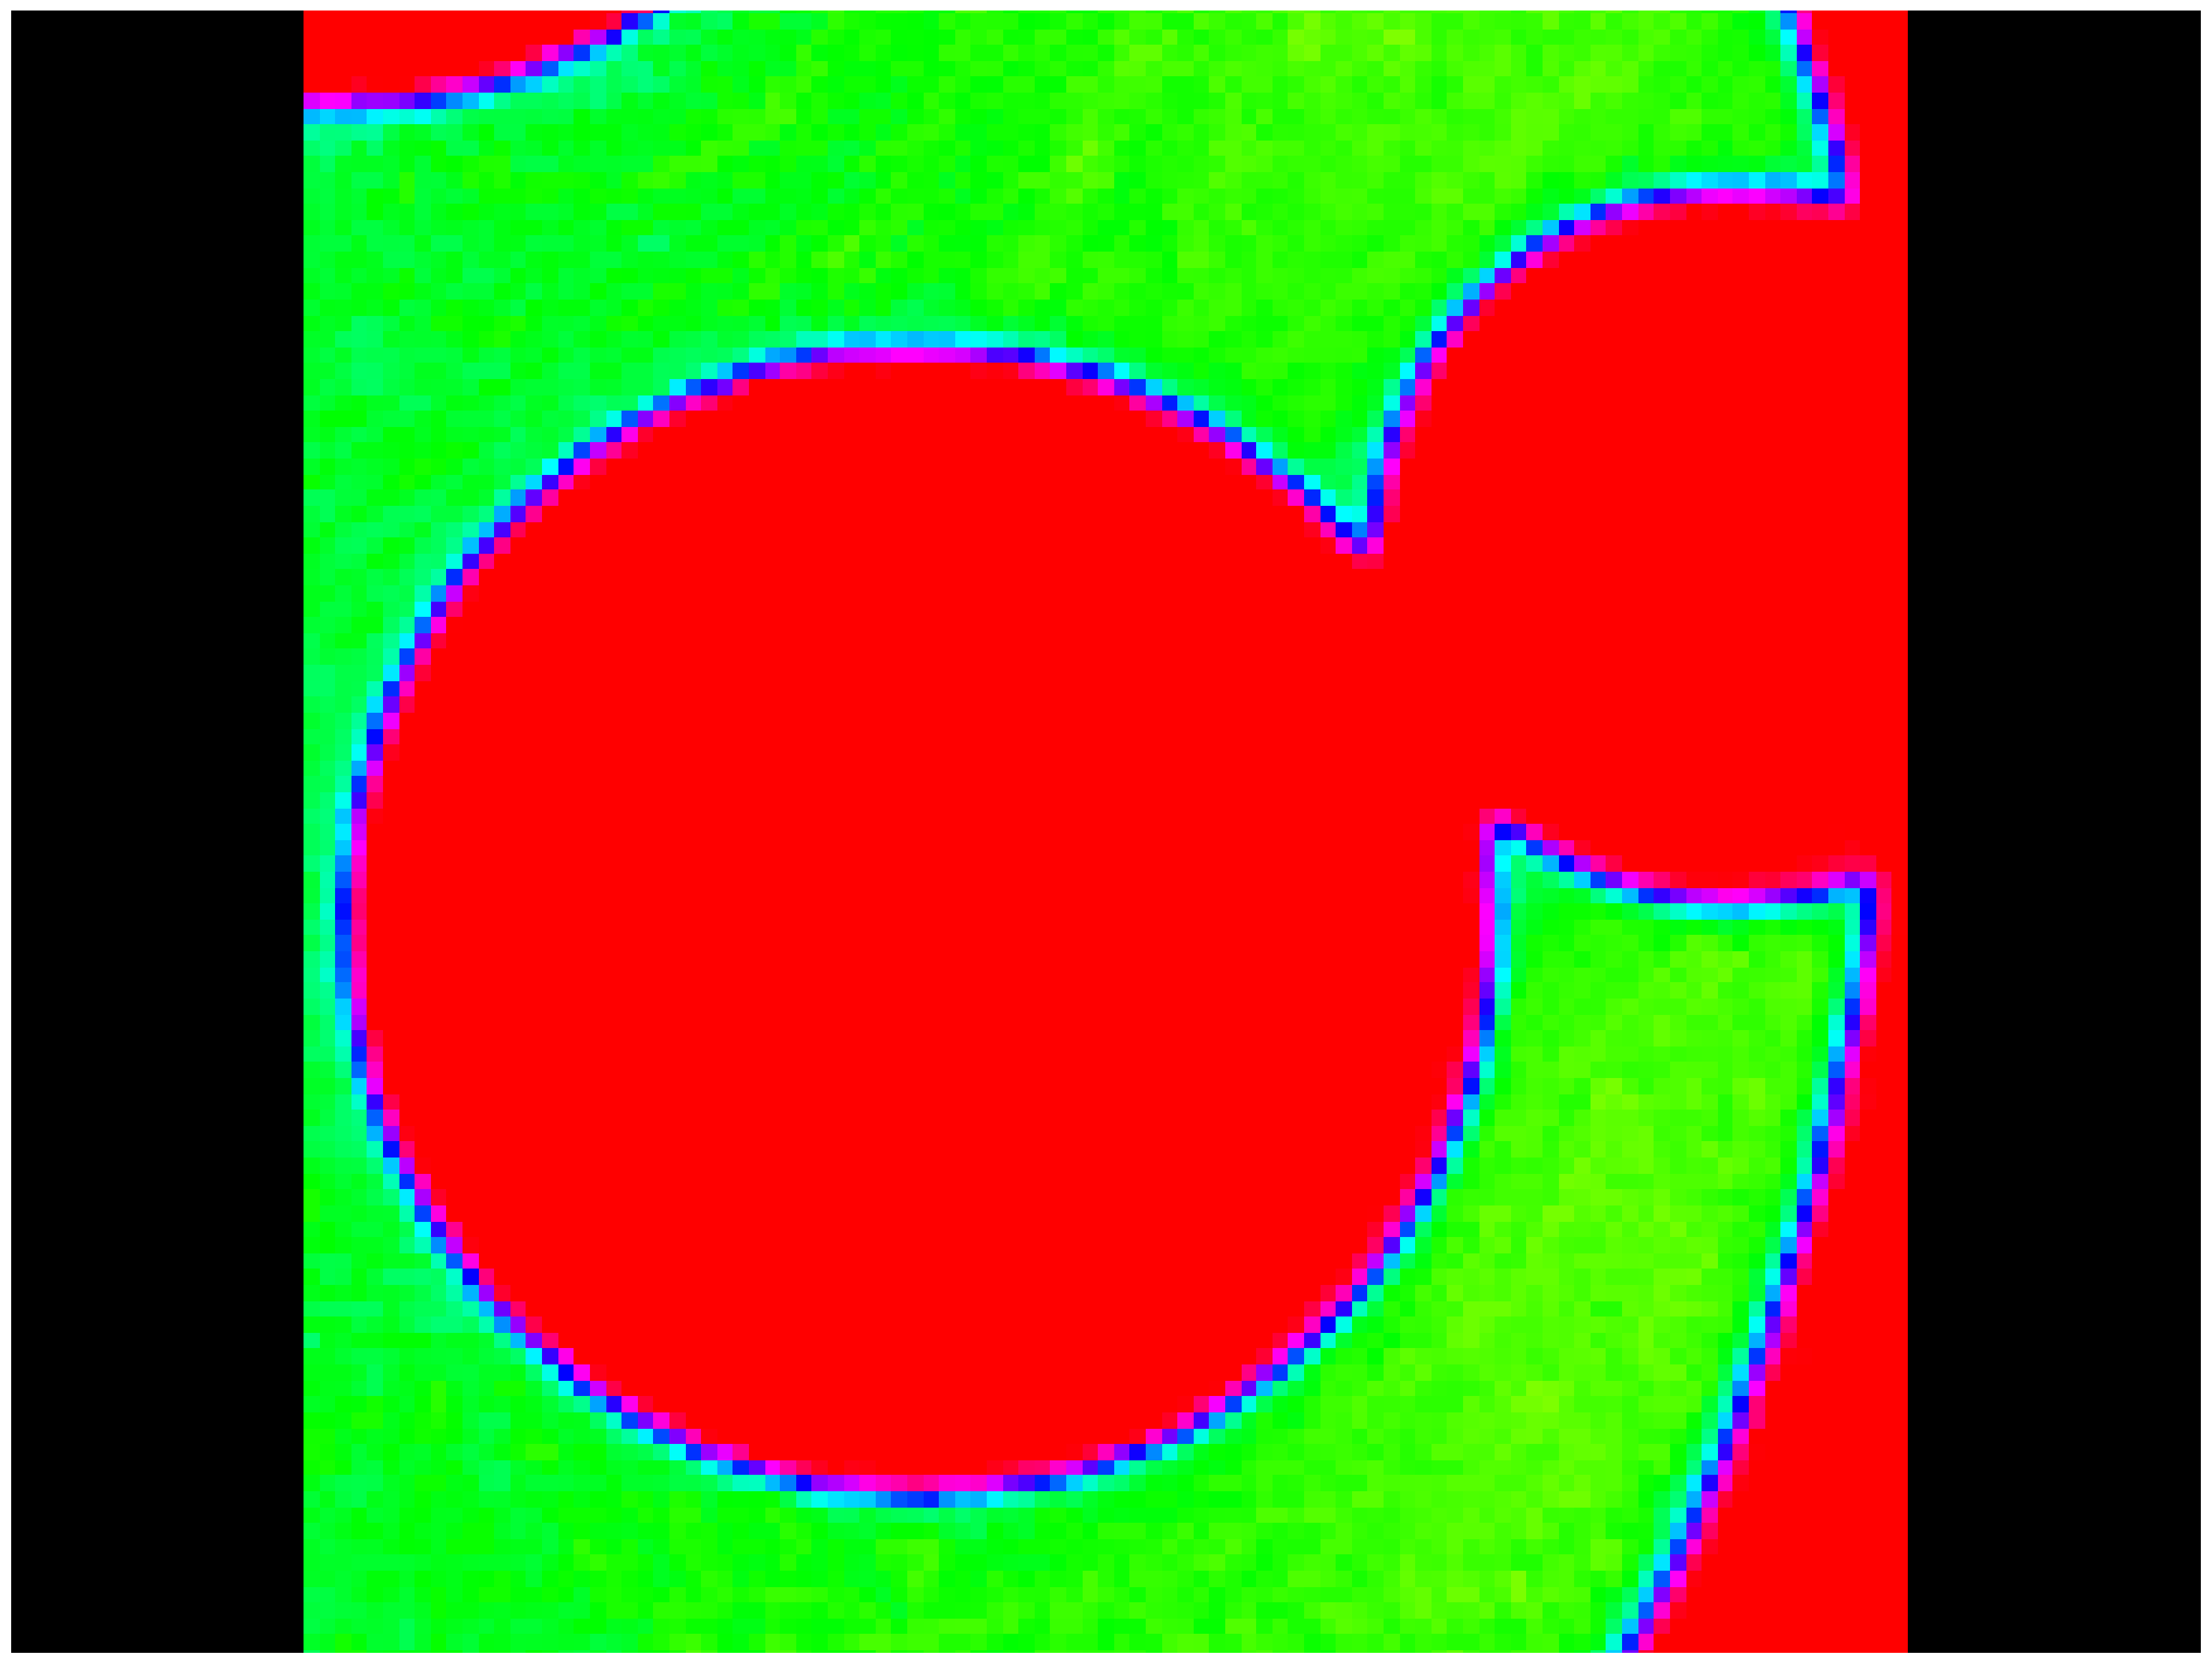
\includegraphics[width=0.3\linewidth]{images/singleSlice.eps}\label{fig:socket:c} }   
    \caption{MergeSharp mesh of a part of the socket dataset. Corners are marked in red, sparse selected edge vertices are marked in green. Figure~\ref{fig:socket:c} shows an XY slice (hsv color scale, ParaView).}
    \label{fig:socket}
\end{figure}
\subsection{Isosurface Reconstruction}
The point skeleton generated by our algorithm can be input to mesh generation algorithms
to construct an isosurface mesh.
All the meshes  in Figure~\ref{fig:SynData} are generated using \MergeSharp applied
to the sharp points from our algorithm.
Figure~\ref{fig:setA.crop1.2} shows the extracted isosurface of a part of the \emph{engine cylinder} dataset.
  Figure~\subref*{fig:CMM:b} shows the isosurface generated from the CMM data set. Figure~\subref*{fig:CMM:c} shows close up of the red rectangle in figure~\ref{fig:CMM:b}. The corner vertices are marked in red and the sparse edge vertices are marked in green. Figure~\subref*{fig:socket:a},~\subref*{fig:socket:b} shows an extracted isosurface of the socket dataset. Figure~\subref*{fig:intake:a} shows a \MergeSharp extracted mesh along with the sparse feature point skeleton of the \emph{intake} dataset.

The algorithm, WeightedCocone, by Dey et al.~\cite{dgqsww-fprss-12} constructs a surface mesh
from a point cloud which includes as input an identified set of points on sharp features.
We applied WeightedCocone on the point skeleton from the flange dataset.
We also supplied sample points on the smooth parts of the surface.
Figure~\subref*{fig:weightCocone} shows the sparse point skeleton and the resulting surface.
Other techniques which take as input feature curves/point can also
potentially use our results.

\subsection{Parameters}
Our final algorithm for CT data~\ReliGrad  has three parameters.
Among these $\alpha_{2}$ is the major parameter. $\alpha_{2}$ is a bound on the error in our prediction of a gradient at a grid vertex against the actual gradient at the vertex location. This includes, the inherent noise in the data and the change in curvature. Experimentally, we found that 10-30$^{\circ}$is a good range for this parameter. If $\alpha_{2}$ is set less than 10$^{\circ}$,
then the prediction will not be able to handle the underlying noise and change in curvature and lead to false negatives, which would mean that distance from a vertex with unreliable gradient to one with reliable gradient will be large.
While,$\alpha_{2}$ to be greater than 30$^{\circ}$ would mean more false positives, and erroneous gradients might be  marked reliable. 

\begin{table}[h]
    \begin{tabular}{|l|l|l|l|l|}
        \hline
        \multirow{2}{*}{\begin{tabular}[c]{@{}l@{}}$\alpha_{2}$\\ in $^{\circ}$\end{tabular}} & \multicolumn{2}{l|}{Flange}                                                                                                & \multicolumn{2}{l|}{TwoCube}                                                    \\ \cline{2-5} 
        & \begin{tabular}[c]{@{}l@{}}MaxAngleDiff\\ in $^\circ$s\end{tabular} & \begin{tabular}[c]{@{}l@{}}Dist\\ 2Grad\end{tabular} & MaxAngleDiffin $^\circ$s & \begin{tabular}[c]{@{}l@{}}Dist\\ 2Grad\end{tabular} \\ \hline
        5                                                                                     & 4.11                                                                & 5                                                    & 3.3                      & 5                                                    \\ \hline
        10                                                                                    & 9.8                                                                 & 5                                                    & 8.0                      & 5                                                    \\ \hline
        15                                                                                    & 14.2                                                                & 4                                                    & 14.4                     & 4                                                    \\ \hline
        20                                                                                    & 19.7                                                                & 4                                                    & 19.2                     & 3                                                    \\ \hline
        25                                                                                    & 21.9*                                                               & 4                                                    & 37.3*                    & 3                                                    \\ \hline
        30                                                                                    & 25.0*                                                               & 4                                                    & 73.1*                    & 3                                                    \\ \hline
    \end{tabular}
    \caption{Effect of changing parameter $\alpha_{2}$ in \protect\ReliGrad.}
    \label{table:parameter}
\end{table}
Table~\ref{table:parameter} shows the effect of changing $\alpha_{2}$ on maxAngleDiff and Dist2Grad on the \textit{flange} and \textit{TwoCube} dataset. As expected, the maximum angle difference to the known correct gradients increases with increasing $\alpha_{2}$. While the maximum angle is 73.1 degrees, for \textit{TwoCube} with $\alpha_{2}$ set to 30 degrees, there were only 2 vertices with angle greater than 30 degrees. The \MergeSharp reconstruction showed no visible errors. 
 $\alpha_{1}$ decides if gradients at two vertices agree with each other. This is a much tighter threshold. For all our experiments this was set to 5$^{\circ}$s. We also always fixed the numIter, which decides how many times the reliable gradients are extended to 2, for all our tests. 
  
\begin{figure}
    \centering
    \subfloat[intake valve]{ 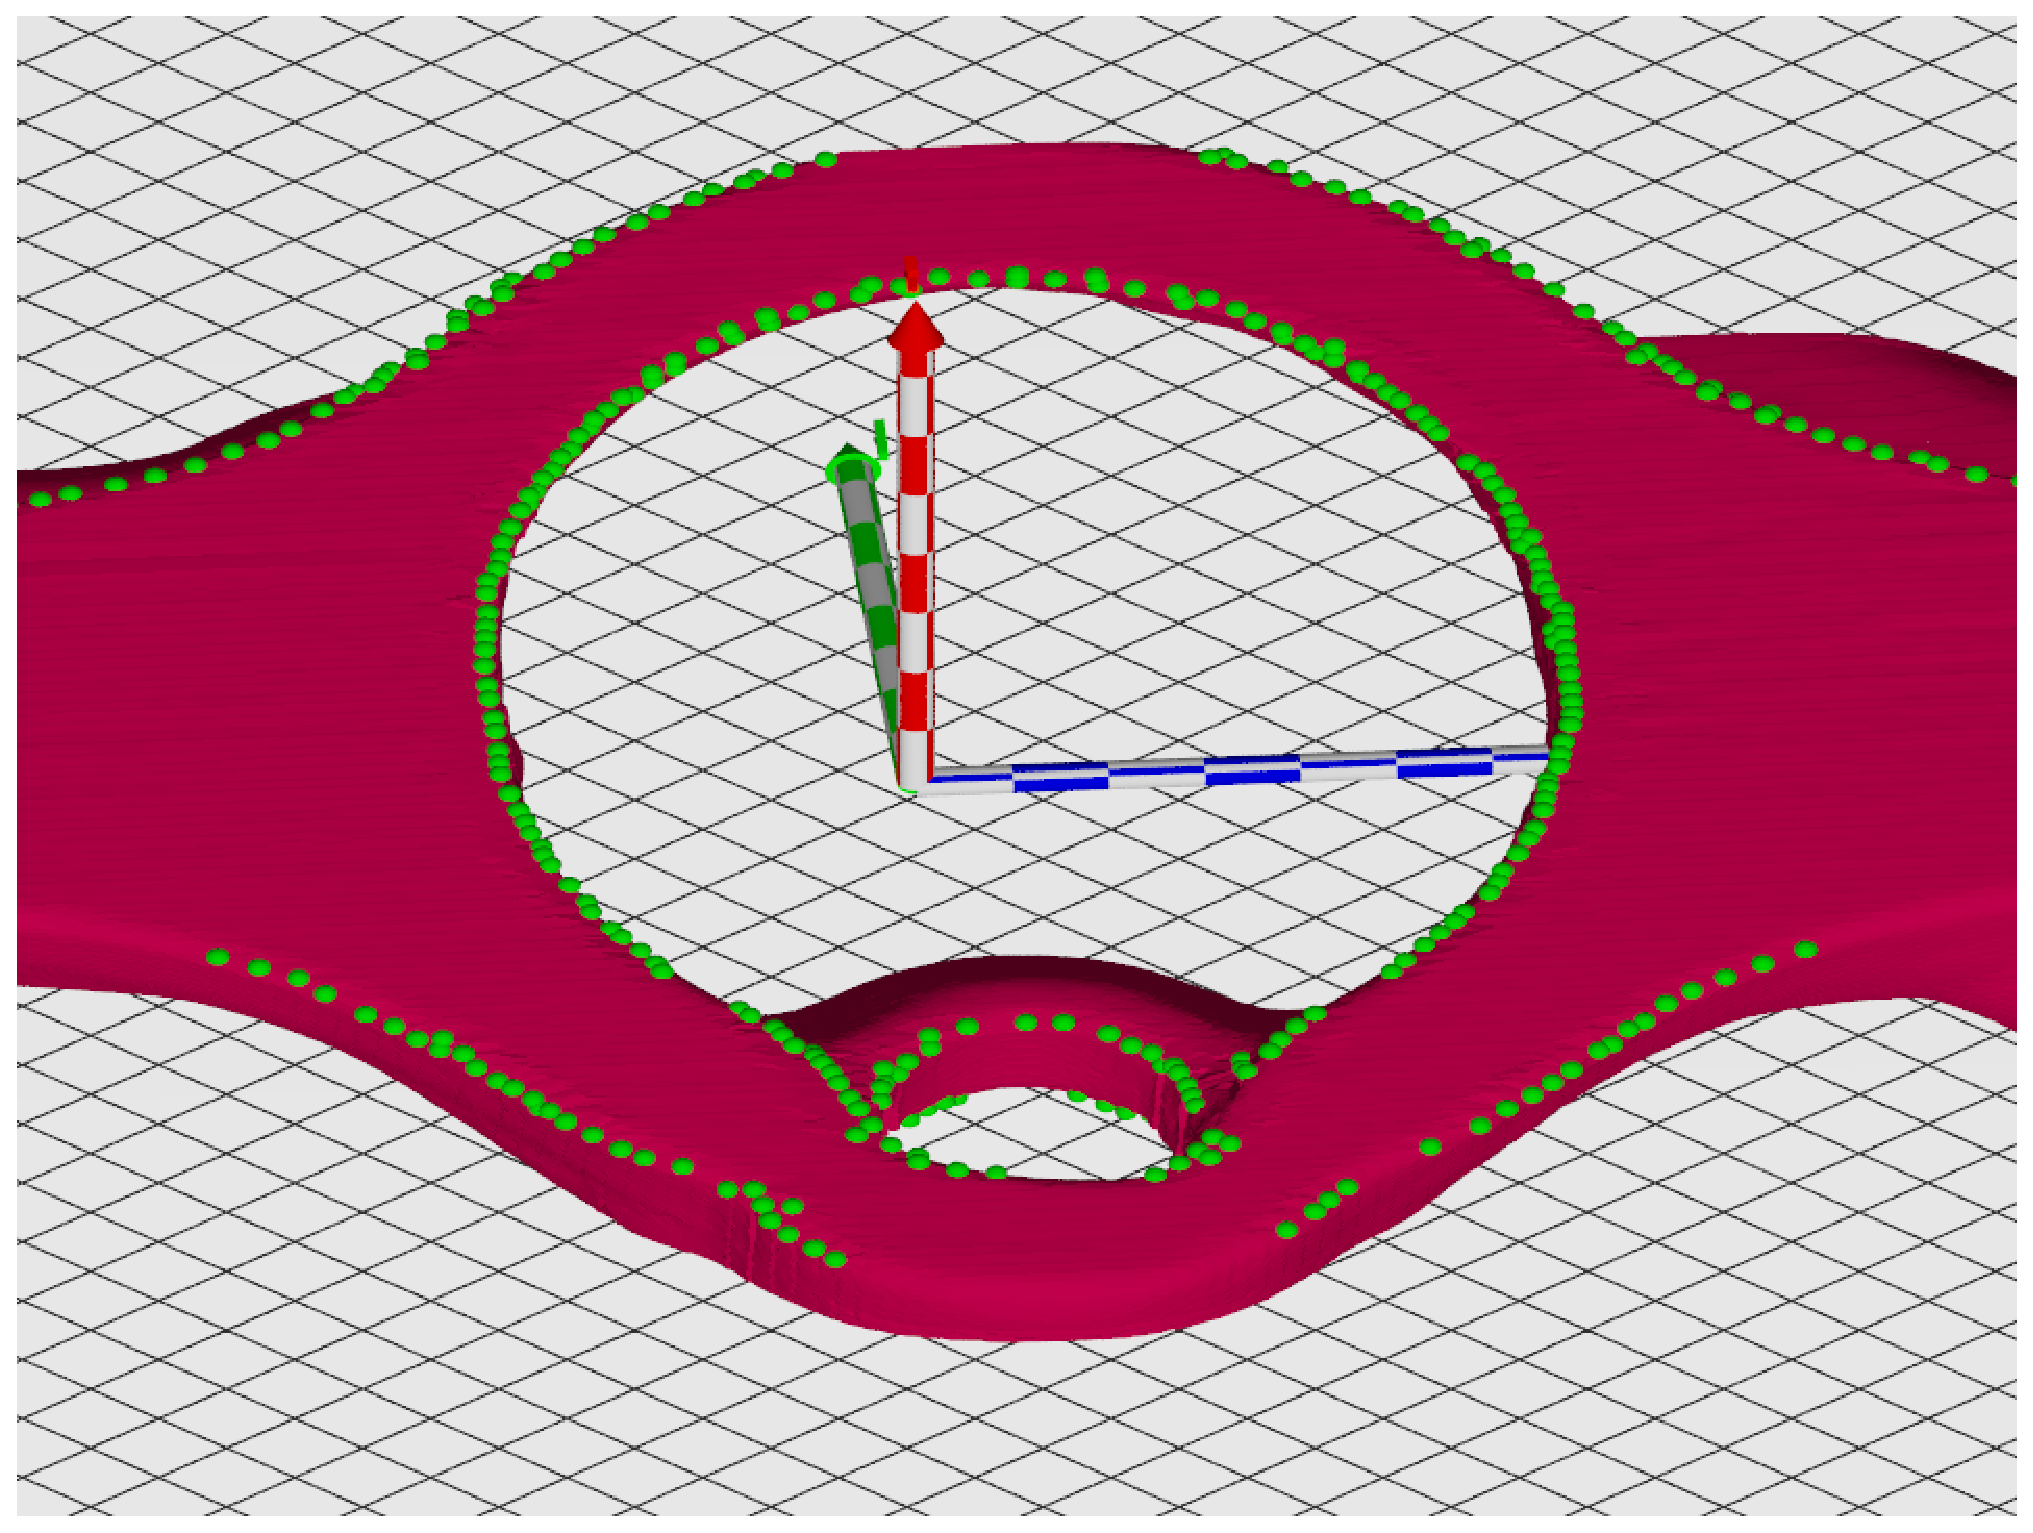
\includegraphics[width=0.32\linewidth]{images/intake.1.crop.eps}\label{fig:intake:a} }
    \subfloat[Slice]{ 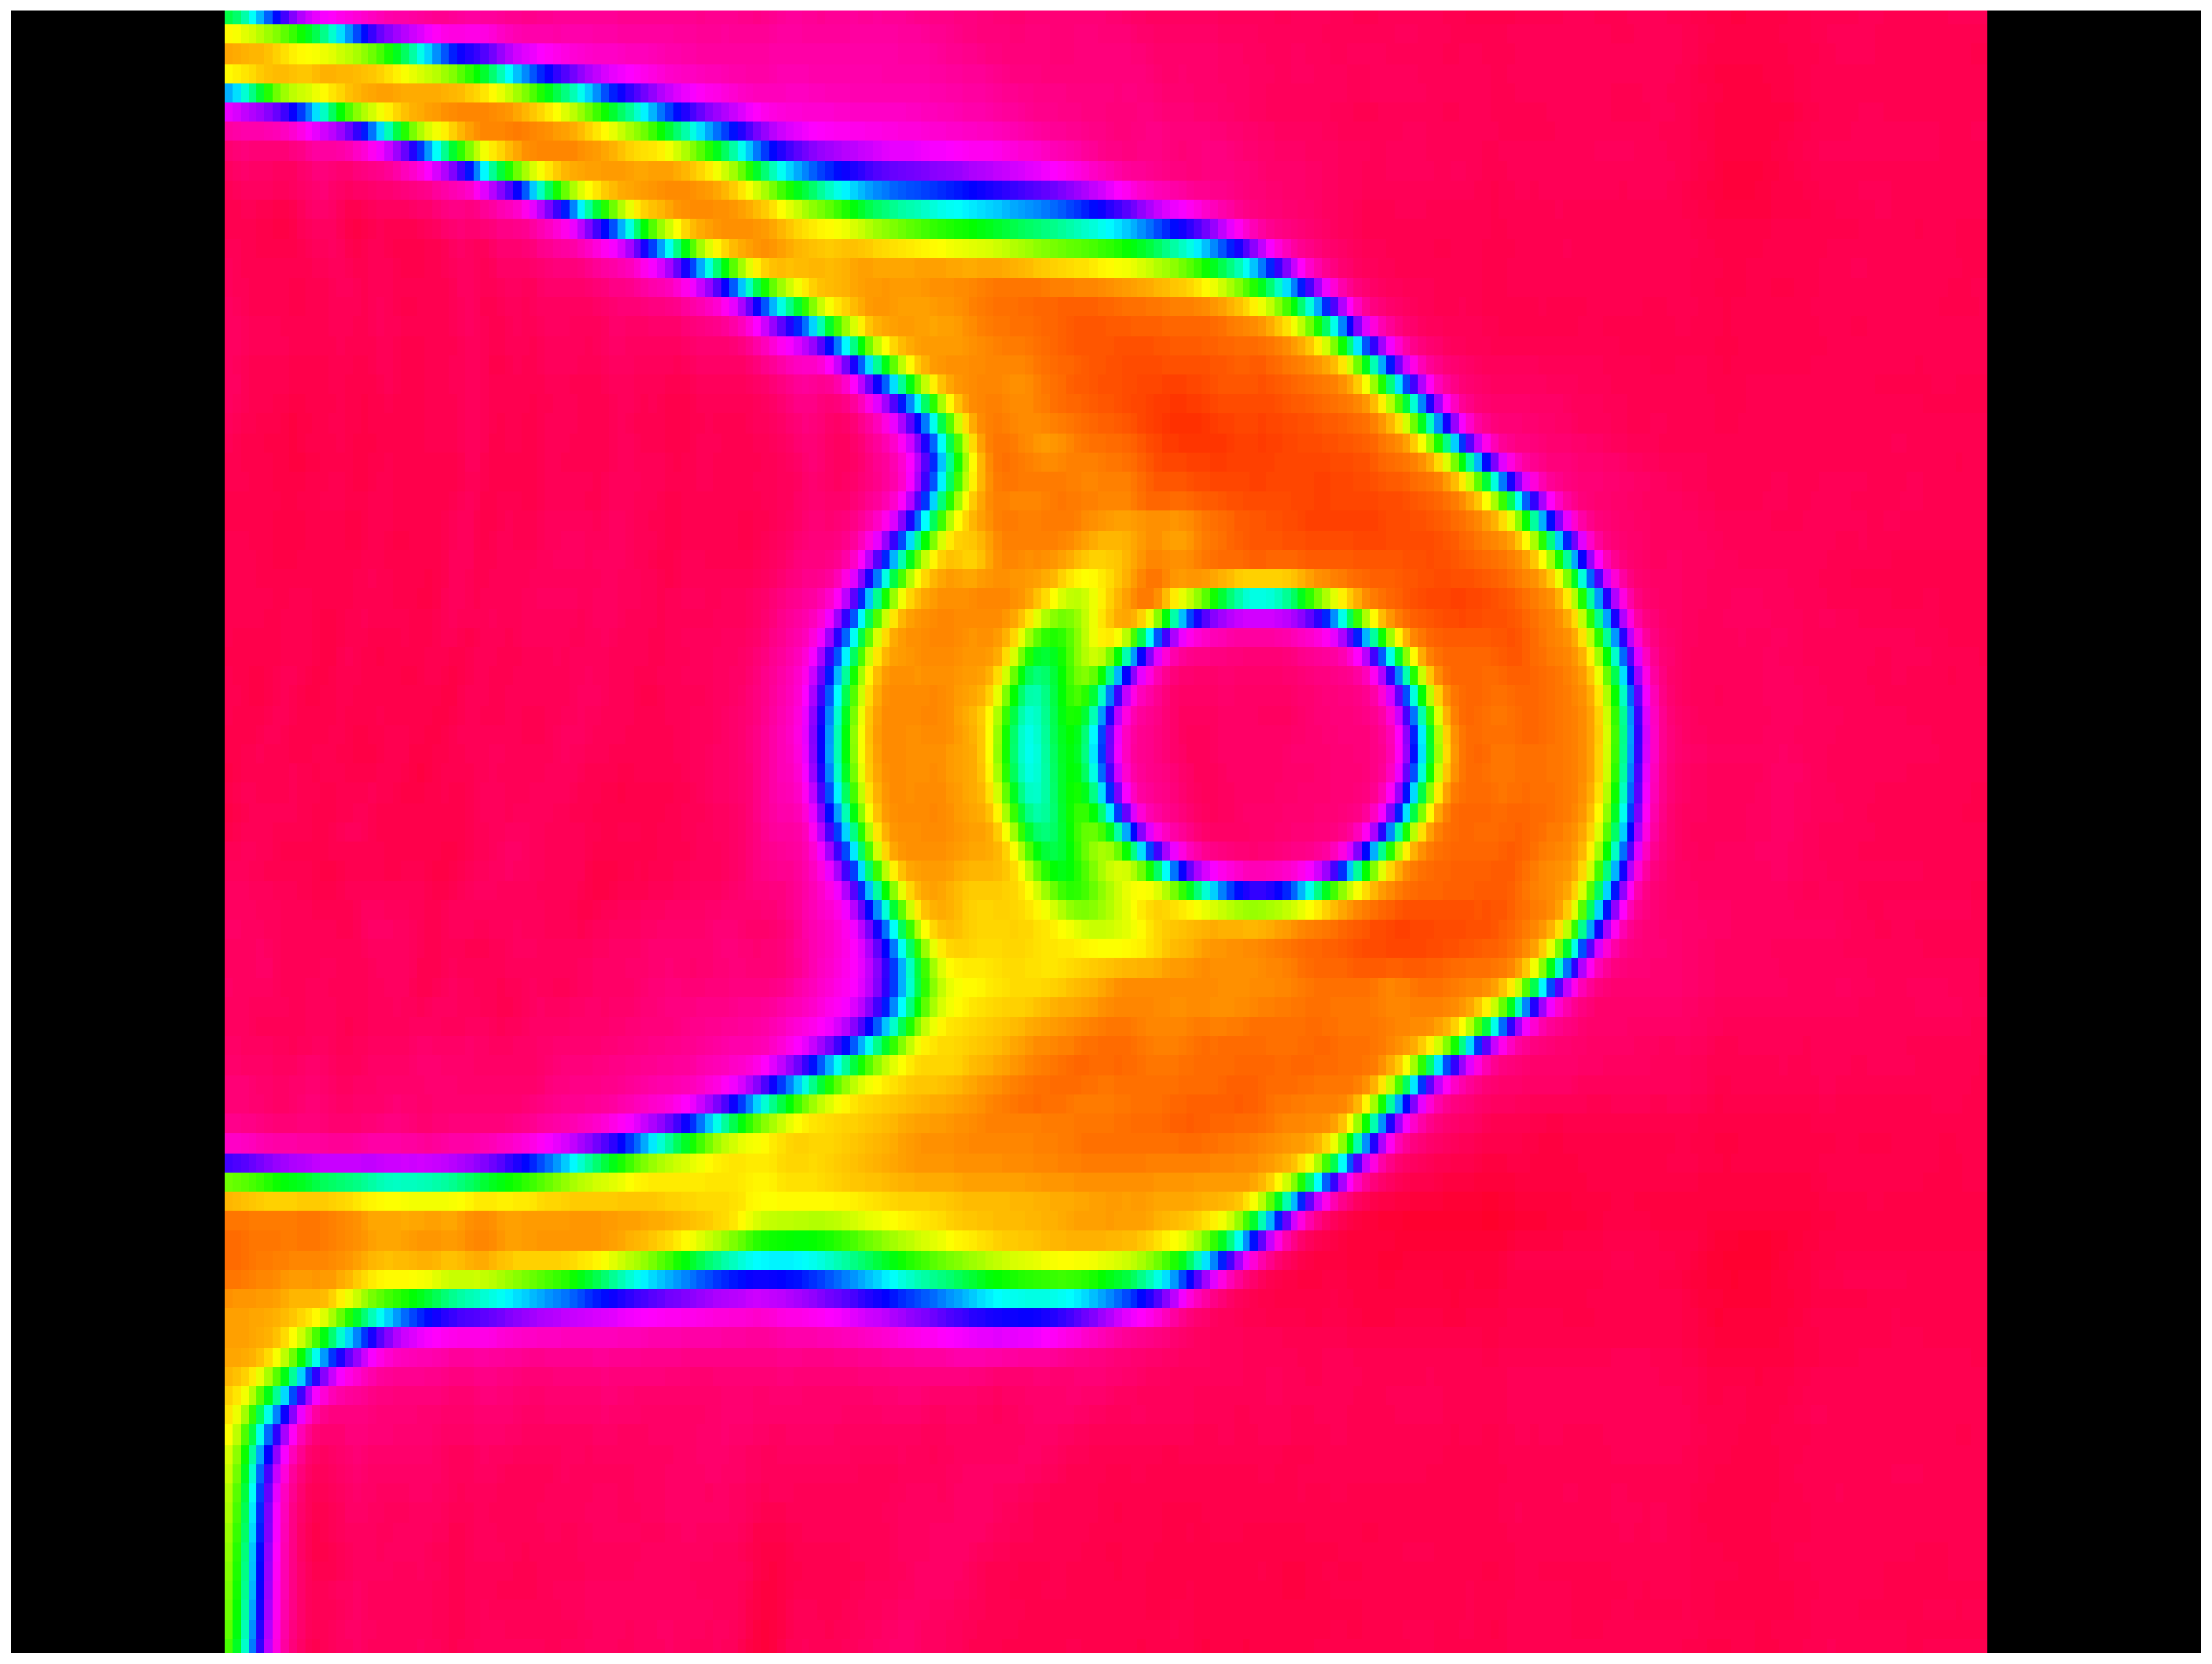
\includegraphics[width=0.32\linewidth]{images/intake.sliceYZ.eps}\label{fig:intake:b} }
    \subfloat[Context]{ 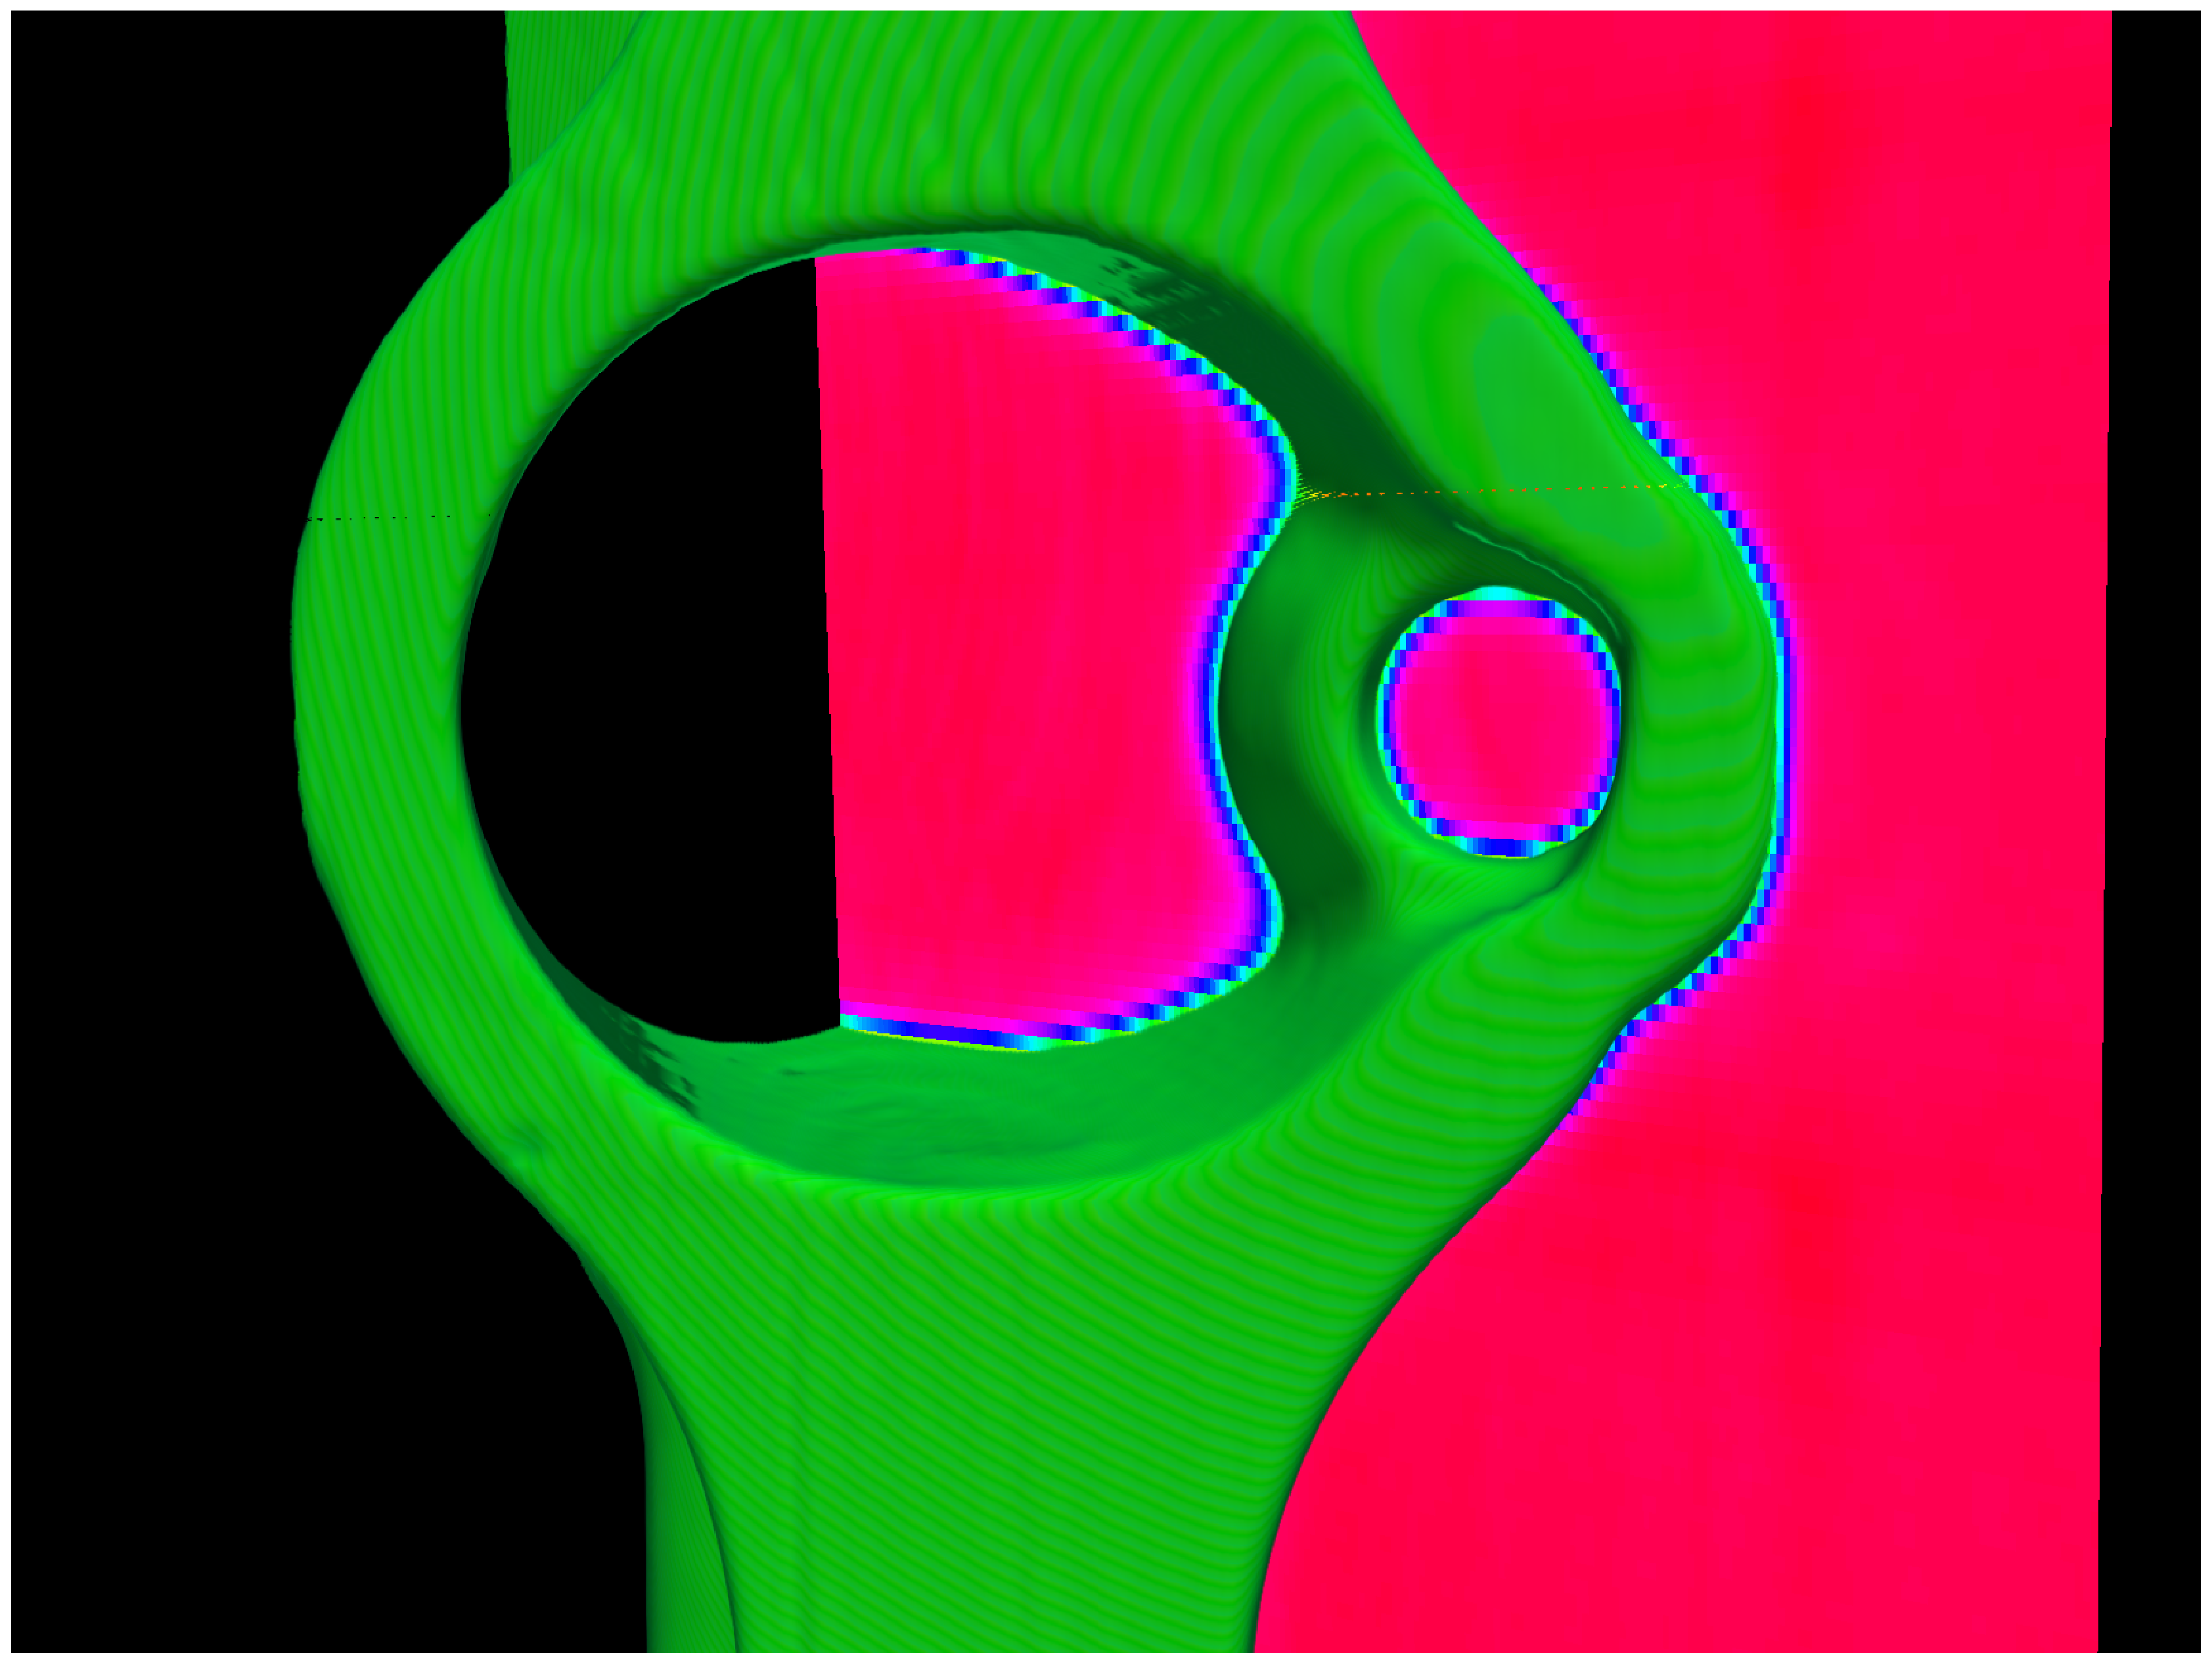
\includegraphics[width=0.32\linewidth]{images/intake.context.sliceYZ.eps}\label{fig:intake:c} }
    \caption{~\protect\subref*{fig:intake:a} shows the MergeSharp surface and point skeleton of the socket dataset.~\protect\subref{fig:intake:b} shows a single slice of the YZ axis using the hsv color scale.~\protect\subref*{fig:intake:c} the slice along with the dataset, to provide context. The dataset is not axis-aligned.}
    \label{fig:intake}
\end{figure}
 \begin{figure}[htb]
     \centering
      \subfloat[]{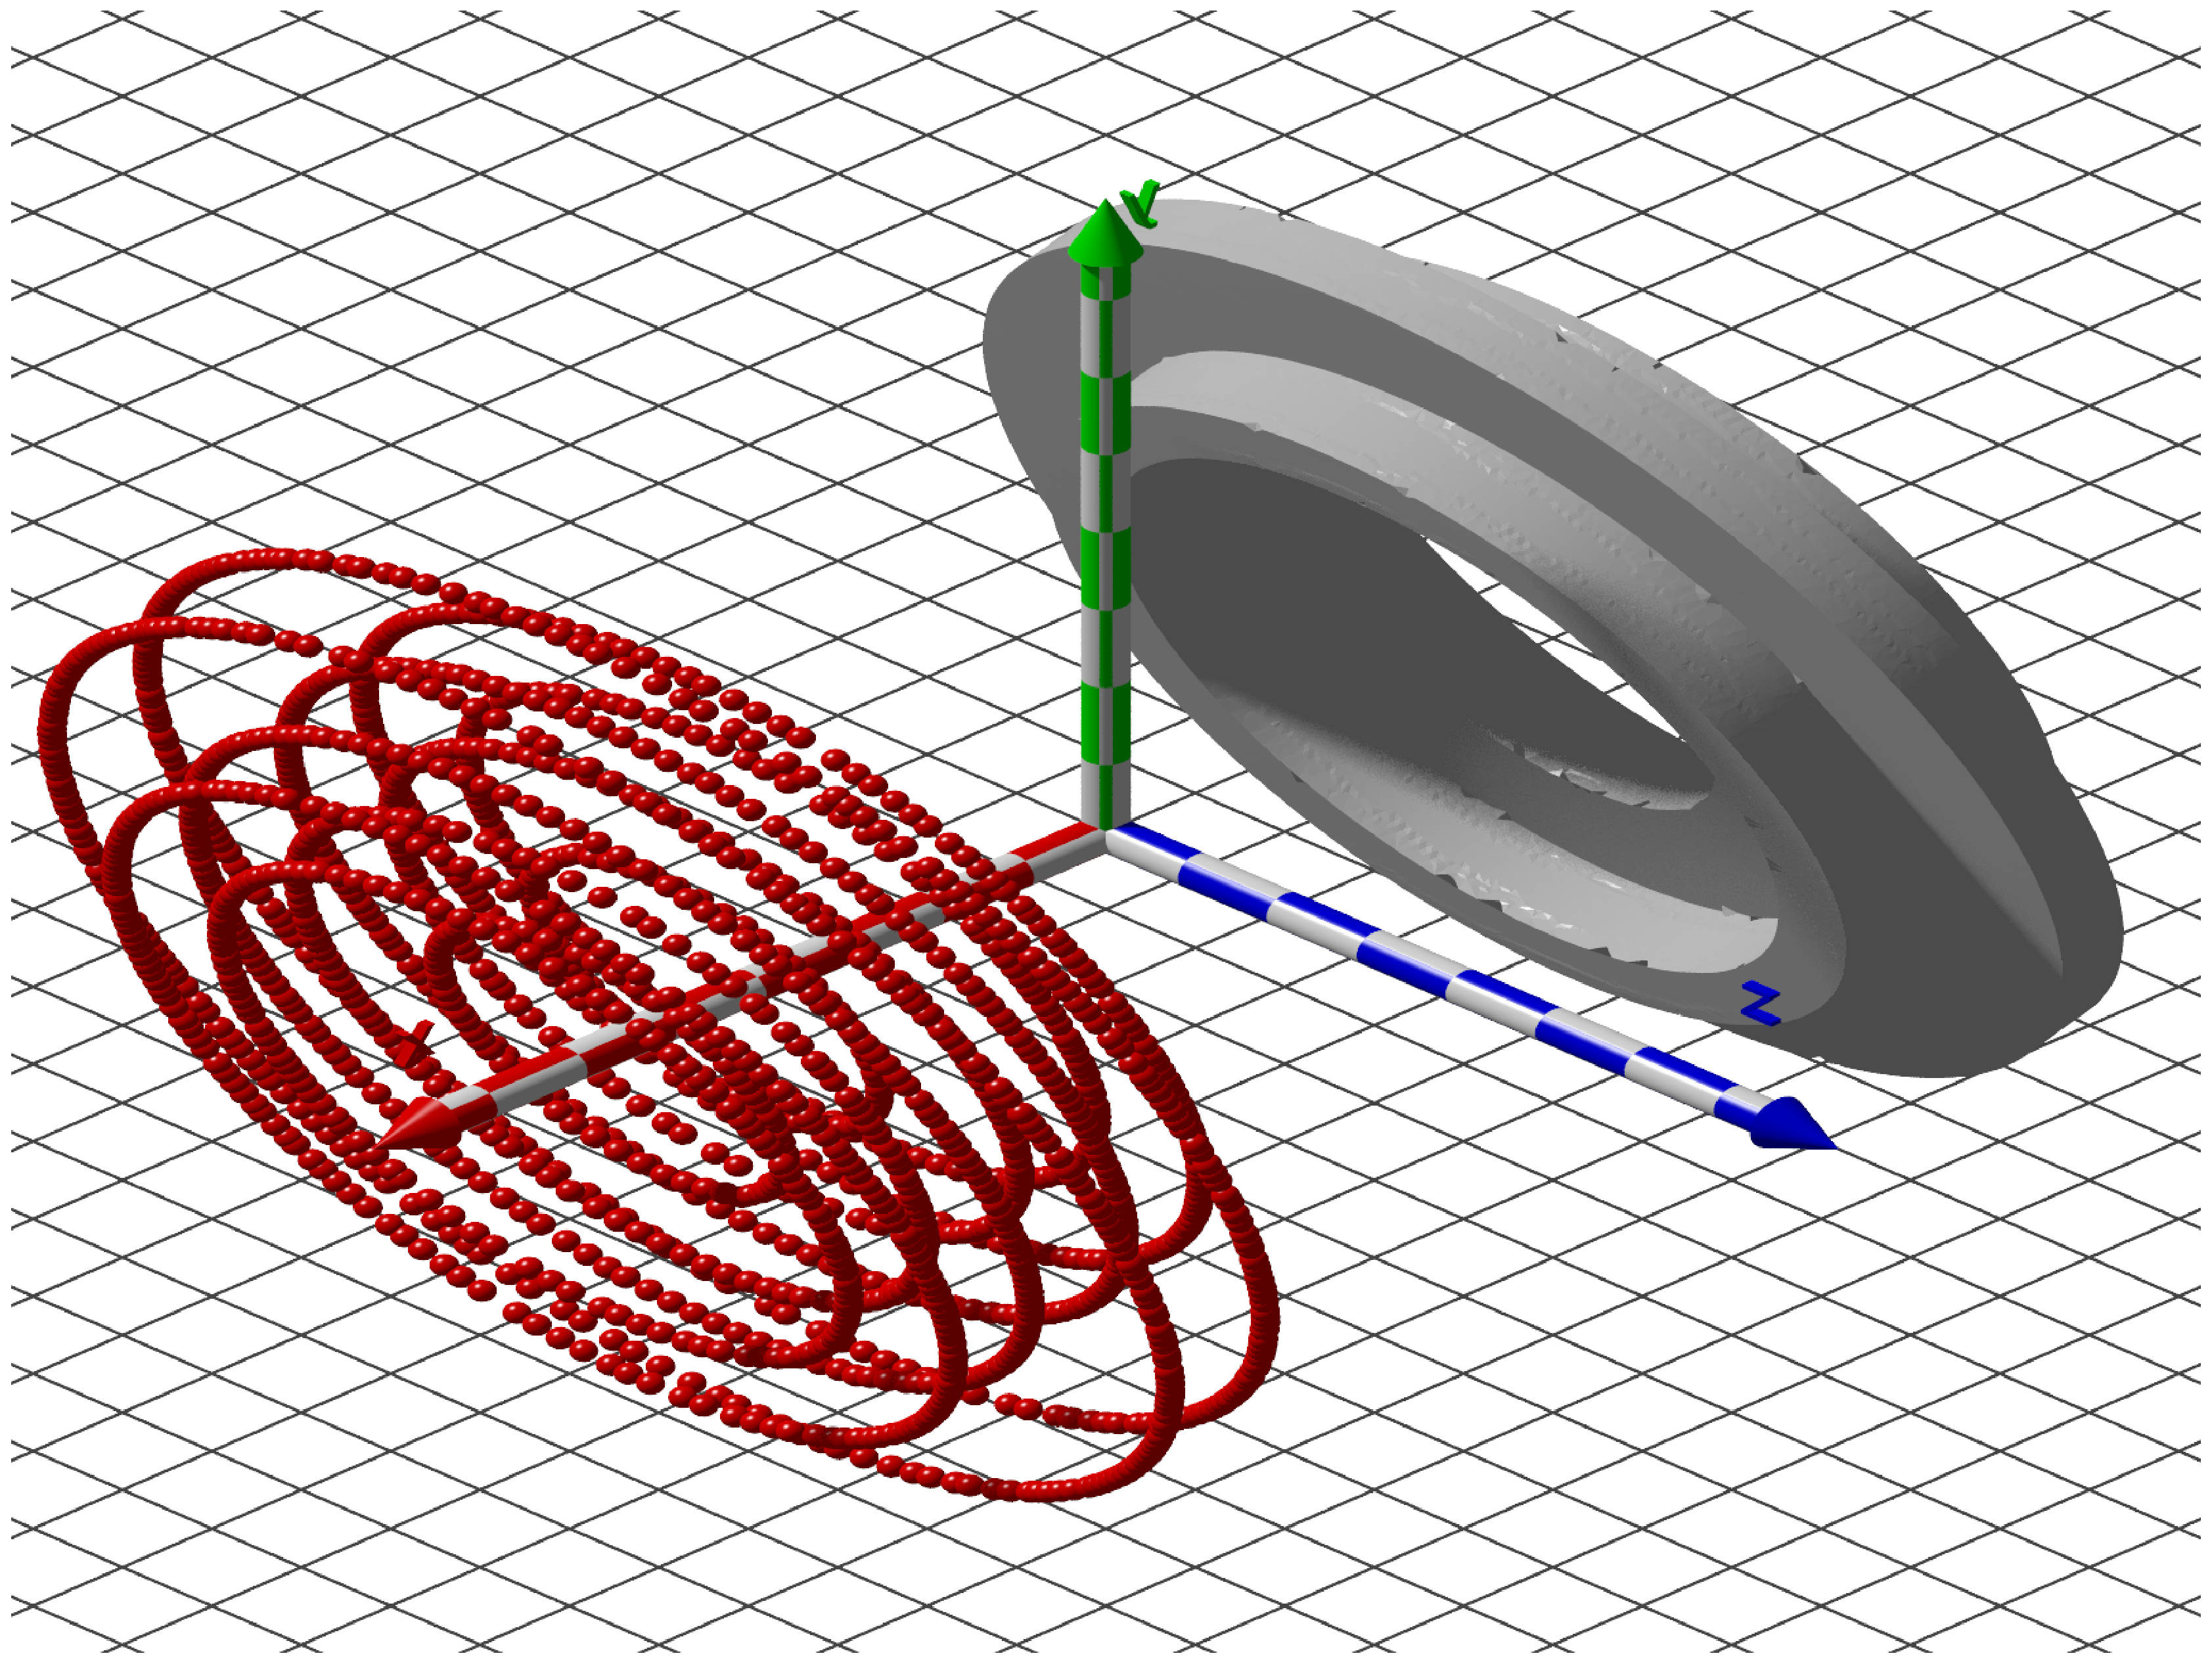
\includegraphics[width=0.33\linewidth]{images/cocone.result.eps} \label{fig:weightCocone}}
%     \subfloat[]{\includegraphics[width=0.33\linewidth]{images/fandisk.eps}
%         \label{fig:rimls}}
     \subfloat[]{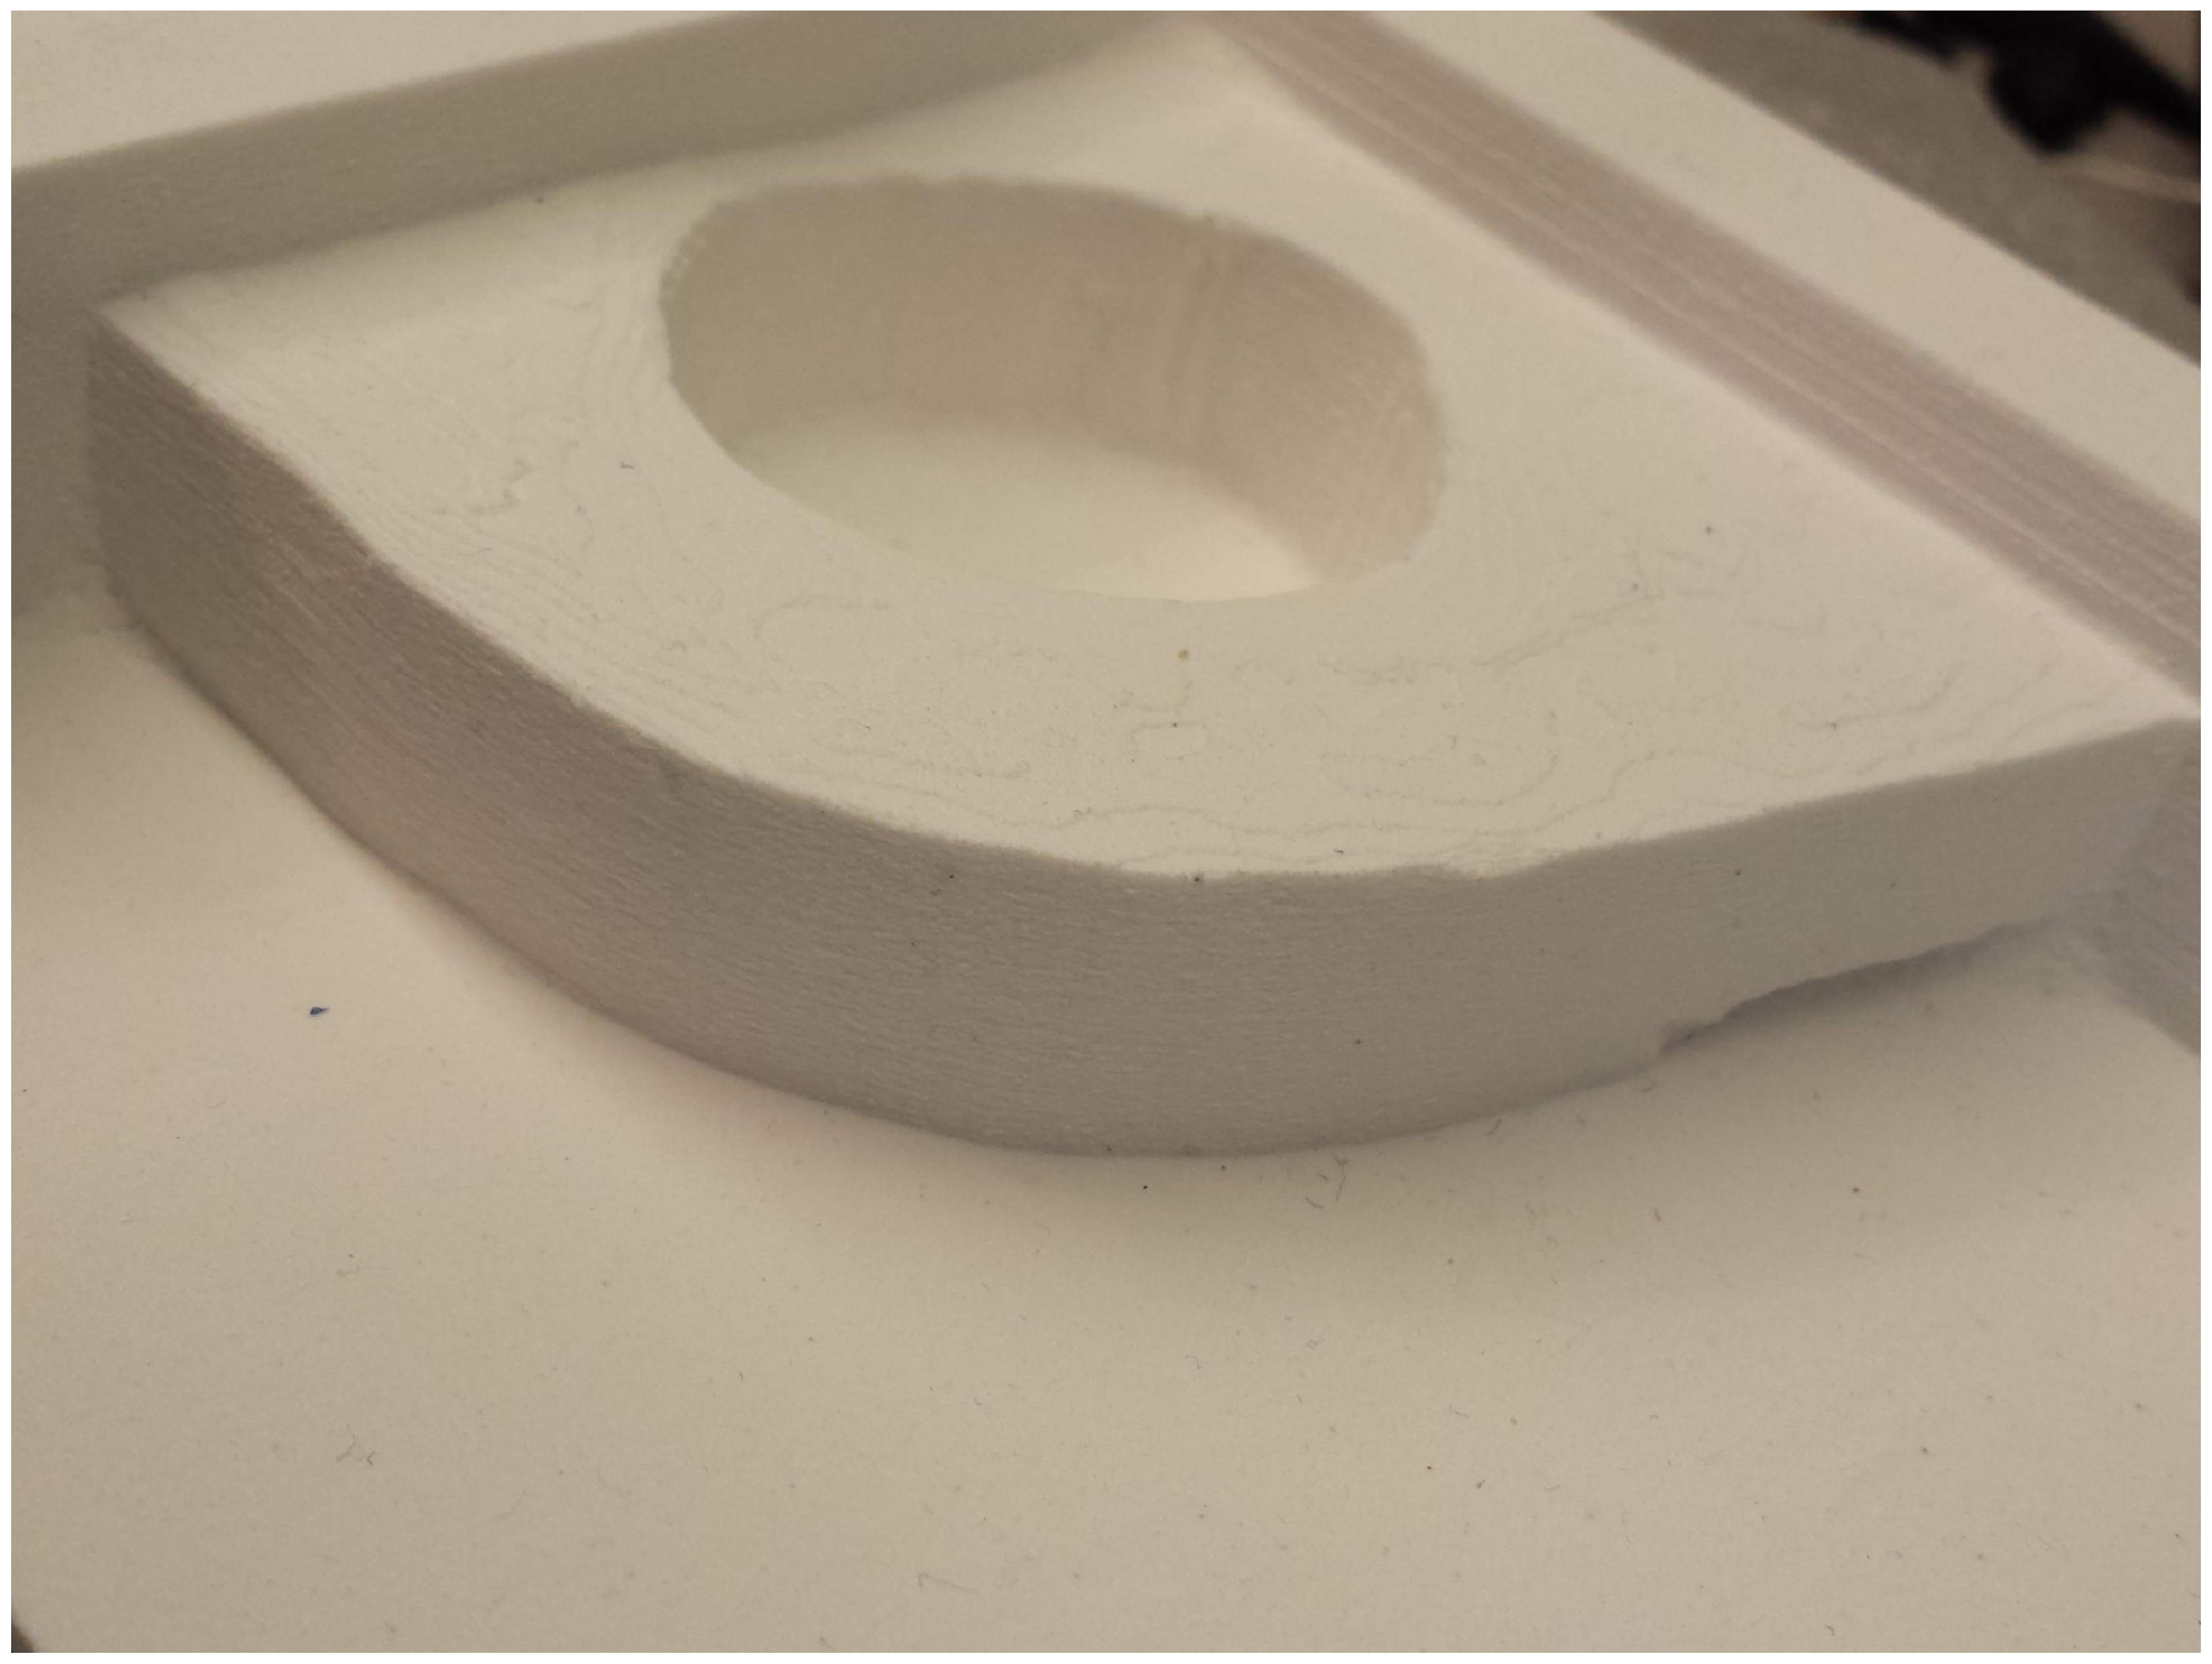
\includegraphics[width=0.33\linewidth]{images/3dscan.new.eps}
     \label{fig:3dprint}}
     \caption{ ~\protect\subref*{fig:weightCocone} shows the result of SingularCocone using the sparse selected vertices as input and the corresponding output mesh on the Flange dataset.
%         Figure~\ref{fig:rimls} shows the result of running RIMLS~\cite{Oeztireli2009}, on a point dataset containing an edge and a corner, the edges are "pinched" not actually sharp. 
          Figure~\protect\subref*{fig:3dprint} shows a 3D print of Figure~\protect\subref*{fig:setA.crop1.2}.
}
     \label{fig:fandisk}
    \end{figure}
    
\section{Conclusion and Future Work}

We showed that sharp features can be extracted directly 
from industrial CT scalar data, without extra information.
This is a major improvement over previous algorithms which require
exact surface normals or gradients.
We stress on this being a complete framework, starting directly from the CT scan, to constructing isosurface meshes with good representation of sharp edges and corners. 
Figure~\subref*{fig:3dprint} shows a 3D printing of a part of the \emph{cylinder engine} dataset.From the  mesh extracted in Figure~\subref*{fig:setA.crop1.2}.
